\documentclass[1pt, aspectratio=169,t]{beamer}

\usepackage[T1]{fontenc}
\usepackage[utf8]{inputenc}
\usepackage[slovene]{babel}
\usepackage{lmodern}
\usepackage{amsfonts,amssymb,amsmath}
\usepackage{pgfpages}
% \usepackage{tikz}
\usepackage{wrapfig}
\usepackage{graphicx}
\usepackage{pgfkeys}
\usepackage{pgfplots}
\usepackage{xcolor}
\usepackage{tkz-euclide}
\usepackage{xfp}
% \usepackage{pgf}
\usepackage{colortbl}
\usepackage{hhline}
\usepackage{longtable}
\usepackage{multicol}
\usepackage{wasysym}
\usepackage[gen]{eurosym}
\usepackage{newunicodechar}
\newunicodechar{€}{\euro}


\pgfplotsset{compat=1.18} 

\usetikzlibrary{angles,arrows,arrows.meta,calc,decorations,decorations.markings,decorations.pathreplacing,decorations.shapes,decorations.text,
	decorations.pathmorphing,intersections,math,plotmarks,positioning,quotes,shapes.misc,through}



% \setbeameroption{show notes on second screen}
% \setbeameroption{show only notes}

% \usetheme[sectionpage=simple, titlestyle=plain, sectionstyle=style2, slidestyle=style1, numbering=counter, block=fill, headingcolor=theme]{trigon}

\usetheme{CambridgeUS}
\usecolortheme{beaver}



\setbeamerfont{subtitle}{size=\small}


\title{MATEMATIKA}
\subtitle{2. letnik -- splošna gimnazija}
\date{\today}
\author{Jan Kastelic}
\institute[GAA]{Gimnazija Antona Aškerca, \\ Šolski center Ljubljana}

\newtheorem{izrek}{Izrek}
\newcommand{\Vir}[1]{\color{gray}{\tiny{Vir: #1}}}


\begin{document}

\begin{frame}
	\titlepage
\end{frame}
	
% \titleframe

\begin{frame}
	\frametitle{Vsebina}
	\tableofcontents[hideallsubsections]
\end{frame}
	
% \section{Geometrija v ravnini}

\begin{frame}
    \sectionpage
\end{frame}

\begin{frame}
    \tableofcontents[currentsection, hideothersubsections]
\end{frame}

%%%%%%%%%%%%%%%%%%%%%%%%%%%%%%%%%%%%%%
    \subsection{Osnovni geometrijski pojmi}

        \begin{frame}
            \frametitle{Osnovni geometrijski pojmi}

            \begin{block}{}
                Evklid je v prvi knjigi \textit{Elementov} postavil $23$ 'opredelitev' temeljnih geometrijskih pojmov.
                Med njimi so:
                \begin{itemize}
                    \item \textbf{Točka} je tisto, kar nima delov -- nima razsežnosti.
                    \item \textbf{Črta} je dolžina brez širine -- ena razsežnost.
                    \item \textbf{Ploskev} je tisto, kar ima samo dolžino in širino -- dve razsežnosti.
                \end{itemize}
            \end{block}

            \begin{block}{}
                Tem trditvam sledijo \textbf{aksiomi} (temeljne resnice) -- privzamemo jih kot veljavne hipoteze,
                 \textbf{izreki}~-- dokazujemo jih z aksiomi in prej dokazanimi izreki, 
                 in \textbf{definicije} -- opisi novih pojmov in lastnosti.
            \end{block}
        \end{frame}

        \begin{frame}
            \frametitle{Incidenčni aksiomi}

            \vskip-1em
            \begin{alertblock}{Definicija}
                \textit{Incidenca} je relacija, ki povezuje točko in premico -- premica in točka sta v relaciji,
                 če točka leži na premici; $A~R~p$, če $A\in p$.
            \end{alertblock}

            \begin{alertblock}{Aksiom 1}
                Za dve različni točki $A$ in $B$ obstaja natanko določena premica $p$, tako da točki $A$ in $B$ ležita na njej.
            \end{alertblock}

            \begin{alertblock}{Aksiom 2}
                Za vsako premico $p$ obstajata vsaj dve različni točki $P$ in $Q$, ki ležita na njej.
            \end{alertblock}

            \begin{alertblock}{Aksiom 3}
                Obstajajo tri različne točke, ki ne ležijo hkrati na isti premici.
            \end{alertblock}
        \end{frame}


        \begin{frame}
            \begin{alertblock}{Definicija}
                Točke $A_1, A_2, A_3, \dots$, ki ležijo na isti premici, so \textbf{kolinearne}, 
                če ne ležijo na isti premici, pa so \textbf{nekolinearne}.
            \end{alertblock}

            \begin{block}{Izrek}
                Dve različni premici imata lahko največ eno skupno točko.
            \end{block}

            \begin{alertblock}{Definicija}
                Premici, ki imata natanko eno skupno točko, se \textbf{sekata}, imenujemo ju \textbf{sečnici},
                njuno skupno točko pa \textbf{presečišče} premic.
            \end{alertblock}

            \begin{alertblock}{Definicija}
                Premici, ki ležita na isti ravnini in nimata nobene skupne točke ali imata vse točke skupne -- sovpadata, sta \textbf{vzporedni}, imenujemo ju \textbf{vzporednici}.
            \end{alertblock}
        \end{frame}


        \begin{frame}
            \begin{alertblock}{Aksiom}
                Če so tri različne točke kolinearne, ena vedno leži med drugima dvema.

                \begin{figure}[H]
                    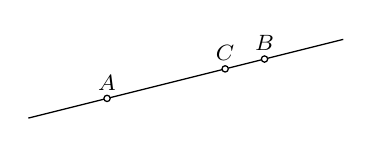
\begin{tikzpicture}
                        % \clip (0,0) rectangle (14.000000,10.000000);
                        {\footnotesize

                        % Drawing line A B
                        \draw [line width=0.016cm] (1.000000,1.250000) -- (1.961194,1.490299);%
                        \draw [line width=0.016cm] (2.038806,1.509701) -- (3.461194,1.865299);%
                        \draw [line width=0.016cm] (3.538806,1.884701) -- (3.961194,1.990299);%
                        \draw [line width=0.016cm] (4.038806,2.009701) -- (5.000000,2.250000);%

                        % Marking point A by circle
                        \draw [line width=0.016cm] (2.000000,1.500000) circle (0.040000);%
                        \draw (2.000000,1.500000) node [anchor=south] { $A$ };%

                        % Marking point C by circle
                        \draw [line width=0.016cm] (3.500000,1.875000) circle (0.040000);%
                        \draw (3.500000,1.875000) node [anchor=south] { $C$ };%

                        % Marking point B by circle
                        \draw [line width=0.016cm] (4.000000,2.000000) circle (0.040000);%
                        \draw (4.000000,2.000000) node [anchor=south] { $B$ };%
                        }
                    \end{tikzpicture}
                \end{figure}
            \end{alertblock}

            \begin{alertblock}{Aksiom}
                Če sta $A$ in $B$ različni točki premice $p$, potem na premici $p$ ležita vsaj še točki $C$ in $D$,
                in sicer $C$ leži med $A$ in $B$, $D$ pa tako, da je $C$ med $A$ in $D$.

                \begin{figure}[H]
                    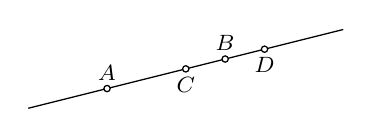
\begin{tikzpicture}
                        % \clip (0,0) rectangle (14.000000,10.000000);
                        {\footnotesize

                        % Drawing line A B
                        \draw [line width=0.016cm] (1.000000,1.250000) -- (1.961194,1.490299);%
                        \draw [line width=0.016cm] (2.038806,1.509701) -- (2.961194,1.740299);%
                        \draw [line width=0.016cm] (3.038806,1.759701) -- (3.461194,1.865299);%
                        \draw [line width=0.016cm] (3.538806,1.884701) -- (3.961194,1.990299);%
                        \draw [line width=0.016cm] (4.038806,2.009701) -- (5.000000,2.250000);%

                        % Marking point A by circle
                        \draw [line width=0.016cm] (2.000000,1.500000) circle (0.040000);%
                        \draw (2.000000,1.500000) node [anchor=south] { $A$ };%

                        % Marking point C by circle
                        \draw [line width=0.016cm] (3.000000,1.750000) circle (0.040000);%
                        \draw (3.000000,1.750000) node [anchor=north] { $C$ };%

                        % Marking point B by circle
                        \draw [line width=0.016cm] (3.500000,1.875000) circle (0.040000);%
                        \draw (3.500000,1.875000) node [anchor=south] { $B$ };%

                        % Marking point D by circle
                        \draw [line width=0.016cm] (4.000000,2.000000) circle (0.040000);%
                        \draw (4.000000,2.000000) node [anchor=north] { $D$ };%
                        }
                    \end{tikzpicture}
                \end{figure}
            \end{alertblock}

            \begin{block}{Izrek}
                Med dvema različnima točkama premice je neskončno mnogo točk.
            \end{block}

        \end{frame}
        

        \begin{frame}
            \begin{alertblock}{Definicija}
                Množica točk premice, ki ležijo med različnima točkama $A$ in $B$, vključno z $A$ in $B$,
                je \textbf{daljica~$AB$}. Točki $A$ in $B$ sta njeni \textbf{krajišči}.

                \begin{figure}[H]
                    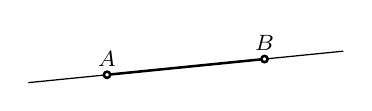
\begin{tikzpicture}
                        % \clip (0,0) rectangle (14.000000,10.000000);
                        {\footnotesize

                        % Drawing line A B
                        \draw [line width=0.016cm] (1.000000,1.400000) -- (1.960199,1.496020);%
                        \draw [line width=0.016cm] (2.039801,1.503980) -- (3.960199,1.696020);%
                        \draw [line width=0.016cm] (4.039801,1.703980) -- (5.000000,1.800000);%

                        % Drawing segment A B
                        \draw [line width=0.032cm] (2.039801,1.503980) -- (3.960199,1.696020);%

                        % Marking point A by circle
                        \draw [line width=0.032cm] (2.000000,1.500000) circle (0.040000);%
                        \draw (2.000000,1.500000) node [anchor=south] { $A$ };%

                        % Marking point B by circle
                        \draw [line width=0.032cm] (4.000000,1.700000) circle (0.040000);%
                        \draw (4.000000,1.700000) node [anchor=south] { $B$ };%
                        }
                    \end{tikzpicture}
                \end{figure}
            \end{alertblock}

            \begin{alertblock}{Definicija}
                Poljubna točka premice razdeli premico na dva \textbf{poltraka}. To točko imenujemo \textbf{izhodišče}, ponavadi jo označimo z $O$.

                \begin{figure}[H]
                    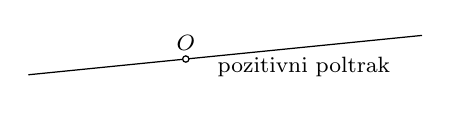
\begin{tikzpicture}
                        % \clip (0,0) rectangle (14.000000,10.000000);
                        {\footnotesize

                        % Drawing line O B
                        \draw [line width=0.016cm] (1.000000,1.300000) -- (2.960199,1.496020);%
                        \draw [line width=0.016cm] (3.039801,1.503980) -- (6.000000,1.800000);%

                        % Marking point O by circle
                        \draw [line width=0.016cm] (3.000000,1.500000) circle (0.040000);%
                        \draw (3.000000,1.500000) node [anchor=south] { $O$ };%

                        % Marking point poz
                        \draw (4.500000,1.400000) node  {pozitivni poltrak };%
                        }
                    \end{tikzpicture}
                \end{figure}
            \end{alertblock}

            \begin{alertblock}{Definicija}
                Premica, na kateri leži daljica oziroma poltrak, je \textbf{nosilka} daljice oziroma poltraka.
            \end{alertblock}
        \end{frame}


        \begin{frame}
            \begin{alertblock}{Definicija}
                \textbf{Enostavni lik} je množica točk v ravnini, ki jo omejuje sklenjena krivulja, ki sama sebe ne seka.
            \end{alertblock}

            \begin{alertblock}{Definicija}
                \begin{columns}
                    \column{0.75\textwidth}

                Množica točk v ravnini je \textbf{konveksna}, če za poljubni točki $A$ in $B$ iz te množice velja, da je daljica $AB$ njena podmnožica.
                $$ \mathcal{M}\text{~konveksna} \Leftrightarrow \forall A, B\in\mathcal{M}\Rightarrow AB\subseteq\mathcal{M} $$
                Množica točk, ki ni konveksna, je \textbf{nekonveksna} oziroma \textbf{konkavna}.
                $$ \mathcal{M}\text{~nekonveksna} \Leftrightarrow \exists A, B\in\mathcal{M}\Rightarrow AB\not\subset\mathcal{M} $$
            
                \column{0.22\textwidth}
                \begin{figure}[H]
                    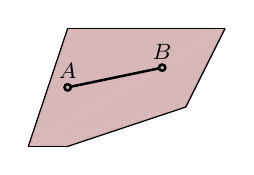
\begin{tikzpicture}
                        % \clip (0,0) rectangle (14.000000,10.000000);
                        {\footnotesize

                        % Changing color 215 183 183
                        \definecolor{r215g183b183}{rgb}{0.843137,0.717647,0.717647}%
                        \color{r215g183b183}% 

                        % Filling triangle C D E
                        \fill (1.500000,1.500000) -- (2.000000,1.500000) -- (3.500000,2.000000);%

                        % Filling triangle C E F
                        \fill (1.500000,1.500000) -- (3.500000,2.000000) -- (4.000000,3.000000);%

                        % Filling triangle C F G
                        \fill (1.500000,1.500000) -- (4.000000,3.000000) -- (2.000000,3.000000);%

                        % Changing color 0 0 0
                        \definecolor{r0g0b0}{rgb}{0.000000,0.000000,0.000000}%
                        \color{r0g0b0}% 

                        % Drawing segment C D
                        \draw [line width=0.016cm] (1.500000,1.500000) -- (2.000000,1.500000);%

                        % Drawing segment D E
                        \draw [line width=0.016cm] (2.000000,1.500000) -- (3.500000,2.000000);%

                        % Drawing segment E F
                        \draw [line width=0.016cm] (3.500000,2.000000) -- (4.000000,3.000000);%

                        % Drawing segment F G
                        \draw [line width=0.016cm] (4.000000,3.000000) -- (2.000000,3.000000);%

                        % Drawing segment G C
                        \draw [line width=0.016cm] (2.000000,3.000000) -- (1.500000,1.500000);%

                        % Marking point A by circle
                        \draw [line width=0.032cm] (2.000000,2.250000) circle (0.040000);%
                        \draw (2.000000,2.250000) node [anchor=south] { $A$ };%

                        % Marking point B by circle
                        \draw [line width=0.032cm] (3.200000,2.500000) circle (0.040000);%
                        \draw (3.200000,2.500000) node [anchor=south] { $B$ };%

                        % Drawing segment A B
                        \draw [line width=0.032cm] (2.039159,2.258158) -- (3.160841,2.491842);%
                        \color{black}
                        }
                    \end{tikzpicture}
                \end{figure}

                \begin{figure}[H]
                    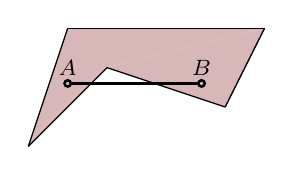
\begin{tikzpicture}
                        % \clip (0,0) rectangle (14.000000,10.000000);
                        {\footnotesize

                        % Changing color 215 183 183
                        \definecolor{r215g183b183}{rgb}{0.843137,0.717647,0.717647}%
                        \color{r215g183b183}% 

                        % Filling triangle C D G
                        \fill (1.500000,1.500000) -- (2.500000,2.500000) -- (2.000000,3.000000);%

                        % Filling triangle D E F
                        \fill (2.500000,2.500000) -- (4.000000,2.000000) -- (4.500000,3.000000);%

                        % Filling triangle D F G
                        \fill (2.500000,2.500000) -- (4.500000,3.000000) -- (2.000000,3.000000);%

                        % Changing color 0 0 0
                        \definecolor{r0g0b0}{rgb}{0.000000,0.000000,0.000000}%
                        \color{r0g0b0}% 

                        % Drawing segment C D
                        \draw [line width=0.016cm] (1.500000,1.500000) -- (2.500000,2.500000);%

                        % Drawing segment D E
                        \draw [line width=0.016cm] (2.500000,2.500000) -- (4.000000,2.000000);%

                        % Drawing segment E F
                        \draw [line width=0.016cm] (4.000000,2.000000) -- (4.500000,3.000000);%

                        % Drawing segment F G
                        \draw [line width=0.016cm] (4.500000,3.000000) -- (2.000000,3.000000);%

                        % Drawing segment G C
                        \draw [line width=0.016cm] (2.000000,3.000000) -- (1.500000,1.500000);%

                        % Marking point A by circle
                        \draw [line width=0.032cm] (2.000000,2.300000) circle (0.040000);%
                        \draw (2.000000,2.300000) node [anchor=south] { $A$ };%

                        % Marking point B by circle
                        \draw [line width=0.032cm] (3.700000,2.300000) circle (0.040000);%
                        \draw (3.700000,2.300000) node [anchor=south] { $B$ };%

                        % Drawing segment A B
                        \draw [line width=0.032cm] (2.040000,2.300000) -- (3.660000,2.300000);%
                        \color{black}
                        }
                    \end{tikzpicture}
                \end{figure}
                \end{columns}

            \end{alertblock}
        \end{frame}


        \begin{frame}
            \begin{alertblock}{Definicija}
                \begin{columns}
                    \column{0.6\textwidth}
                Dva poltraka s skupnim izhodiščem določata dva \textbf{kota}.
                Izhodišče poltrakov imenujemo \textbf{vrh} kota, poltraka pa imenujemo \textbf{kraka} kota.
                
                \column{0.38\textwidth}
                \vskip-2em
                \begin{figure}[H]
                    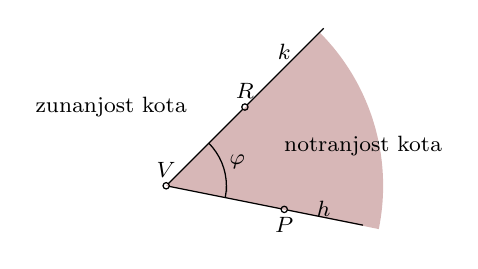
\begin{tikzpicture}
                        % \clip (0,0) rectangle (14.000000,10.000000);
                        {\footnotesize

                        % Changing color 215 183 183
                        \definecolor{r215g183b183}{rgb}{0.843137,0.717647,0.717647}%
                        \color{r215g183b183}% 

                        % Filling circle arc V B 56.31
                        \fill (2.500000,2.500000) -- (5.200000,1.949999) -- (5.204824,1.974235) arc (349:360:2.755449 and 2.755449) --(5.255449,2.500000) arc (0:44:2.755449 and 2.755449) -- (4.455318,4.441451) -- cycle;%

                        % Changing color 0 0 0
                        \definecolor{r0g0b0}{rgb}{0.000000,0.000000,0.000000}%
                        \color{r0g0b0}% 

                        % Drawing line V P
                        % \draw [line width=0.016cm] (1.000000,2.800000) -- (2.460777,2.507845);%
                        \draw [line width=0.016cm] (2.539223,2.492155) -- (3.960777,2.207845);%
                        \draw [line width=0.016cm] (4.039223,2.192155) -- (5.000000,2.000000);%

                        % Drawing line V R
                        % \draw [line width=0.016cm] (1.000000,1.000000) -- (2.471716,2.471716);%
                        \draw [line width=0.016cm] (2.528284,2.528284) -- (3.471716,3.471716);%
                        \draw [line width=0.016cm] (3.528284,3.528284) -- (4.500000,4.500000);%

                        % Marking point V by circle
                        \draw [line width=0.016cm] (2.500000,2.500000) circle (0.040000);%
                        \draw (2.500000,2.500000) node [anchor=south] { $V$ };%

                        % Marking point P by circle
                        \draw [line width=0.016cm] (4.000000,2.200000) circle (0.040000);%
                        \draw (4.000000,2.200000) node [anchor=north] { $P$ };%

                        % Marking point R by circle
                        \draw [line width=0.016cm] (3.500000,3.500000) circle (0.040000);%
                        \draw (3.500000,3.500000) node [anchor=south] { $R$ };%

                        % Marking point h
                        \draw (4.500000,2.000000) node [anchor=south] { $h$ };%

                        % Marking point k
                        \draw (4.000000,4.000000) node [anchor=south] { $k$ };%

                        % Drawing arc V A 56.31
                        \draw [line width=0.016cm] (3.250000,2.350000) -- (3.250800,2.354059) arc (349:360:0.764853 and 0.764853) --(3.264853,2.500000) arc (0:45:0.764853 and 0.764853);%

                        % Marking point \varphi
                        \draw (3.200000,2.800000) node [anchor=west] { $\varphi$ };%

                        % Marking point zun
                        \draw (1.800000,3.500000) node  { zunanjost kota };%

                        % Marking point not
                        \draw (5.000000,3.000000) node  { notranjost kota };%
                        \color{black}
                        }
                    \end{tikzpicture}
                \end{figure}
            \end{columns}
            \end{alertblock}

            \begin{block}{}
                Če poltraka ne ležita na isti premici, je eden od kotov konveksen, drugi pa je nekonveksen.
            \end{block}

            \begin{block}{}
                Kot lahko označimo na več načinov:
                \begin{itemize}
                    \item $\angle(h,k)$, kjer sta $h$ in $k$ poltraka, ki kot določata;
                    \item $\angle PVR$, kjer je $P$ točka na enem poltraku, $V$ vrh kota in $R$ točka na drugem poltraku;
                    \item $\alpha, \beta, \gamma, \dots$ -- z grškimi črkami.
                \end{itemize}
            \end{block}
        \end{frame}


        \begin{frame}
            \begin{alertblock}{Definicija}
                Če poltraka s skupnim izhodiščem ležita na isti premici, vendar na različnih straneh izhodišča,
                določata dva enaka konveksna kota -- \textbf{iztegnjena kota}.

                \begin{figure}[H]
                    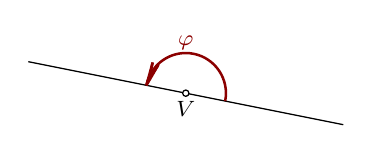
\begin{tikzpicture}
                        % \clip (0,0) rectangle (14.000000,10.000000);
                        {\footnotesize

                        % Drawing line V h
                        \draw [line width=0.016cm] (1.000000,2.000000) -- (2.960777,1.607845);%
                        \draw [line width=0.016cm] (3.039223,1.592155) -- (5.000000,1.200000);%

                        % Marking point V by circle
                        \draw [line width=0.016cm] (3.000000,1.600000) circle (0.040000);%
                        \draw (3.000000,1.600000) node [anchor=north] { $V$ };%

                        % Changing color 139 0 0
                        \definecolor{r139g0b0}{rgb}{0.545098,0.000000,0.000000}%
                        \color{r139g0b0}% 

                        % Drawing arc V h 180.00
                        \draw [line width=0.032cm] (3.500000,1.500000) -- (3.500534,1.502706) arc (349:360:0.509902 and 0.509902) --(3.509902,1.600000) arc (0:168:0.509902 and 0.509902) -- (2.500000,1.700000);%

                        % Marking point \varphi
                        \draw (3.000000,2.050000) node [anchor=south] { $\varphi$ };%

                        % Drawing arrow C A 1.00
                        \draw [line width=0.032cm] (2.651137,1.959148) -- (2.500000,1.700000);%
                        \draw [line width=0.032cm] (2.651137,1.959148) -- (2.538342,1.791430);%
                        \draw [line width=0.032cm] (2.578914,1.989435) -- (2.500000,1.700000);%
                        \draw [line width=0.032cm] (2.578914,1.989435) -- (2.538342,1.791430);%
                        \color{black}
                        }
                    \end{tikzpicture}
                \end{figure}
            \end{alertblock}

            \begin{alertblock}{Definicija}
                Če se poltraka na isti premici prekrivata, določata \textbf{polni kot} ali \textbf{ničelni kot}.

                \begin{figure}[H]
                    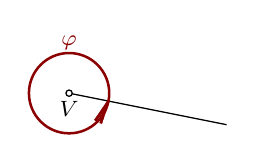
\begin{tikzpicture}
                        % \clip (0,0) rectangle (14.000000,10.000000);
                        {\footnotesize

                        % Drawing line V h
                        % \draw [line width=0.016cm] (1.000000,2.000000) -- (2.960777,1.607845);%
                        \draw [line width=0.016cm] (3.039223,1.592155) -- (5.000000,1.200000);%

                        % Marking point V by circle
                        \draw [line width=0.016cm] (3.000000,1.600000) circle (0.040000);%
                        \draw (3.000000,1.600000) node [anchor=north] { $V$ };%

                        % Changing color 139 0 0
                        \definecolor{r139g0b0}{rgb}{0.545098,0.000000,0.000000}%
                        \color{r139g0b0}% 

                        % Drawing arc V h 360.00
                        \draw [line width=0.032cm] (3.000000,1.600000) circle (0.509902);%

                        % Marking point \varphi
                        \draw (3.000000,2.050000) node [anchor=south] { $\varphi$ };%

                        % Drawing arrow k h 1.00
                        \draw [line width=0.032cm] (3.331960,1.251479) -- (3.500000,1.500000);%
                        \draw [line width=0.032cm] (3.331960,1.251479) -- (3.455661,1.411322);%
                        \draw [line width=0.032cm] (3.402008,1.216456) -- (3.500000,1.500000);%
                        \draw [line width=0.032cm] (3.402008,1.216456) -- (3.455661,1.411322);%
                        \color{black}
                        }
                    \end{tikzpicture} ~~~~~
                    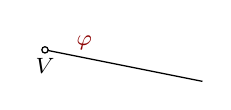
\begin{tikzpicture}
                        % \clip (0,0) rectangle (14.000000,10.000000);
                        {\footnotesize

                        % Drawing line V h
                        % \draw [line width=0.016cm] (1.000000,2.000000) -- (2.960777,1.607845);%
                        \draw [line width=0.016cm] (3.039223,1.592155) -- (5.000000,1.200000);%

                        % Marking point V by circle
                        \draw [line width=0.016cm] (3.000000,1.600000) circle (0.040000);%
                        \draw (3.000000,1.600000) node [anchor=north] { $V$ };%

                        % Changing color 139 0 0
                        \definecolor{r139g0b0}{rgb}{0.545098,0.000000,0.000000}%
                        \color{r139g0b0}% 

                        % Marking point \varphi
                        \draw (3.500000,1.500000) node [anchor=south] { $\varphi$ };%
                        \color{black}
                        }
                    \end{tikzpicture}
                \end{figure}

            \end{alertblock}
        \end{frame}


        \begin{frame}
            \begin{alertblock}{Definicija}
                Kota s skupnim vrhom, ki imata en skupen krak, presek njunih notranjosti pa je prazen, sta \textbf{sosedna kota}.

                \begin{figure}[H]
                    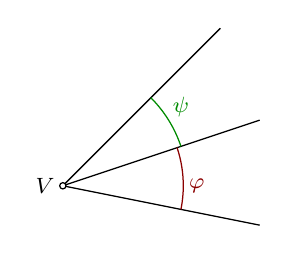
\begin{tikzpicture}
                        % \clip (0,0) rectangle (14.000000,10.000000);
                        {\footnotesize

                        % Drawing line V P
                        \draw [line width=0.016cm] (4.000000,1.000000) -- (1.539223,1.492155);%
                        % \draw [line width=0.016cm] (1.460777,1.507845) -- (1.000000,1.600000);%

                        % Drawing line V Q
                        % \draw [line width=0.016cm] (1.000000,1.333333) -- (1.462053,1.487351);%
                        \draw [line width=0.016cm] (1.537947,1.512649) -- (4.000000,2.333333);%

                        % Drawing line V R
                        % \draw [line width=0.016cm] (1.000000,1.000000) -- (1.471716,1.471716);%
                        \draw [line width=0.016cm] (1.528284,1.528284) -- (3.500000,3.500000);%

                        % Marking point V by circle
                        \draw [line width=0.016cm] (1.500000,1.500000) circle (0.040000);%
                        \draw (1.500000,1.500000) node [anchor=east] { $V$ };%

                        % Changing color 139 0 0
                        \definecolor{r139g0b0}{rgb}{0.545098,0.000000,0.000000}%
                        \color{r139g0b0}% 

                        % Drawing arc V P 29.74
                        \draw [line width=0.016cm] (3.000000,1.200000) -- (3.001601,1.208118) arc (349:360:1.529706 and 1.529706) --(3.029706,1.500000) arc (0:18:1.529706 and 1.529706) -- (2.951206,1.983735);%

                        % Marking point \varphi
                        \draw (3.200000,1.500000) node  { $\varphi$ };%

                        % Changing color 0 139 0
                        \definecolor{r0g139b0}{rgb}{0.000000,0.545098,0.000000}%
                        \color{r0g139b0}% 

                        % Drawing arc V Q 26.57
                        \draw [line width=0.016cm] (3.000000,2.000000) -- (2.994996,2.014768) arc (19:45:1.581139 and 1.581139);%

                        % Marking point \psi
                        \draw (3.000000,2.500000) node  { $\psi$ };%
                        \color{black}
                        }
                    \end{tikzpicture}
                \end{figure}
            % \end{alertblock}

            % \begin{alertblock}{Definicija}
                Sosedna kota, katerih kraka, ki  nista skupna, ležita na isti premici, sta \textbf{sokota}.
                
                \begin{figure}[H]
                    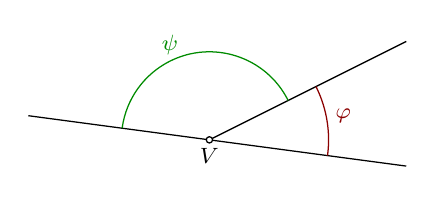
\begin{tikzpicture}
                        % \clip (0,0) rectangle (14.000000,10.000000);
                        {\footnotesize

                        % Drawing line V P
                        \draw [line width=0.016cm] (1.200000,1.806667) -- (3.460351,1.505287);%
                        \draw [line width=0.016cm] (3.539649,1.494713) -- (6.000000,1.166667);%

                        % Drawing line V Q
                        % \draw [line width=0.016cm] (2.700000,1.100000) -- (3.464223,1.482111);%
                        \draw [line width=0.016cm] (3.535777,1.517889) -- (6.000000,2.750000);%

                        % Marking point V by circle
                        \draw [line width=0.016cm] (3.500000,1.500000) circle (0.040000);%
                        \draw (3.500000,1.500000) node [anchor=north] { $V$ };%

                        % Changing color 139 0 0
                        \definecolor{r139g0b0}{rgb}{0.545098,0.000000,0.000000}%
                        \color{r139g0b0}% 

                        % Drawing arc V P 34.16
                        \draw [line width=0.016cm] (5.000000,1.300000) -- (5.001995,1.315578) arc (353:360:1.513275 and 1.513275) --(5.013275,1.500000) arc (0:26:1.513275 and 1.513275) -- (4.853514,2.176757);%

                        % Marking point \varphi
                        \draw (5.200000,1.800000) node  { $\varphi$ };%

                        % Changing color 0 139 0
                        \definecolor{r0g139b0}{rgb}{0.000000,0.545098,0.000000}%
                        \color{r0g139b0}% 

                        % Drawing arc V Q 145.84
                        \draw [line width=0.016cm] (4.500000,2.000000) -- (4.496176,2.007577) arc (27:172:1.118034 and 1.118034) -- (2.391774,1.647764);%

                        % Marking point \psi
                        \draw (3.000000,2.700000) node  { $\psi$ };%
                        \color{black}
                        }
                    \end{tikzpicture}
                \end{figure}
            \end{alertblock}

        \end{frame}


        \begin{frame}
            \begin{alertblock}{Definicija}
                Tri nekolinearne točke $A$, $B$ in $C$ določajo \textbf{trikotnik} $\triangle ABC$.
                Točke $A$, $B$ in $C$ so \textbf{oglišča} trikotnika, daljice $AB$, $BC$ in $AC$ so njegove \textbf{stranice}.

            \begin{figure}
                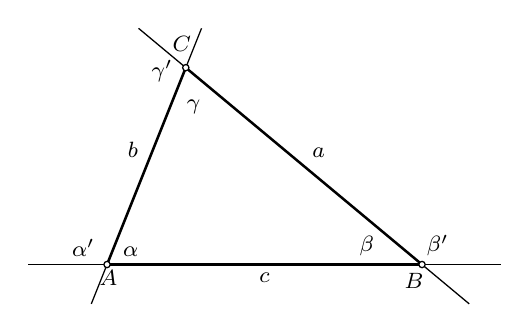
\begin{tikzpicture}
                    % \clip (0,0) rectangle (14.000000,10.000000);
                    {\footnotesize
                    
                    % Marking point A by circle
                    \draw<2-> [line width=0.016cm] (2.000000,1.500000) circle (0.040000);%
                    \draw<2-> (1.800000,1.530000) node [anchor=north west] { $A$ };%
                    
                    % Marking point B by circle
                    \draw<2-> [line width=0.016cm] (6.000000,1.500000) circle (0.040000);%
                    \draw<2-> (5.900000,1.500000) node [anchor=north] { $B$ };%
                    
                    % Marking point C by circle
                    \draw<2-> [line width=0.016cm] (3.000000,4.000000) circle (0.040000);%
                    \draw<2-> (2.950000,4.100000) node [anchor=south] { $C$ };%
                    
                    % Drawing line A B
                    \draw<4-> [line width=0.016cm] (1.000000,1.500000) -- (1.960000,1.500000);%
                    \draw<4-> [line width=0.016cm] (2.040000,1.500000) -- (5.960000,1.500000);%
                    \draw<4-> [line width=0.016cm] (6.040000,1.500000) -- (7.000000,1.500000);%
                    
                    % Drawing line B C
                    \draw<4-> [line width=0.016cm] (6.600000,1.000000) -- (6.030729,1.474393);%
                    \draw<4-> [line width=0.016cm] (5.969271,1.525607) -- (3.030729,3.974393);%
                    \draw<4-> [line width=0.016cm] (2.969271,4.025607) -- (2.400000,4.500000);%
                    
                    % Drawing line A C
                    \draw<4-> [line width=0.016cm] (1.800000,1.000000) -- (1.985144,1.462861);%
                    \draw<4-> [line width=0.016cm] (2.014856,1.537139) -- (2.985144,3.962861);%
                    \draw<4-> [line width=0.016cm] (3.014856,4.037139) -- (3.200000,4.500000);%
                    
                    % Marking point c
                    \draw<2-> (4.000000,1.500000) node [anchor=north] { $c$ };%
                    
                    % Marking point a
                    \draw<2-> (4.500000,2.750000) node [anchor=south west] { $a$ };%
                    
                    % Marking point b
                    \draw<2-> (2.500000,2.750000) node [anchor=south east] { $b$ };%
                    
                    % Marking point \gamma
                    \draw<3-> (3.100000,3.700000) node [anchor=north] { $\gamma$ };%
                    
                    % Marking point \gamma'
                    \draw<4-> (2.700000,4.200000) node [anchor=north] { $\gamma'$ };%
                    
                    % Marking point \beta
                    \draw<3-> (5.300000,1.500000) node [anchor=south] { $\beta$ };%
                    
                    % Marking point \beta'
                    \draw<4-> (6.200000,1.500000) node [anchor=south] { $\beta'$ };%
                    
                    % Marking point \alpha
                    \draw<3-> (2.300000,1.500000) node [anchor=south] { $\alpha$ };%
                    
                    % Marking point \alpha'
                    \draw<4-> (1.700000,1.500000) node [anchor=south] { $\alpha'$ };%
                    
                    % Drawing segment A B
                    \draw<2-> [line width=0.032cm] (2.040000,1.500000) -- (5.960000,1.500000);%
                    
                    % Drawing segment B C
                    \draw<2-> [line width=0.032cm] (5.969271,1.525607) -- (3.030729,3.974393);%
                    
                    % Drawing segment A C
                    \draw<2-> [line width=0.032cm] (2.014856,1.537139) -- (2.985144,3.962861);%
                    }
                \end{tikzpicture}
            \end{figure}

                Koti $\alpha$, $\beta$ in $\gamma$ so \textbf{notranji koti}, 
                njihovi sokoti $\alpha'$, $\beta'$ in $\gamma'$ pa so \textbf{zunanji koti} trikotnika.

            \end{alertblock}

            \begin{block}{}
                Trikotnik je \textbf{pozitivno orientiran}, če si njegova oglišča sledijo v nasprotni smeri vrtenja urnega kazalca; 
                če si sledijo v smeri vrtenja urnega kazalca, pa je \textbf{negativno orientiran}.
            \end{block}
        \end{frame}


        \begin{frame}
            \begin{alertblock}{Definicija}
                Točke $A_1, A_2, A_3, \dots, A_n$ v ravnini, od katerih nobene zaporedne tri niso kolinearne, določajo \textbf{$n$-kotnik}.

                Točke $A_1, A_2, A_3, \dots, A_n$ so \textbf{oglišča} $n$-kotnika;
                daljice, ki povezujejo sosedni oglišči, $A_1A_2, A_2A_3, \dots, A_nA_1$ so \textbf{stranice} $n$-kotnika;
                daljice, ki povezujejo po dve nesosedni oglišči, pa so \textbf{diagonale} $n$-kotnika.
            \end{alertblock}

            \begin{block}{}
                Poljuben $n$-kotnika ima $$\dfrac{n(n-3)}{2}$$ diagonal -- iz vsakega od $n$ oglišč gre $n-3$ diagonal, vsaka pa je šteta dvakrat.
            \end{block}

            \begin{block}{}
                Če za vsako nosilko stranice $n$-kotnika velja, da preostala oglišča ležijo na isti strani te nosilke, je $n$-kotnik \textbf{konveksen}.
            \end{block}
        \end{frame}




        %%%%% naloge

        \begin{frame}

            \only<2->{\begin{exampleblock}{Naloga}
                Izračunajte število diagonal: $17$-kotnika, $31$-kotnika in $28$-kotnika.                
            \end{exampleblock}}

            \only<3->{\begin{exampleblock}{Naloga}
                Ugotovite, ali obstaja $n$-kotnik, ki ima desetino toliko diagonal kot $28$-kotnik.
                Če obstaja, izračunajte, koliko stranic ima.
            \end{exampleblock}}   
            
            \only<4->{\begin{exampleblock}{Naloga}
                Kateri $n$-kotnik ima štirikrat toliko diagonal kot stranic?
            \end{exampleblock}}
        
            \only<5->{\begin{exampleblock}{Naloga}
                Izračunajte, kateri $n$-kotnik ima: $104$ diagonale, $230$ diagonal, $2n-5$ diagonal.
            \end{exampleblock}}

            \only<6->{\begin{exampleblock}{Naloga}
                Pokažite, da ne obstaja $n$-kotnik, ki ima $13$ diagonal.  
            \end{exampleblock}}
            
        \end{frame}


        \begin{frame}

            \only<2->{\begin{exampleblock}{Naloga}
                Za vsako od spodnjih izjav ugotovite, ali je pravilna ali nepravilna.
                \begin{itemize}
                    \item Tri različne točke, so vedno nekolinearne.
                    \item Petkotnik ima enako število diagonal in stranic.
                    \item Štiri različne premice se sekajo v največ $4$ različnih točkah.
                    \item Skozi štiri kolinearne točke gredo tri različne premice.
                    \item Vzporedni premici imata lahko neskončno mnogo skupnih točk.
                \end{itemize}
            \end{exampleblock}}

            \only<3->{\begin{exampleblock}{Naloga}
                Pokažite, da je število diagonal $25$-kotnika večkratnik števila njegovih stranic.
            \end{exampleblock}}

            \only<4->{\begin{exampleblock}{Naloga}
                Vsota števila stranic in diagonal $n$-kotnika je $105$? Kateri $n$-kotnik je to?
            \end{exampleblock}}

        \end{frame}


        \begin{frame}

            \only<2->{\begin{exampleblock}{Naloga}
                Izračunajte, kateri $n$-kotnik ima toliko diagonal kot stranic.
            \end{exampleblock}}

            \only<3->{\begin{exampleblock}{Naloga}
                Člani filatelističnega društva so se domenili, da si bodo za praznike spet pošiljali voščilnice po klasični pošti.
                Ko so se dobili po novem letu, so prinesli vse voščilnice in jih našteli $132$.
                Izračunajte, koliko članov društva, si je medseboj poslalo voščilnice.                
            \end{exampleblock}}


        \end{frame}





%%%%%%%%%%%%%%%%%%%%%%%%%%%%%%%%%%%%%
    \subsection{Skladnost in merjenje}

        \begin{frame}
            \frametitle{Skladnost}

            \begin{alertblock}{Definicija}
                Dva lika $L$ in $L'$ sta \textbf{skladna}, če lahko lik $L$ prenesemo na lik $L'$ tako,
                da se popolnoma prekrijeta.

                Znak za skladnost je $\cong$.
            \end{alertblock}

            \begin{block}{}
                \textbf{Skladnost} je v množici ravninskih likov \textit{ekvivalenčna relacija}, saj je:
                \begin{itemize}
                    \item \textit{refleksivna}: $L\cong L'$ -- vsaka množica je skladna sama s seboj;
                    \item \textit{simetrična}: $L\cong L' \Rightarrow L'\cong L$ -- če je prva množica skladna z drugo, je tudi druga skladna s prvo;
                    \item \textit{tranzitivna}: $L\cong L' \land L'\cong L'' \rightarrow L\cong L''$ -- če je prva množica skladna z drugo in druga skladna s tretjo, 
                            je tudi prva množica skladna s tretjo množico.
                \end{itemize}
            \end{block}
        \end{frame}


        \begin{frame}
            \begin{alertblock}{Definicija}
                Kot, ki je skladen s svojim kotom, je \textbf{pravi kot}.

                \begin{figure}[H]
                    \begin{tikzpicture}
                    % \clip (0,0) rectangle (14.000000,10.000000);
                    {\footnotesize

                    % Drawing line V A
                    \draw [line width=0.016cm] (1.000000,1.500000) -- (2.960000,1.500000);%
                    \draw [line width=0.016cm] (3.040000,1.500000) -- (5.000000,1.500000);%

                    % Drawing line V B
                    % \draw [line width=0.016cm] (3.000000,1.000000) -- (3.000000,1.460000);%
                    \draw [line width=0.016cm] (3.000000,1.540000) -- (3.000000,3.500000);%

                    % Marking point V by circle
                    \draw [line width=0.016cm] (3.000000,1.500000) circle (0.040000);%

                    % Changing color 139 0 0
                    \definecolor{r139g0b0}{rgb}{0.545098,0.000000,0.000000}%
                    \color{r139g0b0}% 

                    % Drawing arc V A 90.00
                    \draw [line width=0.032cm] (3.800000,1.500000) arc (360:360:0.800000 and 0.800000) --(3.800000,1.500000) arc (0:90:0.800000 and 0.800000);%

                    % Changing color 0 139 0
                    \definecolor{r0g139b0}{rgb}{0.000000,0.545098,0.000000}%
                    \color{r0g139b0}% 

                    % Drawing arc V B 90.00
                    \draw [line width=0.032cm] (3.000000,2.200000) arc (90:180:0.700000 and 0.700000);%
                    \color{black}
                    }
                    \end{tikzpicture}

                \end{figure}
                
            \end{alertblock}

            \begin{block}{}
                Če si kraka sledita v nasprotni smeri vrtenja urnega kazalca, je \textbf{orientacija kota pozitivna}, 
                če pa si sledita v smeri vrtenja urnega kazalca, pa je \textbf{orientacija kota negativna}.

                \begin{figure}[H]
                    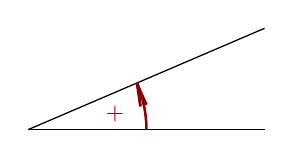
\begin{tikzpicture}
                    % \clip (0,0) rectangle (14.000000,10.000000);
                    {\footnotesize

                    % Drawing segment A b
                    \draw [line width=0.016cm] (1.500000,1.500000) -- (4.500000,1.500000);%

                    % Drawing segment A C
                    \draw [line width=0.016cm] (1.500000,1.500000) -- (4.500000,2.785714);%

                    % Changing color 139 0 0
                    \definecolor{r139g0b0}{rgb}{0.545098,0.000000,0.000000}%
                    \color{r139g0b0}% 

                    % Drawing arc A B 23.20
                    \draw [line width=0.032cm] (3.000000,1.500000) arc (360:360:1.500000 and 1.500000) --(3.000000,1.500000) arc (0:23:1.500000 and 1.500000) -- (2.878718,2.090879);%

                    % Drawing arrow Bb U 1.00
                    \draw [line width=0.032cm] (2.923918,1.794304) -- (2.878718,2.090879);%
                    \draw [line width=0.032cm] (2.923918,1.794304) -- (2.906321,1.995655);%
                    \draw [line width=0.032cm] (2.999137,1.816108) -- (2.878718,2.090879);%
                    \draw [line width=0.032cm] (2.999137,1.816108) -- (2.906321,1.995655);%

                    % Marking point +
                    \draw (2.600000,1.700000) node  { $+$ };%
                    \color{black}
                    }
                    \end{tikzpicture} ~~~~~
                    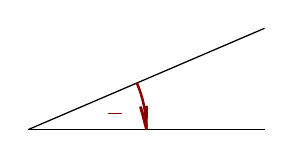
\begin{tikzpicture}
                    % \clip (0,0) rectangle (14.000000,10.000000);
                    {\footnotesize

                    % Drawing segment A b
                    \draw [line width=0.016cm] (1.500000,1.500000) -- (4.500000,1.500000);%

                    % Drawing segment A C
                    \draw [line width=0.016cm] (1.500000,1.500000) -- (4.500000,2.785714);%

                    % Changing color 139 0 0
                    \definecolor{r139g0b0}{rgb}{0.545098,0.000000,0.000000}%
                    \color{r139g0b0}% 

                    % Drawing arc A B 23.20
                    \draw [line width=0.032cm] (3.000000,1.500000) arc (360:360:1.500000 and 1.500000) --(3.000000,1.500000) arc (0:23:1.500000 and 1.500000) -- (2.878718,2.090879);%

                    % Drawing arrow Bb B 1.00
                    \draw [line width=0.032cm] (3.001963,1.799994) -- (3.000000,1.500000);%
                    \draw [line width=0.032cm] (3.001963,1.799994) -- (2.987703,1.598379);%
                    \draw [line width=0.032cm] (2.924252,1.790280) -- (3.000000,1.500000);%
                    \draw [line width=0.032cm] (2.924252,1.790280) -- (2.987703,1.598379);%

                    % Marking point -
                    \draw (2.600000,1.700000) node  { $-$ };%
                    \color{black}
                    }
                    \end{tikzpicture}
                \end{figure}
            \end{block}
        \end{frame}

        \begin{frame}
            \frametitle{Merjenje}

            \vskip-1.5em
            \begin{block}{}
                Daljici $AB$ in $CD$, ki nista skladni, lahko premaknemo na poljubni premici tako,
                da levi krajišči sovpadata in da eno od desnih krajišč, npr. $D$ leži med $A$ in $B$.
                V tem primeru je daljica $AB$ \textbf{daljša} od daljice $CD$ oziroma je daljica $CD$ \textbf{krajša} od daljice $AB$.
            \end{block}

            \begin{alertblock}{Arhimedov aksiom}
                Obstaja tako naravno število $n$, pri katerem je vsota $n$ krajših daljic $CD$ daljša od daljice $AB$,
                vsota $n-1$ krajših daljic $CD$ pa je kvečjemu skladna z daljico $AB$.
                % $$n\cdot |CD|>|AB| \quad \quad (n-1)\cdot |CD|\leq |AB|$$

                \begin{figure}[H]
                    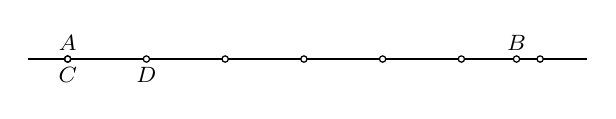
\begin{tikzpicture}
                    % \clip (0,0) rectangle (14.000000,10.000000);
                    {\footnotesize

                    % Drawing line A B
                    \draw [line width=0.016cm] (1.000000,1.500000) -- (1.460000,1.500000);%
                    \draw [line width=0.016cm] (1.540000,1.500000) -- (2.460000,1.500000);%
                    \draw [line width=0.016cm] (2.540000,1.500000) -- (3.460000,1.500000);%
                    \draw [line width=0.016cm] (3.540000,1.500000) -- (4.460000,1.500000);%
                    \draw [line width=0.016cm] (4.540000,1.500000) -- (5.460000,1.500000);%
                    \draw [line width=0.016cm] (5.540000,1.500000) -- (6.460000,1.500000);%
                    \draw [line width=0.016cm] (6.540000,1.500000) -- (7.160000,1.500000);%
                    \draw [line width=0.016cm] (7.240000,1.500000) -- (7.460000,1.500000);%
                    \draw [line width=0.016cm] (7.540000,1.500000) -- (8.100000,1.500000);%

                    % Marking point A by circle
                    \draw [line width=0.016cm] (1.500000,1.500000) circle (0.040000);%
                    \draw (1.500000,1.500000) node [anchor=south] { $A$ };%

                    % Marking point B by circle
                    \draw [line width=0.016cm] (7.200000,1.500000) circle (0.040000);%
                    \draw (7.200000,1.500000) node [anchor=south] { $B$ };%

                    % Marking point C by circle
                    \draw [line width=0.016cm] (1.500000,1.500000) circle (0.040000);%
                    \draw (1.500000,1.500000) node [anchor=north] { $C$ };%

                    % Marking point D by circle
                    \draw [line width=0.016cm] (2.500000,1.500000) circle (0.040000);%
                    \draw (2.500000,1.500000) node [anchor=north] { $D$ };%

                    % Marking point E by circle
                    \draw [line width=0.016cm] (3.500000,1.500000) circle (0.040000);%

                    % Marking point F by circle
                    \draw [line width=0.016cm] (4.500000,1.500000) circle (0.040000);%

                    % Marking point G by circle
                    \draw [line width=0.016cm] (5.500000,1.500000) circle (0.040000);%

                    % Marking point H by circle
                    \draw [line width=0.016cm] (6.500000,1.500000) circle (0.040000);%

                    % Marking point I by circle
                    \draw [line width=0.016cm] (7.500000,1.500000) circle (0.040000);%
                    }
                    \end{tikzpicture}
                \end{figure}
            \end{alertblock}

            % \begin{block}{}
            %     Daljico $CD$, s katero smo izmerili daljico $AB$, imenujemo \textbf{enotska daljica}.
            %     Tako smo daljici $AB$ priredili natančno določeno število -- \textbf{dolžino} daljice $AB$ oziroma \textbf{razdaljo} točk $A$ in $B$.
            %     $$ |AB|=d(A,B)$$
            % \end{block}
            \begin{block}{}
                Daljico $CD$ imenujemo \textbf{enotska daljica}.
                Daljici $AB$ smo priredili natančno določeno število -- \textbf{dolžino} daljice $AB$ oziroma \textbf{razdaljo} točk $A$ in $B$.
                \vskip-1em
                $$ |AB|=d(A,B)$$
            \end{block}

        \end{frame}


        \begin{frame}
            \begin{alertblock}{Aksiom}
                Če je $AB$ poljubna daljica, $A'$ pa točka na poljubnem poltraku, obstaja na tem poltraku natančno določena točka $B'$,
                da je daljica $A'B'$ skladna z daljico $AB$.
                \vskip-1em
                $$A'B'\cong AB$$
            \end{alertblock}

            \begin{block}{Izrek}
                Skladni daljici imata enako dolžino.
                % $$|A'B'|=|AB|$$
            \end{block}

            \begin{alertblock}{Aksiom}
                Naj daljici $AB$ in $BC$ ležita na isti premici in naj imata skupno le točko $B$.
                Daljici $A'B'$ in $B'C'$ naj ležita na tej ali neki drugi premici in naj imata skupno točko $B'$.
                Če velja $AB\cong A'B'$ in $BC\cong B'C'$, potem velja tudi $AC\cong A'C'$.
            \end{alertblock}

            \begin{block}{Izrek}
                Dolžina vsote daljic je enaka vsoti dolžin posameznih daljic.
            \end{block}
        \end{frame}


        \begin{frame}
            \frametitle{Enote}

            \vskip-1em
            \begin{block}{}
                Osnovna enota za merjenje dolžine je \textbf{meter}.

                Iz nje izpeljane enote pa so \textit{decimeter}, \textit{centimeter}, \textit{milimeter}, \textit{kilometer} itd.
                $$ 1~m=10~dm=100~cm=1000~mm$$  $$1~km=1000~m$$ 
            \end{block}

            \begin{block}{}
                Enota za merjenje kotov je \textbf{kotna stopinja} -- velikost $\dfrac{1}{360}$ polnega kota.
                
                Izpeljani enoti sta \textit{(kotna) minuta} in \textit{(kotna) sekunda}.
                $$1^\circ=60'=3600''$$ 
            \end{block}

            \begin{block}{}
                Velikost kota nič je $0^\circ$, pravega kota je $90^\circ$, iztegnjenega kota je $180^\circ$, polnega kota pa je $360^\circ$.
            \end{block}
        \end{frame}


        \begin{frame}
            \begin{alertblock}{Definicija}
                Kota $\varphi$ in $\psi$, katerih vsota meri $180^\circ$, sta \textbf{suplementarna kota}.

                \begin{figure}[H]
                    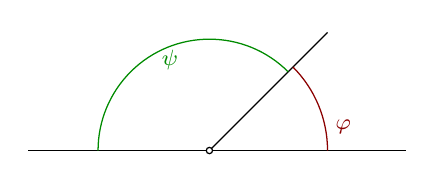
\begin{tikzpicture}
                    % \clip (0,0) rectangle (14.000000,10.000000);
                    {\footnotesize

                    % Drawing line V P
                    \draw [line width=0.016cm] (1.200000,1.500000) -- (3.460000,1.500000);%
                    \draw [line width=0.016cm] (3.540000,1.500000) -- (6.000000,1.500000);%

                    % Drawing line V Q
                    % \draw [line width=0.016cm] (3.100000,1.100000) -- (3.471716,1.471716);%
                    \draw [line width=0.016cm] (3.528284,1.528284) -- (5.000000,3.000000);%

                    % Marking point V by circle
                    \draw [line width=0.016cm] (3.500000,1.500000) circle (0.040000);%

                    % Changing color 139 0 0
                    \definecolor{r139g0b0}{rgb}{0.545098,0.000000,0.000000}%
                    \color{r139g0b0}% 

                    % Drawing arc V P 45.00
                    \draw [line width=0.016cm] (5.000000,1.500000) arc (360:360:1.500000 and 1.500000) --(5.000000,1.500000) arc (0:45:1.500000 and 1.500000);%

                    % Marking point \varphi
                    \draw (5.200000,1.80000) node  { $\varphi$ };%

                    % Changing color 0 139 0
                    \definecolor{r0g139b0}{rgb}{0.000000,0.545098,0.000000}%
                    \color{r0g139b0}% 

                    % Drawing arc V Q 135.00
                    \draw [line width=0.016cm] (4.500000,2.500000) arc (45:180:1.414214 and 1.414214);%

                    % Marking point \psi
                    \draw (3.000000,2.650000) node  { $\psi$ };%
                    \color{black}
                    }
                    \end{tikzpicture}
                \end{figure}
            \end{alertblock}

                        
            \begin{alertblock}{Definicija}
                Kota $\varphi$ in $\psi$, katerih vsota meri $90^\circ$, sta \textbf{komplementarna kota}.

                \begin{figure}[H]
                    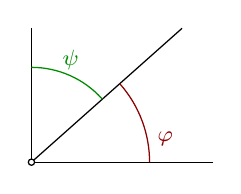
\begin{tikzpicture}
                    % \clip (0,0) rectangle (14.000000,10.000000);
                    {\footnotesize

                    % Drawing line V P
                    % \draw [line width=0.016cm] (2.800000,1.500000) -- (3.460000,1.500000);%
                    \draw [line width=0.016cm] (3.540000,1.500000) -- (5.800000,1.500000);%

                    % Drawing line V Q
                    % \draw [line width=0.016cm] (3.050000,1.100000) -- (3.470104,1.473425);%
                    \draw [line width=0.016cm] (3.529896,1.526575) -- (5.412500,3.200000);%

                    % Drawing line V R
                    % \draw [line width=0.016cm] (3.500000,1.100000) -- (3.500000,1.460000);%
                    \draw [line width=0.016cm] (3.500000,1.540000) -- (3.500000,3.200000);%

                    % Marking point V by circle
                    \draw [line width=0.016cm] (3.500000,1.500000) circle (0.040000);%

                    % Changing color 139 0 0
                    \definecolor{r139g0b0}{rgb}{0.545098,0.000000,0.000000}%
                    \color{r139g0b0}% 

                    % Drawing arc V P 41.63
                    \draw [line width=0.016cm] (5.000000,1.500000) arc (360:360:1.500000 and 1.500000) --(5.000000,1.500000) arc (0:41:1.500000 and 1.500000) -- (4.621114,2.496546);%

                    % Marking point \varphi
                    \draw (5.200000,1.800000) node  { $\varphi$ };%

                    % Changing color 0 139 0
                    \definecolor{r0g139b0}{rgb}{0.000000,0.545098,0.000000}%
                    \color{r0g139b0}% 

                    % Drawing arc V Q 48.37
                    \draw [line width=0.016cm] (4.400000,2.300000) -- (4.394865,2.305740) arc (42:90:1.204159 and 1.204159);%

                    % Marking point \psi
                    \draw (4.000000,2.800000) node  { $\psi$ };%
                    \color{black}
                    }
                    \end{tikzpicture}
                \end{figure}
            \end{alertblock}

            \begin{block}{}
                Sokota sta vedno suplementarna kota.
            \end{block}
        \end{frame}


        \begin{frame}
            \frametitle{Skladnost trikotnikov}

            \vskip-1em
            \begin{alertblock}{Definicija}
                Dva trikotnika sta \textbf{skladna}, če imata paroma skladne vse stranice in tem stranicam nasprotne kote.
            \end{alertblock}

            \begin{alertblock}{Aksiom}
                Dva trikotnika sta skladna, če se ujemata v dveh stranicah in v vmesnem kotu.
            \end{alertblock}

            \begin{block}{Izrek}
                Trikotnika $\triangle ABC$ in $\triangle A'B'C'$ sta skladna, če se ujemata:
                \begin{enumerate}
                    \item v vseh treh stranicah;
                    \item v eni stranici in obeh priležnih kotih;
                    \item v dveh stranicah in kotu, ki leži nasproti daljši od obeh stranic.
                \end{enumerate}
            \end{block}
        \end{frame}



%%%% naloge



        \begin{frame}

            \only<2->{\begin{exampleblock}{Naloga}
                Izračunajte dolžino daljice, če ena polovica meri $2x-7$ enot, druga polovica pa $x+8$ enot.
            \end{exampleblock}}

            \only<3->{\begin{exampleblock}{Naloga}
                Izračunaj dolžino $x$ daljice $AB$, če je točka $S$ njeno razpolovišče, točka $R$ pa razpolovišče daljice $SB$ in je $\lvert SR \rvert = \dfrac{x}{3}-1$.
            \end{exampleblock}}

            \only<4->{\begin{exampleblock}{Naloga}
                Izračunajte velikosti kotov $\alpha$ in $\beta$, če je $\alpha=\beta$.
                Podatke razberite s skice.

                \begin{figure}
                    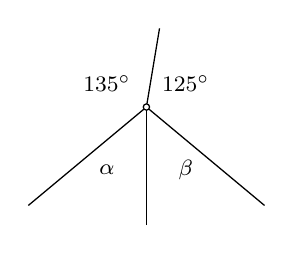
\begin{tikzpicture}
                        % \clip (0,0) rectangle (14.000000,10.000000);
                        {\footnotesize

                        % Marking point A by circle
                        \draw [line width=0.016cm] (3.000000,3.000000) circle (0.040000);%

                        % Drawing segment A B
                        \draw [line width=0.016cm] (3.000000,1.500000) -- (3.000000,2.960000);%

                        % Drawing segment A C
                        \draw [line width=0.016cm] (3.030729,2.974393) -- (4.500000,1.750000);%

                        % Drawing segment A D
                        \draw [line width=0.016cm] (2.969271,2.974393) -- (1.500000,1.750000);%

                        % Drawing segment A E
                        \draw [line width=0.016cm] (3.006576,3.039456) -- (3.166667,4.000000);%

                        % Marking point \beta
                        \draw (3.500000,2.200000) node  { $\beta$ };%

                        % Marking point \alpha
                        \draw (2.500000,2.200000) node  { $\alpha$ };%

                        % Marking point {125^\circ}
                        \draw (3.500000,3.300000) node  { ${125^\circ}$ };%

                        % Marking point {135^\circ}
                        \draw (2.500000,3.300000) node  { ${135^\circ}$ };%
                        }
                    \end{tikzpicture}

                \end{figure}
            \end{exampleblock}}


        \end{frame}


        \begin{frame}
            % \vskip-0.5em
            % \begin{columns}
            % \column{0.33\textwidth}   
            \only<2->{\begin{exampleblock}{Naloga}
                Iz podatkov na skici izračunajte neznano velikost kota $x$.

                \begin{figure}
                    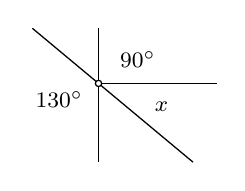
\begin{tikzpicture}
                        % \clip (0,0) rectangle (14.000000,10.000000);
                        {\footnotesize

                        % Marking point A by circle
                        \draw [line width=0.016cm] (3.000000,3.000000) circle (0.040000);%

                        % Drawing line A B
                        \draw [line width=0.016cm] (3.000000,2.000000) -- (3.000000,2.960000);%
                        \draw [line width=0.016cm] (3.000000,3.040000) -- (3.000000,3.700000);%

                        % Drawing line A C
                        \draw [line width=0.016cm] (4.200000,2.000000) -- (3.030729,2.974393);%
                        \draw [line width=0.016cm] (2.969271,3.025607) -- (2.160000,3.700000);%

                        % Drawing segment A E
                        \draw [line width=0.016cm] (3.040000,3.000000) -- (4.500000,3.000000);%

                        % Marking point x
                        \draw (3.800000,2.700000) node  { $x$ };%

                        % Marking point {90^\circ}
                        \draw (3.500000,3.300000) node  { ${90^\circ}$ };%

                        % Marking point {130^\circ}
                        \draw (2.500000,2.800000) node  { ${130^\circ}$ };%
                        }
                    \end{tikzpicture}

                \end{figure}
            \end{exampleblock}}

            % \column{0.63\textwidth}   
            \only<3->{\begin{exampleblock}{Naloga}
                Izračunajte velikosti kotov $\angle AVM$ in $\angle FVE$, če poltrak $VM$ obakrat razpolavlja kot.

                \begin{figure}
                    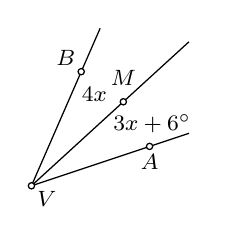
\begin{tikzpicture}
                        % \clip (0,0) rectangle (14.000000,10.000000);
                        {\footnotesize

                        % Marking point V by circle
                        \draw [line width=0.016cm] (1.500000,1.500000) circle (0.040000);%
                        \draw (1.470000,1.530000) node [anchor=north west] { $V$ };%

                        % Marking point A by circle
                        \draw [line width=0.016cm] (3.000000,2.000000) circle (0.040000);%
                        \draw (3.000000,2.000000) node [anchor=north] { $A$ };%

                        % Drawing line V A
                        % \draw [line width=0.016cm] (1.200000,1.400000) -- (1.462053,1.487351);%
                        \draw [line width=0.016cm] (1.537947,1.512649) -- (2.962053,1.987351);%
                        \draw [line width=0.016cm] (3.037947,2.012649) -- (3.500000,2.166667);%

                        % Marking point M by circle
                        \draw [line width=0.016cm] (2.666950,2.566878) circle (0.040000);%
                        \draw (2.666950,2.666878) node [anchor=south] { $M$ };%

                        % Marking point B by circle
                        \draw [line width=0.016cm] (2.132124,2.949283) circle (0.040000);%
                        \draw (2.162124,2.919283) node [anchor=south east] { $B$ };%

                        % Drawing line V B
                        % \draw [line width=0.016cm] (1.369151,1.200000) -- (1.484008,1.463336);%
                        \draw [line width=0.016cm] (1.515992,1.536664) -- (2.116132,2.912618);%
                        \draw [line width=0.016cm] (2.148115,2.985947) -- (2.372326,3.500000);%

                        % Drawing line V M
                        % \draw [line width=0.016cm] (1.200000,1.225727) -- (1.470478,1.473010);%
                        \draw [line width=0.016cm] (1.529522,1.526990) -- (2.637428,2.539888);%
                        \draw [line width=0.016cm] (2.696472,2.593868) -- (3.500000,3.328489);%

                        % Marking point {3x+6^\circ}
                        \draw (3.033475,2.283439) node  { ${3x+6^\circ}$ };%

                        % Marking point {4x}
                        \draw (2.299537,2.658080) node  { ${4x}$ };%
                        }
                    \end{tikzpicture} ~
                    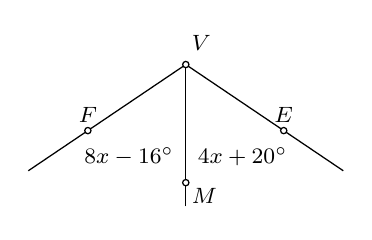
\begin{tikzpicture}
                        % \clip (0,0) rectangle (14.000000,10.000000);
                        {\footnotesize

                        % Marking point V by circle
                        \draw [line width=0.016cm] (4.000000,4.000000) circle (0.040000);%
                        \draw (3.970000,4.070000) node [anchor=south west] { $V$ };%

                        % Marking point M by circle
                        \draw [line width=0.016cm] (4.000000,2.500000) circle (0.040000);%
                        \draw (3.970000,2.530000) node [anchor=north west] { $M$ };%

                        % Drawing line V M
                        \draw [line width=0.016cm] (4.000000,2.200000) -- (4.000000,2.460000);%
                        \draw [line width=0.016cm] (4.000000,2.540000) -- (4.000000,3.960000);%
                        % \draw [line width=0.016cm] (4.000000,4.040000) -- (4.000000,4.200000);%

                        % Marking point F by circle
                        \draw [line width=0.016cm] (2.756444,3.161211) circle (0.040000);%
                        \draw (2.756444,3.161211) node [anchor=south] { $F$ };%

                        % Marking point E by circle
                        \draw [line width=0.016cm] (5.243556,3.161211) circle (0.040000);%
                        \draw (5.243556,3.161211) node [anchor=south] { $E$ };%

                        % Drawing line V E
                        % \draw [line width=0.016cm] (3.703488,4.200000) -- (3.966838,4.022368);%
                        \draw [line width=0.016cm] (4.033162,3.977632) -- (5.210395,3.183578);%
                        \draw [line width=0.016cm] (5.276718,3.138843) -- (6.000000,2.650983);%

                        % Drawing line V F
                        % \draw [line width=0.016cm] (4.296512,4.200000) -- (4.033162,4.022368);%
                        \draw [line width=0.016cm] (3.966838,3.977632) -- (2.789605,3.183578);%
                        \draw [line width=0.016cm] (2.723282,3.138843) -- (2.000000,2.650983);%

                        % Marking point {8x-16^\circ}
                        \draw (3.278222,2.830605) node  { ${8x-16^\circ}$ };%

                        % Marking point {4x+20^\circ}
                        \draw (4.721778,2.830605) node  { ${4x+20^\circ}$ };%
                        }
                    \end{tikzpicture}


                \end{figure}
            \end{exampleblock}}
            % \end{columns}
        \end{frame}


        \begin{frame}

            \only<2->{\begin{exampleblock}{Naloga}
                Izračunajte velikost kota $\angle PVQ$, če je $\angle PVR=94^\circ$.

                \begin{figure}
                    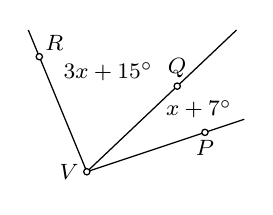
\begin{tikzpicture}
                        % \clip (0,0) rectangle (14.000000,10.000000);
                        {\footnotesize

                        % Marking point V by circle
                        \draw [line width=0.016cm] (3.500000,1.500000) circle (0.040000);%
                        \draw (3.500000,1.500000) node [anchor=east] { $V$ };%

                        % Marking point P by circle
                        \draw [line width=0.016cm] (5.000000,2.000000) circle (0.040000);%
                        \draw (5.000000,2.000000) node [anchor=north] { $P$ };%

                        % Drawing line V P
                        % \draw [line width=0.016cm] (2.600000,1.200000) -- (3.462053,1.487351);%
                        \draw [line width=0.016cm] (3.537947,1.512649) -- (4.962053,1.987351);%
                        \draw [line width=0.016cm] (5.037947,2.012649) -- (5.500000,2.166667);%

                        % Marking point Q by circle
                        \draw [line width=0.016cm] (4.648153,2.587081) circle (0.040000);%
                        \draw (4.648153,2.587081) node [anchor=south] { $Q$ };%

                        % Marking point R by circle
                        \draw [line width=0.016cm] (2.896583,2.961468) circle (0.040000);%
                        \draw (2.866583,2.931468) node [anchor=south west] { $R$ };%

                        % Drawing line V R
                        % \draw [line width=0.016cm] (3.623865,1.200000) -- (3.515265,1.463027);%
                        \draw [line width=0.016cm] (3.484735,1.536973) -- (2.911849,2.924495);%
                        \draw [line width=0.016cm] (2.881318,2.998440) -- (2.756809,3.300000);%

                        % Drawing line V Q
                        % \draw [line width=0.016cm] (3.183146,1.200000) -- (3.470954,1.472499);%
                        \draw [line width=0.016cm] (3.529046,1.527501) -- (4.619106,2.559580);%
                        \draw [line width=0.016cm] (4.677199,2.614582) -- (5.401122,3.300000);%

                        % Marking point {x+7^\circ}
                        \draw (4.924076,2.293541) node  { ${x+7^\circ}$ };%

                        % Marking point {3x+15^\circ}
                        \draw (3.772368,2.774275) node  { ${3x+15^\circ}$ };%
                        }
                    \end{tikzpicture}

                \end{figure}
            \end{exampleblock}}


            \only<3->{\begin{exampleblock}{Naloga}
                Izračunajte velikost kota $\angle SVR$, če je $\angle QVS=50^\circ$.

                \begin{figure}
                    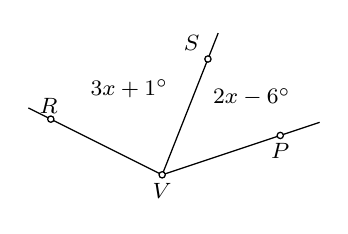
\begin{tikzpicture}
                        % \clip (0,0) rectangle (14.000000,10.000000);
                        {\footnotesize

                        % Marking point V by circle
                        \draw [line width=0.016cm] (3.500000,1.500000) circle (0.040000);%
                        \draw (3.500000,1.500000) node [anchor=north] { $V$ };%

                        % Marking point P by circle
                        \draw [line width=0.016cm] (5.000000,2.000000) circle (0.040000);%
                        \draw (5.000000,2.000000) node [anchor=north] { $P$ };%

                        % Drawing line V P
                        % \draw [line width=0.016cm] (2.600000,1.200000) -- (3.462053,1.487351);%
                        \draw [line width=0.016cm] (3.537947,1.512649) -- (4.962053,1.987351);%
                        \draw [line width=0.016cm] (5.037947,2.012649) -- (5.500000,2.166667);%

                        % Marking point S by circle
                        \draw [line width=0.016cm] (4.081159,2.970460) circle (0.040000);%
                        \draw (4.081159,2.970460) node [anchor=south east] { $S$ };%

                        % Marking point R by circle
                        \draw [line width=0.016cm] (2.085787,2.207107) circle (0.040000);%
                        \draw (2.055787,2.177107) node [anchor=south] { $R$ };%

                        % Drawing line V R
                        % \draw [line width=0.016cm] (4.100000,1.200000) -- (3.535777,1.482111);%
                        \draw [line width=0.016cm] (3.464223,1.517889) -- (2.121564,2.189218);%
                        \draw [line width=0.016cm] (2.050009,2.224995) -- (1.800000,2.350000);%

                        % Drawing line V S
                        % \draw [line width=0.016cm] (3.381433,1.200000) -- (3.485298,1.462800);%
                        \draw [line width=0.016cm] (3.514702,1.537200) -- (4.066457,2.933260);%
                        \draw [line width=0.016cm] (4.095862,3.007660) -- (4.211401,3.300000);%

                        % Marking point {2x-6^\circ}
                        \draw (4.640580,2.485230) node  { ${2x-6^\circ}$ };%

                        % Marking point {3x+1^\circ}
                        \draw (3.083473,2.588784) node  { ${3x+1^\circ}$ };%
                        }
                    \end{tikzpicture}

                \end{figure}
            \end{exampleblock}}

        \end{frame}

                
        \begin{frame}

            \only<2->{\begin{exampleblock}{Naloga}
                Kot $\varphi=76^\circ 36'53''$ zapišite v stopinjah na štiri mesta natančno, 
                kot $\psi=34.78^\circ$ pa zapišite v stopinjah, minutah in sekundah.
            \end{exampleblock}}

            \only<3->{\begin{exampleblock}{Naloga}
                Kotu $\varphi=37^\circ 16'43''$ izračunajte suplementarni in komplementarni kot.
            \end{exampleblock}}

            \only<4->{\begin{exampleblock}{Naloga}
                Razika dveh komplementarnih kotov je $37^\circ 16'$. Izračunajte velikosti kotov.
            \end{exampleblock}}

            \only<5->{\begin{exampleblock}{Naloga}
                Kot $\varphi$ je petkratnik svojega komplementarnega kota. Izračunajte njegovo velikost.
            \end{exampleblock}}

        \end{frame}


        \begin{frame}
            \only<2->{\begin{exampleblock}{Naloga}
                Za vsako od spodnjih izjav ugotovite, ali je pravilna ali nepravilna.
                \begin{itemize}
                    \item Sokota sta suplementarna.
                    % \item Kota z vzporednimi kraki sta skladna.
                    \item Kot z velikostjo $45^\circ$ je komplementaren samemu sebi.
                    \item Dve premici, ki se sekata, lahko določata kota z velikostjo $43^\circ$ in $137^\circ$.
                    \item Vsota velikosti dveh komplementarnih kotov je pravi kot.
                    \item Suplementarna kota sta  vedno tudi sokota.
                \end{itemize}
            \end{exampleblock}}

            \only<3->{\begin{exampleblock}{Naloga}
                Poltrak $VD$ razpolavlja $\angle CVE$, $\angle BVC$ je pravi kot.
                Določite velikosti kotov $\angle AVD$ in $\angle BVE$.

                \begin{figure}
                    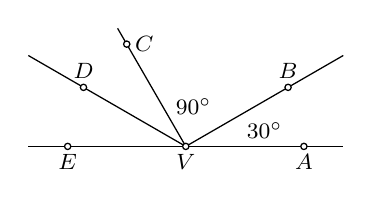
\begin{tikzpicture}
                        % \clip (0,0) rectangle (14.000000,10.000000);
                        {\footnotesize

                        % Marking point V by circle
                        \draw [line width=0.016cm] (4.000000,1.500000) circle (0.040000);%
                        \draw (4.000000,1.500000) node [anchor=north] { $V$ };%

                        % Marking point A by circle
                        \draw [line width=0.016cm] (5.500000,1.500000) circle (0.040000);%
                        \draw (5.500000,1.500000) node [anchor=north] { $A$ };%

                        % Marking point E by circle
                        \draw [line width=0.016cm] (2.500000,1.500000) circle (0.040000);%
                        \draw (2.500000,1.500000) node [anchor=north] { $E$ };%

                        % Drawing line A E
                        \draw [line width=0.016cm] (2.000000,1.500000) -- (2.460000,1.500000);%
                        \draw [line width=0.016cm] (2.540000,1.500000) -- (3.960000,1.500000);%
                        \draw [line width=0.016cm] (4.040000,1.500000) -- (5.460000,1.500000);%
                        \draw [line width=0.016cm] (5.540000,1.500000) -- (6.000000,1.500000);%

                        % Marking point B by circle
                        \draw [line width=0.016cm] (5.299038,2.250000) circle (0.040000);%
                        \draw (5.299038,2.250000) node [anchor=south] { $B$ };%

                        % Marking point C by circle
                        \draw [line width=0.016cm] (3.250000,2.799038) circle (0.040000);%
                        \draw (3.250000,2.799038) node [anchor=west] { $C$ };%

                        % Marking point D by circle
                        \draw [line width=0.016cm] (2.700962,2.250000) circle (0.040000);%
                        \draw (2.700962,2.250000) node [anchor=south] { $D$ };%

                        % Drawing line V D
                        % \draw [line width=0.016cm] (4.519615,1.200000) -- (4.034641,1.480000);%
                        \draw [line width=0.016cm] (3.965359,1.520000) -- (2.735603,2.230000);%
                        \draw [line width=0.016cm] (2.666321,2.270000) -- (2.000000,2.654701);%

                        % Drawing line V C
                        % \draw [line width=0.016cm] (4.173205,1.200000) -- (4.020000,1.465359);%
                        \draw [line width=0.016cm] (3.980000,1.534641) -- (3.270000,2.764397);%
                        \draw [line width=0.016cm] (3.230000,2.833679) -- (3.133975,3.000000);%

                        % Drawing line V B
                        % \draw [line width=0.016cm] (3.480385,1.200000) -- (3.965359,1.480000);%
                        \draw [line width=0.016cm] (4.034641,1.520000) -- (5.264397,2.230000);%
                        \draw [line width=0.016cm] (5.333679,2.270000) -- (6.000000,2.654700);%

                        % Marking point {30^\circ}
                        \draw (5.000000,1.500000) node [anchor=south] { ${30^\circ}$ };%

                        % Marking point {90^\circ}
                        \draw (4.100000,1.800000) node [anchor=south] { ${90^\circ}$ };%
                        }
                    \end{tikzpicture}

                \end{figure}
            \end{exampleblock}}
        \end{frame}





%%%%%%%%%%%%%%%%%%%%%%%%%%%%%%%%%%

    \subsection{Vzporednost in pravokotnost}

        \begin{frame}
            \frametitle{Vzporednost}
            
            \begin{alertblock}{Aksiom o vzporednici}
                Skozi izbrano točko, ki ne leži na premici, lahko tej premici narišemo natanko eno vzporednico.

                \begin{figure}[H]
                    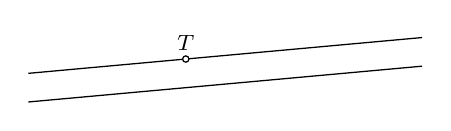
\begin{tikzpicture}
                    % \clip (0,0) rectangle (14.000000,10.000000);
                    {\footnotesize

                    % Drawing line p
                    \draw [line width=0.016cm] (1.000000,1.454545) -- (6.000000,1.909091);%

                    % Drawing line q
                    \draw [line width=0.016cm] (1.000000,1.818182) -- (2.960164,1.996379);%
                    \draw [line width=0.016cm] (3.039836,2.003621) -- (6.000000,2.272727);%

                    % Marking point T by circle
                    \draw [line width=0.016cm] (3.000000,2.000000) circle (0.040000);%
                    \draw (3.000000,2.000000) node [anchor=south] { $T$ };%
                    }
                    \end{tikzpicture}

                \end{figure}

            \end{alertblock}

            \begin{block}{}
                \textbf{Vzporednost} je v množici premic na ravnini \textit{ekvivalenčna relacija}, saj je:
                \begin{itemize}
                    \item \textit{refleksivna}: $p\parallel p$ -- vsaka premica je vzporedna sama sebi;
                    \item \textit{simetrična}: $p\parallel q \Rightarrow q\parallel p$ -- če je premica $p$ vzporedna premici $q$, je tudi premica $q$ vzporedna premici $p$;
                    \item \textit{tranzitivna}: $p\parallel q \land q \parallel r \rightarrow p \parallel r$ -- če je premica $p$ vzporedna premici $q$, premica $q$ pa vzporedna premici $r$, 
                        je tudi premica $p$ vzporedna premici $r$.
                \end{itemize}
            \end{block}

        \end{frame}

        
        \begin{frame}
            \begin{block}{}
                Če vzporednici sekamo s premico, dobimo dve presečišči, ob njiju pa pare \textbf{kotov z vzporednimi kraki}:
                
                \begin{figure}[H]
                    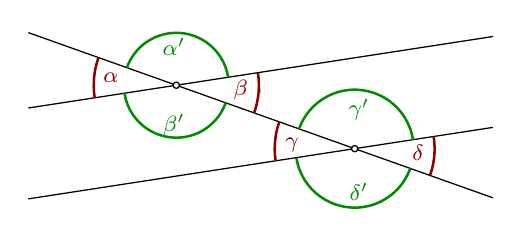
\begin{tikzpicture}
                    % \clip (0,0) rectangle (14.000000,10.000000);
                    {\footnotesize

                    % Drawing line p
                    \draw [line width=0.016cm] (1.300000,1.315385) -- (5.405096,1.946938);%
                    \draw [line width=0.016cm] (5.484166,1.959102) -- (7.200000,2.223077);%

                    % Drawing line q
                    \draw [line width=0.016cm] (1.300000,2.469231) -- (3.139995,2.752307);%
                    \draw [line width=0.016cm] (3.219065,2.764472) -- (7.200000,3.376923);%

                    % Drawing line r
                    \draw [line width=0.016cm] (1.300000,3.426667) -- (3.141842,2.771790);%
                    \draw [line width=0.016cm] (3.217219,2.744989) -- (5.406942,1.966421);%
                    \draw [line width=0.016cm] (5.482319,1.939620) -- (7.200000,1.328889);%

                    % Marking point U by circle
                    \draw [line width=0.016cm] (5.444631,1.953020) circle (0.040000);%

                    % Marking point V by circle
                    \draw [line width=0.016cm] (3.179530,2.758389) circle (0.040000);%

                    % Changing color 139 0 0
                    \definecolor{r139g0b0}{rgb}{0.545098,0.000000,0.000000}%
                    \color{r139g0b0}% 

                    % Drawing arc V L 28.32
                    \draw [line width=0.032cm] (2.191446,3.109708) -- (2.187982,3.099807) arc (161:188:1.048682 and 1.048682) -- (2.143042,2.598930);%

                    % Drawing arc V M 28.32
                    \draw [line width=0.032cm] (4.167614,2.407070) -- (4.171079,2.416971) arc (341:360:1.048682 and 1.048682) --(4.228212,2.758389) arc (0:8:1.048682 and 1.048682) -- (4.216018,2.917849);%

                    % Drawing arc U N 28.32
                    \draw [line width=0.032cm] (4.487996,2.293157) -- (4.484642,2.283571) arc (161:188:1.015305 and 1.015305) -- (4.441133,1.798636);%

                    % Drawing arc U O 28.32
                    \draw [line width=0.032cm] (6.401266,1.612883) -- (6.404620,1.622469) arc (341:360:1.015305 and 1.015305) --(6.459935,1.953020) arc (0:8:1.015305 and 1.015305) -- (6.448129,2.107404);%

                    % Marking point \alpha
                    \draw (2.350000,2.850000) node  { $\alpha$ };%

                    % Marking point \beta
                    \draw (4.000000,2.700000) node  { $\beta$ };%

                    % Marking point \gamma
                    \draw (4.650000,2.000000) node  { $\gamma$ };%

                    % Marking point \delta
                    \draw (6.250000,1.900000) node  { $\delta$ };%

                    % Changing color 0 139 0
                    \definecolor{r0g139b0}{rgb}{0.000000,0.545098,0.000000}%
                    \color{r0g139b0}% 

                    % Drawing arc V J 151.68
                    \draw [line width=0.032cm] (3.837639,2.859637) -- (3.837184,2.862551) arc (9:160:0.665852 and 0.665852) -- (2.552155,2.981456);%

                    % Drawing arc V K 151.68
                    \draw [line width=0.032cm] (2.521421,2.657142) -- (2.521876,2.654227) arc (189:340:0.665852 and 0.665852) -- (3.806905,2.535322);%

                    % Drawing arc U P 151.68
                    \draw [line width=0.032cm] (6.184950,2.066915) -- (6.184438,2.070194) arc (9:160:0.749029 and 0.749029) -- (4.738885,2.203952);%

                    % Drawing arc U R 151.68
                    \draw [line width=0.032cm] (4.704312,1.839125) -- (4.704824,1.835846) arc (189:340:0.749029 and 0.749029) -- (6.150377,1.702088);%

                    % Marking point \alpha'
                    \draw (3.150000,3.250000) node  { $\alpha'$ };%

                    % Marking point \beta'
                    \draw (3.150000,2.250000) node  { $\beta'$ };%

                    % Marking point \gamma'
                    \draw (5.500000,2.450000) node  { $\gamma'$ };%

                    % Marking point \delta'
                    \draw (5.500000,1.400000) node  { $\delta'$ };%
                    \color{black}
                    }
                    \end{tikzpicture}
                    
                \end{figure}

                \begin{itemize}
                    \item pari kotov $(\alpha, \gamma)$, $(\beta, \delta)$, $(\alpha', \gamma')$, $(\beta', \delta')$ imajo oba kraka vzporedna v isto smer;
                    \item pari kotov z istim vrhom $(\alpha, \beta)$; $(\gamma, \delta)$, $(\alpha', \beta')$; $(\gamma', \delta')$ imajo oba kraka vzporedna v nasprotno smer -- \textbf{sovršni koti};
                    \item pari kotov $(\alpha, \alpha')$, $(\beta, \beta')$, $(\gamma,\gamma')$, $(\delta,\delta')$ imajo en krak vzporeden v isto smer, drugi krak pa vzporeden v nasprotno smer.
                \end{itemize}
            \end{block}
        \end{frame}


        \begin{frame}
            \begin{alertblock}{Izrek}
                Para konveksnih kotov z vzporednimi kraki sta ali skladna ali suplementarna.

                \begin{figure}[H]
                    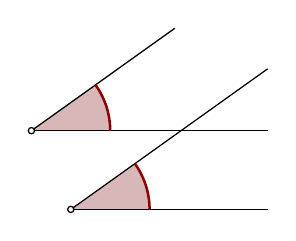
\begin{tikzpicture}
                    % \clip (0,0) rectangle (14.000000,10.000000);
                    {\footnotesize

                    % Changing color 215 183 183
                    \definecolor{r215g183b183}{rgb}{0.843137,0.717647,0.717647}%
                    \color{r215g183b183}% 

                    % Filling circle arc V D 35.54
                    \fill (1.500000,2.500000) -- (2.500000,2.500000) arc (0:35:1.000000 and 1.000000) -- (2.313733,3.081238) -- cycle;%

                    % Filling circle arc U E 35.54
                    \fill (2.000000,1.500000) -- (3.000000,1.500000) arc (0:35:1.000000 and 1.000000) -- (2.813733,2.081238) -- cycle;%

                    % Changing color 0 0 0
                    \definecolor{r0g0b0}{rgb}{0.000000,0.000000,0.000000}%
                    \color{r0g0b0}% 

                    % Marking point V by circle
                    \draw [line width=0.016cm] (1.500000,2.500000) circle (0.040000);%

                    % Drawing line V A
                    % \draw [line width=0.016cm] (1.000000,2.500000) -- (1.460000,2.500000);%
                    \draw [line width=0.016cm] (1.540000,2.500000) -- (4.500000,2.500000);%

                    % Drawing line V B
                    \draw [line width=0.016cm] (3.320000,3.800000) -- (1.532549,2.523250);%
                    % \draw [line width=0.016cm] (1.467451,2.476750) -- (1.000000,2.142857);%

                    % Marking point U by circle
                    \draw [line width=0.016cm] (2.000000,1.500000) circle (0.040000);%

                    % Drawing line r
                    % \draw [line width=0.016cm] (1.300000,1.000000) -- (1.967451,1.476750);%
                    \draw [line width=0.016cm] (2.032549,1.523250) -- (4.500000,3.285714);%

                    % Drawing line s
                    % \draw [line width=0.016cm] (1.000000,1.500000) -- (1.960000,1.500000);%
                    \draw [line width=0.016cm] (2.040000,1.500000) -- (4.500000,1.500000);%

                    % Changing color 139 0 0
                    \definecolor{r139g0b0}{rgb}{0.545098,0.000000,0.000000}%
                    \color{r139g0b0}% 

                    % Drawing arc V D 35.54
                    \draw [line width=0.032cm] (2.500000,2.500000) arc (360:360:1.000000 and 1.000000) --(2.500000,2.500000) arc (0:35:1.000000 and 1.000000) -- (2.313733,3.081238);%

                    % Drawing arc U E 35.54
                    \draw [line width=0.032cm] (3.000000,1.500000) arc (360:360:1.000000 and 1.000000) --(3.000000,1.500000) arc (0:35:1.000000 and 1.000000) -- (2.813733,2.081238);%
                    \color{black}
                    }
                    \end{tikzpicture} ~~~~
                    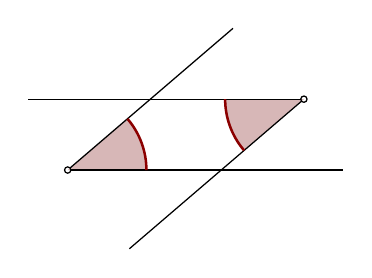
\begin{tikzpicture}
                    % \clip (0,0) rectangle (14.000000,10.000000);
                    {\footnotesize

                    % Changing color 215 183 183
                    \definecolor{r215g183b183}{rgb}{0.843137,0.717647,0.717647}%
                    \color{r215g183b183}% 

                    % Filling circle arc V D 40.60
                    \fill (1.500000,2.000000) -- (2.500000,2.000000) arc (0:40:1.000000 and 1.000000) -- (2.259257,2.650791) -- cycle;%

                    % Filling circle arc U E 40.60
                    \fill (4.500000,2.900000) -- (3.500000,2.900000) arc (180:220:1.000000 and 1.000000) -- (3.740743,2.249209) -- cycle;%

                    % Changing color 0 0 0
                    \definecolor{r0g0b0}{rgb}{0.000000,0.000000,0.000000}%
                    \color{r0g0b0}% 

                    % Marking point V by circle
                    \draw [line width=0.016cm] (1.500000,2.000000) circle (0.040000);%

                    % Drawing line V A
                    % \draw [line width=0.016cm] (1.000000,2.000000) -- (1.460000,2.000000);%
                    \draw [line width=0.016cm] (1.540000,2.000000) -- (5.000000,2.000000);%

                    % Drawing line V B
                    \draw [line width=0.016cm] (3.600000,3.800000) -- (1.530370,2.026032);%
                    % \draw [line width=0.016cm] (1.469630,1.973968) -- (1.000000,1.571429);%

                    % Marking point U by circle
                    \draw [line width=0.016cm] (4.500000,2.900000) circle (0.040000);%

                    % Drawing line r
                    \draw [line width=0.016cm] (2.283333,1.000000) -- (4.469630,2.873968);%
                    % \draw [line width=0.016cm] (4.530370,2.926032) -- (5.000000,3.328571);%

                    % Drawing line s
                    \draw [line width=0.016cm] (1.000000,2.900000) -- (4.460000,2.900000);%
                    % \draw [line width=0.016cm] (4.540000,2.900000) -- (5.000000,2.900000);%

                    % Changing color 139 0 0
                    \definecolor{r139g0b0}{rgb}{0.545098,0.000000,0.000000}%
                    \color{r139g0b0}% 

                    % Drawing arc V D 40.60
                    \draw [line width=0.032cm] (2.500000,2.000000) arc (360:360:1.000000 and 1.000000) --(2.500000,2.000000) arc (0:40:1.000000 and 1.000000) -- (2.259257,2.650791);%

                    % Drawing arc U E 40.60
                    \draw [line width=0.032cm] (3.500000,2.900000) arc (180:220:1.000000 and 1.000000) -- (3.740743,2.249209);%
                    \color{black}
                    }
                    \end{tikzpicture} ~~~~
                    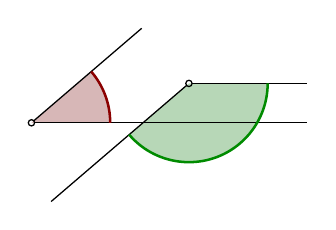
\begin{tikzpicture}
                    % \clip (0,0) rectangle (14.000000,10.000000);
                    {\footnotesize

                    % Changing color 215 183 183
                    \definecolor{r215g183b183}{rgb}{0.843137,0.717647,0.717647}%
                    \color{r215g183b183}% 

                    % Filling circle arc V D 40.60
                    \fill (1.500000,2.000000) -- (2.500000,2.000000) arc (0:40:1.000000 and 1.000000) -- (2.259257,2.650791) -- cycle;%

                    % Changing color 183 215 183
                    \definecolor{r183g215b183}{rgb}{0.717647,0.843137,0.717647}%
                    \color{r183g215b183}% 

                    % Filling circle arc U G 139.40
                    \fill (3.500000,2.500000) -- (2.740743,1.849209) -- (2.745290,1.843941) arc (221:360:1.000000 and 1.000000) --(4.500000,2.500000) arc (0:0:1.000000 and 1.000000) -- cycle;%

                    % Changing color 0 0 0
                    \definecolor{r0g0b0}{rgb}{0.000000,0.000000,0.000000}%
                    \color{r0g0b0}% 

                    % Marking point V by circle
                    \draw [line width=0.016cm] (1.500000,2.000000) circle (0.040000);%

                    % Drawing line V A
                    % \draw [line width=0.016cm] (1.000000,2.000000) -- (1.460000,2.000000);%
                    \draw [line width=0.016cm] (1.540000,2.000000) -- (5.000000,2.000000);%

                    % Drawing line V B
                    \draw [line width=0.016cm] (2.900000,3.200000) -- (1.530370,2.026032);%
                    % \draw [line width=0.016cm] (1.469630,1.973968) -- (1.000000,1.571429);%

                    % Marking point U by circle
                    \draw [line width=0.016cm] (3.500000,2.500000) circle (0.040000);%

                    % Drawing line r
                    \draw [line width=0.016cm] (1.750000,1.000000) -- (3.469630,2.473968);%
                    % \draw [line width=0.016cm] (3.530370,2.526032) -- (4.316667,3.200000);%

                    % Drawing line s
                    % \draw [line width=0.016cm] (1.000000,2.500000) -- (3.460000,2.500000);%
                    \draw [line width=0.016cm] (3.540000,2.500000) -- (5.000000,2.500000);%

                    % Changing color 139 0 0
                    \definecolor{r139g0b0}{rgb}{0.545098,0.000000,0.000000}%
                    \color{r139g0b0}% 

                    % Drawing arc V D 40.60
                    \draw [line width=0.032cm] (2.500000,2.000000) arc (360:360:1.000000 and 1.000000) --(2.500000,2.000000) arc (0:40:1.000000 and 1.000000) -- (2.259257,2.650791);%

                    % Changing color 0 139 0
                    \definecolor{r0g139b0}{rgb}{0.000000,0.545098,0.000000}%
                    \color{r0g139b0}% 

                    % Drawing arc U G 139.40
                    \draw [line width=0.032cm] (2.740743,1.849209) -- (2.745290,1.843941) arc (221:360:1.000000 and 1.000000);%
                    \color{black}
                    }
                    \end{tikzpicture}

                \end{figure}
            \end{alertblock}

            \begin{block}{}
                Sovršna kota sta skladna -- imata isti sokot.

                \begin{figure}[H]
                    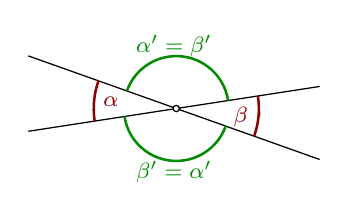
\begin{tikzpicture}
                    % \clip (0,0) rectangle (14.000000,10.000000);
                    {\footnotesize

                    % Drawing line p

                    % Drawing line q
                    \draw [line width=0.016cm] (1.300000,2.469231) -- (3.139995,2.752307);%
                    \draw [line width=0.016cm] (3.219065,2.764472) -- (5.000000,3.038462);%

                    % Drawing line r
                    \draw [line width=0.016cm] (1.300000,3.426667) -- (3.141842,2.771790);%
                    \draw [line width=0.016cm] (3.217219,2.744989) -- (5.000000,2.111111);%

                    % Marking point U by circle

                    % Marking point V by circle
                    \draw [line width=0.016cm] (3.179530,2.758389) circle (0.040000);%

                    % Changing color 139 0 0
                    \definecolor{r139g0b0}{rgb}{0.545098,0.000000,0.000000}%
                    \color{r139g0b0}% 

                    % Drawing arc V L 28.32
                    \draw [line width=0.032cm] (2.191446,3.109708) -- (2.187982,3.099807) arc (161:188:1.048682 and 1.048682) -- (2.143042,2.598930);%

                    % Drawing arc V M 28.32
                    \draw [line width=0.032cm] (4.167614,2.407070) -- (4.171079,2.416971) arc (341:360:1.048682 and 1.048682) --(4.228212,2.758389) arc (0:8:1.048682 and 1.048682) -- (4.216018,2.917849);%

                    % Marking point \alpha
                    \draw (2.350000,2.850000) node  { $\alpha$ };%

                    % Marking point \beta
                    \draw (4.000000,2.650000) node  { $\beta$ };%

                    % Changing color 0 139 0
                    \definecolor{r0g139b0}{rgb}{0.000000,0.545098,0.000000}%
                    \color{r0g139b0}% 

                    % Drawing arc V J 151.68
                    \draw [line width=0.032cm] (3.837639,2.859637) -- (3.837184,2.862551) arc (9:160:0.665852 and 0.665852) -- (2.552155,2.981456);%

                    % Drawing arc V K 151.68
                    \draw [line width=0.032cm] (2.521421,2.657142) -- (2.521876,2.654227) arc (189:340:0.665852 and 0.665852) -- (3.806905,2.535322);%

                    % Marking point \alpha'
                    \draw (3.150000,3.55000) node  { $\alpha'=\beta'$ };%

                    % Marking point \beta'
                    \draw (3.150000,1.95000) node  { $\beta'=\alpha'$ };%
                    \color{black}
                    }
                    \end{tikzpicture}
                \end{figure}
            \end{block}
        \end{frame}




        \begin{frame}
            \frametitle{Preslikave na ravnini}

            \large\textbf{Pravokotna projekcija}
            ~\\

            \normalsize
            \begin{columns}
                \column{0.62\textwidth}
                    \begin{alertblock}{}
                        Dani sta točka $T$ in premica $p$. Naj bo $q$ tista pravokotnica na premico $p$, ki poteka skozi točko $T$. 
                        Presečišče $T'$ premice $q$ s premico $p$ imenujemo \textbf{pravokotna projekcija} točke $T$ na premico $p$. 
                        Točka $T'$ je točki $T$ najbližja točka premice $p$. \\
                    \end{alertblock}
                    % ~\\
                    \begin{alertblock}{}
                        \textbf{Razdalja} točke $T$ od premice $p$ je: \\ $\quad \quad \quad \quad d(T,p)=d(T,T')=\left\lvert TT'\right\rvert$. \\
                    \end{alertblock} ~\\

                \column{0.35\textwidth}            
                    % \begin{figure}
                    % 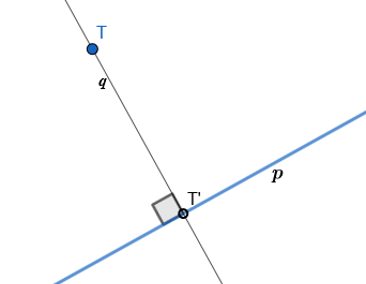
\includegraphics[scale=0.5]{Slike in skice/Pravokotna_projekcija.png}
                    % \end{figure}

                    \begin{figure}
                        \begin{tikzpicture}
                            % \clip (0,0) rectangle (14.000000,10.000000);
                            {\footnotesize
                            
                            % Drawing line Q
                            \draw [line width=0.016cm] (3.000000,1.000000) -- (2.932918,1.134164);%
                            \draw [line width=0.016cm] (2.899377,1.201246) -- (2.832295,1.335410);%
                            \draw [line width=0.016cm] (2.798754,1.402492) -- (2.731672,1.536656);%
                            \draw [line width=0.016cm] (2.698131,1.603738) -- (2.631049,1.737902);%
                            \draw [line width=0.016cm] (2.582111,1.835777) -- (2.530426,1.939149);%
                            \draw [line width=0.016cm] (2.496885,2.006231) -- (2.429803,2.140395);%
                            \draw [line width=0.016cm] (2.396262,2.207477) -- (2.329180,2.341641);%
                            \draw [line width=0.016cm] (2.295639,2.408723) -- (2.228557,2.542887);%
                            \draw [line width=0.016cm] (2.195016,2.609969) -- (2.127933,2.744133);%
                            \draw [line width=0.016cm] (2.094392,2.811215) -- (2.027310,2.945379);%
                            \draw [line width=0.016cm] (1.993769,3.012461) -- (1.926687,3.146625);%
                            \draw [line width=0.016cm] (1.893146,3.213707) -- (1.826064,3.347871);%
                            \draw [line width=0.016cm] (1.792523,3.414953) -- (1.725441,3.549117);%
                            \draw [line width=0.016cm] (1.691900,3.616200) -- (1.624818,3.750364);%
                            \draw [line width=0.016cm] (1.591277,3.817446) -- (1.524195,3.951610);%
                            \draw [line width=0.016cm] (1.482111,4.035777) -- (1.423572,4.152856);%
                            \draw [line width=0.016cm] (1.390031,4.219938) -- (1.322949,4.354102);%
                            \draw [line width=0.016cm] (1.289408,4.421184) -- (1.250000,4.500000);%
                            
                            % Marking point q
                            \draw (1.847000,3.306000) node [anchor=east] { $q$ };%
                            
                            % Marking point T by circle
                            \draw [line width=0.016cm] (1.500000,4.000000) circle (0.040000);%
                            \draw (1.550000,4.000000) node [anchor=south] { $T$ };%
                            
                            % Marking point \frac{\pi}{2}
                            \draw (2.250000,2.000000) node  { $\frac{\pi}{2}$ };%
                            
                            % Changing color 0 0 255
                            \definecolor{r0g0b255}{rgb}{0.000000,0.000000,1.000000}%
                            \color{r0g0b255}% 
                            
                            % Drawing line P
                            \draw [line width=0.016cm] (1.000000,1.000000) -- (2.564223,1.782111);%
                            \draw [line width=0.016cm] (2.635777,1.817889) -- (4.500000,2.750000);%
                            
                            % Marking point p
                            \draw (4.155000,2.578000) node [anchor=north] { $p$ };%
                            
                            % Changing color 255 0 0
                            \definecolor{r255g0b0}{rgb}{1.000000,0.000000,0.000000}%
                            \color{r255g0b0}% 
                            
                            % Marking point T' by circle
                            \draw [line width=0.016cm] (2.600000,1.800000) circle (0.040000);%
                            \draw (2.500000,1.900000) node [anchor=south west] { $T'$ };%
                            \color{black}
                            }
                        \end{tikzpicture}
                    \end{figure}
            \end{columns}

            Pravokotna projekcija daljice $AB$ na premico je daljica $A'B'$, katere krajišči sta pravokotni projekciji točk $A$ in $B$.


            \note{
                TABLA: konstrukcija pravokotne projekcije točke  z ravnilom in šestilom
                \\
                TABLA: konstruckija pravokotne projekcije daljice z ravnilom in šestilom
            }


        \end{frame}

        \begin{frame}
            \large\textbf{Toge preslikave}
            ~\\
            \normalsize

            \begin{alertblock}{}
                \textbf{Toga preslikava} (izometrija) je preslikava v ravnini, ki ohranja razdalje.
                \begin{align*}
                    \tau:~ &A \mapsto A' \\ 
                    \tau:~ &B \mapsto B' \\ 
                    d(A,B)&=d(A',B')
                \end{align*}
            \end{alertblock}

            Med toge preslikave spadajo:
                \begin{itemize}
                    \item \textbf{vzporedni premiki};
                    \item \textbf{zrcaljenje preko premice};
                    \item \textbf{zrcaljenje preko točke};
                    \item \textbf{rotacija okoli točke}.
                \end{itemize}

            Če kombiniramo več togih preslikav, je dobljena preslikava spet toga preslikava.


            \note{
                Tudi poimenovanje skladnostna preslikava.
                
            }

        \end{frame}

        \begin{frame}
            \large\textbf{Vzporedni premik/translacija}
            ~\\

            \normalsize
            \textbf{Vzporedni premik} ali \textbf{translacija} za dano usmerjeno daljico $\overrightarrow{MN}$ preslika točko $T$ v tako točko $T'$, da sta daljici $TT'$ in $MN$ enako dolgi, vzporedni in enako usmerjeni. \\  %(vektorja $\overrightarrow{TT'}$ in $\overrightarrow{AB}$ sta enaka). \\
            
            % \begin{figure}
            %     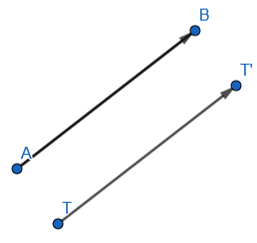
\includegraphics[scale=0.5]{Slike in skice/Vzporedni_premik_tocke.png}
            %     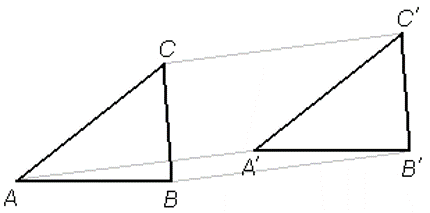
\includegraphics[scale=0.5]{Slike in skice/Vzporedni_premik_trikotnika.png}
            % \end{figure}

            \begin{figure}
                \begin{tikzpicture}
                    % \clip (0,0) rectangle (14.000000,10.000000);
                    {\footnotesize
                    
                    % Drawing segment M N
                    \draw [line width=0.016cm] (1.537947,2.512649) -- (4.462053,3.487351);%
                    
                    % Drawing arrow M N 1.00
                    \draw [line width=0.016cm] (4.205447,3.443092) -- (4.460726,3.492412);%
                    \draw [line width=0.016cm] (4.205447,3.443092) -- (4.405943,3.468648);%
                    \draw [line width=0.016cm] (4.230213,3.368795) -- (4.464028,3.482506);%
                    \draw [line width=0.016cm] (4.230213,3.368795) -- (4.405943,3.468648);%
                    
                    % Drawing segment T T'
                    \draw [line width=0.016cm] (2.037947,1.512649) -- (2.142302,1.547434);%
                    \draw [line width=0.016cm] (2.213454,1.571151) -- (2.355756,1.618585);%
                    \draw [line width=0.016cm] (2.426907,1.642302) -- (2.569210,1.689737);%
                    \draw [line width=0.016cm] (2.640361,1.713454) -- (2.782664,1.760888);%
                    \draw [line width=0.016cm] (2.853815,1.784605) -- (2.996117,1.832039);%
                    \draw [line width=0.016cm] (3.067269,1.855756) -- (3.209571,1.903190);%
                    \draw [line width=0.016cm] (3.280722,1.926907) -- (3.423025,1.974342);%
                    \draw [line width=0.016cm] (3.494176,1.998059) -- (3.636479,2.045493);%
                    \draw [line width=0.016cm] (3.707630,2.069210) -- (3.849932,2.116644);%
                    \draw [line width=0.016cm] (3.921084,2.140361) -- (4.063386,2.187795);%
                    \draw [line width=0.016cm] (4.134537,2.211512) -- (4.276840,2.258947);%
                    \draw [line width=0.016cm] (4.347991,2.282664) -- (4.490294,2.330098);%
                    \draw [line width=0.016cm] (4.561445,2.353815) -- (4.703747,2.401249);%
                    \draw [line width=0.016cm] (4.774899,2.424966) -- (4.917201,2.472400);%
                    
                    % Drawing arrow T T' 1.00
                    \draw [line width=0.016cm] (4.705447,2.443092) -- (4.960726,2.492412);%
                    \draw [line width=0.016cm] (4.705447,2.443092) -- (4.905943,2.468648);%
                    \draw [line width=0.016cm] (4.730213,2.368795) -- (4.964028,2.482506);%
                    \draw [line width=0.016cm] (4.730213,2.368795) -- (4.905943,2.468648);%
                    
                    % Marking point T by circle
                    \draw [line width=0.016cm] (2.000000,1.500000) circle (0.040000);%
                    \draw (2.000000,1.500000) node [anchor=north] { $T$ };%
                    
                    % Marking point A by circle
                    \draw [line width=0.016cm] (6.000000,2.000000) circle (0.040000);%
                    \draw (6.000000,2.000000) node [anchor=north] { $A$ };%
                    
                    % Marking point B by circle
                    \draw [line width=0.016cm] (9.000000,2.000000) circle (0.040000);%
                    \draw (9.000000,2.000000) node [anchor=north] { $B$ };%
                    
                    % Marking point C by circle
                    \draw [line width=0.016cm] (7.000000,4.000000) circle (0.040000);%
                    \draw (7.000000,4.000000) node [anchor=south] { $C$ };%
                    
                    % Drawing segment A B
                    \draw [line width=0.016cm] (6.040000,2.000000) -- (8.960000,2.000000);%
                    
                    % Drawing segment B C
                    \draw [line width=0.016cm] (8.971716,2.028284) -- (7.028284,3.971716);%
                    
                    % Drawing segment A C
                    \draw [line width=0.016cm] (6.017889,2.035777) -- (6.982111,3.964223);%
                    
                    % Drawing segment A' B'
                    \draw [line width=0.016cm] (9.040000,3.000000) -- (11.960000,3.000000);%
                    
                    % Drawing segment B' C'
                    \draw [line width=0.016cm] (11.971716,3.028284) -- (10.028284,4.971716);%
                    
                    % Drawing segment A' C'
                    \draw [line width=0.016cm] (9.017889,3.035777) -- (9.982111,4.964223);%
                    
                    % Drawing segment A A'
                    \draw [line width=0.016cm] (6.037947,2.012649) -- (6.142302,2.047434);%
                    \draw [line width=0.016cm] (6.213454,2.071151) -- (6.355756,2.118585);%
                    \draw [line width=0.016cm] (6.426907,2.142302) -- (6.569210,2.189737);%
                    \draw [line width=0.016cm] (6.640361,2.213454) -- (6.782664,2.260888);%
                    \draw [line width=0.016cm] (6.853815,2.284605) -- (6.996117,2.332039);%
                    \draw [line width=0.016cm] (7.067269,2.355756) -- (7.209571,2.403190);%
                    \draw [line width=0.016cm] (7.280722,2.426907) -- (7.423025,2.474342);%
                    \draw [line width=0.016cm] (7.494176,2.498059) -- (7.636479,2.545493);%
                    \draw [line width=0.016cm] (7.707630,2.569210) -- (7.849932,2.616644);%
                    \draw [line width=0.016cm] (7.921084,2.640361) -- (8.063386,2.687795);%
                    \draw [line width=0.016cm] (8.134537,2.711512) -- (8.276840,2.758947);%
                    \draw [line width=0.016cm] (8.347991,2.782664) -- (8.490294,2.830098);%
                    \draw [line width=0.016cm] (8.561445,2.853815) -- (8.703747,2.901249);%
                    \draw [line width=0.016cm] (8.774899,2.924966) -- (8.917201,2.972400);%
                    
                    % Drawing segment B B'
                    \draw [line width=0.016cm] (9.037947,2.012649) -- (9.142302,2.047434);%
                    \draw [line width=0.016cm] (9.213454,2.071151) -- (9.355756,2.118585);%
                    \draw [line width=0.016cm] (9.426907,2.142302) -- (9.569210,2.189737);%
                    \draw [line width=0.016cm] (9.640361,2.213454) -- (9.782664,2.260888);%
                    \draw [line width=0.016cm] (9.853815,2.284605) -- (9.996117,2.332039);%
                    \draw [line width=0.016cm] (10.067269,2.355756) -- (10.209571,2.403190);%
                    \draw [line width=0.016cm] (10.280722,2.426907) -- (10.423025,2.474342);%
                    \draw [line width=0.016cm] (10.494176,2.498059) -- (10.636479,2.545493);%
                    \draw [line width=0.016cm] (10.707630,2.569210) -- (10.849932,2.616644);%
                    \draw [line width=0.016cm] (10.921084,2.640361) -- (11.063386,2.687795);%
                    \draw [line width=0.016cm] (11.134537,2.711512) -- (11.276840,2.758947);%
                    \draw [line width=0.016cm] (11.347991,2.782664) -- (11.490294,2.830098);%
                    \draw [line width=0.016cm] (11.561445,2.853815) -- (11.703747,2.901249);%
                    \draw [line width=0.016cm] (11.774899,2.924966) -- (11.917201,2.972400);%
                    
                    % Drawing segment C C'
                    \draw [line width=0.016cm] (7.037947,4.012649) -- (7.142302,4.047434);%
                    \draw [line width=0.016cm] (7.213454,4.071151) -- (7.355756,4.118585);%
                    \draw [line width=0.016cm] (7.426907,4.142302) -- (7.569210,4.189737);%
                    \draw [line width=0.016cm] (7.640361,4.213454) -- (7.782664,4.260888);%
                    \draw [line width=0.016cm] (7.853815,4.284605) -- (7.996117,4.332039);%
                    \draw [line width=0.016cm] (8.067269,4.355756) -- (8.209571,4.403190);%
                    \draw [line width=0.016cm] (8.280722,4.426907) -- (8.423025,4.474342);%
                    \draw [line width=0.016cm] (8.494176,4.498059) -- (8.636479,4.545493);%
                    \draw [line width=0.016cm] (8.707630,4.569210) -- (8.849932,4.616644);%
                    \draw [line width=0.016cm] (8.921084,4.640361) -- (9.063386,4.687795);%
                    \draw [line width=0.016cm] (9.134537,4.711512) -- (9.276840,4.758947);%
                    \draw [line width=0.016cm] (9.347991,4.782664) -- (9.490294,4.830098);%
                    \draw [line width=0.016cm] (9.561445,4.853815) -- (9.703747,4.901249);%
                    \draw [line width=0.016cm] (9.774899,4.924966) -- (9.917201,4.972400);%
                    
                    % Changing color 0 0 255
                    \definecolor{r0g0b255}{rgb}{0.000000,0.000000,1.000000}%
                    \color{r0g0b255}% 
                    
                    % Marking point M by circle
                    \draw [line width=0.016cm] (1.500000,2.500000) circle (0.040000);%
                    \draw (1.500000,2.500000) node [anchor=north] { $M$ };%
                    
                    % Marking point N by circle
                    \draw [line width=0.016cm] (4.500000,3.500000) circle (0.040000);%
                    \draw (4.500000,3.500000) node [anchor=south] { $N$ };%
                    
                    % Changing color 255 0 0
                    \definecolor{r255g0b0}{rgb}{1.000000,0.000000,0.000000}%
                    \color{r255g0b0}% 
                    
                    % Marking point T' by circle
                    \draw [line width=0.016cm] (5.000000,2.500000) circle (0.040000);%
                    \draw (5.000000,2.500000) node [anchor=south] { $T'$ };%
                    
                    % Marking point C' by circle
                    \draw [line width=0.016cm] (10.000000,5.000000) circle (0.040000);%
                    \draw (10.000000,5.000000) node [anchor=south] { $C'$ };%
                    
                    % Marking point A' by circle
                    \draw [line width=0.016cm] (9.000000,3.000000) circle (0.040000);%
                    \draw (9.000000,3.000000) node [anchor=north] { $A'$ };%
                    
                    % Marking point B' by circle
                    \draw [line width=0.016cm] (12.000000,3.000000) circle (0.040000);%
                    \draw (12.000000,3.000000) node [anchor=north] { $B'$ };%
                    \color{black}
                    }
                \end{tikzpicture}
                    
            \end{figure}

            Vzporedni premik ohranja orientacijo likov, daljice preslika v enako dolge vzporedne daljice, ohranja velikost kotov, like preslika v skladne like, nima negibnih točk za $\overrightarrow{MN}\neq \overrightarrow{0}$.


            \note{
                TABLA: konstrukcija translacije točke in trikotnika
                \\
                S pomočjo skic na tabli/okviru ugotovitev lastnosti translacije.
            }

        \end{frame}



        % \begin{frame}
            
        %     Če smo kot  odmerili v smeri, ki je nasprotna smeri vrtenja urnega kazalca, smo točko $T$ zavrteli v \textbf{pozitivni smeri} za kot $\alpha$, sicer pa v \textbf{negativni smeri}. 
        %     Namesto smeri vrtenja lahko usmerimo kot: vrtenju v pozitivni smeri ustreza \textbf{pozitivni kot}, vrtenju v negativni smeri pa \textbf{negativni kot}. \\
        %     ~\\


        % \end{frame}


        \begin{frame}
            \large\textbf{Zrcaljenje preko premice}
            ~\\
            ~\\
            \normalsize
            \textbf{Zrcaljenje čez premico} $p$ preslika točko $T$ v tako točko $T'$, da premica $p$ pod pravim kotom razpolavlja daljico $TT'$.
            
            % \begin{figure}
            %     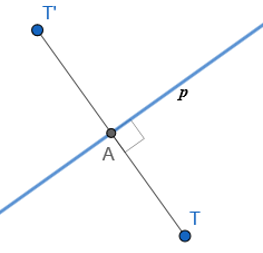
\includegraphics[scale=0.5]{Slike in skice/Zrcaljenje_tocke_cez_premico.png}
            %     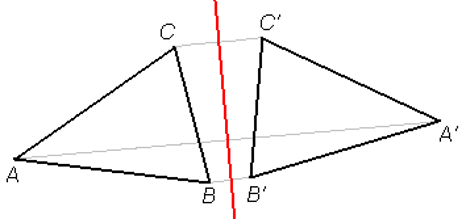
\includegraphics[scale=0.5]{Slike in skice/Zrcaljenje_lika_cez_premico.png}
            % \end{figure}

            \begin{figure}
                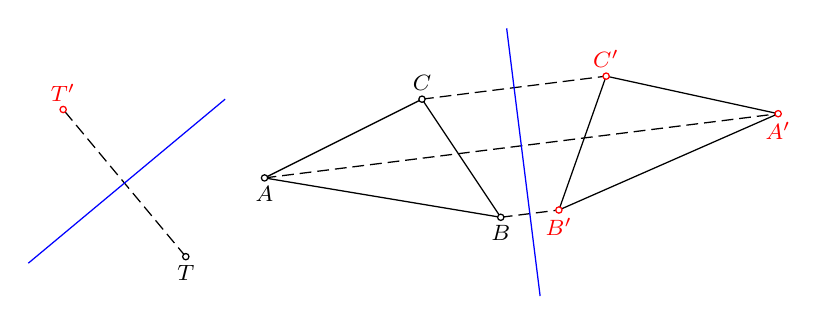
\begin{tikzpicture}
                    % \clip (0,0) rectangle (14.000000,10.000000);
                    {\footnotesize
                    
                    % Marking point T by circle
                    \draw [line width=0.016cm] (3.500000,1.500000) circle (0.040000);%
                    \draw (3.500000,1.500000) node [anchor=north] { $T$ };%
                    
                    % Drawing segment T T'
                    \draw [line width=0.016cm] (3.474393,1.530729) -- (3.403972,1.615233);%
                    \draw [line width=0.016cm] (3.355959,1.672850) -- (3.259931,1.788083);%
                    \draw [line width=0.016cm] (3.211917,1.845700) -- (3.115889,1.960933);%
                    \draw [line width=0.016cm] (3.067876,2.018549) -- (2.971848,2.133783);%
                    \draw [line width=0.016cm] (2.923834,2.191399) -- (2.827806,2.306632);%
                    \draw [line width=0.016cm] (2.779793,2.364249) -- (2.683765,2.479482);%
                    \draw [line width=0.016cm] (2.635751,2.537099) -- (2.539723,2.652332);%
                    \draw [line width=0.016cm] (2.491710,2.709949) -- (2.395682,2.825182);%
                    \draw [line width=0.016cm] (2.347668,2.882798) -- (2.251640,2.998031);%
                    \draw [line width=0.016cm] (2.203627,3.055648) -- (2.107599,3.170881);%
                    \draw [line width=0.016cm] (2.059585,3.228498) -- (1.968230,3.338124);%
                    
                    % Drawing segment C C'
                    \draw [line width=0.016cm] (6.539691,3.504961) -- (6.648842,3.518605);%
                    \draw [line width=0.016cm] (6.723263,3.527908) -- (6.872104,3.546513);%
                    \draw [line width=0.016cm] (6.946525,3.555816) -- (7.095367,3.574421);%
                    \draw [line width=0.016cm] (7.169788,3.583723) -- (7.318629,3.602329);%
                    \draw [line width=0.016cm] (7.393050,3.611631) -- (7.541892,3.630236);%
                    \draw [line width=0.016cm] (7.616313,3.639539) -- (7.765154,3.658144);%
                    \draw [line width=0.016cm] (7.839575,3.667447) -- (7.988417,3.686052);%
                    \draw [line width=0.016cm] (8.062838,3.695355) -- (8.211679,3.713960);%
                    \draw [line width=0.016cm] (8.286100,3.723263) -- (8.434942,3.741868);%
                    \draw [line width=0.016cm] (8.509363,3.751170) -- (8.658204,3.769776);%
                    \draw [line width=0.016cm] (8.732625,3.779078) -- (8.798770,3.787346);%
                    
                    % Drawing segment B B'
                    \draw [line width=0.016cm] (7.539691,2.004961) -- (7.648842,2.018605);%
                    \draw [line width=0.016cm] (7.723263,2.027908) -- (7.872104,2.046513);%
                    \draw [line width=0.016cm] (7.946525,2.055816) -- (8.095367,2.074421);%
                    \draw [line width=0.016cm] (8.169788,2.083723) -- (8.198770,2.087346);%
                    
                    % Drawing segment A A'
                    \draw [line width=0.016cm] (4.539691,2.504961) -- (4.648842,2.518605);%
                    \draw [line width=0.016cm] (4.723263,2.527908) -- (4.872104,2.546513);%
                    \draw [line width=0.016cm] (4.946525,2.555816) -- (5.095367,2.574421);%
                    \draw [line width=0.016cm] (5.169788,2.583723) -- (5.318629,2.602329);%
                    \draw [line width=0.016cm] (5.393050,2.611631) -- (5.541892,2.630236);%
                    \draw [line width=0.016cm] (5.616313,2.639539) -- (5.765154,2.658144);%
                    \draw [line width=0.016cm] (5.839575,2.667447) -- (5.988417,2.686052);%
                    \draw [line width=0.016cm] (6.062838,2.695355) -- (6.211679,2.713960);%
                    \draw [line width=0.016cm] (6.286100,2.723263) -- (6.434942,2.741868);%
                    \draw [line width=0.016cm] (6.509363,2.751170) -- (6.658204,2.769776);%
                    \draw [line width=0.016cm] (6.732625,2.779078) -- (6.881467,2.797683);%
                    \draw [line width=0.016cm] (6.955888,2.806986) -- (7.104729,2.825591);%
                    \draw [line width=0.016cm] (7.179150,2.834894) -- (7.327992,2.853499);%
                    \draw [line width=0.016cm] (7.402413,2.862802) -- (7.551254,2.881407);%
                    \draw [line width=0.016cm] (7.625675,2.890709) -- (7.774517,2.909315);%
                    \draw [line width=0.016cm] (7.848938,2.918617) -- (7.997780,2.937222);%
                    \draw [line width=0.016cm] (8.072200,2.946525) -- (8.221042,2.965130);%
                    \draw [line width=0.016cm] (8.295463,2.974433) -- (8.444305,2.993038);%
                    \draw [line width=0.016cm] (8.518725,3.002341) -- (8.667567,3.020946);%
                    \draw [line width=0.016cm] (8.741988,3.030248) -- (8.890830,3.048854);%
                    \draw [line width=0.016cm] (8.965250,3.058156) -- (9.114092,3.076762);%
                    \draw [line width=0.016cm] (9.188513,3.086064) -- (9.337355,3.104669);%
                    \draw [line width=0.016cm] (9.411775,3.113972) -- (9.560617,3.132577);%
                    \draw [line width=0.016cm] (9.635038,3.141880) -- (9.783880,3.160485);%
                    \draw [line width=0.016cm] (9.858301,3.169788) -- (10.007142,3.188393);%
                    \draw [line width=0.016cm] (10.081563,3.197695) -- (10.230405,3.216301);%
                    \draw [line width=0.016cm] (10.304826,3.225603) -- (10.453667,3.244208);%
                    \draw [line width=0.016cm] (10.528088,3.253511) -- (10.676930,3.272116);%
                    \draw [line width=0.016cm] (10.751351,3.281419) -- (10.900192,3.300024);%
                    \draw [line width=0.016cm] (10.974613,3.309327) -- (10.983386,3.310423);%
                    
                    % Marking point C by circle
                    \draw [line width=0.016cm] (6.500000,3.500000) circle (0.040000);%
                    \draw (6.500000,3.500000) node [anchor=south] { $C$ };%
                    
                    % Marking point A by circle
                    \draw [line width=0.016cm] (4.500000,2.500000) circle (0.040000);%
                    \draw (4.500000,2.500000) node [anchor=north] { $A$ };%
                    
                    % Marking point B by circle
                    \draw [line width=0.016cm] (7.500000,2.000000) circle (0.040000);%
                    \draw (7.500000,2.000000) node [anchor=north] { $B$ };%
                    
                    % Drawing segment A B
                    \draw [line width=0.016cm] (4.539456,2.493424) -- (7.460544,2.006576);%
                    
                    % Drawing segment B C
                    \draw [line width=0.016cm] (7.477812,2.033282) -- (6.522188,3.466718);%
                    
                    % Drawing segment C A
                    \draw [line width=0.016cm] (6.464223,3.482111) -- (4.535777,2.517889);%
                    
                    % Drawing segment C' A'
                    \draw [line width=0.016cm] (8.877541,3.783776) -- (10.983997,3.323916);%
                    
                    % Drawing segment B' C'
                    \draw [line width=0.016cm] (8.251774,2.130027) -- (8.825149,3.754588);%
                    
                    % Drawing segment A' B'
                    \draw [line width=0.016cm] (10.986454,3.299299) -- (8.275085,2.108394);%
                    
                    % Changing color 0 0 255
                    \definecolor{r0g0b255}{rgb}{0.000000,0.000000,1.000000}%
                    \color{r0g0b255}% 
                    
                    % Drawing segment X Y
                    \draw [line width=0.016cm] (4.000000,3.500000) -- (1.500000,1.416667);%
                    
                    % Drawing line r
                    \draw [line width=0.016cm] (8.000000,1.000000) -- (7.575000,4.400000);%
                    
                    % Changing color 255 0 0
                    \definecolor{r255g0b0}{rgb}{1.000000,0.000000,0.000000}%
                    \color{r255g0b0}% 
                    
                    % Marking point T' by circle
                    \draw [line width=0.016cm] (1.942623,3.368852) circle (0.040000);%
                    \draw (1.942623,3.368852) node [anchor=south] { $T'$ };%
                    
                    % Marking point C' by circle
                    \draw [line width=0.016cm] (8.838462,3.792308) circle (0.040000);%
                    \draw (8.838462,3.792308) node [anchor=south] { $C'$ };%
                    
                    % Marking point B' by circle
                    \draw [line width=0.016cm] (8.238462,2.092308) circle (0.040000);%
                    \draw (8.238462,2.092308) node [anchor=north] { $B'$ };%
                    
                    % Marking point A' by circle
                    \draw [line width=0.016cm] (11.023077,3.315385) circle (0.040000);%
                    \draw (11.023077,3.315385) node [anchor=north] { $A'$ };%
                    \color{black}
                    }
                \end{tikzpicture}
                    
            \end{figure}

            Zrcaljenje čez premico daljice preslika v enako dolge daljice, ohranja velikost kotov, ne ohranja orientacije likov, like preslika v skladne like, premic ne preslika v vzporedne premice.

            \note{
                TABLA: konstrukcija zracljenja točke, daljice in trikotnika preko premice
                \\
                S pomočjo skic na tabli/okviru ugotavljanje lastnosti zrcaljenja preko premice.
                \\
                TABLA: Primer enakokrakega trikotnika (osnovnica AC) s simetralo kota z vrhom v C, ki seka c v N. (Dokaz skladnosti trikotnikov ANC in BNC.)
            }
        \end{frame}

        
        \begin{frame}
            \large\textbf{Zrcaljenje preko točke}
            ~\\
            ~\\
            \normalsize
            \textbf{Zrcaljenje čez točko} $O$ preslika točko $T$ v tako točko $T'$, da je $O$ razpolovišče daljice $TT'$. Ta preslikava je enaka vrtenju okrog točke za $180^\circ$.

            % \begin{figure}
            %     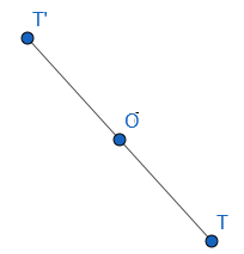
\includegraphics[scale=0.5]{Slike in skice/Zrcaljenje_tocke_cez_tocko.png}
            %     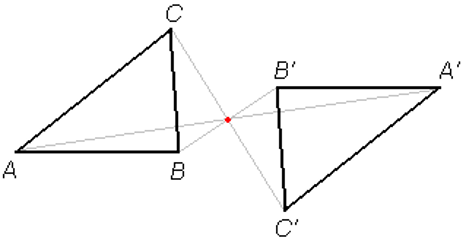
\includegraphics[scale=0.5]{Slike in skice/Zrcaljenje_lika_cez_tocko.png}
            % \end{figure}

            \begin{figure}
                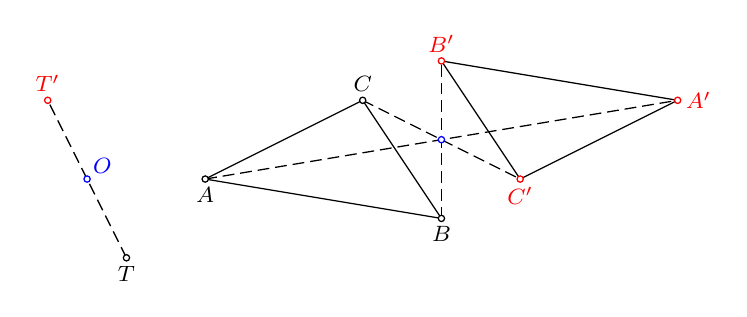
\begin{tikzpicture}
                    % \clip (0,0) rectangle (14.000000,10.000000);
                    {\footnotesize
                    
                    % Marking point T by circle
                    \draw [line width=0.016cm] (3.500000,1.500000) circle (0.040000);%
                    \draw (3.500000,1.500000) node [anchor=north] { $T$ };%
                    
                    % Drawing segment T T'
                    \draw [line width=0.016cm] (3.482111,1.535777) -- (3.432918,1.634164);%
                    \draw [line width=0.016cm] (3.399377,1.701246) -- (3.332295,1.835410);%
                    \draw [line width=0.016cm] (3.298754,1.902492) -- (3.231672,2.036656);%
                    \draw [line width=0.016cm] (3.198131,2.103738) -- (3.131049,2.237902);%
                    \draw [line width=0.016cm] (3.097508,2.304984) -- (3.030426,2.439149);%
                    \draw [line width=0.016cm] (2.982111,2.535777) -- (2.929803,2.640395);%
                    \draw [line width=0.016cm] (2.896262,2.707477) -- (2.829180,2.841641);%
                    \draw [line width=0.016cm] (2.795639,2.908723) -- (2.728557,3.042887);%
                    \draw [line width=0.016cm] (2.695016,3.109969) -- (2.627933,3.244133);%
                    \draw [line width=0.016cm] (2.594392,3.311215) -- (2.527310,3.445379);%
                    
                    % Drawing segment C C'
                    \draw [line width=0.016cm] (6.535777,3.482111) -- (6.634164,3.432918);%
                    \draw [line width=0.016cm] (6.701246,3.399377) -- (6.835410,3.332295);%
                    \draw [line width=0.016cm] (6.902492,3.298754) -- (7.036656,3.231672);%
                    \draw [line width=0.016cm] (7.103738,3.198131) -- (7.237902,3.131049);%
                    \draw [line width=0.016cm] (7.304984,3.097508) -- (7.439149,3.030426);%
                    \draw [line width=0.016cm] (7.535777,2.982111) -- (7.640395,2.929803);%
                    \draw [line width=0.016cm] (7.707477,2.896262) -- (7.841641,2.829180);%
                    \draw [line width=0.016cm] (7.908723,2.795639) -- (8.042887,2.728557);%
                    \draw [line width=0.016cm] (8.109969,2.695016) -- (8.244133,2.627933);%
                    \draw [line width=0.016cm] (8.311215,2.594392) -- (8.445379,2.527310);%
                    
                    % Drawing segment B B'
                    \draw [line width=0.016cm] (7.500000,2.040000) -- (7.500000,2.150000);%
                    \draw [line width=0.016cm] (7.500000,2.225000) -- (7.500000,2.375000);%
                    \draw [line width=0.016cm] (7.500000,2.450000) -- (7.500000,2.600000);%
                    \draw [line width=0.016cm] (7.500000,2.675000) -- (7.500000,2.825000);%
                    \draw [line width=0.016cm] (7.500000,2.900000) -- (7.500000,2.960000);%
                    \draw [line width=0.016cm] (7.500000,3.040000) -- (7.500000,3.050000);%
                    \draw [line width=0.016cm] (7.500000,3.125000) -- (7.500000,3.275000);%
                    \draw [line width=0.016cm] (7.500000,3.350000) -- (7.500000,3.500000);%
                    \draw [line width=0.016cm] (7.500000,3.575000) -- (7.500000,3.725000);%
                    \draw [line width=0.016cm] (7.500000,3.800000) -- (7.500000,3.950000);%
                    
                    % Drawing segment A A'
                    \draw [line width=0.016cm] (4.539456,2.506576) -- (4.647959,2.524660);%
                    \draw [line width=0.016cm] (4.721939,2.536990) -- (4.869898,2.561650);%
                    \draw [line width=0.016cm] (4.943877,2.573980) -- (5.091836,2.598639);%
                    \draw [line width=0.016cm] (5.165816,2.610969) -- (5.313775,2.635629);%
                    \draw [line width=0.016cm] (5.387755,2.647959) -- (5.535714,2.672619);%
                    \draw [line width=0.016cm] (5.609693,2.684949) -- (5.757652,2.709609);%
                    \draw [line width=0.016cm] (5.831632,2.721939) -- (5.979591,2.746598);%
                    \draw [line width=0.016cm] (6.053570,2.758928) -- (6.201530,2.783588);%
                    \draw [line width=0.016cm] (6.275509,2.795918) -- (6.423468,2.820578);%
                    \draw [line width=0.016cm] (6.497448,2.832908) -- (6.645407,2.857568);%
                    \draw [line width=0.016cm] (6.719386,2.869898) -- (6.867345,2.894558);%
                    \draw [line width=0.016cm] (6.941325,2.906887) -- (7.089284,2.931547);%
                    \draw [line width=0.016cm] (7.163264,2.943877) -- (7.311223,2.968537);%
                    \draw [line width=0.016cm] (7.385202,2.980867) -- (7.460544,2.993424);%
                    \draw [line width=0.016cm] (7.607141,3.017857) -- (7.755100,3.042517);%
                    \draw [line width=0.016cm] (7.829079,3.054847) -- (7.977039,3.079506);%
                    \draw [line width=0.016cm] (8.051018,3.091836) -- (8.198977,3.116496);%
                    \draw [line width=0.016cm] (8.272957,3.128826) -- (8.420916,3.153486);%
                    \draw [line width=0.016cm] (8.494895,3.165816) -- (8.642854,3.190476);%
                    \draw [line width=0.016cm] (8.716834,3.202806) -- (8.864793,3.227466);%
                    \draw [line width=0.016cm] (8.938773,3.239795) -- (9.086732,3.264455);%
                    \draw [line width=0.016cm] (9.160711,3.276785) -- (9.308670,3.301445);%
                    \draw [line width=0.016cm] (9.382650,3.313775) -- (9.530609,3.338435);%
                    \draw [line width=0.016cm] (9.604589,3.350765) -- (9.752548,3.375425);%
                    \draw [line width=0.016cm] (9.826527,3.387755) -- (9.974486,3.412414);%
                    \draw [line width=0.016cm] (10.048466,3.424744) -- (10.196425,3.449404);%
                    \draw [line width=0.016cm] (10.270404,3.461734) -- (10.418364,3.486394);%
                    
                    % Marking point C by circle
                    \draw [line width=0.016cm] (6.500000,3.500000) circle (0.040000);%
                    \draw (6.500000,3.500000) node [anchor=south] { $C$ };%
                    
                    % Marking point A by circle
                    \draw [line width=0.016cm] (4.500000,2.500000) circle (0.040000);%
                    \draw (4.500000,2.500000) node [anchor=north] { $A$ };%
                    
                    % Marking point B by circle
                    \draw [line width=0.016cm] (7.500000,2.000000) circle (0.040000);%
                    \draw (7.500000,2.000000) node [anchor=north] { $B$ };%
                    
                    % Drawing segment A B
                    \draw [line width=0.016cm] (4.539456,2.493424) -- (7.460544,2.006576);%
                    
                    % Drawing segment B C
                    \draw [line width=0.016cm] (7.477812,2.033282) -- (6.522188,3.466718);%
                    
                    % Drawing segment C A
                    \draw [line width=0.016cm] (6.464223,3.482111) -- (4.535777,2.517889);%
                    
                    % Drawing segment C' A'
                    \draw [line width=0.016cm] (8.535777,2.517889) -- (10.464223,3.482111);%
                    
                    % Drawing segment B' C'
                    \draw [line width=0.016cm] (7.522188,3.966718) -- (8.477812,2.533282);%
                    
                    % Drawing segment A' B'
                    \draw [line width=0.016cm] (10.460544,3.506576) -- (7.539456,3.993424);%
                    
                    % Changing color 0 0 255
                    \definecolor{r0g0b255}{rgb}{0.000000,0.000000,1.000000}%
                    \color{r0g0b255}% 
                    
                    % Marking point O by circle
                    \draw [line width=0.016cm] (3.000000,2.500000) circle (0.040000);%
                    \draw (2.970000,2.470000) node [anchor=south west] { $O$ };%
                    
                    % Marking point r by circle
                    \draw [line width=0.016cm] (7.500000,3.000000) circle (0.040000);%
                    
                    % Changing color 255 0 0
                    \definecolor{r255g0b0}{rgb}{1.000000,0.000000,0.000000}%
                    \color{r255g0b0}% 
                    
                    % Marking point T' by circle
                    \draw [line width=0.016cm] (2.500000,3.500000) circle (0.040000);%
                    \draw (2.500000,3.500000) node [anchor=south] { $T'$ };%
                    
                    % Marking point C' by circle
                    \draw [line width=0.016cm] (8.500000,2.500000) circle (0.040000);%
                    \draw (8.500000,2.500000) node [anchor=north] { $C'$ };%
                    
                    % Marking point B' by circle
                    \draw [line width=0.016cm] (7.500000,4.000000) circle (0.040000);%
                    \draw (7.500000,4.000000) node [anchor=south] { $B'$ };%
                    
                    % Marking point A' by circle
                    \draw [line width=0.016cm] (10.500000,3.500000) circle (0.040000);%
                    \draw (10.500000,3.500000) node [anchor=west] { $A'$ };%
                    \color{black}
                    }
                \end{tikzpicture}
                    
            \end{figure}

            Zrcaljenje čez točko daljice preslika v enako dolge daljice, ohranja velikosti kotov in orientacijo likov, like preslika v skladne like, premice preslika v vzporedne premice.

            \note{
                TABLA: konstrukcija zracljenja točke in trikotnika preko točke
                \\
                S pomočjo skic na tabli/okviru ugotavljanje lastnosti zrcaljenja preko točke.
            }
        \end{frame}



        \begin{frame}
            \large\textbf{Simetrija}
            ~\\
            \normalsize
            \begin{columns}
                \column{0.65\textwidth}
                ~\\
                Množica točk $\mathcal{M}$ je \textbf{simetrična/somerna glede na premico} $p$, če se pri zrcaljenju čez premico $p$ preslika sama vase. Premico $p$ imenujemo \textbf{simetrala}, \textbf{somernica}, \textbf{simetrijska os} množice $\mathcal{M}$. \\
                 ~\\      
                 ~\\      
                Množica točk $\mathcal{M}$ je \textbf{središčno simetrična/somerna glede na točko} $T$, če se pri zrcaljenju čez točko $T$ preslika sama vase. Točko $T$ imenujemo \textbf{center simetrije} množice $\mathcal{M}$. 
                \column{0.32\textwidth}
                \begin{figure}
                    % 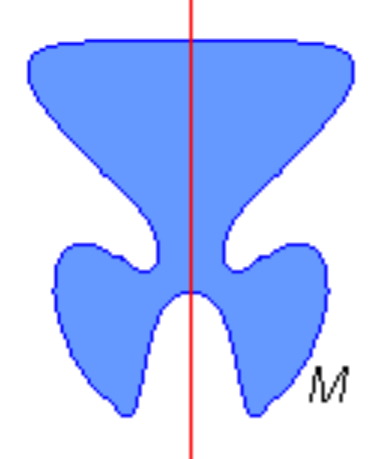
\includegraphics[scale=0.25]{../Slike in skice/Simetrija glede na premico.png}

                    % 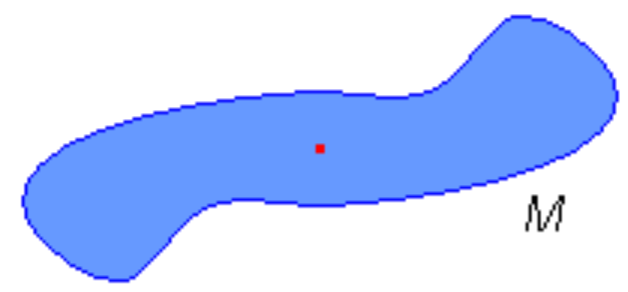
\includegraphics[scale=0.25]{../Slike in skice/Simetrija glede na točko.png}
                \end{figure}
            \end{columns}


            \note{
                Ponovitev definicije in konstrukcije simetrale daljice in simetrale kota.
            }
        \end{frame}

        \begin{frame}
            \large\textbf{Rotacija/vrtenje okoli točke}
            ~\\
            \normalsize
            \onslide<2->{
                \textbf{Vrtenje} ali \textbf{zasuk} oziroma \textbf{rotacija} za kot $\varphi$ okrog točke $O$ preslika točko $T$ v točko $T'$, da velja: $\left\lvert OT\right\rvert = \left\lvert OT'\right\rvert$  in $\angle TOT' = \varphi$.
            }

            % \begin{figure}
            %     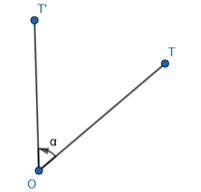
\includegraphics[scale=0.6]{Slike in skice/Rotacija tocke_okoli_tocke.png}
            %     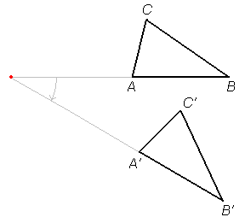
\includegraphics[scale=0.6]{Slike in skice/Rotacija_lika_okoli_tocke.png}
            % \end{figure}

            \pause
            \begin{figure}
                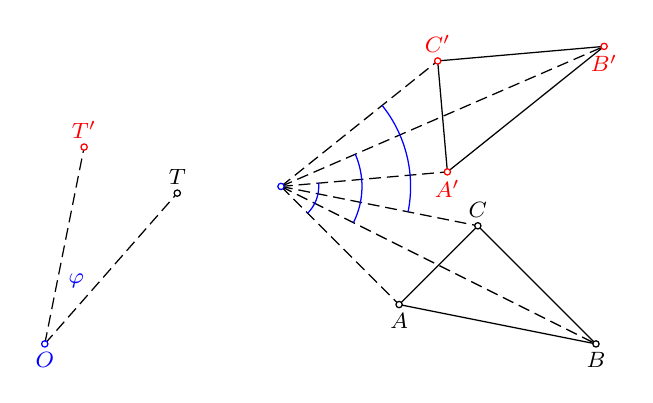
\begin{tikzpicture}
                    % \clip (0,0) rectangle (14.000000,10.000000);
                    {\footnotesize
                    
                    % Drawing segment O T
                    \draw<4-> [line width=0.016cm] (1.526405,1.530046) -- (1.599020,1.612672);%
                    \draw<4-> [line width=0.016cm] (1.648530,1.669009) -- (1.747550,1.781681);%
                    \draw<4-> [line width=0.016cm] (1.797059,1.838017) -- (1.896079,1.950690);%
                    \draw<4-> [line width=0.016cm] (1.945589,2.007026) -- (2.044609,2.119698);%
                    \draw<4-> [line width=0.016cm] (2.094119,2.176035) -- (2.193139,2.288707);%
                    \draw<4-> [line width=0.016cm] (2.242649,2.345043) -- (2.341668,2.457716);%
                    \draw<4-> [line width=0.016cm] (2.391178,2.514052) -- (2.490198,2.626724);%
                    \draw<4-> [line width=0.016cm] (2.539708,2.683060) -- (2.638728,2.795733);%
                    \draw<4-> [line width=0.016cm] (2.688238,2.852069) -- (2.787258,2.964742);%
                    \draw<4-> [line width=0.016cm] (2.836768,3.021078) -- (2.935787,3.133750);%
                    \draw<4-> [line width=0.016cm] (2.985297,3.190086) -- (3.084317,3.302759);%
                    \draw<4-> [line width=0.016cm] (3.133827,3.359095) -- (3.156608,3.385017);%
                    
                    % Drawing segment O T'
                    \draw<5-> [line width=0.016cm] (1.507845,1.539223) -- (1.529417,1.647087);%
                    \draw<5-> [line width=0.016cm] (1.544126,1.720631) -- (1.573544,1.867718);%
                    \draw<5-> [line width=0.016cm] (1.588252,1.941261) -- (1.617670,2.088348);%
                    \draw<5-> [line width=0.016cm] (1.632378,2.161892) -- (1.661796,2.308979);%
                    \draw<5-> [line width=0.016cm] (1.676505,2.382523) -- (1.705922,2.529610);%
                    \draw<5-> [line width=0.016cm] (1.720631,2.603153) -- (1.750048,2.750240);%
                    \draw<5-> [line width=0.016cm] (1.764757,2.823784) -- (1.794174,2.970871);%
                    \draw<5-> [line width=0.016cm] (1.808883,3.044415) -- (1.838300,3.191502);%
                    \draw<5-> [line width=0.016cm] (1.853009,3.265045) -- (1.882426,3.412132);%
                    \draw<5-> [line width=0.016cm] (1.897135,3.485676) -- (1.926553,3.632763);%
                    \draw<5-> [line width=0.016cm] (1.941261,3.706307) -- (1.970679,3.853394);%
                    \draw<5-> [line width=0.016cm] (1.985387,3.926937) -- (1.992155,3.960777);%
                    
                    % Marking point C by circle
                    \draw<6-> [line width=0.016cm] (7.000000,3.000000) circle (0.040000);%
                    \draw<6-> (7.000000,3.000000) node [anchor=south] { $C$ };%
                    
                    % Marking point A by circle
                    \draw<6-> [line width=0.016cm] (6.000000,2.000000) circle (0.040000);%
                    \draw<6-> (6.000000,2.000000) node [anchor=north] { $A$ };%
                    
                    % Marking point B by circle
                    \draw<6-> [line width=0.016cm] (8.500000,1.500000) circle (0.040000);%
                    \draw<6-> (8.500000,1.500000) node [anchor=north] { $B$ };%
                    
                    % Drawing segment A B
                    \draw<6-> [line width=0.016cm] (6.039223,1.992155) -- (8.460777,1.507845);%
                    
                    % Drawing segment B C
                    \draw<6-> [line width=0.016cm] (8.471716,1.528284) -- (7.028284,2.971716);%
                    
                    % Drawing segment A C
                    \draw<6-> [line width=0.016cm] (6.028284,2.028284) -- (6.971716,2.971716);%
                    
                    % Drawing segment X A
                    \draw<7-> [line width=0.016cm] (4.528284,3.471716) -- (4.606066,3.393934);%
                    \draw<7-> [line width=0.016cm] (4.659099,3.340901) -- (4.765165,3.234835);%
                    \draw<7-> [line width=0.016cm] (4.818198,3.181802) -- (4.924264,3.075736);%
                    \draw<7-> [line width=0.016cm] (4.977297,3.022703) -- (5.083363,2.916637);%
                    \draw<7-> [line width=0.016cm] (5.136396,2.863604) -- (5.242462,2.757538);%
                    \draw<7-> [line width=0.016cm] (5.295495,2.704505) -- (5.401561,2.598439);%
                    \draw<7-> [line width=0.016cm] (5.454594,2.545406) -- (5.560660,2.439340);%
                    \draw<7-> [line width=0.016cm] (5.613693,2.386307) -- (5.719759,2.280241);%
                    \draw<7-> [line width=0.016cm] (5.772792,2.227208) -- (5.878858,2.121142);%
                    \draw<7-> [line width=0.016cm] (5.931891,2.068109) -- (5.971716,2.028284);%
                    
                    % Drawing segment X B
                    \draw<7-> [line width=0.016cm] (4.535777,3.482111) -- (4.634164,3.432918);%
                    \draw<7-> [line width=0.016cm] (4.701246,3.399377) -- (4.835410,3.332295);%
                    \draw<7-> [line width=0.016cm] (4.902492,3.298754) -- (5.036656,3.231672);%
                    \draw<7-> [line width=0.016cm] (5.103738,3.198131) -- (5.237902,3.131049);%
                    \draw<7-> [line width=0.016cm] (5.304984,3.097508) -- (5.439149,3.030426);%
                    \draw<7-> [line width=0.016cm] (5.506231,2.996885) -- (5.640395,2.929803);%
                    \draw<7-> [line width=0.016cm] (5.707477,2.896262) -- (5.841641,2.829180);%
                    \draw<7-> [line width=0.016cm] (5.908723,2.795639) -- (6.042887,2.728557);%
                    \draw<7-> [line width=0.016cm] (6.109969,2.695016) -- (6.244133,2.627933);%
                    \draw<7-> [line width=0.016cm] (6.311215,2.594392) -- (6.445379,2.527310);%
                    \draw<7-> [line width=0.016cm] (6.512461,2.493769) -- (6.646625,2.426687);%
                    \draw<7-> [line width=0.016cm] (6.713707,2.393146) -- (6.847871,2.326064);%
                    \draw<7-> [line width=0.016cm] (6.914953,2.292523) -- (7.049117,2.225441);%
                    \draw<7-> [line width=0.016cm] (7.116200,2.191900) -- (7.250364,2.124818);%
                    \draw<7-> [line width=0.016cm] (7.317446,2.091277) -- (7.451610,2.024195);%
                    \draw<7-> [line width=0.016cm] (7.518692,1.990654) -- (7.652856,1.923572);%
                    \draw<7-> [line width=0.016cm] (7.719938,1.890031) -- (7.854102,1.822949);%
                    \draw<7-> [line width=0.016cm] (7.921184,1.789408) -- (8.055348,1.722326);%
                    \draw<7-> [line width=0.016cm] (8.122430,1.688785) -- (8.256594,1.621703);%
                    \draw<7-> [line width=0.016cm] (8.323676,1.588162) -- (8.457840,1.521080);%
                    
                    % Drawing segment X C
                    \draw<7-> [line width=0.016cm] (4.539223,3.492155) -- (4.647087,3.470583);%
                    \draw<7-> [line width=0.016cm] (4.720631,3.455874) -- (4.867718,3.426456);%
                    \draw<7-> [line width=0.016cm] (4.941261,3.411748) -- (5.088348,3.382330);%
                    \draw<7-> [line width=0.016cm] (5.161892,3.367622) -- (5.308979,3.338204);%
                    \draw<7-> [line width=0.016cm] (5.382523,3.323495) -- (5.529610,3.294078);%
                    \draw<7-> [line width=0.016cm] (5.603153,3.279369) -- (5.750240,3.249952);%
                    \draw<7-> [line width=0.016cm] (5.823784,3.235243) -- (5.970871,3.205826);%
                    \draw<7-> [line width=0.016cm] (6.044415,3.191117) -- (6.191502,3.161700);%
                    \draw<7-> [line width=0.016cm] (6.265045,3.146991) -- (6.412132,3.117574);%
                    \draw<7-> [line width=0.016cm] (6.485676,3.102865) -- (6.632763,3.073447);%
                    \draw<7-> [line width=0.016cm] (6.706307,3.058739) -- (6.853394,3.029321);%
                    \draw<7-> [line width=0.016cm] (6.926937,3.014613) -- (6.960777,3.007845);%
                    
                    % Drawing segment A' B'
                    \draw<10-> [line width=0.016cm] (6.644470,3.709889) -- (8.572018,5.253598);%
                    
                    % Drawing segment B' C'
                    \draw<10-> [line width=0.016cm] (8.563392,5.275116) -- (6.529839,5.097203);%
                    
                    % Drawing segment A' C'
                    \draw<10-> [line width=0.016cm] (6.609762,3.724733) -- (6.493478,5.053869);%
                    
                    % Drawing segment X A'
                    \draw<8-> [line width=0.016cm] (4.539848,3.503486) -- (4.649429,3.513073);%
                    \draw<8-> [line width=0.016cm] (4.724144,3.519610) -- (4.873573,3.532683);%
                    \draw<8-> [line width=0.016cm] (4.948288,3.539220) -- (5.097717,3.552293);%
                    \draw<8-> [line width=0.016cm] (5.172431,3.558830) -- (5.321861,3.571903);%
                    \draw<8-> [line width=0.016cm] (5.396575,3.578440) -- (5.546004,3.591513);%
                    \draw<8-> [line width=0.016cm] (5.620719,3.598050) -- (5.770148,3.611124);%
                    \draw<8-> [line width=0.016cm] (5.844863,3.617660) -- (5.994292,3.630734);%
                    \draw<8-> [line width=0.016cm] (6.069007,3.637270) -- (6.218436,3.650344);%
                    \draw<8-> [line width=0.016cm] (6.293150,3.656880) -- (6.442580,3.669954);%
                    \draw<8-> [line width=0.016cm] (6.517294,3.676490) -- (6.573400,3.681399);%
                    
                    % Drawing segment X B'
                    \draw<8-> [line width=0.016cm] (4.536700,3.515908) -- (4.637627,3.559656);%
                    \draw<8-> [line width=0.016cm] (4.706440,3.589484) -- (4.844067,3.649140);%
                    \draw<8-> [line width=0.016cm] (4.912881,3.678968) -- (5.050507,3.738625);%
                    \draw<8-> [line width=0.016cm] (5.119321,3.768453) -- (5.256948,3.828109);%
                    \draw<8-> [line width=0.016cm] (5.325761,3.857937) -- (5.463388,3.917593);%
                    \draw<8-> [line width=0.016cm] (5.532201,3.947421) -- (5.669828,4.007077);%
                    \draw<8-> [line width=0.016cm] (5.738642,4.036905) -- (5.876268,4.096561);%
                    \draw<8-> [line width=0.016cm] (5.945082,4.126389) -- (6.082709,4.186046);%
                    \draw<8-> [line width=0.016cm] (6.151522,4.215874) -- (6.289149,4.275530);%
                    \draw<8-> [line width=0.016cm] (6.357962,4.305358) -- (6.495589,4.365014);%
                    \draw<8-> [line width=0.016cm] (6.564403,4.394842) -- (6.702029,4.454498);%
                    \draw<8-> [line width=0.016cm] (6.770843,4.484326) -- (6.908470,4.543982);%
                    \draw<8-> [line width=0.016cm] (6.977283,4.573810) -- (7.114910,4.633467);%
                    \draw<8-> [line width=0.016cm] (7.183723,4.663295) -- (7.321350,4.722951);%
                    \draw<8-> [line width=0.016cm] (7.390164,4.752779) -- (7.527790,4.812435);%
                    \draw<8-> [line width=0.016cm] (7.596604,4.842263) -- (7.734231,4.901919);%
                    \draw<8-> [line width=0.016cm] (7.803044,4.931747) -- (7.940671,4.991403);%
                    \draw<8-> [line width=0.016cm] (8.009484,5.021232) -- (8.147111,5.080888);%
                    \draw<8-> [line width=0.016cm] (8.215925,5.110716) -- (8.353551,5.170372);%
                    \draw<8-> [line width=0.016cm] (8.422365,5.200200) -- (8.559992,5.259856);%
                    
                    % Drawing segment X C'
                    \draw<8-> [line width=0.016cm] (4.531222,3.525004) -- (4.617081,3.593766);%
                    \draw<8-> [line width=0.016cm] (4.675621,3.640649) -- (4.792702,3.734415);%
                    \draw<8-> [line width=0.016cm] (4.851242,3.781298) -- (4.968323,3.875064);%
                    \draw<8-> [line width=0.016cm] (5.026864,3.921947) -- (5.143945,4.015714);%
                    \draw<8-> [line width=0.016cm] (5.202485,4.062597) -- (5.319566,4.156363);%
                    \draw<8-> [line width=0.016cm] (5.378106,4.203246) -- (5.495187,4.297012);%
                    \draw<8-> [line width=0.016cm] (5.553727,4.343895) -- (5.670808,4.437661);%
                    \draw<8-> [line width=0.016cm] (5.729349,4.484544) -- (5.846429,4.578310);%
                    \draw<8-> [line width=0.016cm] (5.904970,4.625193) -- (6.022051,4.718959);%
                    \draw<8-> [line width=0.016cm] (6.080591,4.765842) -- (6.197672,4.859608);%
                    \draw<8-> [line width=0.016cm] (6.256212,4.906491) -- (6.373293,5.000258);%
                    \draw<8-> [line width=0.016cm] (6.431834,5.047141) -- (6.458770,5.068713);%
                    
                    % Marking point T by circle
                    \draw<3-> [line width=0.016cm] (3.183013,3.415063) circle (0.040000);%
                    \draw<3-> (3.183013,3.415063) node [anchor=south] { $T$ };%
                    
                    % Changing color 0 0 255
                    \definecolor{r0g0b255}{rgb}{0.000000,0.000000,1.000000}%
                    \color{r0g0b255}% 
                    
                    % Marking point O by circle
                    \draw<3-> [line width=0.016cm] (1.500000,1.500000) circle (0.040000);%
                    \draw<3-> (1.500000,1.500000) node [anchor=north] { $O$ };%
                    
                    % Marking point \alpha
                    \draw<5-> (1.900000,2.300000) node  { $\varphi$ };%
                    
                    % Marking point X by circle
                    \draw<6-> [line width=0.016cm] (4.500000,3.500000) circle (0.040000);%
                    
                    % Drawing arc X a 50.00
                    \draw<8-> [line width=0.016cm] (4.839000,3.161000) -- (4.839000,3.161000) arc (315:360:0.479418 and 0.479418) --(4.979418,3.500000) arc (0:4:0.479418 and 0.479418) -- (4.977594,3.541784);%
                    
                    % Drawing arc X b 50.00
                    \draw<8-> [line width=0.016cm] (5.420000,3.040000) -- (5.424492,3.049095) arc (334:360:1.028591 and 1.028591) --(5.528591,3.500000) arc (0:23:1.028591 and 1.028591) -- (5.443745,3.909079);%
                    
                    % Drawing arc X c 50.00
                    \draw<8-> [line width=0.016cm] (6.114000,3.177000) -- (6.115761,3.185927) arc (349:360:1.646003 and 1.646003) --(6.146003,3.500000) arc (0:38:1.646003 and 1.646003) -- (5.784892,4.528775);%
                    
                    % Changing color 255 0 0
                    \definecolor{r255g0b0}{rgb}{1.000000,0.000000,0.000000}%
                    \color{r255g0b0}% 
                    
                    % Marking point T' by circle
                    \draw<5-> [line width=0.016cm] (2.000000,4.000000) circle (0.040000);%
                    \draw<5-> (2.000000,4.000000) node [anchor=south] { $T'$ };%
                    
                    % Marking point A' by circle
                    \draw<9-> [line width=0.016cm] (6.613248,3.684885) circle (0.040000);%
                    \draw<9-> (6.613248,3.684885) node [anchor=north] { $A'$ };%
                    
                    % Marking point B' by circle
                    \draw<9-> [line width=0.016cm] (8.603239,5.278602) circle (0.040000);%
                    \draw<9-> (8.603239,5.278602) node [anchor=north] { $B'$ };%
                    
                    % Marking point C' by circle
                    \draw<9-> [line width=0.016cm] (6.489991,5.093717) circle (0.040000);%
                    \draw<9-> (6.489991,5.093717) node [anchor=south] { $C'$ };%
                    \color{black}
                    }
                \end{tikzpicture}
            \end{figure}

            \onslide<11->{Vrtenje okoli točke preslika daljice v enako dolge daljice, ohranja velikosti kotov in orientacijo likov, like preslika v skladne like, premic pa ne preslika v vzporedne premice.} 


            \note{
                TABLA: konstrukcija rotacije točke okoli točke za nek kot; rotacija trikotnika za isti kot
                \\
                Opomba: vrtenje v pozitivni/negativni smeri oziroma za pozitiven/negativen kot
                \\
                S pomočjo skic na tabli/okviru ugotovitev lastnosti dane prelikave.

            }
        \end{frame}


        % \begin{frame}

        %     \begin{exampleblock}{Naloga}
        %         Konstruiraj daljico $AB$ poljubne dolžine. Konstruiraj še:
        %         \begin{itemize}
        %             \item točko $C$, ki jo dobiš tako, da točko $B$ zavrtiš okrog točke $A$ za kot $120^\circ$;
        %             \item točko $D$, ki je pravokotna projekcija točke $C$ na nosilko daljice $AB$;
        %             \item zrcalno sliko točke $C$ glede na točko $B$ in dobljeno točko označi $C'$;
        %             \item simetralo kota z vrhom v $B$, katerega kraka potekata skozi $C$ in $C'$.
        %         \end{itemize}
        %     \end{exampleblock}

        % \end{frame}
        % \note{
        %     Priredba nalog 57 in 58 v Matematika 2 (Zbirka nalog ...).
        % }







        

        %%%%%%%% naloge

        \begin{frame}
            \only<2->{\begin{exampleblock}{Naloga}
                Narišite kvadrat s stranico dolžine $1$ in ga:
                \begin{itemize}
                    \item vzporedno premaknite vzdolž ordinatne osi za $3$ enota;
                    \item zavrtite okrog oglišča $B$ za kot $45^\circ$ v negativni smeri;
                    \item zrcalite preko nosilke stranice $CD$.
                \end{itemize}
            \end{exampleblock}}

            \only<3->{\begin{exampleblock}{Naloga}
                Izračunajte velikosti kotov $\alpha$, $\beta$ in $\gamma$. Podatke razberite iz skic. Velja $p\parallel q$ in $r\parallel s$.
                \begin{figure}
                    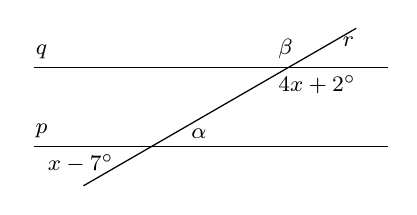
\begin{tikzpicture}
                        % \clip (0,0) rectangle (14.000000,10.000000);
                        {\footnotesize

                        % Drawing line Q
                        \draw [line width=0.016cm] (1.500000,1.500000) -- (6.000000,1.500000);%

                        % Drawing line P
                        \draw [line width=0.016cm] (1.500000,2.500000) -- (6.000000,2.500000);%

                        % Drawing line R
                        \draw [line width=0.016cm] (2.133975,1.000000) -- (5.598076,3.000000);%

                        % Marking point p
                        \draw (1.600000,1.500000) node [anchor=south] { $p$ };%

                        % Marking point q
                        \draw (1.600000,2.500000) node [anchor=south] { $q$ };%

                        % Marking point r
                        \draw (5.500000,3.000000) node [anchor=north] { $r$ };%

                        % Marking point \alpha
                        \draw (3.600000,1.500000) node [anchor=south] { $\alpha$ };%

                        % Marking point \beta
                        \draw (4.700000,2.500000) node [anchor=south] { $\beta$ };%

                        % Marking point {4x+2^\circ}
                        \draw (5.100000,2.500000) node [anchor=north] { ${4x+2^\circ}$ };%

                        % Marking point {x-7^\circ}
                        \draw (2.100000,1.500000) node [anchor=north] { ${x-7^\circ}$ };%
                        }
                    \end{tikzpicture} ~
                    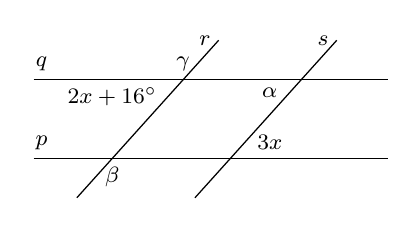
\begin{tikzpicture}
                        % \clip (0,0) rectangle (14.000000,10.000000);
                        {\footnotesize

                        % Drawing line Q
                        \draw [line width=0.016cm] (1.500000,1.500000) -- (6.000000,1.500000);%

                        % Drawing line P
                        \draw [line width=0.016cm] (1.500000,2.500000) -- (6.000000,2.500000);%

                        % Drawing line R
                        \draw [line width=0.016cm] (2.049798,1.000000) -- (3.850606,3.000000);%

                        % Drawing line S
                        \draw [line width=0.016cm] (3.549798,1.000000) -- (5.350606,3.000000);%

                        % Marking point p
                        \draw (1.600000,1.500000) node [anchor=south] { $p$ };%

                        % Marking point q
                        \draw (1.600000,2.500000) node [anchor=south] { $q$ };%

                        % Marking point r
                        \draw (3.500000,3.000000) node [anchor=west] { $r$ };%

                        % Marking point s
                        \draw (5.000000,3.000000) node [anchor=west] { $s$ };%

                        % Marking point \alpha
                        \draw (4.500000,2.500000) node [anchor=north] { $\alpha$ };%

                        % Marking point \beta
                        \draw (2.500000,1.500000) node [anchor=north] { $\beta$ };%

                        % Marking point \gamma
                        \draw (3.400000,2.500000) node [anchor=south] { $\gamma$ };%

                        % Marking point {3x}
                        \draw (4.500000,1.500000) node [anchor=south] { ${3x}$ };%

                        % Marking point {2x+16^\circ}
                        \draw (2.500000,2.500000) node [anchor=north] { ${2x+16^\circ}$ };%
                        }
                    \end{tikzpicture} ~
                    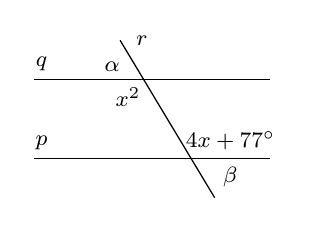
\begin{tikzpicture}
                        % \clip (0,0) rectangle (14.000000,10.000000);
                        {\footnotesize

                        % Drawing line Q
                        \draw [line width=0.016cm] (1.500000,1.500000) -- (4.500000,1.500000);%

                        % Drawing line P
                        \draw [line width=0.016cm] (1.500000,2.500000) -- (4.500000,2.500000);%

                        % Drawing line R
                        \draw [line width=0.016cm] (3.800430,1.000000) -- (2.598709,3.000000);%

                        % Marking point p
                        \draw (1.600000,1.500000) node [anchor=south] { $p$ };%

                        % Marking point q
                        \draw (1.600000,2.500000) node [anchor=south] { $q$ };%

                        % Marking point r
                        \draw (2.700000,3.000000) node [anchor=west] { $r$ };%

                        % Marking point \alpha
                        \draw (2.500000,2.500000) node [anchor=south] { $\alpha$ };%

                        % Marking point \beta
                        \draw (4.000000,1.500000) node [anchor=north] { $\beta$ };%

                        % Marking point {4x+77^\circ}
                        \draw (4.000000,1.500000) node [anchor=south] { ${4x+77^\circ}$ };%

                        % Marking point {x^2}
                        \draw (2.700000,2.500000) node [anchor=north] { ${x^2}$ };%
                        }
                    \end{tikzpicture}
                \end{figure}
            \end{exampleblock}}
        \end{frame}

        \begin{frame}
            \only<2->{\begin{exampleblock}{Naloga}
                Izračunajte velikosti vseh notranjih in zunanjih kotov trikotnika $\triangle ABC$, 
                če je vsota velikosti dveh zunanjih kotov $\alpha'+\gamma'=230^\circ$, vsota velikosti dveh notranjih kotov pa $\alpha+\beta=70^\circ$.
            \end{exampleblock}}

            \only<3->{\begin{exampleblock}{Naloga}
                S skice preberite ustrezne podatke ter izračunajte velikosti kotov $\alpha$, $\beta$, $\gamma$ in $\delta$.
                Pri tem velja, da so premice $p$, $q$ in $r$ vzporedne.
                \begin{figure}
                    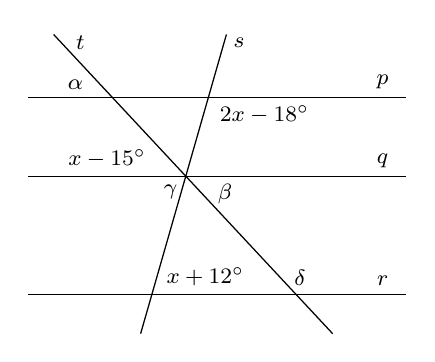
\begin{tikzpicture}
                        % \clip (0,0) rectangle (14.000000,10.000000);
                        {\footnotesize

                        % Drawing line Q
                        \draw [line width=0.016cm] (1.000000,3.000000) -- (5.800000,3.000000);%

                        % Drawing line P
                        \draw [line width=0.016cm] (1.000000,4.000000) -- (5.800000,4.000000);%

                        % Drawing line R
                        \draw [line width=0.016cm] (1.000000,1.500000) -- (5.800000,1.500000);%

                        % Drawing line S
                        \draw [line width=0.016cm] (2.426509,1.000000) -- (3.516142,4.800000);%

                        % Drawing line T
                        \draw [line width=0.016cm] (4.865030,1.000000) -- (1.321473,4.800000);%

                        % Marking point p
                        \draw (5.500000,4.000000) node [anchor=south] { $p$ };%

                        % Marking point q
                        \draw (5.500000,3.000000) node [anchor=south] { $q$ };%

                        % Marking point r
                        \draw (5.500000,1.500000) node [anchor=south] { $r$ };%

                        % Marking point s
                        \draw (3.500000,4.700000) node [anchor=west] { $s$ };%

                        % Marking point t
                        \draw (1.500000,4.700000) node [anchor=west] { $t$ };%

                        % Marking point \alpha
                        \draw (1.800000,4.000000) node [anchor=south east] { $\alpha$ };%

                        % Marking point \beta
                        \draw (3.300000,3.000000) node [anchor=north west] { $\beta$ };%

                        % Marking point \gamma
                        \draw (3.000000,3.000000) node [anchor=north east] { $\gamma$ };%

                        % Marking point \delta
                        \draw (4.450000,1.500000) node [anchor=south] { $\delta$ };%

                        % Marking point {x-15^\circ}
                        \draw (2.000000,3.000000) node [anchor=south] { ${x-15^\circ}$ };%

                        % Marking point {2x-18^\circ}
                        \draw (4.000000,4.000000) node [anchor=north] { ${2x-18^\circ}$ };%

                        % Marking point {x+12^\circ}
                        \draw (3.250000,1.500000) node [anchor=south] { ${x+12^\circ}$ };%
                        }
                    \end{tikzpicture}

                \end{figure}
            \end{exampleblock}}

        \end{frame}





%%%%%%%%%%%%%%%%%%%%%%%%%%%%%%%%

    \subsection{Trikotnik}

        \begin{frame}
            \frametitle{Trikotnik}

            \pause
            \begin{alertblock}{}
                \textbf{Trikotnik} je lik/množica točk v ravnini, omejena s tremi daljicami -- \textbf{stranice} ($a, b, c$), ki povezujejo tri nekolinearne točke ($A, B, C$) v ravnini. Te točke imenujemo \textbf{oglišča} trikotnika.
            \end{alertblock}
            
            % \begin{figure}
            %     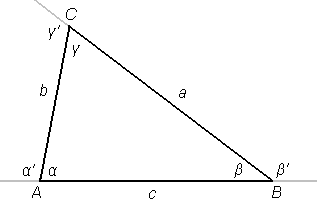
\includegraphics[scale=0.7]{Slike in skice/Trikotnik.png}    
            % \end{figure}

            \begin{figure}
                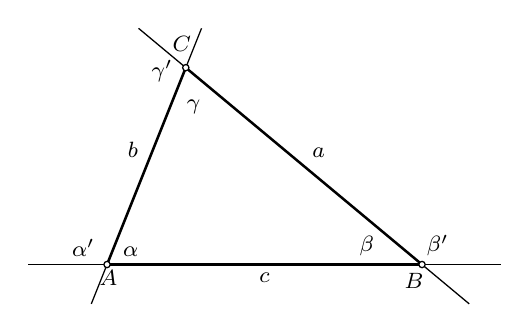
\begin{tikzpicture}
                    % \clip (0,0) rectangle (14.000000,10.000000);
                    {\footnotesize
                    
                    % Marking point A by circle
                    \draw<2-> [line width=0.016cm] (2.000000,1.500000) circle (0.040000);%
                    \draw<2-> (1.800000,1.530000) node [anchor=north west] { $A$ };%
                    
                    % Marking point B by circle
                    \draw<2-> [line width=0.016cm] (6.000000,1.500000) circle (0.040000);%
                    \draw<2-> (5.900000,1.500000) node [anchor=north] { $B$ };%
                    
                    % Marking point C by circle
                    \draw<2-> [line width=0.016cm] (3.000000,4.000000) circle (0.040000);%
                    \draw<2-> (2.950000,4.100000) node [anchor=south] { $C$ };%
                    
                    % Drawing line A B
                    \draw<4-> [line width=0.016cm] (1.000000,1.500000) -- (1.960000,1.500000);%
                    \draw<4-> [line width=0.016cm] (2.040000,1.500000) -- (5.960000,1.500000);%
                    \draw<4-> [line width=0.016cm] (6.040000,1.500000) -- (7.000000,1.500000);%
                    
                    % Drawing line B C
                    \draw<4-> [line width=0.016cm] (6.600000,1.000000) -- (6.030729,1.474393);%
                    \draw<4-> [line width=0.016cm] (5.969271,1.525607) -- (3.030729,3.974393);%
                    \draw<4-> [line width=0.016cm] (2.969271,4.025607) -- (2.400000,4.500000);%
                    
                    % Drawing line A C
                    \draw<4-> [line width=0.016cm] (1.800000,1.000000) -- (1.985144,1.462861);%
                    \draw<4-> [line width=0.016cm] (2.014856,1.537139) -- (2.985144,3.962861);%
                    \draw<4-> [line width=0.016cm] (3.014856,4.037139) -- (3.200000,4.500000);%
                    
                    % Marking point c
                    \draw<2-> (4.000000,1.500000) node [anchor=north] { $c$ };%
                    
                    % Marking point a
                    \draw<2-> (4.500000,2.750000) node [anchor=south west] { $a$ };%
                    
                    % Marking point b
                    \draw<2-> (2.500000,2.750000) node [anchor=south east] { $b$ };%
                    
                    % Marking point \gamma
                    \draw<3-> (3.100000,3.700000) node [anchor=north] { $\gamma$ };%
                    
                    % Marking point \gamma'
                    \draw<4-> (2.700000,4.200000) node [anchor=north] { $\gamma'$ };%
                    
                    % Marking point \beta
                    \draw<3-> (5.300000,1.500000) node [anchor=south] { $\beta$ };%
                    
                    % Marking point \beta'
                    \draw<4-> (6.200000,1.500000) node [anchor=south] { $\beta'$ };%
                    
                    % Marking point \alpha
                    \draw<3-> (2.300000,1.500000) node [anchor=south] { $\alpha$ };%
                    
                    % Marking point \alpha'
                    \draw<4-> (1.700000,1.500000) node [anchor=south] { $\alpha'$ };%
                    
                    % Drawing segment A B
                    \draw<2-> [line width=0.032cm] (2.040000,1.500000) -- (5.960000,1.500000);%
                    
                    % Drawing segment B C
                    \draw<2-> [line width=0.032cm] (5.969271,1.525607) -- (3.030729,3.974393);%
                    
                    % Drawing segment A C
                    \draw<2-> [line width=0.032cm] (2.014856,1.537139) -- (2.985144,3.962861);%
                    }
                \end{tikzpicture}
            \end{figure}

            \onslide<3->{V trikotniku $\triangle ABC$  so $\alpha, \beta$ in $\gamma$ \textbf{notranji koti},} \onslide<4->{njihovi sokoti $\alpha', \beta'$ in $\gamma'$ pa so \textbf{zunanji koti}. }
            

        \end{frame}


        \begin{frame}
            
            \begin{alertblock}{}
                Vsota notranjih kotov trikotnika je $180^\circ$: $$\alpha+\beta+\gamma=180^\circ.$$ 
            \end{alertblock}

            \pause
            \begin{alertblock}{}
                Zunanji kot trikotnika je enak vsoti notranjih nepriležnih kotov: 
                \begin{align*}
                    \alpha' &= \beta+\gamma \\
                    \beta' &= \alpha+\gamma \\
                    \gamma' &= \alpha+\beta
                \end{align*}
            \end{alertblock}

            \pause
            \begin{alertblock}{}
                Vsota zunanjih kotov trikotnika je $360^\circ$: $$\alpha'+\beta'+\gamma'=360^\circ.$$ 
            \end{alertblock}


            \note{
                DOKAZ 1. izreka: Upoštevamo lastnosti kotov z vzporednimi kraki. Narišemo nosilko stranice $a$ preko oglišča $C$. Konstruiramo vzpordnico k $c$ skozi $C$. Dobljena kota sta skladna $\alpha$ oziroma $\beta$. Vsi trije koti skupaj tvorijo iztegnjeni kot ($180^\circ$).
                \\
                DOKAZ 2. izreka: Dokaz naredimo zgolj za enega izmed kotov: Na skici dokaz prejšnjega izreka vidimo, da je zunanji kot pri oglišču $C$ enak vsoti kotov $\alpha$ in $\beta$.
                \\
                DOKAZ 3. izreka: Po prejšnjih dveh izrekih sledi, da je $\alpha'+\beta'+\gamma'=2\cdot(\alpha+\beta+\gamma)=2\cdot180^\circ=360^\circ$.
            }
        \end{frame}


        % \begin{frame}
        %     \begin{exampleblock}{Naloga 65}
        %         Izračunaj velikosti notranjih in zunanjih kotov trikotnika $\triangle ABC$, če je $\alpha= 67^\circ 13'$ in $\beta' = 133^\circ 25'$.
        %     \end{exampleblock}

        %     \pause
        %     \begin{exampleblock}{Naloga 68}
        %         Velikosti notranjih kotov trikotnika so v razmerju $2:5:11$. V kolikšnem razmerju so velikosti zunanjih kotov tega trikotnika?
        %     \end{exampleblock}

        %     \pause
        %     \begin{exampleblock}{Naloga 70}
        %         Notranji kot ob oglišču $A$ trikotnika $\triangle ABC$ je za $1^\circ$ manjši od velikosti notranjega kota ob oglišču $C$.  Zunanji kot v oglišču $C$ je za $1^\circ$ večji od dvakratnika velikosti notranjega kota ob oglišču $A$. Izračunaj velikosti notranjih kotov trikotnika $\triangle ABC$.
        %     \end{exampleblock}
        % \end{frame}
        

        \begin{frame}
            
            \begin{alertblock}{}
                Nasproti daljše stranice trikotnika leži večji notranji kot, nasproti krajše stranice pa manjši notranji kot trikotnika.
                $$a>b \Leftrightarrow \alpha > \beta$$
            \end{alertblock}

            \pause
            \begin{alertblock}{Trikotniška neenakost}
                Vsaka stranica trikotnika je krajša od vsote dolžin drugih dveh stranic.
                \begin{align*}
                    a &< b + c \\
                    b &< a + c \\
                    c &< a + b
                \end{align*}
            \end{alertblock}

            % \begin{alertblock}{}
            %     Vsaka stranica trikotnika je daljša od absolutne vrednosti razlike dolžin drugih dveh stranic.
            % \end{alertblock}


            \note{
                DOKAZ 1. izreka: Denimo, da je $c$ daljša od $b$ v trikotniku $ABC$. Konstruiramo simetralo $\alpha$ in označimo presečišče z $a$ z $D$. Daljico $AC$ prenesemo na $AB$ in točko označimo z $E$. Dobili smo skladna trikotnika $AED$ in $ACD$ (skupna $AD$, $|AC|=|AE|$, kot med njima). Torej je $\angle DEA = \gamma$ zunanji kot za trikotnik $EBD$, torej enak vsoti $\beta$ in $\angle EDB$. To pomeni da velja $\gamma > \beta$.
                \\
                DOKAZ 2. izreka: Dokaz naredimo zgolj za eno neenakost: Podaljšamo eno izmed stranic trikotnika $ABC$, naj bo to $a$, preko oglišča $C$ za dolžino stranice $b$. Dobili smo enakokrak trikotnik $ACC'$, skladna kota $\angle CAC'$ in $\angle AC'C$ označimo z $\varphi$. Kot $\angle BAC' = \epsilon$ je večji od $\varphi$. V trikotniku $ABC'$ je $\epsilon > \varphi$, zato je $BC' > c$. To nam da: $c<a+b$.
            }
        \end{frame}


        % \begin{frame}
        %     \begin{exampleblock}{Naloga 76}
        %         Ali obstaja trikotnik z danimi dolžinami stranic?
        %         \begin{enumerate}
        %             \item $a=4~cm,\ b=5~cm,\ c=10~cm$;
        %             \item $a=4~cm,\ b=5~cm,\ c=8~cm$;
        %             \item $a=5~cm,\ b=12~cm,\ c=6~cm$.
        %         \end{enumerate}
        %     \end{exampleblock}

        %     \pause
        %     \begin{exampleblock}{Naloga 77}
        %         Po velikosti uredi notranje kote trikotnika $\triangle ABC$.
        %         \begin{enumerate}
        %             \item $a=33~dm,\ b=22~dm,\ c=28~dm$;
        %             \item $a=32~m,\ b=35~m,\ c=38~m$;
        %         \end{enumerate}
        %     \end{exampleblock}

        % \end{frame}


        \begin{frame}

            \begin{alertblock}{}
                \textbf{Višina} na stranico trikotnika je daljica, ki povezuje nosilko te stranice z nasprotnim ogliščem in je pravokotna na to nosilko. 
                Njena dolžina je razdalja oglišča od nasprotne stranice.
            \end{alertblock}

            % \begin{figure}
            %     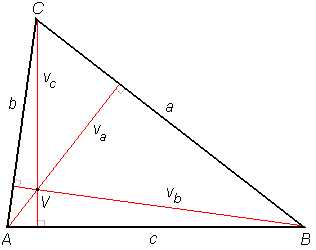
\includegraphics[scale=0.5]{Slike in skice/Visina_in_visinska_tocka.png}
            % \end{figure}
            
            \begin{figure}
                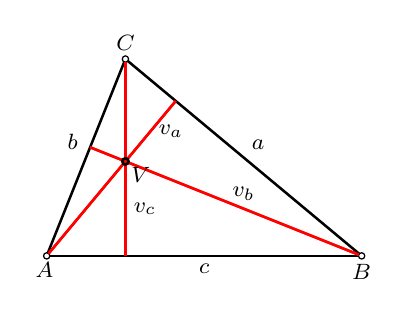
\begin{tikzpicture}
                    % \clip (0,0) rectangle (14.000000,10.000000);
                    {\footnotesize
                    
                    % Marking point A by circle
                    \draw<1-> [line width=0.016cm] (2.000000,1.500000) circle (0.040000);%
                    \draw<1-> (1.970000,1.530000) node [anchor=north] { $A$ };%
                    
                    % Marking point B by circle
                    \draw<1-> [line width=0.016cm] (6.000000,1.500000) circle (0.040000);%
                    \draw<1-> (6.000000,1.500000) node [anchor=north] { $B$ };%
                    
                    % Marking point C by circle
                    \draw<1-> [line width=0.016cm] (3.000000,4.000000) circle (0.040000);%
                    \draw<1-> (3.000000,4.000000) node [anchor=south] { $C$ };%
                    
                    % Marking point c
                    \draw<1-> (4.000000,1.500000) node [anchor=north] { $c$ };%
                    
                    % Marking point a
                    \draw<1-> (4.500000,2.750000) node [anchor=south west] { $a$ };%
                    
                    % Marking point b
                    \draw<1-> (2.500000,2.750000) node [anchor=south east] { $b$ };%
                    
                    % Marking point v_a
                    \draw<2-> (3.319672,3.083607) node [anchor=west] { $v_a$ };%
                    
                    % Marking point v_c
                    \draw<2-> (3.000000,2.100000) node [anchor=west] { $v_c$ };%
                    
                    % Marking point v_b
                    \draw<2-> (4.500000,2.100000) node [anchor=south] { $v_b$ };%
                    
                    % Drawing segment A B
                    \draw<1-> [line width=0.032cm] (2.040000,1.500000) -- (5.960000,1.500000);%
                    
                    % Drawing segment B C
                    \draw<1-> [line width=0.032cm] (5.969271,1.525607) -- (3.030729,3.974393);%
                    
                    % Drawing segment A C
                    \draw<1-> [line width=0.032cm] (2.014856,1.537139) -- (2.985144,3.962861);%
                    
                    % Changing color 255 0 0
                    \definecolor{r255g0b0}{rgb}{1.000000,0.000000,0.000000}%
                    \color{r255g0b0}% 
                    
                    % Drawing segment A A'
                    \draw<2> [line width=0.032cm] (2.025607,1.530729) -- (3.639344,3.467213);%
                    \draw<3-> [line width=0.032cm] (2.025607,1.530729) -- (2.974393,2.669271);%
                    \draw<3-> [line width=0.032cm] (3.025607,2.730729) -- (3.639344,3.467213);%
                    
                    % Drawing segment B B'
                    \draw<2> [line width=0.032cm] (5.962861,1.514856) -- (2.551724,2.879310);%
                    \draw<3-> [line width=0.032cm] (5.962861,1.514856) -- (3.037139,2.685144);%
                    \draw<3-> [line width=0.032cm] (2.962861,2.714856) -- (2.551724,2.879310);%
                    
                    % Drawing segment C C'
                    \draw<2> [line width=0.032cm] (3.000000,3.960000) -- (3.000000,1.500000);%
                    \draw<3-> [line width=0.032cm] (3.000000,3.960000) -- (3.000000,2.740000);%
                    \draw<3-> [line width=0.032cm] (3.000000,2.660000) -- (3.000000,1.500000);%
                    
                    % Changing color 0 0 0
                    \definecolor{r0g0b0}{rgb}{0.000000,0.000000,0.000000}%
                    \color{r0g0b0}% 
                    
                    % Marking point V by circle
                    \draw<3-> [line width=0.032cm] (3.000000,2.700000) circle (0.040000);%
                    \draw<3-> (2.970000,2.730000) node [anchor=north west] { $V$ };%
                    \color{black}
                    }
                \end{tikzpicture}
                    
            \end{figure}

            \onslide<3->{
            \begin{alertblock}{}
                Nosilke vseh treh višin na stranice trikotnika se sekajo v eni točki, ki jo imenujemo \textbf{višinska točka} ali \textbf{ortocenter}.
            \end{alertblock}
            }


            \note{
                TABLA: konstrukcija višin trikotnika z ravnilom in šestilom
                \\
                DOKAZ: Skozi vsako oglišče trikotnika narišemo vzporednico k nasprotni stranici. Presečišča označimo z $A', B', C'$. Zaradi vzporednosti sta štirkotnika $ABA'C$ in $ABCB'$ paralelograma, torej je $|AB|=|A'C|$ in $|AB|=|B'C|$, iz tega $|A'C|=|B'C|$: $C$ razpolavlja $A'B'$. Podobno za $B$ in $A$. Noslike višin trikotnika $ABC$ so simmetrale stranic trikotnika $A'B'C'$. Te se sekajo v središču očrtane krožnice trikotnika $A'B'C'$, ki je višinska točka trikotnika $ABC$.

            }
        \end{frame}


        \begin{frame}

            \begin{alertblock}{}
                \textbf{Težiščnica} na stranico trikotnika je daljica, ki povezuje razpolovišče te stranice z nasprotnim ogliščem. 
            \end{alertblock}

            % \begin{figure}
            %     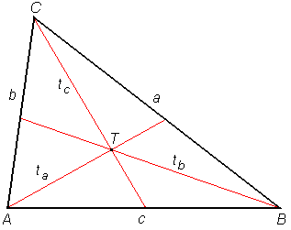
\includegraphics[scale=0.5]{Slike in skice/Teziscnice_in_tezisce.png}
            % \end{figure}

            \begin{figure}
                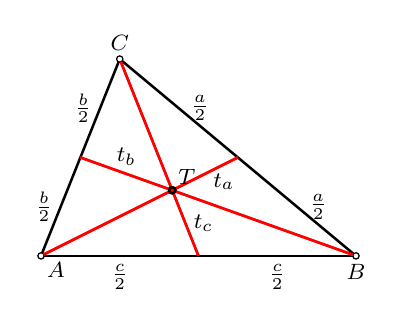
\begin{tikzpicture}
                    % \clip (0,0) rectangle (14.000000,10.000000);
                    {\footnotesize
                    
                    % Marking point A by circle
                    \draw [line width=0.016cm] (2.000000,1.500000) circle (0.040000);%
                    \draw (1.970000,1.530000) node [anchor=north west] { $A$ };%
                    
                    % Marking point B by circle
                    \draw [line width=0.016cm] (6.000000,1.500000) circle (0.040000);%
                    \draw (6.000000,1.500000) node [anchor=north] { $B$ };%
                    
                    % Marking point C by circle
                    \draw [line width=0.016cm] (3.000000,4.000000) circle (0.040000);%
                    \draw (3.000000,4.000000) node [anchor=south] { $C$ };%
                    
                    % Marking point t_a
                    \draw<2-> (4.083333,2.441667) node [anchor=west] { $t_a$ };%
                    
                    % Marking point t_c
                    \draw<2-> (3.833333,1.916667) node [anchor=west] { $t_c$ };%
                    
                    % Marking point t_b
                    \draw<2-> (3.083333,2.541667) node [anchor=south] { $t_b$ };%
                    
                    % Marking point \frac{b}{2}
                    \draw<2-> (2.250000,2.125000) node [anchor=east] { $\frac{b}{2}$ };%
                    
                    % Marking point \frac{b}{2}
                    \draw<2-> (2.750000,3.375000) node [anchor=east] { $\frac{b}{2}$ };%
                    
                    % Marking point \frac{c}{2}
                    \draw<2-> (3.000000,1.500000) node [anchor=north] { $\frac{c}{2}$ };%
                    
                    % Marking point \frac{c}{2}
                    \draw<2-> (5.000000,1.500000) node [anchor=north] { $\frac{c}{2}$ };%
                    
                    % Marking point \frac{a}{2}
                    \draw<2-> (5.30000,2.125000) node [anchor=west] { $\frac{a}{2}$ };%
                    
                    % Marking point \frac{a}{2}
                    \draw<2-> (3.80000,3.375000) node [anchor=west] { $\frac{a}{2}$ };%
                    
                    % Drawing segment A B
                    \draw [line width=0.032cm] (2.040000,1.500000) -- (5.960000,1.500000);%
                    
                    % Drawing segment B C
                    \draw [line width=0.032cm] (5.969271,1.525607) -- (3.030729,3.974393);%
                    
                    % Drawing segment A C
                    \draw [line width=0.032cm] (2.014856,1.537139) -- (2.985144,3.962861);%
                    
                    % Changing color 255 0 0
                    \definecolor{r255g0b0}{rgb}{1.000000,0.000000,0.000000}%
                    \color{r255g0b0}% 
                    
                    % Drawing segment A a
                    \draw<2> [line width=0.032cm] (2.035777,1.517889) -- (4.500000,2.750000);%
                    \draw<3-> [line width=0.032cm] (2.035777,1.517889) -- (3.630890,2.315445);%
                    \draw<3-> [line width=0.032cm] (3.702444,2.351222) -- (4.500000,2.750000);%
                    
                    % Drawing segment B b
                    \draw<2> [line width=0.032cm] (5.962330,1.513453) -- (2.500000,2.750000);%
                    \draw<3-> [line width=0.032cm] (5.962330,1.513453) -- (3.704336,2.319880);%
                    \draw<3-> [line width=0.032cm] (3.628997,2.346787) -- (2.500000,2.750000);%
                    
                    % Drawing segment C c
                    \draw<2> [line width=0.032cm] (3.014856,3.962861) -- (4.000000,1.500000);%
                    \draw<3-> [line width=0.032cm] (3.014856,3.962861) -- (3.651811,2.370472);%
                    \draw<3-> [line width=0.032cm] (3.681522,2.296194) -- (4.000000,1.500000);%
                    
                    % Changing color 0 0 0
                    \definecolor{r0g0b0}{rgb}{0.000000,0.000000,0.000000}%
                    \color{r0g0b0}% 
                    
                    % Marking point T by circle
                    \draw<3-> [line width=0.032cm] (3.666667,2.333333) circle (0.040000);%
                    \draw<3-> (3.636667,2.303333) node [anchor=south west] { $T$ };%
                    \color{black}
                    }
                \end{tikzpicture}
                    
            \end{figure}

            \onslide<3->{
            \begin{alertblock}{}
                Vse tri trikotnikove težiščnice se sekajo v eni točki -- \textbf{težišču} ali \textbf{baricentru} trikotnika. \\ 
                Težišče deli težiščnico v razmerju $1:2$.
            \end{alertblock}
            }

            \note{
                TABLA: konstrukcija težišnic z ravnilom in šestilom
            }

        \end{frame}


        % \begin{frame}
        %     \begin{exampleblock}{Naloga 81}
        %         Konstruiraj trikotnik.
        %         \begin{itemize}
        %             \item $a=2~cm,\ b=6~cm,\ c=5~cm$;
        %             \item $c=4~cm,\ \alpha=60^\circ,\ \beta=45^\circ$;
        %             \item $a=4~cm,\ c=5~cm,\ \alpha=45^\circ$;
        %             \item $a=2,5~cm,\ c=5~cm,\ v_c=2~cm$;
        %             \item $v_c=3~cm,\ \alpha=60^\circ,\ \beta=75^\circ$;
        %             \item $v_a=2~cm,\ v_b=4~cm,\ \gamma=45^\circ$;
        %             \item $b=65~cm,\ t_b=3,5~cm,\ \gamma=60^\circ$;
        %             \item $v_a=3~cm,\ t_c=4~cm,\ \beta=45^\circ$.
        %         \end{itemize}
        %     \end{exampleblock}


        %     \note{
        %         Morda manj primerov pri nalogi 81. (b, c, h, l, n, r, š, u)
        %     }
        % \end{frame}


        \begin{frame}

            \begin{alertblock}{}
                Simetrale vseh treh stranic trikotnika se sekajo v eni točki. Ta točka je \textbf{središče trikotniku očrtane krožnice}. 
            \end{alertblock}

            % \begin{figure}
            %     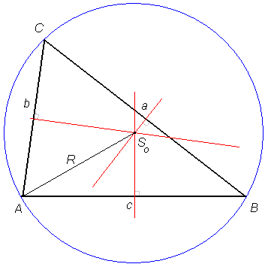
\includegraphics[scale=0.55]{Slike in skice/Trikotniku_ocrtana_kroznica.png}
            % \end{figure}

            \begin{figure}
                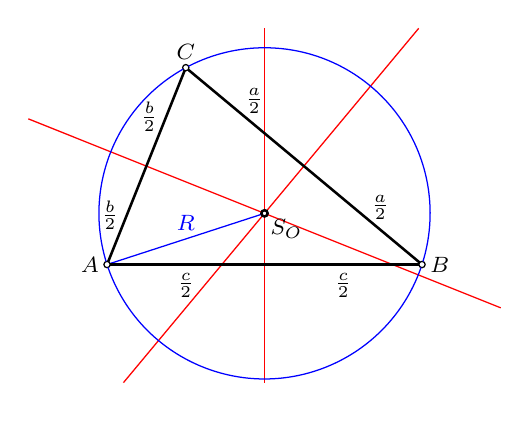
\begin{tikzpicture}
                    % \clip (0,0) rectangle (14.000000,10.000000);
                    {\footnotesize
                    
                    % Marking point A by circle
                    \draw [line width=0.016cm] (2.000000,2.500000) circle (0.040000);%
                    \draw (2.000000,2.500000) node [anchor=east] { $A$ };%
                    
                    % Marking point B by circle
                    \draw [line width=0.016cm] (6.000000,2.500000) circle (0.040000);%
                    \draw (6.000000,2.500000) node [anchor=west] { $B$ };%
                    
                    % Marking point C by circle
                    \draw [line width=0.016cm] (3.000000,5.000000) circle (0.040000);%
                    \draw (3.000000,5.000000) node [anchor=south] { $C$ };%
                    
                    % Marking point \frac{b}{2}
                    \draw (2.250000,3.125000) node [anchor=east] { $\frac{b}{2}$ };%
                    
                    % Marking point \frac{b}{2}
                    \draw (2.750000,4.375000) node [anchor=east] { $\frac{b}{2}$ };%
                    
                    % Marking point \frac{c}{2}
                    \draw (3.000000,2.500000) node [anchor=north] { $\frac{c}{2}$ };%
                    
                    % Marking point \frac{c}{2}
                    \draw (5.000000,2.500000) node [anchor=north] { $\frac{c}{2}$ };%
                    
                    % Marking point \frac{a}{2}
                    \draw (5.250000,3.225000) node [anchor=west] { $\frac{a}{2}$ };%
                    
                    % Marking point \frac{a}{2}
                    \draw (3.650000,4.575000) node [anchor=west] { $\frac{a}{2}$ };%
                    
                    % Changing color 255 0 0
                    \definecolor{r255g0b0}{rgb}{1.000000,0.000000,0.000000}%
                    \color{r255g0b0}% 
                    
                    % Drawing line s_c
                    \draw [line width=0.016cm] (4.000000,1.000000) -- (4.000000,3.110000);%
                    \draw [line width=0.016cm] (4.000000,3.190000) -- (4.000000,5.500000);%
                    
                    % Drawing line s_a
                    \draw [line width=0.016cm] (2.208333,1.000000) -- (3.974393,3.119271);%
                    \draw [line width=0.016cm] (4.025607,3.180729) -- (5.958333,5.500000);%
                    
                    % Drawing line s_b
                    \draw [line width=0.016cm] (1.000000,4.350000) -- (3.962861,3.164856);%
                    \draw [line width=0.016cm] (4.037139,3.135144) -- (7.000000,1.950000);%
                    
                    % Changing color 0 0 255
                    \definecolor{r0g0b255}{rgb}{0.000000,0.000000,1.000000}%
                    \color{r0g0b255}% 
                    
                    % Drawing circle S_O A
                    \draw [line width=0.016cm] (2.012724,2.462079) -- (2.023851,2.430741) arc (200:340:2.102974 and 2.102974) -- (5.987275,2.462077);%
                    \draw [line width=0.016cm] (6.012001,2.538157) -- (6.021508,2.570341) arc (344:360:2.102974 and 2.102974) --(6.102974,3.150000) arc (0:117:2.102974 and 2.102974) -- (3.035368,5.018685);%
                    \draw [line width=0.016cm] (2.964994,4.980646) -- (2.948513,4.971229) arc (120:196:2.102974 and 2.102974) -- (1.987999,2.538158);%
                    
                    % Drawing segment A S_O
                    \draw [line width=0.016cm] (2.038041,2.512363) -- (3.961959,3.137637);%
                    
                    % Marking point R
                    \draw (3.000000,2.825000) node [anchor=south] { $R$ };%
                    
                    % Changing color 0 0 0
                    \definecolor{r0g0b0}{rgb}{0.000000,0.000000,0.000000}%
                    \color{r0g0b0}% 
                    
                    % Drawing segment A B
                    \draw [line width=0.032cm] (2.040000,2.500000) -- (5.960000,2.500000);%
                    
                    % Drawing segment B C
                    \draw [line width=0.032cm] (5.969271,2.525607) -- (3.030729,4.974393);%
                    
                    % Drawing segment A C
                    \draw [line width=0.032cm] (2.014856,2.537139) -- (2.985144,4.962861);%
                    
                    % Marking point S_O by circle
                    \draw [line width=0.032cm] (4.000000,3.150000) circle (0.040000);%
                    \draw (3.970000,3.180000) node [anchor=north west] { $S_O$ };%
                    \color{black}
                    }
                \end{tikzpicture}    

            \end{figure}

            \pause
            Očrtana krožnica poteka skozi vsa tri oglišča trikotnika. Vse tri stranice trikotnika so tetive te krožnice.


            \note{
                TABLA: konstrukcija simetral stranic in očrtane krožnice z ravnilom in šestilom
                \\
                DOKAZ: Konstruiramo simetrali stranic $AC$ in $AB$. Vsaka točka na njiju je enako oddaljena od oglišč stranice. Torej je njuno presečišče $S_O$ enako oddalje od vseh trh oglišč $A, B, C$ in tako središče trikotniku očrtane krožnice. Podbno za simetralo strannice $BC$.
            }
        \end{frame}


        \begin{frame}

            \begin{alertblock}{}
                Simetrale notranjih kotov trikotnika se sekajo v eni točki. Ta točka je \textbf{središče trikotniku včrtane krožnice}.
            \end{alertblock}

            % \begin{figure}
            %     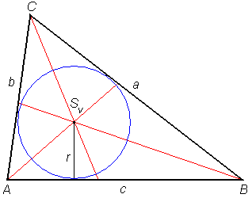
\includegraphics[scale=0.65]{Slike in skice/Trikotniku_vcrtana_kroznica.png}
            % \end{figure}

            \begin{figure}
                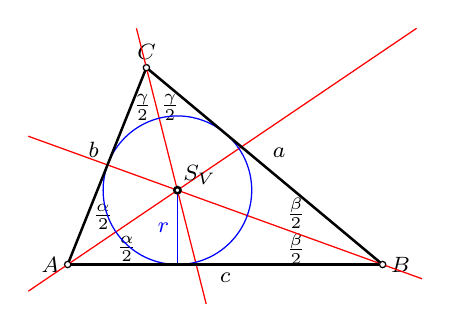
\begin{tikzpicture}
                    % \clip (0,0) rectangle (14.000000,10.000000);
                    {\footnotesize
                    
                    % Marking point A by circle
                    \draw [line width=0.016cm] (2.000000,2.500000) circle (0.040000);%
                    \draw (2.000000,2.500000) node [anchor=east] { $A$ };%
                    
                    % Marking point B by circle
                    \draw [line width=0.016cm] (6.000000,2.500000) circle (0.040000);%
                    \draw (6.000000,2.500000) node [anchor=west] { $B$ };%
                    
                    % Marking point C by circle
                    \draw [line width=0.016cm] (3.000000,5.000000) circle (0.040000);%
                    \draw (3.000000,5.000000) node [anchor=south] { $C$ };%
                    
                    % Marking point b
                    \draw (2.500000,3.750000) node [anchor=south east] { $b$ };%
                    
                    % Marking point c
                    \draw (4.000000,2.500000) node [anchor=north] { $c$ };%
                    
                    % Marking point a
                    \draw (4.500000,3.750000) node [anchor=south west] { $a$ };%
                    
                    % Marking point \frac{\alpha}{2}
                    \draw (2.750000,2.700000) node  { $\frac{\alpha}{2}$ };%
                    
                    % Marking point \frac{\gamma}{2}
                    \draw (2.950000,4.500000) node  { $\frac{\gamma}{2}$ };%
                    
                    % Marking point \frac{\alpha}{2}
                    \draw (2.450000,3.100000) node  { $\frac{\alpha}{2}$ };%
                    
                    % Marking point \frac{\beta}{2}
                    \draw (4.900000,2.700000) node  { $\frac{\beta}{2}$ };%
                    
                    % Marking point \frac{\beta}{2}
                    \draw (4.900000,3.150000) node  { $\frac{\beta}{2}$ };%
                    
                    % Marking point \frac{\gamma}{2}
                    \draw (3.300000,4.500000) node  { $\frac{\gamma}{2}$ };%
                    
                    % Changing color 255 0 0
                    \definecolor{r255g0b0}{rgb}{1.000000,0.000000,0.000000}%
                    \color{r255g0b0}% 
                    
                    % Drawing line s_c
                    \draw [line width=0.016cm] (3.758922,2.000000) -- (3.403539,3.404822);%
                    \draw [line width=0.016cm] (3.383919,3.482379) -- (3.009810,4.961222);%
                    \draw [line width=0.016cm] (2.990190,5.038778) -- (2.873513,5.500000);%
                    
                    % Drawing line s_a
                    \draw [line width=0.016cm] (6.431099,5.500000) -- (3.426851,3.466025);%
                    \draw [line width=0.016cm] (3.360606,3.421175) -- (2.033123,2.522425);%
                    \draw [line width=0.016cm] (1.966877,2.477575) -- (1.500000,2.161484);%
                    
                    % Drawing line s_b
                    \draw [line width=0.016cm] (1.500000,4.129225) -- (3.356118,3.457217);%
                    \draw [line width=0.016cm] (3.431340,3.429983) -- (5.962389,2.513617);%
                    \draw [line width=0.016cm] (6.037611,2.486383) -- (6.500000,2.318975);%
                    
                    % Changing color 0 0 255
                    \definecolor{r0g0b255}{rgb}{0.000000,0.000000,1.000000}%
                    \color{r0g0b255}% 
                    
                    % Drawing circle S_V X
                    \draw [line width=0.016cm] (3.393729,3.443600) circle (0.943600);%
                    
                    % Drawing segment X S_V
                    \draw [line width=0.016cm] (3.393729,2.500000) -- (3.393729,3.403600);%
                    
                    % Marking point r
                    \draw (3.393729,2.971800) node [anchor=east] { $r$ };%
                    
                    % Changing color 0 0 0
                    \definecolor{r0g0b0}{rgb}{0.000000,0.000000,0.000000}%
                    \color{r0g0b0}% 
                    
                    % Drawing segment A B
                    \draw [line width=0.032cm] (2.040000,2.500000) -- (5.960000,2.500000);%
                    
                    % Drawing segment B C
                    \draw [line width=0.032cm] (5.969271,2.525607) -- (3.030729,4.974393);%
                    
                    % Drawing segment A C
                    \draw [line width=0.032cm] (2.014856,2.537139) -- (2.985144,4.962861);%
                    
                    % Marking point S_V by circle
                    \draw [line width=0.032cm] (3.393729,3.443600) circle (0.040000);%
                    \draw (3.363729,3.413600) node [anchor=south west] { $S_V$ };%
                    \color{black}
                    }
                \end{tikzpicture}
                    
            \end{figure}
            
            \pause
            Včrtana krožnica ima vse tri stranice trikotnika za tangente.


            \note{
                TABLA: konstrukcija simetral kotov in včrtane krožnice z ravnilom in šestilom
                \\
                DOKAZ: Narišemo simetrali kotov pri $A$ in $B$. Vsaka točka na njiju je enako oddaljena od nosilk stranic ob kotu. Njuno presečišče $S_V$ je torej enako oddalje od vseh treh nosilk stranic trikotnika. In zatorej je središče krožnice, ki se dotika vseh treh stranic -- trikotniku včrtane krožnice.
            }
        \end{frame}

        % \begin{frame}
        %     \begin{exampleblock}{Naloga 83}
        %         Dan je trikotnik $\triangle ABC$ s podatki $b=5~cm,\ \beta=45^\circ,\ \gamma=60^\circ$.
        %         \begin{enumerate}
        %             \item Konstruiraj trikotnik $\triangle ABC$.
        %             \item Konstruiraj trikotniku $\triangle ABC$ očrtano krožnico.
        %             \item Koliko je velik zunanji kot pri oglišču $A$?
        %         \end{enumerate}
        %     \end{exampleblock}

        %     \pause
        %     \begin{exampleblock}{Naloga 84}
        %         Dan je trikotnik $\triangle ABC$ s podatki $a=5~cm,\ c=4~cm,\ t_c=4~cm$.
        %         \begin{enumerate}
        %             \item Konstruiraj trikotnik $\triangle ABC$.
        %             \item Konstruiraj trikotniku $\triangle ABC$ včrtano krožnico.
        %             \item Kateri izmed $\angle BAC$ in $\angle ACB$ je večji? Utemelji (brez merjenja).
        %         \end{enumerate}
        %     \end{exampleblock}
        % \end{frame}


        \begin{frame}

            \begin{alertblock}{}
                Težišče, središče trikotniku očrtane kroznice, središče trikotniku včrtane krožnice in višinska točka so \textbf{znamenite točke trikotnika}.

            \end{alertblock}

            \pause
            \begin{alertblock}{}
                Višinska točka, središče očrtane krožnice in težišče so vedno kolinearne. Premico, ki jih povezuje, imenujemo \textbf{Eulerjeva premica}.
            \end{alertblock}

            % \begin{figure}
            %     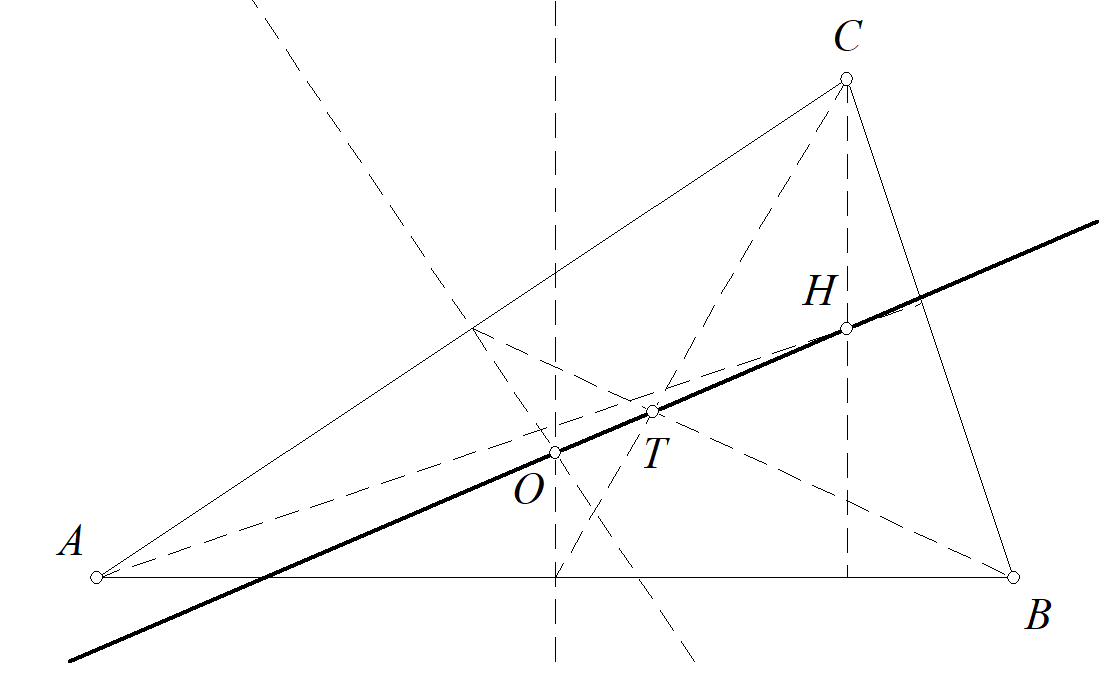
\includegraphics[scale=0.23]{Slike in skice/Eulerjeva_premica.png}
            % \end{figure}

            \begin{figure}
                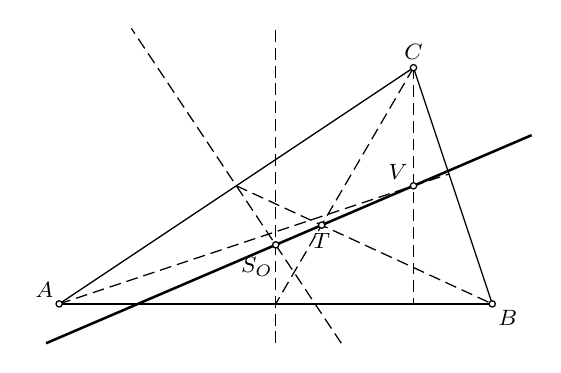
\begin{tikzpicture}
                    % \clip (0,0) rectangle (14.000000,10.000000);
                    {\footnotesize
                    
                    % Drawing segment A B
                    \draw [line width=0.016cm] (1.540000,3.500000) -- (6.960000,3.500000);%
                    
                    % Drawing segment A C
                    \draw [line width=0.016cm] (1.533282,3.522188) -- (5.966718,6.477812);%
                    
                    % Drawing segment B C
                    \draw [line width=0.016cm] (6.987351,3.537947) -- (6.012649,6.462053);%
                    
                    % Drawing line b
                    \draw [line width=0.016cm] (5.083333,3.000000) -- (5.000128,3.124808);%
                    \draw [line width=0.016cm] (4.958526,3.187211) -- (4.875321,3.312019);%
                    \draw [line width=0.016cm] (4.833718,3.374423) -- (4.750513,3.499230);%
                    \draw [line width=0.016cm] (4.708911,3.561634) -- (4.625706,3.686441);%
                    \draw [line width=0.016cm] (4.584103,3.748845) -- (4.500898,3.873653);%
                    \draw [line width=0.016cm] (4.459296,3.936057) -- (4.376091,4.060864);%
                    \draw [line width=0.016cm] (4.334488,4.123268) -- (4.272188,4.216718);%
                    \draw [line width=0.016cm] (4.209681,4.310479) -- (4.126475,4.435287);%
                    \draw [line width=0.016cm] (4.084873,4.497691) -- (4.001668,4.622498);%
                    \draw [line width=0.016cm] (3.960065,4.684902) -- (3.876860,4.809709);%
                    \draw [line width=0.016cm] (3.835258,4.872113) -- (3.752053,4.996921);%
                    \draw [line width=0.016cm] (3.710450,5.059324) -- (3.627245,5.184132);%
                    \draw [line width=0.016cm] (3.585643,5.246536) -- (3.502438,5.371343);%
                    \draw [line width=0.016cm] (3.460835,5.433747) -- (3.377630,5.558555);%
                    \draw [line width=0.016cm] (3.336028,5.620958) -- (3.252823,5.745766);%
                    \draw [line width=0.016cm] (3.211220,5.808170) -- (3.128015,5.932977);%
                    \draw [line width=0.016cm] (3.086413,5.995381) -- (3.003208,6.120189);%
                    \draw [line width=0.016cm] (2.961605,6.182592) -- (2.878400,6.307400);%
                    \draw [line width=0.016cm] (2.836798,6.369804) -- (2.753593,6.494611);%
                    \draw [line width=0.016cm] (2.711990,6.557015) -- (2.628785,6.681823);%
                    \draw [line width=0.016cm] (2.587182,6.744226) -- (2.503977,6.869034);%
                    \draw [line width=0.016cm] (2.462375,6.931438) -- (2.416667,7.000000);%
                    
                    % Drawing line c
                    \draw [line width=0.016cm] (4.250000,3.000000) -- (4.250000,3.150000);%
                    \draw [line width=0.016cm] (4.250000,3.225000) -- (4.250000,3.375000);%
                    \draw [line width=0.016cm] (4.250000,3.450000) -- (4.250000,3.600000);%
                    \draw [line width=0.016cm] (4.250000,3.675000) -- (4.250000,3.825000);%
                    \draw [line width=0.016cm] (4.250000,3.900000) -- (4.250000,4.050000);%
                    \draw [line width=0.016cm] (4.250000,4.125000) -- (4.250000,4.210000);%
                    \draw [line width=0.016cm] (4.250000,4.350000) -- (4.250000,4.500000);%
                    \draw [line width=0.016cm] (4.250000,4.575000) -- (4.250000,4.725000);%
                    \draw [line width=0.016cm] (4.250000,4.800000) -- (4.250000,4.950000);%
                    \draw [line width=0.016cm] (4.250000,5.025000) -- (4.250000,5.175000);%
                    \draw [line width=0.016cm] (4.250000,5.250000) -- (4.250000,5.400000);%
                    \draw [line width=0.016cm] (4.250000,5.475000) -- (4.250000,5.625000);%
                    \draw [line width=0.016cm] (4.250000,5.700000) -- (4.250000,5.850000);%
                    \draw [line width=0.016cm] (4.250000,5.925000) -- (4.250000,6.075000);%
                    \draw [line width=0.016cm] (4.250000,6.150000) -- (4.250000,6.300000);%
                    \draw [line width=0.016cm] (4.250000,6.375000) -- (4.250000,6.525000);%
                    \draw [line width=0.016cm] (4.250000,6.600000) -- (4.250000,6.750000);%
                    \draw [line width=0.016cm] (4.250000,6.825000) -- (4.250000,6.975000);%
                    
                    % Drawing segment C C'
                    \draw [line width=0.016cm] (5.979845,6.465449) -- (5.924419,6.370433);%
                    \draw [line width=0.016cm] (5.886629,6.305650) -- (5.811048,6.176083);%
                    \draw [line width=0.016cm] (5.773258,6.111299) -- (5.697677,5.981733);%
                    \draw [line width=0.016cm] (5.659887,5.916949) -- (5.584306,5.787382);%
                    \draw [line width=0.016cm] (5.546516,5.722599) -- (5.470935,5.593032);%
                    \draw [line width=0.016cm] (5.433145,5.528249) -- (5.357564,5.398682);%
                    \draw [line width=0.016cm] (5.319774,5.333898) -- (5.244193,5.204332);%
                    \draw [line width=0.016cm] (5.206403,5.139548) -- (5.130822,5.009981);%
                    \draw [line width=0.016cm] (5.093032,4.945198) -- (5.017452,4.815631);%
                    \draw [line width=0.016cm] (4.979661,4.750848) -- (4.904081,4.621281);%
                    \draw [line width=0.016cm] (4.866290,4.556497) -- (4.853488,4.534551);%
                    \draw [line width=0.016cm] (4.813178,4.465449) -- (4.790710,4.426931);%
                    \draw [line width=0.016cm] (4.752919,4.362147) -- (4.677339,4.232580);%
                    \draw [line width=0.016cm] (4.639548,4.167797) -- (4.563968,4.038230);%
                    \draw [line width=0.016cm] (4.526177,3.973447) -- (4.450597,3.843880);%
                    \draw [line width=0.016cm] (4.412806,3.779096) -- (4.337226,3.649530);%
                    \draw [line width=0.016cm] (4.299435,3.584746) -- (4.250000,3.500000);%
                    
                    % Drawing segment C U
                    \draw [line width=0.016cm] (6.000000,6.460000) -- (6.000000,6.350000);%
                    \draw [line width=0.016cm] (6.000000,6.275000) -- (6.000000,6.125000);%
                    \draw [line width=0.016cm] (6.000000,6.050000) -- (6.000000,5.900000);%
                    \draw [line width=0.016cm] (6.000000,5.825000) -- (6.000000,5.675000);%
                    \draw [line width=0.016cm] (6.000000,5.600000) -- (6.000000,5.450000);%
                    \draw [line width=0.016cm] (6.000000,5.375000) -- (6.000000,5.225000);%
                    \draw [line width=0.016cm] (6.000000,5.150000) -- (6.000000,5.040000);%
                    \draw [line width=0.016cm] (6.000000,4.925000) -- (6.000000,4.775000);%
                    \draw [line width=0.016cm] (6.000000,4.700000) -- (6.000000,4.550000);%
                    \draw [line width=0.016cm] (6.000000,4.475000) -- (6.000000,4.325000);%
                    \draw [line width=0.016cm] (6.000000,4.250000) -- (6.000000,4.100000);%
                    \draw [line width=0.016cm] (6.000000,4.025000) -- (6.000000,3.875000);%
                    \draw [line width=0.016cm] (6.000000,3.800000) -- (6.000000,3.650000);%
                    \draw [line width=0.016cm] (6.000000,3.575000) -- (6.000000,3.500000);%
                    
                    % Drawing segment A V
                    \draw [line width=0.016cm] (1.537947,3.512649) -- (1.642302,3.547434);%
                    \draw [line width=0.016cm] (1.713454,3.571151) -- (1.855756,3.618585);%
                    \draw [line width=0.016cm] (1.926907,3.642302) -- (2.069210,3.689737);%
                    \draw [line width=0.016cm] (2.140361,3.713454) -- (2.282664,3.760888);%
                    \draw [line width=0.016cm] (2.353815,3.784605) -- (2.496117,3.832039);%
                    \draw [line width=0.016cm] (2.567269,3.855756) -- (2.709571,3.903190);%
                    \draw [line width=0.016cm] (2.780722,3.926907) -- (2.923025,3.974342);%
                    \draw [line width=0.016cm] (2.994176,3.998059) -- (3.136479,4.045493);%
                    \draw [line width=0.016cm] (3.207630,4.069210) -- (3.349932,4.116644);%
                    \draw [line width=0.016cm] (3.421084,4.140361) -- (3.563386,4.187795);%
                    \draw [line width=0.016cm] (3.634537,4.211512) -- (3.776840,4.258947);%
                    \draw [line width=0.016cm] (3.847991,4.282664) -- (3.990294,4.330098);%
                    \draw [line width=0.016cm] (4.061445,4.353815) -- (4.203747,4.401249);%
                    \draw [line width=0.016cm] (4.274899,4.424966) -- (4.417201,4.472400);%
                    \draw [line width=0.016cm] (4.488352,4.496117) -- (4.630655,4.543552);%
                    \draw [line width=0.016cm] (4.701806,4.567269) -- (4.844109,4.614703);%
                    \draw [line width=0.016cm] (4.915260,4.638420) -- (5.057562,4.685854);%
                    \draw [line width=0.016cm] (5.128714,4.709571) -- (5.271016,4.757005);%
                    \draw [line width=0.016cm] (5.342167,4.780722) -- (5.484470,4.828157);%
                    \draw [line width=0.016cm] (5.555621,4.851874) -- (5.697924,4.899308);%
                    \draw [line width=0.016cm] (5.769075,4.923025) -- (5.911377,4.970459);%
                    \draw [line width=0.016cm] (6.037947,5.012649) -- (6.124831,5.041610);%
                    \draw [line width=0.016cm] (6.195982,5.065327) -- (6.338285,5.112762);%
                    \draw [line width=0.016cm] (6.409436,5.136479) -- (6.450000,5.150000);%
                    
                    % Drawing segment B' B
                    \draw [line width=0.016cm] (3.750000,5.000000) -- (3.886194,4.937141);%
                    \draw [line width=0.016cm] (3.954291,4.905712) -- (4.090485,4.842853);%
                    \draw [line width=0.016cm] (4.158582,4.811424) -- (4.294776,4.748565);%
                    \draw [line width=0.016cm] (4.362873,4.717136) -- (4.499066,4.654277);%
                    \draw [line width=0.016cm] (4.567163,4.622848) -- (4.703357,4.559989);%
                    \draw [line width=0.016cm] (4.771454,4.528560) -- (4.797015,4.516762);%
                    \draw [line width=0.016cm] (4.869652,4.483238) -- (4.907648,4.465701);%
                    \draw [line width=0.016cm] (4.975745,4.434271) -- (5.111939,4.371413);%
                    \draw [line width=0.016cm] (5.180036,4.339983) -- (5.316230,4.277125);%
                    \draw [line width=0.016cm] (5.384327,4.245695) -- (5.520521,4.182837);%
                    \draw [line width=0.016cm] (5.588618,4.151407) -- (5.724812,4.088548);%
                    \draw [line width=0.016cm] (5.792909,4.057119) -- (5.929103,3.994260);%
                    \draw [line width=0.016cm] (5.997199,3.962831) -- (6.133393,3.899972);%
                    \draw [line width=0.016cm] (6.201490,3.868543) -- (6.337684,3.805684);%
                    \draw [line width=0.016cm] (6.405781,3.774255) -- (6.541975,3.711396);%
                    \draw [line width=0.016cm] (6.610072,3.679967) -- (6.746266,3.617108);%
                    \draw [line width=0.016cm] (6.814363,3.585679) -- (6.950557,3.522820);%
                    
                    % Marking point A by circle
                    \draw [line width=0.016cm] (1.500000,3.500000) circle (0.040000);%
                    \draw (1.530000,3.470000) node [anchor=south east] { $A$ };%
                    
                    % Marking point B by circle
                    \draw [line width=0.016cm] (7.000000,3.500000) circle (0.040000);%
                    \draw (6.970000,3.530000) node [anchor=north west] { $B$ };%
                    
                    % Marking point C by circle
                    \draw [line width=0.016cm] (6.000000,6.500000) circle (0.040000);%
                    \draw (6.000000,6.500000) node [anchor=south] { $C$ };%
                    
                    % Marking point O by circle
                    \draw [line width=0.016cm] (4.250000,4.250000) circle (0.040000);%
                    \draw (4.320000,4.200000) node [anchor=north east] { $S_O$ };%
                    
                    % Marking point T by circle
                    \draw [line width=0.016cm] (4.833333,4.500000) circle (0.040000);%
                    \draw (4.833333,4.500000) node [anchor=north] { $T$ };%
                    
                    % Marking point H_C by circle
                    \draw [line width=0.016cm] (6.000000,5.000000) circle (0.040000);%
                    \draw (6.030000,4.970000) node [anchor=south east] { $V$ };%
                    
                    % Drawing line O T
                    \draw [line width=0.032cm] (1.333333,3.000000) -- (4.213234,4.234243);%
                    \draw [line width=0.032cm] (4.286766,4.265757) -- (4.796568,4.484243);%
                    \draw [line width=0.032cm] (4.870099,4.515757) -- (5.963234,4.984243);%
                    \draw [line width=0.032cm] (6.036766,5.015757) -- (7.500000,5.642857);%
                    }
                \end{tikzpicture}
                    
            \end{figure}
            

        \end{frame}

        \begin{frame}
            \large\textbf{Vrste trikotnikov -- glede na stranice}
            % ~\\
            \normalsize
            \begin{columns}
                \column<2->{0.35\textwidth}
                \begin{exampleblock}{}
                    RAZNOSTRANIČNI TRIKOTNIK 

                    \begin{figure}
                        \begin{tikzpicture}
                            % \clip (0,0) rectangle (14.000000,10.000000);
                            {\footnotesize
                            
                            % Marking point A by circle
                            \draw [line width=0.016cm] (1.500000,1.500000) circle (0.040000);%
                            \draw (1.500000,1.500000) node [anchor=north] { $A$ };%
                            
                            % Marking point B by circle
                            \draw [line width=0.016cm] (6.000000,1.500000) circle (0.040000);%
                            \draw (6.000000,1.500000) node [anchor=north] { $B$ };%
                            
                            % Marking point C by circle
                            \draw [line width=0.016cm] (4.500000,4.500000) circle (0.040000);%
                            \draw (4.500000,4.500000) node [anchor=south] { $C$ };%
                            
                            % Changing color 255 0 0
                            \definecolor{r255g0b0}{rgb}{1.000000,0.000000,0.000000}%
                            \color{r255g0b0}% 
                            
                            % Drawing segment B C
                            \draw [line width=0.016cm] (5.982111,1.535777) -- (4.517889,4.464223);%
                            
                            % Marking point a
                            \draw (5.250000,3.000000) node [anchor=south west] { $a$ };%
                            
                            % Changing color 0 255 0
                            \definecolor{r0g255b0}{rgb}{0.000000,1.000000,0.000000}%
                            \color{r0g255b0}% 
                            
                            % Drawing segment A C
                            \draw [line width=0.016cm] (1.528284,1.528284) -- (4.471716,4.471716);%
                            
                            % Marking point b
                            \draw (3.000000,3.000000) node [anchor=south east] { $b$ };%
                            
                            % Changing color 0 0 255
                            \definecolor{r0g0b255}{rgb}{0.000000,0.000000,1.000000}%
                            \color{r0g0b255}% 
                            
                            % Drawing segment A B
                            \draw [line width=0.016cm] (1.540000,1.500000) -- (5.960000,1.500000);%
                            
                            % Marking point c
                            \draw (3.750000,1.500000) node [anchor=north] { $c$ };%
                            \color{black}
                            }
                        \end{tikzpicture}
                            
                    \end{figure}

                    vse tri stranice različno dolge 
                    % $\Rightarrow$ vsi trije koti so različni
                    
                \end{exampleblock}
                \column<3->{0.27\textwidth}
                \begin{exampleblock}{}
                    ENAKOKRAKI TRIKOTNIK 

                    \begin{figure}
                        \begin{tikzpicture}
                            % \clip (0,0) rectangle (14.000000,10.000000);
                            {\footnotesize
                            
                            % Marking point A by circle
                            \draw [line width=0.016cm] (1.500000,1.500000) circle (0.040000);%
                            \draw (1.500000,1.500000) node [anchor=north] { $A$ };%
                            
                            % Marking point B by circle
                            \draw [line width=0.016cm] (5.000000,1.500000) circle (0.040000);%
                            \draw (5.000000,1.500000) node [anchor=north] { $B$ };%
                            
                            % Marking point C by circle
                            \draw [line width=0.016cm] (3.250000,5.000000) circle (0.040000);%
                            \draw (3.250000,5.000000) node [anchor=south] { $C$ };%
                            
                            % Changing color 255 0 0
                            \definecolor{r255g0b0}{rgb}{1.000000,0.000000,0.000000}%
                            \color{r255g0b0}% 
                            
                            % Drawing segment B C
                            \draw [line width=0.016cm] (4.982111,1.535777) -- (3.267889,4.964223);%
                            
                            % Marking point a
                            \draw (4.125000,3.250000) node [anchor=south west] { $a$ };%
                            
                            % Drawing segment A C
                            \draw [line width=0.016cm] (1.517889,1.535777) -- (3.232111,4.964223);%
                            
                            % Marking point a
                            \draw (2.375000,3.250000) node [anchor=south east] { $a$ };%
                            
                            % Changing color 0 0 255
                            \definecolor{r0g0b255}{rgb}{0.000000,0.000000,1.000000}%
                            \color{r0g0b255}% 
                            
                            % Drawing segment A B
                            \draw [line width=0.016cm] (1.540000,1.500000) -- (4.960000,1.500000);%
                            
                            % Marking point c
                            \draw (3.250000,1.500000) node [anchor=north] { $c$ };%
                            \color{black}
                            }
                        \end{tikzpicture}
                            
                    \end{figure}

                    dve stranici enako dolgi 
                    % $\Rightarrow$ kota ob osnovnici sta skladna
                    
                \end{exampleblock}                
                \column<4->{0.31\textwidth}
                \begin{exampleblock}{}
                    ENAKOSTRANIČNI ali PRAVILNI TRIKOTNIK 

                    \begin{figure}
                        \begin{tikzpicture}
                            % \clip (0,0) rectangle (14.000000,10.000000);
                            {\footnotesize
                            
                            % Marking point A by circle
                            \draw [line width=0.016cm] (1.500000,1.500000) circle (0.040000);%
                            \draw (1.500000,1.500000) node [anchor=north] { $A$ };%
                            
                            % Marking point B by circle
                            \draw [line width=0.016cm] (5.500000,1.500000) circle (0.040000);%
                            \draw (5.500000,1.500000) node [anchor=north] { $B$ };%
                            
                            % Marking point C by circle
                            \draw [line width=0.016cm] (3.500000,5.000000) circle (0.040000);%
                            \draw (3.500000,5.000000) node [anchor=south] { $C$ };%
                            
                            % Changing color 0 255 0
                            \definecolor{r0g255b0}{rgb}{0.000000,1.000000,0.000000}%
                            \color{r0g255b0}% 
                            
                            % Drawing segment B C
                            \draw [line width=0.016cm] (5.480154,1.534730) -- (3.519846,4.965270);%
                            
                            % Marking point a
                            \draw (4.500000,3.250000) node [anchor=south west] { $a$ };%
                            
                            % Drawing segment A C
                            \draw [line width=0.016cm] (1.519846,1.534730) -- (3.480154,4.965270);%
                            
                            % Marking point a
                            \draw (2.500000,3.250000) node [anchor=south east] { $a$ };%
                            
                            % Drawing segment A B
                            \draw [line width=0.016cm] (1.540000,1.500000) -- (5.460000,1.500000);%
                            
                            % Marking point a
                            \draw (3.500000,1.500000) node [anchor=north] { $a$ };%
                            \color{black}
                            }
                        \end{tikzpicture}
                            
                    \end{figure}

                    vse tri stranice enako dolge 
                    % $\Rightarrow$ vsi trije koti so skladni
                    
                \end{exampleblock}            
            \end{columns}


            \note{
                Enakostranični trikotnik: vse znamenite točke in daljice sovpadajo.
                
                Enakokraki trikotnik: znamenite točke so kolinearne; simetrali osnovnice in kota ob vrhu ter višina in težiščnica osnovnice sovpadajo.
            }
        \end{frame}

        \begin{frame}
            \large\textbf{Vrste trikotnikov -- glede na kote}
            % ~\\
            \normalsize
            \begin{columns}
                \column<2->{0.35\textwidth}
                \begin{exampleblock}{}
                    OSTROKOTNI TRIKOTNIK 

                    \begin{figure}
                        \begin{tikzpicture}
                            % \clip (0,0) rectangle (14.000000,10.000000);
                            {\footnotesize
                            
                            % Marking point A by circle
                            \draw [line width=0.016cm] (1.500000,1.500000) circle (0.040000);%
                            \draw (1.500000,1.500000) node [anchor=north] { $A$ };%
                            
                            % Marking point B by circle
                            \draw [line width=0.016cm] (6.000000,1.500000) circle (0.040000);%
                            \draw (6.000000,1.500000) node [anchor=north] { $B$ };%
                            
                            % Marking point C by circle
                            \draw [line width=0.016cm] (4.500000,4.500000) circle (0.040000);%
                            \draw (4.500000,4.500000) node [anchor=south] { $C$ };%
                            
                            % Drawing segment A B
                            \draw [line width=0.016cm] (1.540000,1.500000) -- (5.960000,1.500000);%
                            
                            % Drawing segment A C
                            \draw [line width=0.016cm] (1.528284,1.528284) -- (4.471716,4.471716);%
                            
                            % Drawing segment B C
                            \draw [line width=0.016cm] (5.982111,1.535777) -- (4.517889,4.464223);%
                            
                            % Changing color 0 0 255
                            \definecolor{r0g0b255}{rgb}{0.000000,0.000000,1.000000}%
                            \color{r0g0b255}% 
                            
                            % Marking point \gamma
                            \draw (4.400000,4.200000) node [anchor=north] { $\gamma$ };%
                            
                            % Marking point \alpha
                            \draw (1.800000,1.500000) node [anchor=south west] { $\alpha$ };%
                            
                            % Marking point \beta
                            \draw (5.800000,1.500000) node [anchor=south east] { $\beta$ };%
                            \color{black}
                            }
                        \end{tikzpicture}
                            
                    \end{figure}

                    ima tri ostre notranje kote
                    
                \end{exampleblock}
                \column<3->{0.29\textwidth}
                \begin{exampleblock}{}
                    TOPOKOTNI TRIKOTNIK 

                    \begin{figure}
                        \begin{tikzpicture}
                            % \clip (0,0) rectangle (14.000000,10.000000);
                            {\footnotesize
                            
                            % Marking point A by circle
                            \draw [line width=0.016cm] (1.500000,1.500000) circle (0.040000);%
                            \draw (1.500000,1.500000) node [anchor=north] { $A$ };%
                            
                            % Marking point B by circle
                            \draw [line width=0.016cm] (4.000000,1.500000) circle (0.040000);%
                            \draw (4.000000,1.500000) node [anchor=north] { $B$ };%
                            
                            % Marking point C by circle
                            \draw [line width=0.016cm] (5.000000,4.000000) circle (0.040000);%
                            \draw (5.000000,4.000000) node [anchor=south] { $C$ };%
                            
                            % Drawing segment A B
                            \draw [line width=0.016cm] (1.540000,1.500000) -- (3.960000,1.500000);%
                            
                            % Drawing segment A C
                            \draw [line width=0.016cm] (1.532549,1.523250) -- (4.967451,3.976750);%
                            
                            % Drawing segment B C
                            \draw [line width=0.016cm] (4.014856,1.537139) -- (4.985144,3.962861);%
                            
                            % Changing color 0 0 255
                            \definecolor{r0g0b255}{rgb}{0.000000,0.000000,1.000000}%
                            \color{r0g0b255}% 
                            
                            % Marking point \gamma
                            \draw (4.500000,3.600000) node [anchor=north] { $\gamma$ };%
                            
                            % Marking point \alpha
                            \draw (1.800000,1.500000) node [anchor=south west] { $\alpha$ };%
                            
                            % Changing color 0 255 0
                            \definecolor{r0g255b0}{rgb}{0.000000,1.000000,0.000000}%
                            \color{r0g255b0}% 
                            
                            % Marking point \beta
                            \draw (4.000000,1.500000) node [anchor=south east] { $\beta$ };%
                            \color{black}
                            }
                        \end{tikzpicture}
                            
                    \end{figure}

                    ima en topi notranji kot, ostala dva kota ostra
                    
                \end{exampleblock}                
                \column<4->{0.29\textwidth}
                \begin{exampleblock}{}
                    PRAVOKOTNI TRIKOTNIK 

                    \begin{figure}
                        \begin{tikzpicture}
                            % \clip (0,0) rectangle (14.000000,10.000000);
                            {\footnotesize
                            
                            % Marking point A by circle
                            \draw [line width=0.016cm] (1.500000,1.500000) circle (0.040000);%
                            \draw (1.500000,1.500000) node [anchor=north] { $A$ };%
                            
                            % Marking point B by circle
                            \draw [line width=0.016cm] (4.500000,1.500000) circle (0.040000);%
                            \draw (4.500000,1.500000) node [anchor=north] { $B$ };%
                            
                            % Marking point C by circle
                            \draw [line width=0.016cm] (4.500000,3.500000) circle (0.040000);%
                            \draw (4.500000,3.500000) node [anchor=south] { $C$ };%
                            
                            % Drawing segment A B
                            \draw [line width=0.016cm] (1.540000,1.500000) -- (4.460000,1.500000);%
                            
                            % Drawing segment A C
                            \draw [line width=0.016cm] (1.533282,1.522188) -- (4.466718,3.477812);%
                            
                            % Drawing segment B C
                            \draw [line width=0.016cm] (4.500000,1.540000) -- (4.500000,3.460000);%
                            
                            % Changing color 0 0 255
                            \definecolor{r0g0b255}{rgb}{0.000000,0.000000,1.000000}%
                            \color{r0g0b255}% 
                            
                            % Marking point \gamma
                            \draw (4.300000,3.300000) node [anchor=north] { $\gamma$ };%
                            
                            % Marking point \alpha
                            \draw (1.800000,1.500000) node [anchor=south west] { $\alpha$ };%
                            
                            % Changing color 255 0 0
                            \definecolor{r255g0b0}{rgb}{1.000000,0.000000,0.000000}%
                            \color{r255g0b0}% 
                            
                            % Marking point \beta
                            \draw (4.500000,1.500000) node [anchor=south east] { $\beta$ };%
                            \color{black}
                            }
                        \end{tikzpicture}
                            
                    \end{figure}

                    ima en pravi notranji kot, ostala dva kot ostra
                    
                \end{exampleblock}            
            \end{columns}


            \note{
                Pravokotni trikotnik: višinska točka leži v oglišču, ki je vrh pravega kota; središče očrtane krožnice je na razpolovišču hipotenuze; višini katet sta nasprotni kateti; težiščnica na C je enaka polovici hipotenuze.
            }
        \end{frame}



        %%%%%%%%%%%%%%%%%%% naloge

        \begin{frame}
            \only<2->{\begin{exampleblock}{Naloga}
                Dve stranici trikotnika merita $2$ in $7$ enot. 
                Zapišite interval vrednosti za dolžino tretje stranice tega trikotnika.
            \end{exampleblock}}

            \only<3->{\begin{exampleblock}{Naloga}
                Ali obstaja trikotnik, katerega dolžine stranic so rešitve sistema enačb:
                \begin{align*}
                    a+b+c&=16 \\ a-c&=2 \\ a+b&=13 .
                \end{align*}
            \end{exampleblock}}

            \only<4->{\begin{exampleblock}{Naloga}
                Za katere vrednosti števila $x$ obstaja trikotnik s stranicami dolžin $x+7$, $2x+2$ in $3x-1$?
            \end{exampleblock}}
        \end{frame}

        \begin{frame}
            % \vskip-1em
            \begin{columns}

                \column{0.44\textwidth}
                \only<2->{\begin{exampleblock}{Naloga}
                    Izračunajte velikosti kotov $\alpha$ in $\beta$.
                    \begin{figure}
                        \begin{tikzpicture}
                            % \clip (0,0) rectangle (14.000000,10.000000);
                            {\footnotesize

                            % Drawing line A B
                            \draw [line width=0.016cm] (1.000000,1.500000) -- (1.960000,1.500000);%
                            \draw [line width=0.016cm] (2.040000,1.500000) -- (4.960000,1.500000);%
                            \draw [line width=0.016cm] (5.040000,1.500000) -- (6.000000,1.500000);%

                            % Drawing segment A C
                            \draw [line width=0.016cm] (2.020000,1.534641) -- (3.820022,4.652371);%

                            % Drawing segment B C
                            \draw [line width=0.016cm] (4.986319,1.537588) -- (3.853703,4.649424);%

                            % Marking point A by circle
                            \draw [line width=0.016cm] (2.000000,1.500000) circle (0.040000);%
                            \draw (2.000000,1.500000) node [anchor=north] { $A$ };%

                            % Marking point B by circle
                            \draw [line width=0.016cm] (5.000000,1.500000) circle (0.040000);%
                            \draw (5.000000,1.500000) node [anchor=north] { $B$ };%

                            % Marking point C by circle
                            \draw [line width=0.016cm] (3.840022,4.687012) circle (0.040000);%
                            \draw (3.840022,4.687012) node [anchor=south] { $C$ };%

                            % Marking point \alpha
                            \draw (2.400000,1.500000) node [anchor=south] { $\alpha$ };%

                            % Marking point \beta
                            \draw (4.500000,1.500000) node [anchor=south] { $\beta$ };%

                            % Marking point {10x}
                            \draw (2.000000,1.500000) node [anchor=south east] { ${10x}$ };%

                            % Marking point {9x+2^\circ}
                            \draw (5.000000,1.500000) node [anchor=south west] { ${9x+2^\circ}$ };%

                            % Marking point {50^\circ}
                            \draw (3.800000,4.300000) node [anchor=north] { ${50^\circ}$ };%
                            }
                        \end{tikzpicture}

                    \end{figure}
                \end{exampleblock}}

                \column{0.52\textwidth}
                \only<3->{\begin{exampleblock}{Naloga}
                    Premici $p$ in $q$ sta vzporedni.
                    Izračunajte velikosti kotov $\alpha$, $\beta$ in $\gamma$.
                    \begin{figure}
                        \begin{tikzpicture}
                            % \clip (0,0) rectangle (14.000000,10.000000);
                            {\footnotesize

                            % Drawing line a
                            \draw [line width=0.016cm] (1.000000,1.500000) -- (5.000000,1.500000);%

                            % Drawing line b
                            \draw [line width=0.016cm] (1.000000,4.500000) -- (5.000000,4.500000);%

                            % Drawing line c
                            \draw [line width=0.016cm] (2.318015,1.000000) -- (3.955881,5.500000);%

                            % Drawing line d
                            \draw [line width=0.016cm] (4.288675,1.000000) -- (1.690599,5.500000);%

                            % Marking point p
                            \draw (1.300000,4.500000) node [anchor=south] { $p$ };%

                            % Marking point q
                            \draw (1.300000,1.500000) node [anchor=south] { $q$ };%

                            % Marking point r
                            \draw (1.900000,5.300000) node [anchor=west] { $r$ };%

                            % Marking point s
                            \draw (3.900000,5.300000) node [anchor=west] { $s$ };%

                            % Marking point \gamma
                            \draw (3.079989,3.093506) node [anchor=west] { $\gamma$ };%

                            % Marking point \alpha
                            \draw (2.400000,4.500000) node [anchor=north west] { $\alpha$ };%

                            % Marking point \beta
                            \draw (3.591911,4.500000) node [anchor=south east] { $\beta$ };%

                            % Marking point {70^\circ}
                            \draw (2.550000,1.500000) node [anchor=south west] { ${70^\circ}$ };%

                            % Marking point {60^\circ}
                            \draw (3.900000,1.500000) node [anchor=south east] { ${60^\circ}$ };%
                            }
                        \end{tikzpicture}

                    \end{figure}
                \end{exampleblock}}
                
            \end{columns}
        \end{frame}




%%%%%%%%%%%%%%%%%%%%%%%%%%%%%%%%%%%%%
    \subsection{Krožnica, krog, lok}

        \begin{frame}
            \frametitle{Krog}

            \begin{columns}
                
                \column{0.63\textwidth}
                    \pause
                    \begin{alertblock}{}
                        \textbf{Krožnica} je množica ravninskih točk, ki so enako oddaljene od dane točke $S$. Točko $S$ imenujemo \textbf{središče} krožnice, razdalja $r$ med središčem in poljubno točko na krožnici pa je \textbf{polmer} ali \textbf{radij} krožnice.
                    \end{alertblock}
                    ~\\

                    \pause
                    \begin{alertblock}{}
                        \textbf{Krog} s središčem $S$ in polmerom $r$ je množica ravninskih točk, katerih oddaljenost od središča je manjša ali enaka $r$. To pomeni, da je krog del ravnine omejen s krožnico.
                    \end{alertblock}
        
                \column{0.35\textwidth}
                    \begin{figure}
                        \begin{tikzpicture}
                            % \clip (0,0) rectangle (14.000000,10.000000);
                            {\footnotesize
                            
                            % Changing color 255 0 0
                            \definecolor{r255g0b0}{rgb}{1.000000,0.000000,0.000000}%
                            \color{r255g0b0}% 
                            
                            % Drawing segment S R
                            \draw [line width=0.032cm] (3.040000,3.000000) -- (4.500000,3.000000);%
                            
                            % Marking point r
                            \draw (3.750000,3.000000) node [anchor=south] { $r$ };%
                            
                            % Changing color 0 0 255
                            \definecolor{r0g0b255}{rgb}{0.000000,0.000000,1.000000}%
                            \color{r0g0b255}% 
                            
                            % Marking point S by circle
                            \draw [line width=0.032cm] (3.000000,3.000000) circle (0.040000);%
                            \draw (3.000000,3.000000) node [anchor=south] { $S$ };%
                            
                            % Changing color 0 0 0
                            \definecolor{r0g0b0}{rgb}{0.000000,0.000000,0.000000}%
                            \color{r0g0b0}% 
                            
                            % Drawing circle S R
                            \draw [line width=0.032cm] (3.000000,3.000000) circle (1.500000);%
                            \color{black}
                            }
                            \end{tikzpicture}                            
                    \end{figure}
                    \begin{figure}
                        \begin{tikzpicture}
                            % \clip (0,0) rectangle (14.000000,10.000000);
                            {\footnotesize
                            
                            % Changing color 255 255 0
                            \definecolor{r255g255b0}{rgb}{1.000000,1.000000,0.000000}%
                            \color{r255g255b0}% 
                            
                            % Filling circle s
                            \fill (3.000000,3.000000) circle (1.500000);%
                            
                            % Changing color 0 0 0
                            \definecolor{r0g0b0}{rgb}{0.000000,0.000000,0.000000}%
                            \color{r0g0b0}% 
                            
                            % Drawing circle S R
                            \draw [line width=0.016cm] (3.000000,3.000000) circle (1.500000);%
                            
                            % Drawing segment S R
                            \draw [line width=0.032cm] (3.040000,3.000000) -- (4.500000,3.000000);%
                            
                            % Marking point r
                            \draw (3.750000,3.000000) node [anchor=south] { $r$ };%
                            
                            % Marking point S by circle
                            \draw [line width=0.032cm] (3.000000,3.000000) circle (0.040000);%
                            \draw (3.000000,3.000000) node [anchor=south] { $S$ };%
                            \color{black}
                            }
                            \end{tikzpicture}
                            
                    \end{figure}
            \end{columns}
           



        \end{frame}




%%%%%%%%%%%%%%%%%%%%%%%%%%%%%%%%%%%%%%%%%%

    \subsection{Štirikotnik in pravilni $n$-kotnik}

        \begin{frame}
            \frametitle{Štirikotnik}
        \end{frame}


        \begin{frame}
            \frametitle{Večkotnik}
        \end{frame}





%%%%%%%%%%%%%%%%%%%%%%%%%%%%%%%%%%%%%%%%

    \subsection{Podobnost}

        \begin{frame}
            \frametitle{Podobnost}
        \end{frame}

        
        \begin{frame}
            \frametitle{Podobnost v pravokotnem trikotniku}
        \end{frame}


% \section{Kotne funkcije}

\begin{frame}
    \sectionpage
\end{frame}

\begin{frame}
    \tableofcontents[currentsection, hideothersubsections]
\end{frame}

    \subsection{Definicija kotnih funkcij v pravokotnem trikotniku}

        
        \begin{frame}
            \frametitle{Kotne funkcije v pravokotnem trikotniku}

            % \begin{figure}
            %     \begin{tikzpicture}
            %         % \clip (0,0) rectangle (14.000000,10.000000);
            %         {\footnotesize
                    
            %         % Marking point C by circle
            %         \draw [line width=0.016cm] (2.300000,3.100000) circle (0.040000);%
            %         \draw (2.300000,3.100000) node [anchor=south] { $C$ };%
                    
            %         % Marking point A by circle
            %         \draw [line width=0.016cm] (1.500000,1.500000) circle (0.040000);%
            %         \draw (1.500000,1.500000) node [anchor=north] { $A$ };%
                    
            %         % Marking point B by circle
            %         \draw [line width=0.016cm] (5.500000,1.500000) circle (0.040000);%
            %         \draw (5.500000,1.500000) node [anchor=north] { $B$ };%
                    
            %         % Drawing segment A C
            %         \draw [line width=0.016cm] (1.517889,1.535777) -- (2.282111,3.064223);%
                    
            %         % Drawing segment A B
            %         \draw [line width=0.016cm] (1.540000,1.500000) -- (5.460000,1.500000);%
                    
            %         % Drawing segment B C
            %         \draw [line width=0.016cm] (5.464223,1.517889) -- (2.335777,3.082111);%
                    
            %         % Marking point \alpha
            %         \draw (1.800000,1.500000) node [anchor=south] { $\alpha$ };%
                    
            %         % Marking point \frac{\pi}{2}
            %         \draw (2.400000,3.100000) node [anchor=north] { $\frac{\pi}{2}$ };%
                    
            %         % Marking point h
            %         \draw (3.500000,1.500000) node [anchor=north] { $h$ };%
                    
            %         % Marking point pk
            %         \draw (1.900000,2.300000) node [anchor=east] { $pk$ };%
                    
            %         % Marking point nk
            %         \draw (3.800000,2.300000) node [anchor=south west] { $nk$ };%
            %         }
            %     \end{tikzpicture}                    
            % \end{figure}

            \begin{columns}
                \column{0.48\textwidth}
                        \textbf{Sinus} kota $\alpha$ je količnik med kotu $\alpha$ nasprotno kateto in hipotenuzo: $$\sin\alpha = \frac{\textrm{nasprotna kateta}}{\textrm{hipotenuza}}.$$
                        \textbf{Kosinus} kota $\alpha$ je količnik med kotu $\alpha$ priležno kateto in hipotenuzo: $$\cos\alpha = \frac{\textrm{priležna kateta}}{\textrm{hipotenuza}}.$$
                        \textbf{Tangens} kota $\alpha$ je količnik med kotu $\alpha$ nasprotno kateto in priležno kateto: $$\tan\alpha = \frac{\textrm{nasprotna kateta}}{\textrm{priležna kateta}}.$$

                \column{0.48\textwidth}
                    \begin{figure}
                        \begin{tikzpicture}
                            % \clip (0,0) rectangle (14.000000,10.000000);
                            {\footnotesize
                            
                            % Marking point C by circle
                            \draw [line width=0.016cm] (2.700000,3.500000) circle (0.040000);%
                            \draw (2.700000,3.500000) node [anchor=south] { $C$ };%
                            
                            % Marking point A by circle
                            \draw [line width=0.016cm] (1.500000,1.500000) circle (0.040000);%
                            \draw (1.500000,1.500000) node [anchor=north] { $A$ };%
                            
                            % Marking point B by circle
                            \draw [line width=0.016cm] (6.000000,1.540000) arc (90:269:0.040000 and 0.040000) -- (6.000000,1.460000);%
                            \draw (6.000000,1.500000) node [anchor=north] { $B$ };%
                            
                            % Drawing segment A C
                            \draw [line width=0.016cm] (1.520580,1.534300) -- (2.679420,3.465700);%
                            
                            % Drawing segment A B
                            \draw [line width=0.016cm] (1.540000,1.500000) -- (5.960000,1.500000);%
                            
                            % Drawing segment B C
                            \draw [line width=0.016cm] (5.965792,1.520732) -- (2.734208,3.479268);%
                            
                            % Marking point \alpha
                            \draw (1.800000,1.500000) node [anchor=south] { $\alpha$ };%
                            
                            % Marking point \frac{\pi}{2}
                            \draw (2.800000,3.500000) node [anchor=north] { $\frac{\pi}{2}$ };%
                            
                            % Marking point h
                            \draw (3.750000,1.500000) node [anchor=north] { $h$ };%
                            
                            % Marking point pk
                            \draw (2.100000,2.500000) node [anchor=east] { $pk$ };%
                            
                            % Marking point nk
                            \draw (4.350000,2.500000) node [anchor=south west] { $nk$ };%
                            }
                            \end{tikzpicture}
                        \end{figure}
                        ~\\
                        ~\\
                        \textbf{Kotangens} kota $\alpha$ je količnik med kotu $\alpha$ priležno kateto in nasprotno kateto: $$\cot\alpha = \frac{\textrm{priležna kateta}}{\textrm{nasprotna kateta}}.$$
            \end{columns}

        \end{frame}


        %%% naloge

        \begin{frame}
            \only<2->{\begin{exampleblock}{Naloga}
                V pravokotnem trikotniku sta dolžini katet $a=12~cm$ in $b=5~cm$. 
                Natančno izračunajte vrednosti kotnih funkcij kota $\beta$.
            \end{exampleblock}}


            \only<3->{\begin{exampleblock}{Naloga}
                V pravokotnem trikotniku sta dolžini katet $a=6~cm$ in $b=5~cm$. 
                Natančno izračunajte vrednosti kotnih funkcij kota $\beta$.
            \end{exampleblock}}


            \only<4->{\begin{exampleblock}{Naloga}
                V pravokotnem trikotniku je dolžina hipotenuze $c=10$ in dolžina katete $a=6$. 
                Natančno izračunajte vrednosti kotnih funkcij za kot $\alpha$.
            \end{exampleblock}}

        \end{frame}


        \begin{frame}
            \only<2->{\begin{exampleblock}{Naloga}
                Načrtajte pravokotni trikotnik $\triangle ABC$, v katerem velja:
                \begin{itemize}
                    \item $\displaystyle \sin\alpha=\dfrac{2}{5}$ \\~
                    \item $\displaystyle \cos\alpha=\dfrac{5}{6}$ \\~
                    \item $\displaystyle \tan\alpha=\dfrac{3}{7}$ \\~
                    \item $\displaystyle \cos\beta=\dfrac{4}{7}$ \\~
                    \item $\displaystyle \tan\beta=\dfrac{0.3}{0.2}$ \\~
                \end{itemize}
            \end{exampleblock}}

        \end{frame}




%%%%%%%%%%%%%%%%%%%%%%%%%%%%%%%%%%%%%%%%%%%%%%%%%%%%%%%%%%%
    \subsection{Računanje vrednosti kotnih funkcij}

        \begin{frame}
            \frametitle{Vrednosti kotnih funkcij nekaterih kotov}

            % \large\textbf{Vrednosti kotnih funkcij nekaterih kotov}
            % ~\\
            % \normalsize

            \only<2->{\begin{block}{}
                \begin{table}
                    \centering
                    \large
                    \addtolength{\tabcolsep}{6pt}
                    \renewcommand{\arraystretch}{1.5}                
                    \begin{tabular}{||c|c||c|c|c|c||} 
                        \hhline{|t:==:t:====:t|}
                        \rowcolor[rgb]{0.863,0.745,0.745}  
                                $\varphi~\left[\textrm{rad}\right] $ & $\varphi~\left[^\circ\right] $ & $\sin\varphi$ & $\cos\varphi$ & $\tan\varphi$ & $\cot\varphi$  \\ 
                        \hhline{|:==::====:|}
                                $0$ & $0$  & $0$ & $1$ & $0$ & /  \\ 
                        \hline
                                $\frac{\pi}{6}$ & $30^\circ$ & $\frac{1}{2}$ & $\frac{\sqrt{3}}{2}$ & $\frac{\sqrt{3}}{3}$ & $\sqrt{3}$  \\ 
                        \hline
                                $\frac{\pi}{4}$ & $45^\circ$ & $\frac{\sqrt{2}}{2}$ & $\frac{\sqrt{2}}{2}$ & $1$ & $1$  \\ 
                        \hline
                                $\frac{\pi}{3}$ & $60^\circ$ & $\frac{\sqrt{3}}{2}$ & $\frac{1}{2}$ & $\sqrt{3}$ & $\frac{\sqrt{3}}{3}$  \\ 
                        \hline
                                $\frac{\pi}{2}$ & $90^\circ$ & $1$ & $0$ & / & $0$  \\  
                        % \hline
                        %         $\pi$ & $180^\circ$ & $0$ & $-1$ & $0$ & /  \\ 
                        % \hline
                        %         $\frac{3\pi}{2}$ & $270^\circ$ & $-1$ & $0$ & / & $0$  \\ 
                        \hhline{|b:==:b:====:b|}
                    \end{tabular}
                \end{table}
            \end{block}}
        \end{frame}

        \begin{frame}
            \frametitle{Kotne funkcije komplementarnih kotov}

            \begin{alertblock}{}
                Sinus kota je enak kosinusu komplementarnega kota in obratno.
                $$ \sin\left({\frac{\pi}{2}-\varphi}\right) = \cos\varphi $$
                $$ \cos\left({\frac{\pi}{2}-\varphi}\right) = \sin\varphi $$
            \end{alertblock}

            \begin{alertblock}{}
                Tangens kota je enak kotangensu komplementarnega kota in obratno.
                $$ \tan\left({\frac{\pi}{2}-\varphi}\right) = \cot\varphi $$
                $$ \cot\left({\frac{\pi}{2}-\varphi}\right) = \tan\varphi $$
            \end{alertblock}
        \end{frame}


        %%%% naloge

        \begin{frame}
            \only<2->{\begin{exampleblock}{Naloga}
                Na štiri decimalna mesta natančno izračunajte vrednosti kotnih funkcij za kot $x$.
                \begin{itemize}
                    \item $x=55^\circ$
                    \item $x=39^\circ$
                    \item $x=12^\circ$
                \end{itemize}
            \end{exampleblock}}


            \only<3->{\begin{exampleblock}{Naloga}
                Na minuto natančno izračunaj velikost kota, če je:
                \begin{itemize}
                    \item $\sin{x}=0.25$
                    \item $\cos{x}=0.6$
                    \item $\tan{x}=3$
                    \item $\sin{x}=2$
                    \item $\cos{x}=\dfrac{2}{5}$
                \end{itemize}
            \end{exampleblock}}

        \end{frame}


        \begin{frame}
            \only<2->{\begin{exampleblock}{Naloga}
                Natančno izračunajte vrednost izraza.
                \begin{itemize}
                    \begin{columns}
                        \column{0.42\textwidth}
                            \item $\displaystyle \sin{90^\circ}+\cos{0^\circ}+\tan{45^\circ}$ \\~\\~
                            \item $\displaystyle \dfrac{\tan{30^\circ}}{\sin{60^\circ}}-\dfrac{\tan{60^\circ}}{\cos{60^\circ}}$ \\~\\~
                            \item $\displaystyle \tan{30^\circ}\cdot\dfrac{\sin{45^\circ}}{\cos{30^\circ}}$ \\~\\~
                            \item $\displaystyle \sin{60^\circ}+\cos{30^\circ}-\tan{45^\circ}$ \\~
                        \column{0.42\textwidth}
                            \item $\displaystyle \dfrac{\sin{30^\circ}}{\cos{30^\circ}}$ \\~\\~
                            \item $\displaystyle \dfrac{1-\sin{45^\circ}}{\cos{45^\circ}}$ \\~\\~
                            \item $\displaystyle \dfrac{\sin{90^\circ}}{1-\tan{30^\circ}}$ \\~\\~
                            \item $\displaystyle \cos{45^\circ}+\sin{45^\circ}-3\tan{30^\circ}$ \\~
                    \end{columns}
                \end{itemize}
            \end{exampleblock}}

        \end{frame}


        \begin{frame}
            \only<2->{\begin{exampleblock}{Naloga}
                V pravokotniku meri stranica $a=10~cm$, diagonala pa $14~cm$.
                Izračunajte natančno dolžino druge stranice in velikost kota med stranico $a$ in diagonalo na dve decimalki stopinje natančno.
            \end{exampleblock}}


            \only<3->{\begin{exampleblock}{Naloga}
                V enakokrakem trikotniku meri višina na osnovnico $24~cm$, osnovnica pa $14~cm$.
                Izračunajte dolžino kraka in velikost kota med krakom in osnovnico na dve decimalki stopinje natančno.
            \end{exampleblock}}


            \only<4->{\begin{exampleblock}{Naloga}
                Enakokraki trapez ima osnovnici dolgi $45~cm$ in $23~cm$, višina pa je $60~cm$.
                Izračunajte dolžino kraka in velikost kota med krakom in osnovnico na minuto natančno.
            \end{exampleblock}}

            \only<5->{\begin{exampleblock}{Naloga}
                Vrh stolpa vidimo pod kotom $19.17^\circ$, če pa se mu približamo za $50~m$, ga vidimo pod kotom $34.23^\circ$.
                Izračunajte višino stolpa, če je točka gledišča na višini $1.7~m$.
            \end{exampleblock}}


        \end{frame}


        \begin{frame}
            \only<2->{\begin{exampleblock}{Naloga}
                Koliko meri središčni kot nad lokom $AB$ v krogu s polmerom $8~cm$, če je $\lvert AB \rvert=6~cm$?
                Kot izrazite v stopinjah na štiri decimalke natančno.
            \end{exampleblock}}


            \only<3->{\begin{exampleblock}{Naloga}
                V enakokrakem trapezu z osnovnicama $12~cm$ in $6~cm$  kot ob osnovnici meri $\alpha=73^\circ$.
                Izračunajte dolžino kraka.
            \end{exampleblock}}


            \only<4->{\begin{exampleblock}{Naloga}
                Pravokotnik ima stranici dolgi $5~cm$ in $6~cm$. Na minuto natančno izračunajte kot,
                ki ga oklepata diagonali v pravokotniku.
            \end{exampleblock}}

            \only<5->{\begin{exampleblock}{Naloga}
                V rombu je dolžina diagonale $e$ dvakrat tolikšna kot dolžina diagonale $f$.
                Na minuto natančno izračunajte velikost kota $\alpha$.
            \end{exampleblock}}


        \end{frame}


%%%%%%%%%%%%%%%%%%%%%%%%%%%%%%%%%%%%%%%%%%%%%%%%%%



    \subsection{Zveze med kotnimi funkcijami}

        \begin{frame}
            \frametitle{Zveze med kotnimi funkcijami}
                           
            
        \end{frame}


        %%% naloge

        \begin{frame}
            \only<2->{\begin{exampleblock}{Naloga}
                Natančno izračunajte vrednosti preostalih kotnih funnkcj v pravokotnem trikotniku, če je kot $\alpha$ oster in velja:
                \begin{itemize}
                    \item $\cos\alpha=0.1$ \\~
                    \item $\sin\alpha=\dfrac{8}{17}$ \\~
                    \item $\tan\alpha=2$ \\~
                \end{itemize}
            \end{exampleblock}}

        \end{frame}


        \begin{frame}
            \only<2->{\begin{exampleblock}{Naloga}
                Poenostavite izraze s pomočjo zvez med kotnimi funkcijami.
                \begin{itemize}
                    \begin{columns}
                        \column{0.26\textwidth}
                            \item $\displaystyle 1-\sqrt{\left(1-\sin^2x\right)\cos^2x} $ \\~
                            \item $\displaystyle \dfrac{\sin{x}}{\tan{x}}\cdot\cos{x}-1 $ \\~
                            \item $\displaystyle \dfrac{1}{\tan{x}}+\dfrac{1-2\cos^2{x}}{\sin{x}\cos{x}} $ \\~
                        \column{0.26\textwidth}
                            \item $\displaystyle \tan^2{x}-\dfrac{1}{1-\sin^2{x}} $ \\~
                            \item $\displaystyle \cos{x}\left(1+\tan^2{x}\right) $ \\~
                            \item $\displaystyle \sin{x}+\cos^2{x}\cdot\sin^{-1}{x} $ \\~
                        \column{0.26\textwidth}
                            \item $\displaystyle \dfrac{\cos{x}}{1+\sin{x}}+\dfrac{\cos{x}}{\sin{x}-1} $ \\~
                            \item $\displaystyle \dfrac{\left(\sin{x}+\cos{x}\right)^2-1}{\tan{x}} $ \\~
                            \item $\displaystyle \dfrac{1}{\left(\dfrac{\tan^{-1}{x}\cdot\sin{x}}{\sqrt{1-\cos^2{x}}}\right)} $ \\~
                    \end{columns}
                    \begin{columns}
                        \column{0.42\textwidth}
                            \item $\displaystyle \left(\left(\tan{x}\cos{x}\right)^{-2}+\cos^{-2}{x}\right)\sin^2{x} $ \\~
                        \column{0.42\textwidth}
                            \item $\displaystyle \left(\dfrac{1}{\cot{x}}\sin^{-1}{x}\right)^{-2}+\sin{x}\tan{x}\cos{x} $ \\~
                    \end{columns}
                \end{itemize}
            \end{exampleblock}}

        \end{frame}


        \begin{frame}
            \only<2->{\begin{exampleblock}{Naloga}
                Natančno izračunajte brez uporabe računala.
                \begin{itemize}
                    \item $\displaystyle \dfrac{\cos{15^\circ}}{\sin{75^\circ}}-2\cdot\dfrac{\sin{15^\circ}}{\cos{75^\circ}}$ \\~\\~
                    \item $\displaystyle \sin^2{55^\circ}+\cos^2{45^\circ}-\dfrac{\frac{\tan{33^\circ}}{\sin{33^\circ}}}{\sin{57^\circ}}$ \\~\\~
                    \item $\displaystyle \sin^2{86^\circ}\cdot\left(\sin^2{5^\circ}+\sin^2{85^\circ}+\tan^2{4^\circ}\right)$ \\~\\~
                    \item $\displaystyle \dfrac{1-\sin^2{15^\circ}}{\sin^2{75^\circ}}$ \\~
                \end{itemize}
            \end{exampleblock}}

        \end{frame}







    \subsection{Razširitev pojma kotne funkcije do polnega kota}


        \begin{frame}
            \frametitle{Kotne funkcije v enotskem krogu}

            \begin{columns}
                \column{0.43\textwidth}
                    \begin{alertblock}{}
                        \textbf{Enotska krožnica} je krožnica s polmerom ene enote in s središčem v koordinatnem izhodišču.
                    \end{alertblock}

                    \begin{alertblock}{}
                        Kot $\varphi$ z vrhom v koordinatnem izhodišču:
                        \begin{itemize}
                            \item prvi (fiksni) krak kota leži na pozitivnem delu abscisne osi;
                            \item drugi (premični) krak določa velikost kota in leži v enem izmed štirih kvadrantov.
                        \end{itemize}
                    \end{alertblock}

                \column{0.55\textwidth}
                    \begin{figure}
                        \begin{tikzpicture}
                            % \clip (0,0) rectangle (14.000000,10.000000);
                            {\footnotesize
                            
                            % Drawing 2D Cartesian system
                            \draw [line width=0.016cm] (3.000000,3.000000) circle (0.040000);%
                            \draw (3.000000,3.000000) node [anchor=north east] { $0$ };%
                            \draw [line width=0.016cm] (5.500000,3.000000) circle (0.040000);%
                            \draw (5.650000,3.000000) node [anchor=north] { $1$ };%
                            \draw [line width=0.016cm] (0.500000,3.000000) circle (0.040000);%
                            \draw (0.300000,3.000000) node [anchor=north] { $-1$ };%
                            \draw [line width=0.016cm] (3.000000,5.500000) circle (0.040000);%
                            \draw (3.000000,5.650000) node [anchor=east] { $1$ };%
                            \draw [line width=0.016cm] (3.000000,0.500000) circle (0.040000);%
                            \draw (3.000000,0.300000) node [anchor=east] { $-1$ };%
                            \draw (7.000000,3.000000) node [anchor=north] { $x$ };%
                            \draw (3.000000,6.000000) node [anchor=east] { $y$ };%
                            \draw [line width=0.016cm] (0.000000,3.000000) -- (0.460000,3.000000);%
                            \draw [line width=0.016cm] (0.540000,3.000000) -- (2.960000,3.000000);%
                            \draw [line width=0.016cm] (3.040000,3.000000) -- (5.460000,3.000000);%
                            \draw [line width=0.016cm] (5.540000,3.000000) -- (7.000000,3.000000);%
                            \draw [line width=0.016cm] (6.702567,3.039158) -- (7.000000,3.000000);%
                            \draw [line width=0.016cm] (6.702567,3.039158) -- (6.900000,3.000000);%
                            \draw [line width=0.016cm] (6.702567,2.960842) -- (7.000000,3.000000);%
                            \draw [line width=0.016cm] (6.702567,2.960842) -- (6.900000,3.000000);%
                            \draw [line width=0.016cm] (3.000000,0.000000) -- (3.000000,0.460000);%
                            \draw [line width=0.016cm] (3.000000,0.540000) -- (3.000000,2.960000);%
                            \draw [line width=0.016cm] (3.000000,3.040000) -- (3.000000,5.460000);%
                            \draw [line width=0.016cm] (3.000000,5.540000) -- (3.000000,6.000000);%
                            \draw [line width=0.016cm] (2.960842,5.702567) -- (3.000000,6.000000);%
                            \draw [line width=0.016cm] (2.960842,5.702567) -- (3.000000,5.900000);%
                            \draw [line width=0.016cm] (3.039158,5.702567) -- (3.000000,6.000000);%
                            \draw [line width=0.016cm] (3.039158,5.702567) -- (3.000000,5.900000);%
                            
                            % Drawing 2D ang conic k
                            \draw [line width=0.016cm] (0.503333,3.039861) -- (0.517361,3.207609);%
                            \draw [line width=0.016cm] (0.517361,3.207609) -- (0.534722,3.415217);%
                            \draw [line width=0.016cm] (0.503333,2.960139) -- (0.517361,2.792391);%
                            \draw [line width=0.016cm] (0.517361,2.792391) -- (0.534722,2.584783);%
                            \draw [line width=0.016cm] (0.534722,3.415217) -- (0.583333,3.640095);%
                            \draw [line width=0.016cm] (0.534722,2.584783) -- (0.583333,2.359905);%
                            \draw [line width=0.016cm] (0.583333,3.640095) -- (0.631944,3.801444);%
                            \draw [line width=0.016cm] (0.583333,2.359905) -- (0.631944,2.198556);%
                            \draw [line width=0.016cm] (0.631944,3.801444) -- (0.680556,3.932833);%
                            \draw [line width=0.016cm] (0.631944,2.198556) -- (0.680556,2.067167);%
                            \draw [line width=0.016cm] (0.680556,3.932833) -- (0.729167,4.045618);%
                            \draw [line width=0.016cm] (0.680556,2.067167) -- (0.729167,1.954382);%
                            \draw [line width=0.016cm] (0.729167,4.045618) -- (0.777778,4.145307);%
                            \draw [line width=0.016cm] (0.729167,1.954382) -- (0.777778,1.854693);%
                            \draw [line width=0.016cm] (0.777778,4.145307) -- (0.826389,4.235077);%
                            \draw [line width=0.016cm] (0.777778,1.854693) -- (0.826389,1.764923);%
                            \draw [line width=0.016cm] (0.826389,4.235077) -- (0.875000,4.316957);%
                            \draw [line width=0.016cm] (0.826389,1.764923) -- (0.875000,1.683043);%
                            \draw [line width=0.016cm] (0.875000,4.316957) -- (0.923611,4.392339);%
                            \draw [line width=0.016cm] (0.875000,1.683043) -- (0.923611,1.607661);%
                            \draw [line width=0.016cm] (0.923611,4.392339) -- (0.972222,4.462230);%
                            \draw [line width=0.016cm] (0.923611,1.607661) -- (0.972222,1.537770);%
                            \draw [line width=0.016cm] (0.972222,4.462230) -- (1.020833,4.527383);%
                            \draw [line width=0.016cm] (0.972222,1.537770) -- (1.020833,1.472617);%
                            \draw [line width=0.016cm] (1.020833,4.527383) -- (1.069444,4.588381);%
                            \draw [line width=0.016cm] (1.020833,1.472617) -- (1.069444,1.411619);%
                            \draw [line width=0.016cm] (1.069444,4.588381) -- (1.118056,4.645687);%
                            \draw [line width=0.016cm] (1.069444,1.411619) -- (1.118056,1.354313);%
                            \draw [line width=0.016cm] (1.118056,4.645687) -- (1.166667,4.699673);%
                            \draw [line width=0.016cm] (1.118056,1.354313) -- (1.166667,1.300327);%
                            \draw [line width=0.016cm] (1.166667,4.699673) -- (1.215278,4.750647);%
                            \draw [line width=0.016cm] (1.166667,1.300327) -- (1.215278,1.249353);%
                            \draw [line width=0.016cm] (1.215278,4.750647) -- (1.263889,4.798866);%
                            \draw [line width=0.016cm] (1.215278,1.249353) -- (1.263889,1.201134);%
                            \draw [line width=0.016cm] (1.263889,4.798866) -- (1.312500,4.844544);%
                            \draw [line width=0.016cm] (1.263889,1.201134) -- (1.312500,1.155456);%
                            \draw [line width=0.016cm] (1.312500,4.844544) -- (1.361111,4.887867);%
                            \draw [line width=0.016cm] (1.312500,1.155456) -- (1.361111,1.112133);%
                            \draw [line width=0.016cm] (1.361111,4.887867) -- (1.409722,4.928994);%
                            \draw [line width=0.016cm] (1.361111,1.112133) -- (1.409722,1.071006);%
                            \draw [line width=0.016cm] (1.409722,4.928994) -- (1.458333,4.968061);%
                            \draw [line width=0.016cm] (1.409722,1.071006) -- (1.458333,1.031939);%
                            \draw [line width=0.016cm] (1.458333,4.968061) -- (1.506944,5.005190);%
                            \draw [line width=0.016cm] (1.458333,1.031939) -- (1.506944,0.994810);%
                            \draw [line width=0.016cm] (1.506944,5.005190) -- (1.555556,5.040485);%
                            \draw [line width=0.016cm] (1.506944,0.994810) -- (1.555556,0.959515);%
                            \draw [line width=0.016cm] (1.555556,5.040485) -- (1.604167,5.074042);%
                            \draw [line width=0.016cm] (1.555556,0.959515) -- (1.604167,0.925958);%
                            \draw [line width=0.016cm] (1.604167,5.074042) -- (1.652778,5.105942);%
                            \draw [line width=0.016cm] (1.604167,0.925958) -- (1.652778,0.894058);%
                            \draw [line width=0.016cm] (1.652778,5.105942) -- (1.701389,5.136261);%
                            \draw [line width=0.016cm] (1.652778,0.894058) -- (1.701389,0.863739);%
                            \draw [line width=0.016cm] (1.701389,5.136261) -- (1.750000,5.165064);%
                            \draw [line width=0.016cm] (1.701389,0.863739) -- (1.750000,0.834936);%
                            \draw [line width=0.016cm] (1.750000,5.165064) -- (1.798611,5.192411);%
                            \draw [line width=0.016cm] (1.750000,0.834936) -- (1.798611,0.807589);%
                            \draw [line width=0.016cm] (1.798611,5.192411) -- (1.847222,5.218356);%
                            \draw [line width=0.016cm] (1.798611,0.807589) -- (1.847222,0.781644);%
                            \draw [line width=0.016cm] (1.847222,5.218356) -- (1.895833,5.242948);%
                            \draw [line width=0.016cm] (1.847222,0.781644) -- (1.895833,0.757052);%
                            \draw [line width=0.016cm] (1.895833,5.242948) -- (1.944444,5.266231);%
                            \draw [line width=0.016cm] (1.895833,0.757052) -- (1.944444,0.733769);%
                            \draw [line width=0.016cm] (1.944444,5.266231) -- (1.993056,5.288244);%
                            \draw [line width=0.016cm] (1.944444,0.733769) -- (1.993056,0.711756);%
                            \draw [line width=0.016cm] (1.993056,5.288244) -- (2.041667,5.309025);%
                            \draw [line width=0.016cm] (1.993056,0.711756) -- (2.041667,0.690975);%
                            \draw [line width=0.016cm] (2.041667,5.309025) -- (2.090278,5.328606);%
                            \draw [line width=0.016cm] (2.041667,0.690975) -- (2.090278,0.671394);%
                            \draw [line width=0.016cm] (2.090278,5.328606) -- (2.138889,5.347017);%
                            \draw [line width=0.016cm] (2.090278,0.671394) -- (2.138889,0.652983);%
                            \draw [line width=0.016cm] (2.138889,5.347017) -- (2.187500,5.364285);%
                            \draw [line width=0.016cm] (2.138889,0.652983) -- (2.187500,0.635715);%
                            \draw [line width=0.016cm] (2.187500,5.364285) -- (2.236111,5.380436);%
                            \draw [line width=0.016cm] (2.187500,0.635715) -- (2.236111,0.619564);%
                            \draw [line width=0.016cm] (2.236111,5.380436) -- (2.284722,5.395491);%
                            \draw [line width=0.016cm] (2.236111,0.619564) -- (2.284722,0.604509);%
                            \draw [line width=0.016cm] (2.284722,5.395491) -- (2.333333,5.409472);%
                            \draw [line width=0.016cm] (2.284722,0.604509) -- (2.333333,0.590528);%
                            \draw [line width=0.016cm] (2.333333,5.409472) -- (2.381944,5.422397);%
                            \draw [line width=0.016cm] (2.333333,0.590528) -- (2.381944,0.577603);%
                            \draw [line width=0.016cm] (2.381944,5.422397) -- (2.430556,5.434283);%
                            \draw [line width=0.016cm] (2.381944,0.577603) -- (2.430556,0.565717);%
                            \draw [line width=0.016cm] (2.430556,5.434283) -- (2.479167,5.445145);%
                            \draw [line width=0.016cm] (2.430556,0.565717) -- (2.479167,0.554855);%
                            \draw [line width=0.016cm] (2.479167,5.445145) -- (2.527778,5.454996);%
                            \draw [line width=0.016cm] (2.479167,0.554855) -- (2.527778,0.545004);%
                            \draw [line width=0.016cm] (2.527778,5.454996) -- (2.576389,5.463849);%
                            \draw [line width=0.016cm] (2.527778,0.545004) -- (2.576389,0.536151);%
                            \draw [line width=0.016cm] (2.576389,5.463849) -- (2.625000,5.471715);%
                            \draw [line width=0.016cm] (2.576389,0.536151) -- (2.625000,0.528285);%
                            \draw [line width=0.016cm] (2.625000,5.471715) -- (2.673611,5.478602);%
                            \draw [line width=0.016cm] (2.625000,0.528285) -- (2.673611,0.521398);%
                            \draw [line width=0.016cm] (2.673611,5.478602) -- (2.722222,5.484520);%
                            \draw [line width=0.016cm] (2.673611,0.521398) -- (2.722222,0.515480);%
                            \draw [line width=0.016cm] (2.722222,5.484520) -- (2.770833,5.489474);%
                            \draw [line width=0.016cm] (2.722222,0.515480) -- (2.770833,0.510526);%
                            \draw [line width=0.016cm] (2.770833,5.489474) -- (2.819444,5.493471);%
                            \draw [line width=0.016cm] (2.770833,0.510526) -- (2.819444,0.506529);%
                            \draw [line width=0.016cm] (2.819444,5.493471) -- (2.868056,5.496516);%
                            \draw [line width=0.016cm] (2.819444,0.506529) -- (2.868056,0.503484);%
                            \draw [line width=0.016cm] (2.868056,5.496516) -- (2.916667,5.498611);%
                            \draw [line width=0.016cm] (2.868056,0.503484) -- (2.916667,0.501389);%
                            \draw [line width=0.016cm] (2.916667,5.498611) -- (2.960002,5.499634);%
                            \draw [line width=0.016cm] (2.916667,0.501389) -- (2.960002,0.500366);%
                            \draw [line width=0.016cm] (3.039998,5.499562) -- (3.062500,5.499219);%
                            \draw [line width=0.016cm] (3.039998,0.500438) -- (3.062500,0.500781);%
                            \draw [line width=0.016cm] (3.062500,5.499219) -- (3.111111,5.497530);%
                            \draw [line width=0.016cm] (3.062500,0.500781) -- (3.111111,0.502470);%
                            \draw [line width=0.016cm] (3.111111,5.497530) -- (3.159722,5.494893);%
                            \draw [line width=0.016cm] (3.111111,0.502470) -- (3.159722,0.505107);%
                            \draw [line width=0.016cm] (3.159722,5.494893) -- (3.208333,5.491304);%
                            \draw [line width=0.016cm] (3.159722,0.505107) -- (3.208333,0.508696);%
                            \draw [line width=0.016cm] (3.208333,5.491304) -- (3.256944,5.486761);%
                            \draw [line width=0.016cm] (3.208333,0.508696) -- (3.256944,0.513239);%
                            \draw [line width=0.016cm] (3.256944,5.486761) -- (3.305556,5.481257);%
                            \draw [line width=0.016cm] (3.256944,0.513239) -- (3.305556,0.518743);%
                            \draw [line width=0.016cm] (3.305556,5.481257) -- (3.354167,5.474786);%
                            \draw [line width=0.016cm] (3.305556,0.518743) -- (3.354167,0.525214);%
                            \draw [line width=0.016cm] (3.354167,5.474786) -- (3.402778,5.467341);%
                            \draw [line width=0.016cm] (3.354167,0.525214) -- (3.402778,0.532659);%
                            \draw [line width=0.016cm] (3.402778,5.467341) -- (3.451389,5.458912);%
                            \draw [line width=0.016cm] (3.402778,0.532659) -- (3.451389,0.541088);%
                            \draw [line width=0.016cm] (3.451389,5.458912) -- (3.500000,5.449490);%
                            \draw [line width=0.016cm] (3.451389,0.541088) -- (3.500000,0.550510);%
                            \draw [line width=0.016cm] (3.500000,5.449490) -- (3.548611,5.439062);%
                            \draw [line width=0.016cm] (3.500000,0.550510) -- (3.548611,0.560938);%
                            \draw [line width=0.016cm] (3.548611,5.439062) -- (3.597222,5.427617);%
                            \draw [line width=0.016cm] (3.548611,0.560938) -- (3.597222,0.572383);%
                            \draw [line width=0.016cm] (3.597222,5.427617) -- (3.645833,5.415140);%
                            \draw [line width=0.016cm] (3.597222,0.572383) -- (3.645833,0.584860);%
                            \draw [line width=0.016cm] (3.645833,5.415140) -- (3.694444,5.401613);%
                            \draw [line width=0.016cm] (3.645833,0.584860) -- (3.694444,0.598387);%
                            \draw [line width=0.016cm] (3.694444,5.401613) -- (3.743056,5.387021);%
                            \draw [line width=0.016cm] (3.694444,0.598387) -- (3.743056,0.612979);%
                            \draw [line width=0.016cm] (3.743056,5.387021) -- (3.791667,5.371342);%
                            \draw [line width=0.016cm] (3.743056,0.612979) -- (3.791667,0.628658);%
                            \draw [line width=0.016cm] (3.791667,5.371342) -- (3.840278,5.354556);%
                            \draw [line width=0.016cm] (3.791667,0.628658) -- (3.840278,0.645444);%
                            \draw [line width=0.016cm] (3.840278,5.354556) -- (3.888889,5.336638);%
                            \draw [line width=0.016cm] (3.840278,0.645444) -- (3.888889,0.663362);%
                            \draw [line width=0.016cm] (3.888889,5.336638) -- (3.937500,5.317562);%
                            \draw [line width=0.016cm] (3.888889,0.663362) -- (3.937500,0.682438);%
                            \draw [line width=0.016cm] (3.937500,5.317562) -- (3.986111,5.297299);%
                            \draw [line width=0.016cm] (3.937500,0.682438) -- (3.986111,0.702701);%
                            \draw [line width=0.016cm] (3.986111,5.297299) -- (4.034722,5.275819);%
                            \draw [line width=0.016cm] (3.986111,0.702701) -- (4.034722,0.724181);%
                            \draw [line width=0.016cm] (4.034722,5.275819) -- (4.083333,5.253084);%
                            \draw [line width=0.016cm] (4.034722,0.724181) -- (4.083333,0.746916);%
                            \draw [line width=0.016cm] (4.083333,5.253084) -- (4.131944,5.229058);%
                            \draw [line width=0.016cm] (4.083333,0.746916) -- (4.131944,0.770942);%
                            \draw [line width=0.016cm] (4.131944,5.229058) -- (4.180556,5.203699);%
                            \draw [line width=0.016cm] (4.131944,0.770942) -- (4.180556,0.796301);%
                            \draw [line width=0.016cm] (4.180556,5.203699) -- (4.229167,5.176959);%
                            \draw [line width=0.016cm] (4.180556,0.796301) -- (4.229167,0.823041);%
                            \draw [line width=0.016cm] (4.229167,5.176959) -- (4.277778,5.148787);%
                            \draw [line width=0.016cm] (4.229167,0.823041) -- (4.277778,0.851213);%
                            \draw [line width=0.016cm] (4.277778,5.148787) -- (4.326389,5.119125);%
                            \draw [line width=0.016cm] (4.277778,0.851213) -- (4.326389,0.880875);%
                            \draw [line width=0.016cm] (4.326389,5.119125) -- (4.375000,5.087912);%
                            \draw [line width=0.016cm] (4.326389,0.880875) -- (4.375000,0.912088);%
                            \draw [line width=0.016cm] (4.375000,5.087912) -- (4.423611,5.055075);%
                            \draw [line width=0.016cm] (4.375000,0.912088) -- (4.423611,0.944925);%
                            \draw [line width=0.016cm] (4.423611,5.055075) -- (4.472222,5.020535);%
                            \draw [line width=0.016cm] (4.423611,0.944925) -- (4.472222,0.979465);%
                            \draw [line width=0.016cm] (4.472222,5.020535) -- (4.520833,4.984204);%
                            \draw [line width=0.016cm] (4.472222,0.979465) -- (4.520833,1.015796);%
                            \draw [line width=0.016cm] (4.520833,4.984204) -- (4.569444,4.945982);%
                            \draw [line width=0.016cm] (4.520833,1.015796) -- (4.569444,1.054018);%
                            \draw [line width=0.016cm] (4.569444,4.945982) -- (4.618056,4.905753);%
                            \draw [line width=0.016cm] (4.569444,1.054018) -- (4.618056,1.094247);%
                            \draw [line width=0.016cm] (4.618056,4.905753) -- (4.666667,4.863390);%
                            \draw [line width=0.016cm] (4.618056,1.094247) -- (4.666667,1.136610);%
                            \draw [line width=0.016cm] (4.666667,4.863390) -- (4.715278,4.818742);%
                            \draw [line width=0.016cm] (4.666667,1.136610) -- (4.715278,1.181258);%
                            \draw [line width=0.016cm] (4.715278,4.818742) -- (4.763889,4.771637);%
                            \draw [line width=0.016cm] (4.715278,1.181258) -- (4.763889,1.228363);%
                            \draw [line width=0.016cm] (4.763889,4.771637) -- (4.812500,4.721872);%
                            \draw [line width=0.016cm] (4.763889,1.228363) -- (4.812500,1.278128);%
                            \draw [line width=0.016cm] (4.812500,4.721872) -- (4.861111,4.669211);%
                            \draw [line width=0.016cm] (4.812500,1.278128) -- (4.861111,1.330789);%
                            \draw [line width=0.016cm] (4.861111,4.669211) -- (4.909722,4.613369);%
                            \draw [line width=0.016cm] (4.861111,1.330789) -- (4.909722,1.386631);%
                            \draw [line width=0.016cm] (4.909722,4.613369) -- (4.926728,4.592602);%
                            \draw [line width=0.016cm] (4.909722,1.386631) -- (4.958333,1.445995);%
                            \draw [line width=0.016cm] (4.976673,4.530120) -- (5.006944,4.490696);%
                            \draw [line width=0.016cm] (4.958333,1.445995) -- (5.006944,1.509304);%
                            \draw [line width=0.016cm] (5.006944,4.490696) -- (5.055556,4.422916);%
                            \draw [line width=0.016cm] (5.006944,1.509304) -- (5.055556,1.577084);%
                            \draw [line width=0.016cm] (5.055556,4.422916) -- (5.104167,4.349994);%
                            \draw [line width=0.016cm] (5.055556,1.577084) -- (5.104167,1.650006);%
                            \draw [line width=0.016cm] (5.104167,4.349994) -- (5.152778,4.271042);%
                            \draw [line width=0.016cm] (5.104167,1.650006) -- (5.152778,1.728958);%
                            \draw [line width=0.016cm] (5.152778,4.271042) -- (5.201389,4.184857);%
                            \draw [line width=0.016cm] (5.152778,1.728958) -- (5.201389,1.815143);%
                            \draw [line width=0.016cm] (5.201389,4.184857) -- (5.250000,4.089725);%
                            \draw [line width=0.016cm] (5.201389,1.815143) -- (5.250000,1.910275);%
                            \draw [line width=0.016cm] (5.250000,4.089725) -- (5.298611,3.983050);%
                            \draw [line width=0.016cm] (5.250000,1.910275) -- (5.298611,2.016950);%
                            \draw [line width=0.016cm] (5.298611,3.983050) -- (5.347222,3.860551);%
                            \draw [line width=0.016cm] (5.298611,2.016950) -- (5.347222,2.139449);%
                            \draw [line width=0.016cm] (5.347222,3.860551) -- (5.395833,3.714131);%
                            \draw [line width=0.016cm] (5.347222,2.139449) -- (5.395833,2.285869);%
                            \draw [line width=0.016cm] (5.395833,3.714131) -- (5.444444,3.524110);%
                            \draw [line width=0.016cm] (5.395833,2.285869) -- (5.444444,2.475890);%
                            \draw [line width=0.016cm] (5.444444,3.524110) -- (5.493056,3.186210);%
                            \draw [line width=0.016cm] (5.444444,2.475890) -- (5.493056,2.813790);%
                            \draw [line width=0.016cm] (5.498509,3.039972) -- (5.496528,3.093105);%
                            \draw [line width=0.016cm] (5.496528,3.093105) -- (5.493056,3.186210);%
                            \draw [line width=0.016cm] (5.498509,2.960028) -- (5.496528,2.906895);%
                            \draw [line width=0.016cm] (5.496528,2.906895) -- (5.493056,2.813790);%
                            
                            % Marking point T(\cos\varphi,\sin\varphi) by circle
                            \draw [line width=0.016cm] (4.952172,4.561738) circle (0.040000);%
                            \draw (4.952172,4.500000) node [anchor=west] { $T(\cos\varphi,\sin\varphi)$ };%
                            
                            % Changing color 255 0 0
                            \definecolor{r255g0b0}{rgb}{1.000000,0.000000,0.000000}%
                            \color{r255g0b0}% 
                            
                            % Marking point \textrm{fiksni~krak}
                            \draw (6.400000,3.000000) node [anchor=south] { $\textrm{fiksni~krak}$ };%
                            
                            % Marking point \textrm{premični~krak}
                            \draw (6.050000,5.500000) node [anchor=west] { $\textrm{premični~krak}$ };%

                            % Drawing segment S L
                            \draw [line width=0.032cm] (3.040000,3.000000) -- (5.460000,3.000000);%
                            \draw [line width=0.032cm] (5.540000,3.000000) -- (6.750000,3.000000);%

                            % Drawing segment S X
                            \draw [line width=0.032cm] (3.031235,3.024988) -- (4.920937,4.536750);%
                            \draw [line width=0.032cm] (4.983407,4.586725) -- (6.125000,5.500000);%

                            % Marking point \varphi
                            \draw (3.400000,3.000000) node [anchor=south west] { $\varphi$ };%
                            \color{black}
                            }
                        \end{tikzpicture}
                    \end{figure}
            \end{columns}
            ~\\
            ~\\




        \end{frame}

        \begin{frame}

            \begin{columns}
                \column{0.43\textwidth}
                    \begin{alertblock}{}
                        \textbf{Sinus} kota $\varphi$ je enak oridnati presečišča premičnega kraka z enotsko krožnico.
                    \end{alertblock}

                    \begin{alertblock}{}
                        \textbf{Kosinus} kota $\varphi$ je enak abscisi presečišča premičnega kraka z enotsko krožnico.
                    \end{alertblock}

                    \begin{alertblock}{}
                        \textbf{Tangens} kota $\varphi$ je enak ordinati presečišča premičnega kraka z navpično tangento enotskega kroga v točki $(1,0)$.
                    \end{alertblock}

                    \begin{alertblock}{}
                        \textbf{Kotangens} kota $\varphi$ je enak abscisi presečišča premičnega kraka z vodoravno tangento enotskega korga v točki $(0,1)$.
                    \end{alertblock}

                \column{0.55\textwidth}
                    \begin{figure}
                        \begin{tikzpicture}
                            % \clip (0,0) rectangle (14.000000,10.000000);
                            {\footnotesize
                            
                            % Drawing 2D Cartesian system
                            \draw [line width=0.016cm] (3.000000,3.000000) circle (0.040000);%
                            \draw (3.000000,3.000000) node [anchor=north east] { $0$ };%
                            \draw [line width=0.016cm] (5.500000,3.000000) circle (0.040000);%
                            \draw (5.650000,3.000000) node [anchor=north] { $1$ };%
                            \draw [line width=0.016cm] (0.500000,3.000000) circle (0.040000);%
                            \draw (0.300000,3.000000) node [anchor=north] { $-1$ };%
                            \draw [line width=0.016cm] (3.000000,5.500000) circle (0.040000);%
                            \draw (3.000000,5.650000) node [anchor=east] { $1$ };%
                            \draw [line width=0.016cm] (3.000000,0.500000) circle (0.040000);%
                            \draw (3.000000,0.350000) node [anchor=east] { $-1$ };%
                            \draw (7.000000,3.000000) node [anchor=north] { $x$ };%
                            \draw (3.000000,6.000000) node [anchor=east] { $y$ };%
                            \draw [line width=0.016cm] (0.000000,3.000000) -- (0.460000,3.000000);%
                            \draw [line width=0.016cm] (0.540000,3.000000) -- (2.960000,3.000000);%
                            \draw [line width=0.016cm] (3.040000,3.000000) -- (5.460000,3.000000);%
                            \draw [line width=0.016cm] (5.540000,3.000000) -- (7.000000,3.000000);%
                            \draw [line width=0.016cm] (6.702567,3.039158) -- (7.000000,3.000000);%
                            \draw [line width=0.016cm] (6.702567,3.039158) -- (6.900000,3.000000);%
                            \draw [line width=0.016cm] (6.702567,2.960842) -- (7.000000,3.000000);%
                            \draw [line width=0.016cm] (6.702567,2.960842) -- (6.900000,3.000000);%
                            \draw [line width=0.016cm] (3.000000,0.000000) -- (3.000000,0.460000);%
                            \draw [line width=0.016cm] (3.000000,0.540000) -- (3.000000,2.960000);%
                            \draw [line width=0.016cm] (3.000000,3.040000) -- (3.000000,5.460000);%
                            \draw [line width=0.016cm] (3.000000,5.540000) -- (3.000000,6.000000);%
                            \draw [line width=0.016cm] (2.960842,5.702567) -- (3.000000,6.000000);%
                            \draw [line width=0.016cm] (2.960842,5.702567) -- (3.000000,5.900000);%
                            \draw [line width=0.016cm] (3.039158,5.702567) -- (3.000000,6.000000);%
                            \draw [line width=0.016cm] (3.039158,5.702567) -- (3.000000,5.900000);%
                            
                            % Drawing 2D ang conic k
                            \draw [line width=0.016cm] (0.503333,3.039861) -- (0.517361,3.207609);%
                            \draw [line width=0.016cm] (0.517361,3.207609) -- (0.534722,3.415217);%
                            \draw [line width=0.016cm] (0.503333,2.960139) -- (0.517361,2.792391);%
                            \draw [line width=0.016cm] (0.517361,2.792391) -- (0.534722,2.584783);%
                            \draw [line width=0.016cm] (0.534722,3.415217) -- (0.583333,3.640095);%
                            \draw [line width=0.016cm] (0.534722,2.584783) -- (0.583333,2.359905);%
                            \draw [line width=0.016cm] (0.583333,3.640095) -- (0.631944,3.801444);%
                            \draw [line width=0.016cm] (0.583333,2.359905) -- (0.631944,2.198556);%
                            \draw [line width=0.016cm] (0.631944,3.801444) -- (0.680556,3.932833);%
                            \draw [line width=0.016cm] (0.631944,2.198556) -- (0.680556,2.067167);%
                            \draw [line width=0.016cm] (0.680556,3.932833) -- (0.729167,4.045618);%
                            \draw [line width=0.016cm] (0.680556,2.067167) -- (0.729167,1.954382);%
                            \draw [line width=0.016cm] (0.729167,4.045618) -- (0.777778,4.145307);%
                            \draw [line width=0.016cm] (0.729167,1.954382) -- (0.777778,1.854693);%
                            \draw [line width=0.016cm] (0.777778,4.145307) -- (0.826389,4.235077);%
                            \draw [line width=0.016cm] (0.777778,1.854693) -- (0.826389,1.764923);%
                            \draw [line width=0.016cm] (0.826389,4.235077) -- (0.875000,4.316957);%
                            \draw [line width=0.016cm] (0.826389,1.764923) -- (0.875000,1.683043);%
                            \draw [line width=0.016cm] (0.875000,4.316957) -- (0.923611,4.392339);%
                            \draw [line width=0.016cm] (0.875000,1.683043) -- (0.923611,1.607661);%
                            \draw [line width=0.016cm] (0.923611,4.392339) -- (0.972222,4.462230);%
                            \draw [line width=0.016cm] (0.923611,1.607661) -- (0.972222,1.537770);%
                            \draw [line width=0.016cm] (0.972222,4.462230) -- (1.020833,4.527383);%
                            \draw [line width=0.016cm] (0.972222,1.537770) -- (1.020833,1.472617);%
                            \draw [line width=0.016cm] (1.020833,4.527383) -- (1.069444,4.588381);%
                            \draw [line width=0.016cm] (1.020833,1.472617) -- (1.069444,1.411619);%
                            \draw [line width=0.016cm] (1.069444,4.588381) -- (1.118056,4.645687);%
                            \draw [line width=0.016cm] (1.069444,1.411619) -- (1.118056,1.354313);%
                            \draw [line width=0.016cm] (1.118056,4.645687) -- (1.166667,4.699673);%
                            \draw [line width=0.016cm] (1.118056,1.354313) -- (1.166667,1.300327);%
                            \draw [line width=0.016cm] (1.166667,4.699673) -- (1.215278,4.750647);%
                            \draw [line width=0.016cm] (1.166667,1.300327) -- (1.215278,1.249353);%
                            \draw [line width=0.016cm] (1.215278,4.750647) -- (1.263889,4.798866);%
                            \draw [line width=0.016cm] (1.215278,1.249353) -- (1.263889,1.201134);%
                            \draw [line width=0.016cm] (1.263889,4.798866) -- (1.312500,4.844544);%
                            \draw [line width=0.016cm] (1.263889,1.201134) -- (1.312500,1.155456);%
                            \draw [line width=0.016cm] (1.312500,4.844544) -- (1.361111,4.887867);%
                            \draw [line width=0.016cm] (1.312500,1.155456) -- (1.361111,1.112133);%
                            \draw [line width=0.016cm] (1.361111,4.887867) -- (1.409722,4.928994);%
                            \draw [line width=0.016cm] (1.361111,1.112133) -- (1.409722,1.071006);%
                            \draw [line width=0.016cm] (1.409722,4.928994) -- (1.458333,4.968061);%
                            \draw [line width=0.016cm] (1.409722,1.071006) -- (1.458333,1.031939);%
                            \draw [line width=0.016cm] (1.458333,4.968061) -- (1.506944,5.005190);%
                            \draw [line width=0.016cm] (1.458333,1.031939) -- (1.506944,0.994810);%
                            \draw [line width=0.016cm] (1.506944,5.005190) -- (1.555556,5.040485);%
                            \draw [line width=0.016cm] (1.506944,0.994810) -- (1.555556,0.959515);%
                            \draw [line width=0.016cm] (1.555556,5.040485) -- (1.604167,5.074042);%
                            \draw [line width=0.016cm] (1.555556,0.959515) -- (1.604167,0.925958);%
                            \draw [line width=0.016cm] (1.604167,5.074042) -- (1.652778,5.105942);%
                            \draw [line width=0.016cm] (1.604167,0.925958) -- (1.652778,0.894058);%
                            \draw [line width=0.016cm] (1.652778,5.105942) -- (1.701389,5.136261);%
                            \draw [line width=0.016cm] (1.652778,0.894058) -- (1.701389,0.863739);%
                            \draw [line width=0.016cm] (1.701389,5.136261) -- (1.750000,5.165064);%
                            \draw [line width=0.016cm] (1.701389,0.863739) -- (1.750000,0.834936);%
                            \draw [line width=0.016cm] (1.750000,5.165064) -- (1.798611,5.192411);%
                            \draw [line width=0.016cm] (1.750000,0.834936) -- (1.798611,0.807589);%
                            \draw [line width=0.016cm] (1.798611,5.192411) -- (1.847222,5.218356);%
                            \draw [line width=0.016cm] (1.798611,0.807589) -- (1.847222,0.781644);%
                            \draw [line width=0.016cm] (1.847222,5.218356) -- (1.895833,5.242948);%
                            \draw [line width=0.016cm] (1.847222,0.781644) -- (1.895833,0.757052);%
                            \draw [line width=0.016cm] (1.895833,5.242948) -- (1.944444,5.266231);%
                            \draw [line width=0.016cm] (1.895833,0.757052) -- (1.944444,0.733769);%
                            \draw [line width=0.016cm] (1.944444,5.266231) -- (1.993056,5.288244);%
                            \draw [line width=0.016cm] (1.944444,0.733769) -- (1.993056,0.711756);%
                            \draw [line width=0.016cm] (1.993056,5.288244) -- (2.041667,5.309025);%
                            \draw [line width=0.016cm] (1.993056,0.711756) -- (2.041667,0.690975);%
                            \draw [line width=0.016cm] (2.041667,5.309025) -- (2.090278,5.328606);%
                            \draw [line width=0.016cm] (2.041667,0.690975) -- (2.090278,0.671394);%
                            \draw [line width=0.016cm] (2.090278,5.328606) -- (2.138889,5.347017);%
                            \draw [line width=0.016cm] (2.090278,0.671394) -- (2.138889,0.652983);%
                            \draw [line width=0.016cm] (2.138889,5.347017) -- (2.187500,5.364285);%
                            \draw [line width=0.016cm] (2.138889,0.652983) -- (2.187500,0.635715);%
                            \draw [line width=0.016cm] (2.187500,5.364285) -- (2.236111,5.380436);%
                            \draw [line width=0.016cm] (2.187500,0.635715) -- (2.236111,0.619564);%
                            \draw [line width=0.016cm] (2.236111,5.380436) -- (2.284722,5.395491);%
                            \draw [line width=0.016cm] (2.236111,0.619564) -- (2.284722,0.604509);%
                            \draw [line width=0.016cm] (2.284722,5.395491) -- (2.333333,5.409472);%
                            \draw [line width=0.016cm] (2.284722,0.604509) -- (2.333333,0.590528);%
                            \draw [line width=0.016cm] (2.333333,5.409472) -- (2.381944,5.422397);%
                            \draw [line width=0.016cm] (2.333333,0.590528) -- (2.381944,0.577603);%
                            \draw [line width=0.016cm] (2.381944,5.422397) -- (2.430556,5.434283);%
                            \draw [line width=0.016cm] (2.381944,0.577603) -- (2.430556,0.565717);%
                            \draw [line width=0.016cm] (2.430556,5.434283) -- (2.479167,5.445145);%
                            \draw [line width=0.016cm] (2.430556,0.565717) -- (2.479167,0.554855);%
                            \draw [line width=0.016cm] (2.479167,5.445145) -- (2.527778,5.454996);%
                            \draw [line width=0.016cm] (2.479167,0.554855) -- (2.527778,0.545004);%
                            \draw [line width=0.016cm] (2.527778,5.454996) -- (2.576389,5.463849);%
                            \draw [line width=0.016cm] (2.527778,0.545004) -- (2.576389,0.536151);%
                            \draw [line width=0.016cm] (2.576389,5.463849) -- (2.625000,5.471715);%
                            \draw [line width=0.016cm] (2.576389,0.536151) -- (2.625000,0.528285);%
                            \draw [line width=0.016cm] (2.625000,5.471715) -- (2.673611,5.478602);%
                            \draw [line width=0.016cm] (2.625000,0.528285) -- (2.673611,0.521398);%
                            \draw [line width=0.016cm] (2.673611,5.478602) -- (2.722222,5.484520);%
                            \draw [line width=0.016cm] (2.673611,0.521398) -- (2.722222,0.515480);%
                            \draw [line width=0.016cm] (2.722222,5.484520) -- (2.770833,5.489474);%
                            \draw [line width=0.016cm] (2.722222,0.515480) -- (2.770833,0.510526);%
                            \draw [line width=0.016cm] (2.770833,5.489474) -- (2.819444,5.493471);%
                            \draw [line width=0.016cm] (2.770833,0.510526) -- (2.819444,0.506529);%
                            \draw [line width=0.016cm] (2.819444,5.493471) -- (2.868056,5.496516);%
                            \draw [line width=0.016cm] (2.819444,0.506529) -- (2.868056,0.503484);%
                            \draw [line width=0.016cm] (2.868056,5.496516) -- (2.916667,5.498611);%
                            \draw [line width=0.016cm] (2.868056,0.503484) -- (2.916667,0.501389);%
                            \draw [line width=0.016cm] (2.916667,5.498611) -- (2.960002,5.499634);%
                            \draw [line width=0.016cm] (2.916667,0.501389) -- (2.960002,0.500366);%
                            \draw [line width=0.016cm] (3.039998,5.499562) -- (3.062500,5.499219);%
                            \draw [line width=0.016cm] (3.039998,0.500438) -- (3.062500,0.500781);%
                            \draw [line width=0.016cm] (3.062500,5.499219) -- (3.111111,5.497530);%
                            \draw [line width=0.016cm] (3.062500,0.500781) -- (3.111111,0.502470);%
                            \draw [line width=0.016cm] (3.111111,5.497530) -- (3.159722,5.494893);%
                            \draw [line width=0.016cm] (3.111111,0.502470) -- (3.159722,0.505107);%
                            \draw [line width=0.016cm] (3.159722,5.494893) -- (3.208333,5.491304);%
                            \draw [line width=0.016cm] (3.159722,0.505107) -- (3.208333,0.508696);%
                            \draw [line width=0.016cm] (3.208333,5.491304) -- (3.256944,5.486761);%
                            \draw [line width=0.016cm] (3.208333,0.508696) -- (3.256944,0.513239);%
                            \draw [line width=0.016cm] (3.256944,5.486761) -- (3.305556,5.481257);%
                            \draw [line width=0.016cm] (3.256944,0.513239) -- (3.305556,0.518743);%
                            \draw [line width=0.016cm] (3.305556,5.481257) -- (3.354167,5.474786);%
                            \draw [line width=0.016cm] (3.305556,0.518743) -- (3.354167,0.525214);%
                            \draw [line width=0.016cm] (3.354167,5.474786) -- (3.402778,5.467341);%
                            \draw [line width=0.016cm] (3.354167,0.525214) -- (3.402778,0.532659);%
                            \draw [line width=0.016cm] (3.402778,5.467341) -- (3.451389,5.458912);%
                            \draw [line width=0.016cm] (3.402778,0.532659) -- (3.451389,0.541088);%
                            \draw [line width=0.016cm] (3.451389,5.458912) -- (3.500000,5.449490);%
                            \draw [line width=0.016cm] (3.451389,0.541088) -- (3.500000,0.550510);%
                            \draw [line width=0.016cm] (3.500000,5.449490) -- (3.548611,5.439062);%
                            \draw [line width=0.016cm] (3.500000,0.550510) -- (3.548611,0.560938);%
                            \draw [line width=0.016cm] (3.548611,5.439062) -- (3.597222,5.427617);%
                            \draw [line width=0.016cm] (3.548611,0.560938) -- (3.597222,0.572383);%
                            \draw [line width=0.016cm] (3.597222,5.427617) -- (3.645833,5.415140);%
                            \draw [line width=0.016cm] (3.597222,0.572383) -- (3.645833,0.584860);%
                            \draw [line width=0.016cm] (3.645833,5.415140) -- (3.694444,5.401613);%
                            \draw [line width=0.016cm] (3.645833,0.584860) -- (3.694444,0.598387);%
                            \draw [line width=0.016cm] (3.694444,5.401613) -- (3.743056,5.387021);%
                            \draw [line width=0.016cm] (3.694444,0.598387) -- (3.743056,0.612979);%
                            \draw [line width=0.016cm] (3.743056,5.387021) -- (3.791667,5.371342);%
                            \draw [line width=0.016cm] (3.743056,0.612979) -- (3.791667,0.628658);%
                            \draw [line width=0.016cm] (3.791667,5.371342) -- (3.840278,5.354556);%
                            \draw [line width=0.016cm] (3.791667,0.628658) -- (3.840278,0.645444);%
                            \draw [line width=0.016cm] (3.840278,5.354556) -- (3.888889,5.336638);%
                            \draw [line width=0.016cm] (3.840278,0.645444) -- (3.888889,0.663362);%
                            \draw [line width=0.016cm] (3.888889,5.336638) -- (3.937500,5.317562);%
                            \draw [line width=0.016cm] (3.888889,0.663362) -- (3.937500,0.682438);%
                            \draw [line width=0.016cm] (3.937500,5.317562) -- (3.986111,5.297299);%
                            \draw [line width=0.016cm] (3.937500,0.682438) -- (3.986111,0.702701);%
                            \draw [line width=0.016cm] (3.986111,5.297299) -- (4.034722,5.275819);%
                            \draw [line width=0.016cm] (3.986111,0.702701) -- (4.034722,0.724181);%
                            \draw [line width=0.016cm] (4.034722,5.275819) -- (4.083333,5.253084);%
                            \draw [line width=0.016cm] (4.034722,0.724181) -- (4.083333,0.746916);%
                            \draw [line width=0.016cm] (4.083333,5.253084) -- (4.131944,5.229058);%
                            \draw [line width=0.016cm] (4.083333,0.746916) -- (4.131944,0.770942);%
                            \draw [line width=0.016cm] (4.131944,5.229058) -- (4.180556,5.203699);%
                            \draw [line width=0.016cm] (4.131944,0.770942) -- (4.180556,0.796301);%
                            \draw [line width=0.016cm] (4.180556,5.203699) -- (4.229167,5.176959);%
                            \draw [line width=0.016cm] (4.180556,0.796301) -- (4.229167,0.823041);%
                            \draw [line width=0.016cm] (4.229167,5.176959) -- (4.277778,5.148787);%
                            \draw [line width=0.016cm] (4.229167,0.823041) -- (4.277778,0.851213);%
                            \draw [line width=0.016cm] (4.277778,5.148787) -- (4.326389,5.119125);%
                            \draw [line width=0.016cm] (4.277778,0.851213) -- (4.326389,0.880875);%
                            \draw [line width=0.016cm] (4.326389,5.119125) -- (4.375000,5.087912);%
                            \draw [line width=0.016cm] (4.326389,0.880875) -- (4.375000,0.912088);%
                            \draw [line width=0.016cm] (4.375000,5.087912) -- (4.423611,5.055075);%
                            \draw [line width=0.016cm] (4.375000,0.912088) -- (4.423611,0.944925);%
                            \draw [line width=0.016cm] (4.423611,5.055075) -- (4.472222,5.020535);%
                            \draw [line width=0.016cm] (4.423611,0.944925) -- (4.472222,0.979465);%
                            \draw [line width=0.016cm] (4.472222,5.020535) -- (4.520833,4.984204);%
                            \draw [line width=0.016cm] (4.472222,0.979465) -- (4.520833,1.015796);%
                            \draw [line width=0.016cm] (4.520833,4.984204) -- (4.569444,4.945982);%
                            \draw [line width=0.016cm] (4.520833,1.015796) -- (4.569444,1.054018);%
                            \draw [line width=0.016cm] (4.569444,4.945982) -- (4.618056,4.905753);%
                            \draw [line width=0.016cm] (4.569444,1.054018) -- (4.618056,1.094247);%
                            \draw [line width=0.016cm] (4.618056,4.905753) -- (4.666667,4.863390);%
                            \draw [line width=0.016cm] (4.618056,1.094247) -- (4.666667,1.136610);%
                            \draw [line width=0.016cm] (4.666667,4.863390) -- (4.715278,4.818742);%
                            \draw [line width=0.016cm] (4.666667,1.136610) -- (4.715278,1.181258);%
                            \draw [line width=0.016cm] (4.715278,4.818742) -- (4.763889,4.771637);%
                            \draw [line width=0.016cm] (4.715278,1.181258) -- (4.763889,1.228363);%
                            \draw [line width=0.016cm] (4.763889,4.771637) -- (4.812500,4.721872);%
                            \draw [line width=0.016cm] (4.763889,1.228363) -- (4.812500,1.278128);%
                            \draw [line width=0.016cm] (4.812500,4.721872) -- (4.861111,4.669211);%
                            \draw [line width=0.016cm] (4.812500,1.278128) -- (4.861111,1.330789);%
                            \draw [line width=0.016cm] (4.861111,4.669211) -- (4.909722,4.613369);%
                            \draw [line width=0.016cm] (4.861111,1.330789) -- (4.909722,1.386631);%
                            \draw [line width=0.016cm] (4.909722,4.613369) -- (4.926728,4.592602);%
                            \draw [line width=0.016cm] (4.909722,1.386631) -- (4.958333,1.445995);%
                            \draw [line width=0.016cm] (4.976673,4.530120) -- (5.006944,4.490696);%
                            \draw [line width=0.016cm] (4.958333,1.445995) -- (5.006944,1.509304);%
                            \draw [line width=0.016cm] (5.006944,4.490696) -- (5.055556,4.422916);%
                            \draw [line width=0.016cm] (5.006944,1.509304) -- (5.055556,1.577084);%
                            \draw [line width=0.016cm] (5.055556,4.422916) -- (5.104167,4.349994);%
                            \draw [line width=0.016cm] (5.055556,1.577084) -- (5.104167,1.650006);%
                            \draw [line width=0.016cm] (5.104167,4.349994) -- (5.152778,4.271042);%
                            \draw [line width=0.016cm] (5.104167,1.650006) -- (5.152778,1.728958);%
                            \draw [line width=0.016cm] (5.152778,4.271042) -- (5.201389,4.184857);%
                            \draw [line width=0.016cm] (5.152778,1.728958) -- (5.201389,1.815143);%
                            \draw [line width=0.016cm] (5.201389,4.184857) -- (5.250000,4.089725);%
                            \draw [line width=0.016cm] (5.201389,1.815143) -- (5.250000,1.910275);%
                            \draw [line width=0.016cm] (5.250000,4.089725) -- (5.298611,3.983050);%
                            \draw [line width=0.016cm] (5.250000,1.910275) -- (5.298611,2.016950);%
                            \draw [line width=0.016cm] (5.298611,3.983050) -- (5.347222,3.860551);%
                            \draw [line width=0.016cm] (5.298611,2.016950) -- (5.347222,2.139449);%
                            \draw [line width=0.016cm] (5.347222,3.860551) -- (5.395833,3.714131);%
                            \draw [line width=0.016cm] (5.347222,2.139449) -- (5.395833,2.285869);%
                            \draw [line width=0.016cm] (5.395833,3.714131) -- (5.444444,3.524110);%
                            \draw [line width=0.016cm] (5.395833,2.285869) -- (5.444444,2.475890);%
                            \draw [line width=0.016cm] (5.444444,3.524110) -- (5.493056,3.186210);%
                            \draw [line width=0.016cm] (5.444444,2.475890) -- (5.493056,2.813790);%
                            \draw [line width=0.016cm] (5.498509,3.039972) -- (5.496528,3.093105);%
                            \draw [line width=0.016cm] (5.496528,3.093105) -- (5.493056,3.186210);%
                            \draw [line width=0.016cm] (5.498509,2.960028) -- (5.496528,2.906895);%
                            \draw [line width=0.016cm] (5.496528,2.906895) -- (5.493056,2.813790);%
                            
                            % Marking point T by circle
                            \draw [line width=0.016cm] (4.952172,4.561738) circle (0.040000);%
                            \draw (4.952172,4.561738) node [anchor=east] { $T$ };%
                            
                            % Drawing segment S X
                            \draw [line width=0.016cm] (3.031235,3.024988) -- (4.920937,4.536750);%
                            \draw [line width=0.016cm] (4.983407,4.586725) -- (5.468765,4.975012);%
                            \draw [line width=0.016cm] (5.531235,5.024988) -- (6.093765,5.475012);%
                            \draw [line width=0.016cm] (6.156235,5.524988) -- (6.750000,6.000000);%
                            
                            % Marking point \varphi
                            \draw (3.400000,3.000000) node [anchor=south west] { $\varphi$ };%
                            
                            % Marking point N by circle
                            \draw [line width=0.016cm] (6.125000,5.500000) circle (0.040000);%
                            \draw (6.125000,5.500000) node [anchor=south] { $N$ };%
                            
                            % Marking point M by circle
                            \draw [line width=0.016cm] (5.500000,5.000000) circle (0.040000);%
                            \draw (5.500000,5.000000) node [anchor=west] { $M$ };%
                            
                            % Drawing segment P E
                            \draw [line width=0.016cm] (1.125000,5.500000) -- (2.960000,5.500000);%
                            \draw [line width=0.016cm] (3.040000,5.500000) -- (6.085000,5.500000);%
                            \draw [line width=0.016cm] (6.165000,5.500000) -- (6.750000,5.500000);%
                            
                            % Drawing segment F H
                            \draw [line width=0.016cm] (5.500000,5.250000) -- (5.500000,5.040000);%
                            \draw [line width=0.016cm] (5.500000,4.960000) -- (5.500000,3.040000);%
                            \draw [line width=0.016cm] (5.500000,2.960000) -- (5.500000,1.750000);%
                            
                            % Changing color 255 0 0
                            \definecolor{r255g0b0}{rgb}{1.000000,0.000000,0.000000}%
                            \color{r255g0b0}% 
                            
                            % Marking point \sin\varphi
                            \draw (4.952172,3.780869) node [anchor=east] { $\sin\varphi$ };%
                            
                            % Drawing segment U T
                            \draw [line width=0.032cm] (4.952172,3.000000) -- (4.952172,4.521738);%
                            
                            % Changing color 0 0 255
                            \definecolor{r0g0b255}{rgb}{0.000000,0.000000,1.000000}%
                            \color{r0g0b255}% 
                            
                            % Marking point \cos\varphi
                            \draw (3.976086,3.000000) node [anchor=north] { $\cos\varphi$ };%
                            
                            % Drawing segment S U
                            \draw [line width=0.032cm] (3.040000,3.000000) -- (4.952172,3.000000);%
                            
                            % Changing color 0 255 0
                            \definecolor{r0g255b0}{rgb}{0.000000,1.000000,0.000000}%
                            \color{r0g255b0}% 
                            
                            % Marking point \tan\varphi
                            \draw (5.500000,4.000000) node [anchor=west] { $\tan\varphi$ };%
                            
                            % Drawing segment R M
                            \draw [line width=0.032cm] (5.500000,3.040000) -- (5.500000,4.960000);%
                            
                            % Changing color 255 165 0
                            \definecolor{r255g165b0}{rgb}{1.000000,0.647059,0.000000}%
                            \color{r255g165b0}% 
                            
                            % Marking point \cot\varphi
                            \draw (4.562500,5.500000) node [anchor=south] { $\cot\varphi$ };%
                            
                            % Drawing segment RR N
                            \draw [line width=0.032cm] (3.040000,5.500000) -- (6.085000,5.500000);%
                            \color{black}
                            }
                        \end{tikzpicture}                    
                    \end{figure}
            \end{columns}

        \end{frame}


        
        \begin{frame}
            \frametitle{Stopinje in radiani}

            \begin{alertblock}{Radian}
                Loku na krožnici, ki je enako dolg kot polmer krožnice, pripada središčni kot, velik $1 \ \textrm{radian}$.
                $$ 1 \ \textrm{rad}=\frac{180^\circ}{\pi}\doteq 57,3^\circ$$
            \end{alertblock}

            \begin{exampleblock}{Pretvorba med stopinjami in radiani}
                Naj bo $\varphi$ kot podan v radianih, $\phi$ pa njemu pripadajoči kot podan v stopinjah. Potem velja:
                $$ \varphi = \frac{\pi}{180^\circ}\phi$$
                in 
                $$ \phi = \frac{180^\circ}{\pi} \varphi.$$
            \end{exampleblock}
        \end{frame}



        \begin{frame}
            \frametitle{Vrednosti kotnih funkcij nekaterih kotov}

            % \large\textbf{Vrednosti kotnih funkcij nekaterih kotov}
            % ~\\
            % \normalsize

            \begin{table}
                \centering
                \large
                \addtolength{\tabcolsep}{6pt}
                \renewcommand{\arraystretch}{1.5}                
                \begin{tabular}{||c|c||c|c|c|c||} 
                    \hhline{|t:==:t:====:t|}
                    \rowcolor[rgb]{0.863,0.745,0.745}  
                            $\varphi~\left[\textrm{rad}\right] $ & $\varphi~\left[^\circ\right] $ & $\sin\varphi$ & $\cos\varphi$ & $\tan\varphi$ & $\cot\varphi$  \\ 
                    \hhline{|:==::====:|}
                            $0$ & $0$  & $0$ & $1$ & $0$ & /  \\ 
                    \hline
                            $\frac{\pi}{6}$ & $30^\circ$ & $\frac{1}{2}$ & $\frac{\sqrt{3}}{2}$ & $\frac{\sqrt{3}}{3}$ & $\sqrt{3}$  \\ 
                    \hline
                            $\frac{\pi}{4}$ & $45^\circ$ & $\frac{\sqrt{2}}{2}$ & $\frac{\sqrt{2}}{2}$ & $1$ & $1$  \\ 
                    \hline
                            $\frac{\pi}{3}$ & $60^\circ$ & $\frac{\sqrt{3}}{2}$ & $\frac{1}{2}$ & $\sqrt{3}$ & $\frac{\sqrt{3}}{3}$  \\ 
                    \hline
                            $\frac{\pi}{2}$ & $90^\circ$ & $1$ & $0$ & / & $0$  \\  
                    \hline
                            $\pi$ & $180^\circ$ & $0$ & $-1$ & $0$ & /  \\ 
                    \hline
                            $\frac{3\pi}{2}$ & $270^\circ$ & $-1$ & $0$ & / & $0$  \\ 
                    \hhline{|b:==:b:====:b|}
                \end{tabular}
            \end{table}

        \end{frame}

        \begin{frame}
            \large\textbf{Kot med $\frac{\pi}{2}$ in $\pi$}
            ~\\
            \normalsize


            \begin{columns}
                \column{0.55\textwidth}
                    \begin{figure}
                        \begin{tikzpicture}
                            % \clip (0,0) rectangle (14.000000,10.000000);
                            {\footnotesize
                            
                            % Drawing 2D Cartesian system
                            \draw [line width=0.016cm] (4.000000,4.000000) circle (0.040000);%
                            % \draw (4.000000,4.000000) node [anchor=north east] { $0$ };%
                            \draw (8.000000,4.000000) node [anchor=north] { $x$ };%
                            \draw (4.000000,7.200000) node [anchor=east] { $y$ };%
                            \draw [line width=0.016cm] (0.500000,4.000000) -- (2.010000,4.000000);%
                            \draw [line width=0.016cm] (2.090000,4.000000) -- (3.960000,4.000000);%
                            \draw [line width=0.016cm] (4.040000,4.000000) -- (5.912172,4.000000);%
                            \draw [line width=0.016cm] (5.992172,4.000000) -- (6.460000,4.000000);%
                            \draw [line width=0.016cm] (6.540000,4.000000) -- (8.000000,4.000000);%
                            \draw [line width=0.016cm] (7.702567,4.039158) -- (8.000000,4.000000);%
                            \draw [line width=0.016cm] (7.702567,4.039158) -- (7.900000,4.000000);%
                            \draw [line width=0.016cm] (7.702567,3.960842) -- (8.000000,4.000000);%
                            \draw [line width=0.016cm] (7.702567,3.960842) -- (7.900000,4.000000);%
                            \draw [line width=0.016cm] (4.000000,1.200000) -- (4.000000,3.960000);%
                            \draw [line width=0.016cm] (4.000000,4.040000) -- (4.000000,6.460000);%
                            \draw [line width=0.016cm] (4.000000,6.540000) -- (4.000000,7.200000);%
                            \draw [line width=0.016cm] (3.960842,6.902567) -- (4.000000,7.200000);%
                            \draw [line width=0.016cm] (3.960842,6.902567) -- (4.000000,7.100000);%
                            \draw [line width=0.016cm] (4.039158,6.902567) -- (4.000000,7.200000);%
                            \draw [line width=0.016cm] (4.039158,6.902567) -- (4.000000,7.100000);%
                            
                            % Drawing 2D ang conic k
                            \draw [line width=0.016cm] (1.500000,4.000000) -- (1.520833,4.227265);%
                            \draw [line width=0.016cm] (1.520833,4.227265) -- (1.541667,4.454530);%
                            \draw [line width=0.016cm] (1.500000,4.000000) -- (1.520833,3.772735);%
                            \draw [line width=0.016cm] (1.520833,3.772735) -- (1.541667,3.545470);%
                            \draw [line width=0.016cm] (1.541667,4.454530) -- (1.593750,4.678204);%
                            \draw [line width=0.016cm] (1.541667,3.545470) -- (1.593750,3.321796);%
                            \draw [line width=0.016cm] (1.593750,4.678204) -- (1.645833,4.841368);%
                            \draw [line width=0.016cm] (1.593750,3.321796) -- (1.645833,3.158632);%
                            \draw [line width=0.016cm] (1.645833,4.841368) -- (1.697917,4.974891);%
                            \draw [line width=0.016cm] (1.645833,3.158632) -- (1.697917,3.025109);%
                            \draw [line width=0.016cm] (1.697917,4.974891) -- (1.750000,5.089725);%
                            \draw [line width=0.016cm] (1.697917,3.025109) -- (1.750000,2.910275);%
                            \draw [line width=0.016cm] (1.750000,5.089725) -- (1.802083,5.191286);%
                            \draw [line width=0.016cm] (1.750000,2.910275) -- (1.802083,2.808714);%
                            \draw [line width=0.016cm] (1.802083,5.191286) -- (1.854167,5.282731);%
                            \draw [line width=0.016cm] (1.802083,2.808714) -- (1.854167,2.717269);%
                            \draw [line width=0.016cm] (1.854167,5.282731) -- (1.906250,5.366093);%
                            \draw [line width=0.016cm] (1.854167,2.717269) -- (1.906250,2.633907);%
                            \draw [line width=0.016cm] (1.906250,5.366093) -- (1.958333,5.442774);%
                            \draw [line width=0.016cm] (1.906250,2.633907) -- (1.958333,2.557226);%
                            \draw [line width=0.016cm] (1.958333,5.442774) -- (2.010417,5.513789);%
                            \draw [line width=0.016cm] (1.958333,2.557226) -- (2.010417,2.486211);%
                            \draw [line width=0.016cm] (2.010417,5.513789) -- (2.024145,5.531216);%
                            \draw [line width=0.016cm] (2.010417,2.486211) -- (2.062500,2.420097);%
                            \draw [line width=0.016cm] (2.074097,5.593665) -- (2.114583,5.641708);%
                            \draw [line width=0.016cm] (2.062500,2.420097) -- (2.114583,2.358292);%
                            \draw [line width=0.016cm] (2.114583,5.641708) -- (2.166667,5.699673);%
                            \draw [line width=0.016cm] (2.114583,2.358292) -- (2.166667,2.300327);%
                            \draw [line width=0.016cm] (2.166667,5.699673) -- (2.218750,5.754180);%
                            \draw [line width=0.016cm] (2.166667,2.300327) -- (2.218750,2.245820);%
                            \draw [line width=0.016cm] (2.218750,5.754180) -- (2.270833,5.805542);%
                            \draw [line width=0.016cm] (2.218750,2.245820) -- (2.270833,2.194458);%
                            \draw [line width=0.016cm] (2.270833,5.805542) -- (2.322917,5.854020);%
                            \draw [line width=0.016cm] (2.270833,2.194458) -- (2.322917,2.145980);%
                            \draw [line width=0.016cm] (2.322917,5.854020) -- (2.375000,5.899836);%
                            \draw [line width=0.016cm] (2.322917,2.145980) -- (2.375000,2.100164);%
                            \draw [line width=0.016cm] (2.375000,5.899836) -- (2.427083,5.943176);%
                            \draw [line width=0.016cm] (2.375000,2.100164) -- (2.427083,2.056824);%
                            \draw [line width=0.016cm] (2.427083,5.943176) -- (2.479167,5.984204);%
                            \draw [line width=0.016cm] (2.427083,2.056824) -- (2.479167,2.015796);%
                            \draw [line width=0.016cm] (2.479167,5.984204) -- (2.531250,6.023060);%
                            \draw [line width=0.016cm] (2.479167,2.015796) -- (2.531250,1.976940);%
                            \draw [line width=0.016cm] (2.531250,6.023060) -- (2.583333,6.059868);%
                            \draw [line width=0.016cm] (2.531250,1.976940) -- (2.583333,1.940132);%
                            \draw [line width=0.016cm] (2.583333,6.059868) -- (2.635417,6.094734);%
                            \draw [line width=0.016cm] (2.583333,1.940132) -- (2.635417,1.905266);%
                            \draw [line width=0.016cm] (2.635417,6.094734) -- (2.687500,6.127756);%
                            \draw [line width=0.016cm] (2.635417,1.905266) -- (2.687500,1.872244);%
                            \draw [line width=0.016cm] (2.687500,6.127756) -- (2.739583,6.159016);%
                            \draw [line width=0.016cm] (2.687500,1.872244) -- (2.739583,1.840984);%
                            \draw [line width=0.016cm] (2.739583,6.159016) -- (2.791667,6.188591);%
                            \draw [line width=0.016cm] (2.739583,1.840984) -- (2.791667,1.811409);%
                            \draw [line width=0.016cm] (2.791667,6.188591) -- (2.843750,6.216548);%
                            \draw [line width=0.016cm] (2.791667,1.811409) -- (2.843750,1.783452);%
                            \draw [line width=0.016cm] (2.843750,6.216548) -- (2.895833,6.242948);%
                            \draw [line width=0.016cm] (2.843750,1.783452) -- (2.895833,1.757052);%
                            \draw [line width=0.016cm] (2.895833,6.242948) -- (2.947917,6.267845);%
                            \draw [line width=0.016cm] (2.895833,1.757052) -- (2.947917,1.732155);%
                            \draw [line width=0.016cm] (2.947917,6.267845) -- (3.000000,6.291288);%
                            \draw [line width=0.016cm] (2.947917,1.732155) -- (3.000000,1.708712);%
                            \draw [line width=0.016cm] (3.000000,6.291288) -- (3.052083,6.313321);%
                            \draw [line width=0.016cm] (3.000000,1.708712) -- (3.052083,1.686679);%
                            \draw [line width=0.016cm] (3.052083,6.313321) -- (3.104167,6.333984);%
                            \draw [line width=0.016cm] (3.052083,1.686679) -- (3.104167,1.666016);%
                            \draw [line width=0.016cm] (3.104167,6.333984) -- (3.156250,6.353314);%
                            \draw [line width=0.016cm] (3.104167,1.666016) -- (3.156250,1.646686);%
                            \draw [line width=0.016cm] (3.156250,6.353314) -- (3.208333,6.371342);%
                            \draw [line width=0.016cm] (3.156250,1.646686) -- (3.208333,1.628658);%
                            \draw [line width=0.016cm] (3.208333,6.371342) -- (3.260417,6.388099);%
                            \draw [line width=0.016cm] (3.208333,1.628658) -- (3.260417,1.611901);%
                            \draw [line width=0.016cm] (3.260417,6.388099) -- (3.312500,6.403611);%
                            \draw [line width=0.016cm] (3.260417,1.611901) -- (3.312500,1.596389);%
                            \draw [line width=0.016cm] (3.312500,6.403611) -- (3.364583,6.417901);%
                            \draw [line width=0.016cm] (3.312500,1.596389) -- (3.364583,1.582099);%
                            \draw [line width=0.016cm] (3.364583,6.417901) -- (3.416667,6.430992);%
                            \draw [line width=0.016cm] (3.364583,1.582099) -- (3.416667,1.569008);%
                            \draw [line width=0.016cm] (3.416667,6.430992) -- (3.468750,6.442903);%
                            \draw [line width=0.016cm] (3.416667,1.569008) -- (3.468750,1.557097);%
                            \draw [line width=0.016cm] (3.468750,6.442903) -- (3.520833,6.453650);%
                            \draw [line width=0.016cm] (3.468750,1.557097) -- (3.520833,1.546350);%
                            \draw [line width=0.016cm] (3.520833,6.453650) -- (3.572917,6.463250);%
                            \draw [line width=0.016cm] (3.520833,1.546350) -- (3.572917,1.536750);%
                            \draw [line width=0.016cm] (3.572917,6.463250) -- (3.625000,6.471715);%
                            \draw [line width=0.016cm] (3.572917,1.536750) -- (3.625000,1.528285);%
                            \draw [line width=0.016cm] (3.625000,6.471715) -- (3.677083,6.479057);%
                            \draw [line width=0.016cm] (3.625000,1.528285) -- (3.677083,1.520943);%
                            \draw [line width=0.016cm] (3.677083,6.479057) -- (3.729167,6.485287);%
                            \draw [line width=0.016cm] (3.677083,1.520943) -- (3.729167,1.514713);%
                            \draw [line width=0.016cm] (3.729167,6.485287) -- (3.781250,6.490411);%
                            \draw [line width=0.016cm] (3.729167,1.514713) -- (3.781250,1.509589);%
                            \draw [line width=0.016cm] (3.781250,6.490411) -- (3.833333,6.494438);%
                            \draw [line width=0.016cm] (3.781250,1.509589) -- (3.833333,1.505562);%
                            \draw [line width=0.016cm] (3.833333,6.494438) -- (3.885417,6.497373);%
                            \draw [line width=0.016cm] (3.833333,1.505562) -- (3.885417,1.502627);%
                            \draw [line width=0.016cm] (3.885417,6.497373) -- (3.937500,6.499219);%
                            \draw [line width=0.016cm] (3.885417,1.502627) -- (3.937500,1.500781);%
                            \draw [line width=0.016cm] (3.937500,6.499219) -- (3.960003,6.499547);%
                            \draw [line width=0.016cm] (3.937500,1.500781) -- (3.989583,1.500022);%
                            \draw [line width=0.016cm] (4.039999,6.499663) -- (4.041667,6.499653);%
                            \draw [line width=0.016cm] (3.989583,1.500022) -- (4.041667,1.500347);%
                            \draw [line width=0.016cm] (4.041667,6.499653) -- (4.093750,6.498242);%
                            \draw [line width=0.016cm] (4.041667,1.500347) -- (4.093750,1.501758);%
                            \draw [line width=0.016cm] (4.093750,6.498242) -- (4.145833,6.495743);%
                            \draw [line width=0.016cm] (4.093750,1.501758) -- (4.145833,1.504257);%
                            \draw [line width=0.016cm] (4.145833,6.495743) -- (4.197917,6.492153);%
                            \draw [line width=0.016cm] (4.145833,1.504257) -- (4.197917,1.507847);%
                            \draw [line width=0.016cm] (4.197917,6.492153) -- (4.250000,6.487469);%
                            \draw [line width=0.016cm] (4.197917,1.507847) -- (4.250000,1.512531);%
                            \draw [line width=0.016cm] (4.250000,6.487469) -- (4.302083,6.481682);%
                            \draw [line width=0.016cm] (4.250000,1.512531) -- (4.302083,1.518318);%
                            \draw [line width=0.016cm] (4.302083,6.481682) -- (4.354167,6.474786);%
                            \draw [line width=0.016cm] (4.302083,1.518318) -- (4.354167,1.525214);%
                            \draw [line width=0.016cm] (4.354167,6.474786) -- (4.406250,6.466771);%
                            \draw [line width=0.016cm] (4.354167,1.525214) -- (4.406250,1.533229);%
                            \draw [line width=0.016cm] (4.406250,6.466771) -- (4.458333,6.457627);%
                            \draw [line width=0.016cm] (4.406250,1.533229) -- (4.458333,1.542373);%
                            \draw [line width=0.016cm] (4.458333,6.457627) -- (4.510417,6.447340);%
                            \draw [line width=0.016cm] (4.458333,1.542373) -- (4.510417,1.552660);%
                            \draw [line width=0.016cm] (4.510417,6.447340) -- (4.562500,6.435897);%
                            \draw [line width=0.016cm] (4.510417,1.552660) -- (4.562500,1.564103);%
                            \draw [line width=0.016cm] (4.562500,6.435897) -- (4.614583,6.423280);%
                            \draw [line width=0.016cm] (4.562500,1.564103) -- (4.614583,1.576720);%
                            \draw [line width=0.016cm] (4.614583,6.423280) -- (4.666667,6.409472);%
                            \draw [line width=0.016cm] (4.614583,1.576720) -- (4.666667,1.590528);%
                            \draw [line width=0.016cm] (4.666667,6.409472) -- (4.718750,6.394452);%
                            \draw [line width=0.016cm] (4.666667,1.590528) -- (4.718750,1.605548);%
                            \draw [line width=0.016cm] (4.718750,6.394452) -- (4.770833,6.378196);%
                            \draw [line width=0.016cm] (4.718750,1.605548) -- (4.770833,1.621804);%
                            \draw [line width=0.016cm] (4.770833,6.378196) -- (4.822917,6.360680);%
                            \draw [line width=0.016cm] (4.770833,1.621804) -- (4.822917,1.639320);%
                            \draw [line width=0.016cm] (4.822917,6.360680) -- (4.875000,6.341874);%
                            \draw [line width=0.016cm] (4.822917,1.639320) -- (4.875000,1.658126);%
                            \draw [line width=0.016cm] (4.875000,6.341874) -- (4.927083,6.321749);%
                            \draw [line width=0.016cm] (4.875000,1.658126) -- (4.927083,1.678251);%
                            \draw [line width=0.016cm] (4.927083,6.321749) -- (4.979167,6.300268);%
                            \draw [line width=0.016cm] (4.927083,1.678251) -- (4.979167,1.699732);%
                            \draw [line width=0.016cm] (4.979167,6.300268) -- (5.031250,6.277394);%
                            \draw [line width=0.016cm] (4.979167,1.699732) -- (5.031250,1.722606);%
                            \draw [line width=0.016cm] (5.031250,6.277394) -- (5.083333,6.253084);%
                            \draw [line width=0.016cm] (5.031250,1.722606) -- (5.083333,1.746916);%
                            \draw [line width=0.016cm] (5.083333,6.253084) -- (5.135417,6.227292);%
                            \draw [line width=0.016cm] (5.083333,1.746916) -- (5.135417,1.772708);%
                            \draw [line width=0.016cm] (5.135417,6.227292) -- (5.187500,6.199964);%
                            \draw [line width=0.016cm] (5.135417,1.772708) -- (5.187500,1.800036);%
                            \draw [line width=0.016cm] (5.187500,6.199964) -- (5.239583,6.171044);%
                            \draw [line width=0.016cm] (5.187500,1.800036) -- (5.239583,1.828956);%
                            \draw [line width=0.016cm] (5.239583,6.171044) -- (5.291667,6.140467);%
                            \draw [line width=0.016cm] (5.239583,1.828956) -- (5.291667,1.859533);%
                            \draw [line width=0.016cm] (5.291667,6.140467) -- (5.343750,6.108159);%
                            \draw [line width=0.016cm] (5.291667,1.859533) -- (5.343750,1.891841);%
                            \draw [line width=0.016cm] (5.343750,6.108159) -- (5.395833,6.074042);%
                            \draw [line width=0.016cm] (5.343750,1.891841) -- (5.395833,1.925958);%
                            \draw [line width=0.016cm] (5.395833,6.074042) -- (5.447917,6.038023);%
                            \draw [line width=0.016cm] (5.395833,1.925958) -- (5.447917,1.961977);%
                            \draw [line width=0.016cm] (5.447917,6.038023) -- (5.500000,6.000000);%
                            \draw [line width=0.016cm] (5.447917,1.961977) -- (5.500000,2.000000);%
                            \draw [line width=0.016cm] (5.500000,6.000000) -- (5.552083,5.959856);%
                            \draw [line width=0.016cm] (5.500000,2.000000) -- (5.552083,2.040144);%
                            \draw [line width=0.016cm] (5.552083,5.959856) -- (5.604167,5.917459);%
                            \draw [line width=0.016cm] (5.552083,2.040144) -- (5.604167,2.082541);%
                            \draw [line width=0.016cm] (5.604167,5.917459) -- (5.656250,5.872655);%
                            \draw [line width=0.016cm] (5.604167,2.082541) -- (5.656250,2.127345);%
                            \draw [line width=0.016cm] (5.656250,5.872655) -- (5.708333,5.825266);%
                            \draw [line width=0.016cm] (5.656250,2.127345) -- (5.708333,2.174734);%
                            \draw [line width=0.016cm] (5.708333,5.825266) -- (5.760417,5.775087);%
                            \draw [line width=0.016cm] (5.708333,2.174734) -- (5.760417,2.224913);%
                            \draw [line width=0.016cm] (5.760417,5.775087) -- (5.812500,5.721872);%
                            \draw [line width=0.016cm] (5.760417,2.224913) -- (5.812500,2.278128);%
                            \draw [line width=0.016cm] (5.812500,5.721872) -- (5.864583,5.665331);%
                            \draw [line width=0.016cm] (5.812500,2.278128) -- (5.864583,2.334669);%
                            \draw [line width=0.016cm] (5.864583,5.665331) -- (5.916667,5.605113);%
                            \draw [line width=0.016cm] (5.864583,2.334669) -- (5.916667,2.394887);%
                            \draw [line width=0.016cm] (5.916667,5.605113) -- (5.926769,5.592636);%
                            \draw [line width=0.016cm] (5.916667,2.394887) -- (5.968750,2.459213);%
                            \draw [line width=0.016cm] (5.976756,5.530184) -- (6.020833,5.471813);%
                            \draw [line width=0.016cm] (5.968750,2.459213) -- (6.020833,2.528187);%
                            \draw [line width=0.016cm] (6.020833,5.471813) -- (6.072917,5.397504);%
                            \draw [line width=0.016cm] (6.020833,2.528187) -- (6.072917,2.602496);%
                            \draw [line width=0.016cm] (6.072917,5.397504) -- (6.125000,5.316957);%
                            \draw [line width=0.016cm] (6.072917,2.602496) -- (6.125000,2.683043);%
                            \draw [line width=0.016cm] (6.125000,5.316957) -- (6.177083,5.228946);%
                            \draw [line width=0.016cm] (6.125000,2.683043) -- (6.177083,2.771054);%
                            \draw [line width=0.016cm] (6.177083,5.228946) -- (6.229167,5.131731);%
                            \draw [line width=0.016cm] (6.177083,2.771054) -- (6.229167,2.868269);%
                            \draw [line width=0.016cm] (6.229167,5.131731) -- (6.281250,5.022692);%
                            \draw [line width=0.016cm] (6.229167,2.868269) -- (6.281250,2.977308);%
                            \draw [line width=0.016cm] (6.281250,5.022692) -- (6.333333,4.897527);%
                            \draw [line width=0.016cm] (6.281250,2.977308) -- (6.333333,3.102473);%
                            \draw [line width=0.016cm] (6.333333,4.897527) -- (6.385417,4.748189);%
                            \draw [line width=0.016cm] (6.333333,3.102473) -- (6.385417,3.251811);%
                            \draw [line width=0.016cm] (6.385417,4.748189) -- (6.437500,4.555512);%
                            \draw [line width=0.016cm] (6.385417,3.251811) -- (6.437500,3.444488);%
                            \draw [line width=0.016cm] (6.437500,4.555512) -- (6.489583,4.227980);%
                            \draw [line width=0.016cm] (6.437500,3.444488) -- (6.489583,3.772020);%
                            \draw [line width=0.016cm] (6.498174,4.039958) -- (6.494792,4.113990);%
                            \draw [line width=0.016cm] (6.494792,4.113990) -- (6.489583,4.227980);%
                            \draw [line width=0.016cm] (6.498174,3.960042) -- (6.494792,3.886010);%
                            \draw [line width=0.016cm] (6.494792,3.886010) -- (6.489583,3.772020);%
                            
                            % Drawing segment S X
                            \draw [line width=0.016cm] (4.031235,4.024988) -- (5.920937,5.536750);%
                            \draw [line width=0.016cm] (5.983407,5.586725) -- (6.468765,5.975012);%
                            \draw [line width=0.016cm] (6.531235,6.024988) -- (7.093765,6.475012);%
                            \draw [line width=0.016cm] (7.156235,6.524988) -- (7.750000,7.000000);%
                            
                            % Marking point \psi
                            \draw (4.350000,4.000000) node [anchor=south west] { $\psi$ };%
                            
                            % Marking point O by circle
                            \draw [line width=0.016cm] (4.000000,4.000000) circle (0.040000);%
                            \draw (4.030000,4.030000) node [anchor=north east] { $O$ };%
                            
                            % Marking point M_1 by circle
                            \draw [line width=0.016cm] (5.952172,4.000000) circle (0.040000);%
                            \draw (5.952172,4.000000) node [anchor=north] { $M_1$ };%
                            
                            % Marking point M_2 by circle
                            \draw [line width=0.016cm] (2.050000,4.000000) circle (0.040000);%
                            \draw (2.050000,4.000000) node [anchor=north] { $M_2$ };%
                            
                            % Marking point T_1 by circle
                            \draw [line width=0.016cm] (5.952172,5.561738) circle (0.040000);%
                            \draw (5.952172,5.561738) node [anchor=south] { $T_1$ };%
                            
                            % Marking point T_2 by circle
                            \draw [line width=0.016cm] (2.050000,5.561738) circle (0.040000);%
                            \draw (2.050000,5.561738) node [anchor=south] { $T_2$ };%
                            
                            % Marking point E_1 by circle
                            \draw [line width=0.016cm] (6.500000,4.000000) circle (0.040000);%
                            \draw (6.470000,4.030000) node [anchor=north west] { $E_1$ };%
                            
                            % Marking point E_2 by circle
                            \draw [line width=0.016cm] (4.000000,6.500000) circle (0.040000);%
                            \draw (3.970000,6.470000) node [anchor=south west] { $E_2$ };%
                            
                            % Drawing line l2
                            \draw [line width=0.016cm] (7.500000,1.200000) -- (6.531235,1.975012);%
                            \draw [line width=0.016cm] (6.468765,2.024988) -- (4.031235,3.975012);%
                            \draw [line width=0.016cm] (3.968765,4.024988) -- (2.080369,5.535705);%
                            \draw [line width=0.016cm] (2.017936,5.585652) -- (0.906235,6.475012);%
                            \draw [line width=0.016cm] (0.843765,6.524988) -- (0.500000,6.800000);%
                            
                            % Drawing line y
                            \draw [line width=0.016cm] (0.500000,6.500000) -- (0.835000,6.500000);%
                            \draw [line width=0.016cm] (0.915000,6.500000) -- (3.960000,6.500000);%
                            \draw [line width=0.016cm] (4.040000,6.500000) -- (7.085000,6.500000);%
                            \draw [line width=0.016cm] (7.165000,6.500000) -- (8.000000,6.500000);%
                            
                            % Marking point G_2 by circle
                            \draw [line width=0.016cm] (0.875000,6.500000) circle (0.040000);%
                            \draw (0.875000,6.500000) node [anchor=south] { $G_2$ };%
                            
                            % Marking point G_1 by circle
                            \draw [line width=0.016cm] (7.125000,6.500000) circle (0.040000);%
                            \draw (7.125000,6.500000) node [anchor=south] { $G_1$ };%
                            
                            % Marking point F_1 by circle
                            \draw [line width=0.016cm] (6.500000,6.000000) circle (0.040000);%
                            \draw (6.470000,6.030000) node [anchor=north west] { $F_1$ };%
                            
                            % Marking point F_2 by circle
                            \draw [line width=0.016cm] (6.500000,2.000000) circle (0.040000);%
                            \draw (6.470000,1.970000) node [anchor=south west] { $F_2$ };%
                            
                            % Drawing line z
                            \draw [line width=0.016cm] (6.500000,1.200000) -- (6.500000,1.960000);%
                            \draw [line width=0.016cm] (6.500000,2.040000) -- (6.500000,3.960000);%
                            \draw [line width=0.016cm] (6.500000,4.040000) -- (6.500000,5.960000);%
                            \draw [line width=0.016cm] (6.500000,6.040000) -- (6.500000,7.200000);%
                            
                            % Drawing segment T_2 M_2
                            \draw [line width=0.016cm] (2.050000,5.521738) -- (2.050000,4.040000);%
                            
                            % Drawing segment T_1 M_1
                            \draw [line width=0.016cm] (5.952172,5.521738) -- (5.952172,4.040000);%
                            
                            % Drawing arc O J 38.66
                            \draw [line width=0.016cm] (4.488043,4.000000) arc (360:360:0.488043 and 0.488043) --(4.488043,4.000000) arc (0:38:0.488043 and 0.488043) -- (4.381098,4.304878);%
                            
                            % Changing color 255 0 0
                            \definecolor{r255g0b0}{rgb}{1.000000,0.000000,0.000000}%
                            \color{r255g0b0}% 
                            
                            % Drawing arc O I 141.31
                            \draw [line width=0.016cm] (4.976086,4.000000) arc (360:360:0.976086 and 0.976086) --(4.976086,4.000000) arc (0:141:0.976086 and 0.976086) -- (3.238136,4.610170);%
                            
                            % Marking point \varphi
                            \draw (4.250000,4.800000) node [anchor=south west] { $\varphi$ };%
                            \color{black}
                            }
                        \end{tikzpicture}
                    \end{figure}

                \column{0.43\textwidth} 
                            
                    \begin{alertblock}{}
                        Sinusa suplementarnih kotov sta enaka; kosinusa suplementarnih kotov sta nasprotno enaka.
                        $$ \sin\left(\pi-\psi\right) = \sin\psi $$
                        $$ \cos\left(\pi-\psi\right) = -\cos\psi $$
                    \end{alertblock}

                    \begin{alertblock}{}
                        Tangensa in kotangensa suplementarnih kotov sta nasprotno enaka.
                        $$ \tan\left(\pi-\psi\right) = -\tan\psi $$
                        $$ \cot\left(\pi-\psi\right) = -\cot\psi $$        
                    \end{alertblock}


            \end{columns}


        \end{frame}

        \begin{frame}
            \large\textbf{Kot med $\pi$ in $\frac{3\pi}{2}$}
            ~\\
            \normalsize
            \begin{columns}
              
                \column{0.55\textwidth}
                    \begin{figure}
                        \begin{tikzpicture}
                            % \clip (0,0) rectangle (14.000000,10.000000);
                            {\footnotesize
                            
                            % Drawing 2D Cartesian system
                            \draw [line width=0.016cm] (4.000000,4.000000) circle (0.040000);%
                            % \draw (4.000000,4.000000) node [anchor=north east] { $0$ };%
                            \draw (8.000000,4.000000) node [anchor=north] { $x$ };%
                            \draw (4.000000,7.200000) node [anchor=east] { $y$ };%
                            \draw [line width=0.016cm] (0.500000,4.000000) -- (2.010000,4.000000);%
                            \draw [line width=0.016cm] (2.090000,4.000000) -- (3.960000,4.000000);%
                            \draw [line width=0.016cm] (4.040000,4.000000) -- (5.912172,4.000000);%
                            \draw [line width=0.016cm] (5.992172,4.000000) -- (6.460000,4.000000);%
                            \draw [line width=0.016cm] (6.540000,4.000000) -- (8.000000,4.000000);%
                            \draw [line width=0.016cm] (7.702567,4.039158) -- (8.000000,4.000000);%
                            \draw [line width=0.016cm] (7.702567,4.039158) -- (7.900000,4.000000);%
                            \draw [line width=0.016cm] (7.702567,3.960842) -- (8.000000,4.000000);%
                            \draw [line width=0.016cm] (7.702567,3.960842) -- (7.900000,4.000000);%
                            \draw [line width=0.016cm] (4.000000,1.200000) -- (4.000000,3.960000);%
                            \draw [line width=0.016cm] (4.000000,4.040000) -- (4.000000,6.460000);%
                            \draw [line width=0.016cm] (4.000000,6.540000) -- (4.000000,7.200000);%
                            \draw [line width=0.016cm] (3.960842,6.902567) -- (4.000000,7.200000);%
                            \draw [line width=0.016cm] (3.960842,6.902567) -- (4.000000,7.100000);%
                            \draw [line width=0.016cm] (4.039158,6.902567) -- (4.000000,7.200000);%
                            \draw [line width=0.016cm] (4.039158,6.902567) -- (4.000000,7.100000);%
                            
                            % Drawing 2D ang conic k
                            \draw [line width=0.016cm] (1.500000,4.000000) -- (1.520833,4.227265);%
                            \draw [line width=0.016cm] (1.520833,4.227265) -- (1.541667,4.454530);%
                            \draw [line width=0.016cm] (1.500000,4.000000) -- (1.520833,3.772735);%
                            \draw [line width=0.016cm] (1.520833,3.772735) -- (1.541667,3.545470);%
                            \draw [line width=0.016cm] (1.541667,4.454530) -- (1.593750,4.678204);%
                            \draw [line width=0.016cm] (1.541667,3.545470) -- (1.593750,3.321796);%
                            \draw [line width=0.016cm] (1.593750,4.678204) -- (1.645833,4.841368);%
                            \draw [line width=0.016cm] (1.593750,3.321796) -- (1.645833,3.158632);%
                            \draw [line width=0.016cm] (1.645833,4.841368) -- (1.697917,4.974891);%
                            \draw [line width=0.016cm] (1.645833,3.158632) -- (1.697917,3.025109);%
                            \draw [line width=0.016cm] (1.697917,4.974891) -- (1.750000,5.089725);%
                            \draw [line width=0.016cm] (1.697917,3.025109) -- (1.750000,2.910275);%
                            \draw [line width=0.016cm] (1.750000,5.089725) -- (1.802083,5.191286);%
                            \draw [line width=0.016cm] (1.750000,2.910275) -- (1.802083,2.808714);%
                            \draw [line width=0.016cm] (1.802083,5.191286) -- (1.854167,5.282731);%
                            \draw [line width=0.016cm] (1.802083,2.808714) -- (1.854167,2.717269);%
                            \draw [line width=0.016cm] (1.854167,5.282731) -- (1.906250,5.366093);%
                            \draw [line width=0.016cm] (1.854167,2.717269) -- (1.906250,2.633907);%
                            \draw [line width=0.016cm] (1.906250,5.366093) -- (1.958333,5.442774);%
                            \draw [line width=0.016cm] (1.906250,2.633907) -- (1.958333,2.557226);%
                            \draw [line width=0.016cm] (1.958333,5.442774) -- (2.010417,5.513789);%
                            \draw [line width=0.016cm] (1.958333,2.557226) -- (2.010417,2.486211);%
                            \draw [line width=0.016cm] (2.010417,5.513789) -- (2.062500,5.579903);%
                            \draw [line width=0.016cm] (2.010417,2.486211) -- (2.019015,2.475296);%
                            \draw [line width=0.016cm] (2.062500,5.579903) -- (2.114583,5.641708);%
                            \draw [line width=0.016cm] (2.067579,2.414070) -- (2.114583,2.358292);%
                            \draw [line width=0.016cm] (2.114583,5.641708) -- (2.166667,5.699673);%
                            \draw [line width=0.016cm] (2.114583,2.358292) -- (2.166667,2.300327);%
                            \draw [line width=0.016cm] (2.166667,5.699673) -- (2.218750,5.754180);%
                            \draw [line width=0.016cm] (2.166667,2.300327) -- (2.218750,2.245820);%
                            \draw [line width=0.016cm] (2.218750,5.754180) -- (2.270833,5.805542);%
                            \draw [line width=0.016cm] (2.218750,2.245820) -- (2.270833,2.194458);%
                            \draw [line width=0.016cm] (2.270833,5.805542) -- (2.322917,5.854020);%
                            \draw [line width=0.016cm] (2.270833,2.194458) -- (2.322917,2.145980);%
                            \draw [line width=0.016cm] (2.322917,5.854020) -- (2.375000,5.899836);%
                            \draw [line width=0.016cm] (2.322917,2.145980) -- (2.375000,2.100164);%
                            \draw [line width=0.016cm] (2.375000,5.899836) -- (2.427083,5.943176);%
                            \draw [line width=0.016cm] (2.375000,2.100164) -- (2.427083,2.056824);%
                            \draw [line width=0.016cm] (2.427083,5.943176) -- (2.479167,5.984204);%
                            \draw [line width=0.016cm] (2.427083,2.056824) -- (2.479167,2.015796);%
                            \draw [line width=0.016cm] (2.479167,5.984204) -- (2.531250,6.023060);%
                            \draw [line width=0.016cm] (2.479167,2.015796) -- (2.531250,1.976940);%
                            \draw [line width=0.016cm] (2.531250,6.023060) -- (2.583333,6.059868);%
                            \draw [line width=0.016cm] (2.531250,1.976940) -- (2.583333,1.940132);%
                            \draw [line width=0.016cm] (2.583333,6.059868) -- (2.635417,6.094734);%
                            \draw [line width=0.016cm] (2.583333,1.940132) -- (2.635417,1.905266);%
                            \draw [line width=0.016cm] (2.635417,6.094734) -- (2.687500,6.127756);%
                            \draw [line width=0.016cm] (2.635417,1.905266) -- (2.687500,1.872244);%
                            \draw [line width=0.016cm] (2.687500,6.127756) -- (2.739583,6.159016);%
                            \draw [line width=0.016cm] (2.687500,1.872244) -- (2.739583,1.840984);%
                            \draw [line width=0.016cm] (2.739583,6.159016) -- (2.791667,6.188591);%
                            \draw [line width=0.016cm] (2.739583,1.840984) -- (2.791667,1.811409);%
                            \draw [line width=0.016cm] (2.791667,6.188591) -- (2.843750,6.216548);%
                            \draw [line width=0.016cm] (2.791667,1.811409) -- (2.843750,1.783452);%
                            \draw [line width=0.016cm] (2.843750,6.216548) -- (2.895833,6.242948);%
                            \draw [line width=0.016cm] (2.843750,1.783452) -- (2.895833,1.757052);%
                            \draw [line width=0.016cm] (2.895833,6.242948) -- (2.947917,6.267845);%
                            \draw [line width=0.016cm] (2.895833,1.757052) -- (2.947917,1.732155);%
                            \draw [line width=0.016cm] (2.947917,6.267845) -- (3.000000,6.291288);%
                            \draw [line width=0.016cm] (2.947917,1.732155) -- (3.000000,1.708712);%
                            \draw [line width=0.016cm] (3.000000,6.291288) -- (3.052083,6.313321);%
                            \draw [line width=0.016cm] (3.000000,1.708712) -- (3.052083,1.686679);%
                            \draw [line width=0.016cm] (3.052083,6.313321) -- (3.104167,6.333984);%
                            \draw [line width=0.016cm] (3.052083,1.686679) -- (3.104167,1.666016);%
                            \draw [line width=0.016cm] (3.104167,6.333984) -- (3.156250,6.353314);%
                            \draw [line width=0.016cm] (3.104167,1.666016) -- (3.156250,1.646686);%
                            \draw [line width=0.016cm] (3.156250,6.353314) -- (3.208333,6.371342);%
                            \draw [line width=0.016cm] (3.156250,1.646686) -- (3.208333,1.628658);%
                            \draw [line width=0.016cm] (3.208333,6.371342) -- (3.260417,6.388099);%
                            \draw [line width=0.016cm] (3.208333,1.628658) -- (3.260417,1.611901);%
                            \draw [line width=0.016cm] (3.260417,6.388099) -- (3.312500,6.403611);%
                            \draw [line width=0.016cm] (3.260417,1.611901) -- (3.312500,1.596389);%
                            \draw [line width=0.016cm] (3.312500,6.403611) -- (3.364583,6.417901);%
                            \draw [line width=0.016cm] (3.312500,1.596389) -- (3.364583,1.582099);%
                            \draw [line width=0.016cm] (3.364583,6.417901) -- (3.416667,6.430992);%
                            \draw [line width=0.016cm] (3.364583,1.582099) -- (3.416667,1.569008);%
                            \draw [line width=0.016cm] (3.416667,6.430992) -- (3.468750,6.442903);%
                            \draw [line width=0.016cm] (3.416667,1.569008) -- (3.468750,1.557097);%
                            \draw [line width=0.016cm] (3.468750,6.442903) -- (3.520833,6.453650);%
                            \draw [line width=0.016cm] (3.468750,1.557097) -- (3.520833,1.546350);%
                            \draw [line width=0.016cm] (3.520833,6.453650) -- (3.572917,6.463250);%
                            \draw [line width=0.016cm] (3.520833,1.546350) -- (3.572917,1.536750);%
                            \draw [line width=0.016cm] (3.572917,6.463250) -- (3.625000,6.471715);%
                            \draw [line width=0.016cm] (3.572917,1.536750) -- (3.625000,1.528285);%
                            \draw [line width=0.016cm] (3.625000,6.471715) -- (3.677083,6.479057);%
                            \draw [line width=0.016cm] (3.625000,1.528285) -- (3.677083,1.520943);%
                            \draw [line width=0.016cm] (3.677083,6.479057) -- (3.729167,6.485287);%
                            \draw [line width=0.016cm] (3.677083,1.520943) -- (3.729167,1.514713);%
                            \draw [line width=0.016cm] (3.729167,6.485287) -- (3.781250,6.490411);%
                            \draw [line width=0.016cm] (3.729167,1.514713) -- (3.781250,1.509589);%
                            \draw [line width=0.016cm] (3.781250,6.490411) -- (3.833333,6.494438);%
                            \draw [line width=0.016cm] (3.781250,1.509589) -- (3.833333,1.505562);%
                            \draw [line width=0.016cm] (3.833333,6.494438) -- (3.885417,6.497373);%
                            \draw [line width=0.016cm] (3.833333,1.505562) -- (3.885417,1.502627);%
                            \draw [line width=0.016cm] (3.885417,6.497373) -- (3.937500,6.499219);%
                            \draw [line width=0.016cm] (3.885417,1.502627) -- (3.937500,1.500781);%
                            \draw [line width=0.016cm] (3.937500,6.499219) -- (3.960003,6.499547);%
                            \draw [line width=0.016cm] (3.937500,1.500781) -- (3.989583,1.500022);%
                            \draw [line width=0.016cm] (4.039999,6.499663) -- (4.041667,6.499653);%
                            \draw [line width=0.016cm] (3.989583,1.500022) -- (4.041667,1.500347);%
                            \draw [line width=0.016cm] (4.041667,6.499653) -- (4.093750,6.498242);%
                            \draw [line width=0.016cm] (4.041667,1.500347) -- (4.093750,1.501758);%
                            \draw [line width=0.016cm] (4.093750,6.498242) -- (4.145833,6.495743);%
                            \draw [line width=0.016cm] (4.093750,1.501758) -- (4.145833,1.504257);%
                            \draw [line width=0.016cm] (4.145833,6.495743) -- (4.197917,6.492153);%
                            \draw [line width=0.016cm] (4.145833,1.504257) -- (4.197917,1.507847);%
                            \draw [line width=0.016cm] (4.197917,6.492153) -- (4.250000,6.487469);%
                            \draw [line width=0.016cm] (4.197917,1.507847) -- (4.250000,1.512531);%
                            \draw [line width=0.016cm] (4.250000,6.487469) -- (4.302083,6.481682);%
                            \draw [line width=0.016cm] (4.250000,1.512531) -- (4.302083,1.518318);%
                            \draw [line width=0.016cm] (4.302083,6.481682) -- (4.354167,6.474786);%
                            \draw [line width=0.016cm] (4.302083,1.518318) -- (4.354167,1.525214);%
                            \draw [line width=0.016cm] (4.354167,6.474786) -- (4.406250,6.466771);%
                            \draw [line width=0.016cm] (4.354167,1.525214) -- (4.406250,1.533229);%
                            \draw [line width=0.016cm] (4.406250,6.466771) -- (4.458333,6.457627);%
                            \draw [line width=0.016cm] (4.406250,1.533229) -- (4.458333,1.542373);%
                            \draw [line width=0.016cm] (4.458333,6.457627) -- (4.510417,6.447340);%
                            \draw [line width=0.016cm] (4.458333,1.542373) -- (4.510417,1.552660);%
                            \draw [line width=0.016cm] (4.510417,6.447340) -- (4.562500,6.435897);%
                            \draw [line width=0.016cm] (4.510417,1.552660) -- (4.562500,1.564103);%
                            \draw [line width=0.016cm] (4.562500,6.435897) -- (4.614583,6.423280);%
                            \draw [line width=0.016cm] (4.562500,1.564103) -- (4.614583,1.576720);%
                            \draw [line width=0.016cm] (4.614583,6.423280) -- (4.666667,6.409472);%
                            \draw [line width=0.016cm] (4.614583,1.576720) -- (4.666667,1.590528);%
                            \draw [line width=0.016cm] (4.666667,6.409472) -- (4.718750,6.394452);%
                            \draw [line width=0.016cm] (4.666667,1.590528) -- (4.718750,1.605548);%
                            \draw [line width=0.016cm] (4.718750,6.394452) -- (4.770833,6.378196);%
                            \draw [line width=0.016cm] (4.718750,1.605548) -- (4.770833,1.621804);%
                            \draw [line width=0.016cm] (4.770833,6.378196) -- (4.822917,6.360680);%
                            \draw [line width=0.016cm] (4.770833,1.621804) -- (4.822917,1.639320);%
                            \draw [line width=0.016cm] (4.822917,6.360680) -- (4.875000,6.341874);%
                            \draw [line width=0.016cm] (4.822917,1.639320) -- (4.875000,1.658126);%
                            \draw [line width=0.016cm] (4.875000,6.341874) -- (4.927083,6.321749);%
                            \draw [line width=0.016cm] (4.875000,1.658126) -- (4.927083,1.678251);%
                            \draw [line width=0.016cm] (4.927083,6.321749) -- (4.979167,6.300268);%
                            \draw [line width=0.016cm] (4.927083,1.678251) -- (4.979167,1.699732);%
                            \draw [line width=0.016cm] (4.979167,6.300268) -- (5.031250,6.277394);%
                            \draw [line width=0.016cm] (4.979167,1.699732) -- (5.031250,1.722606);%
                            \draw [line width=0.016cm] (5.031250,6.277394) -- (5.083333,6.253084);%
                            \draw [line width=0.016cm] (5.031250,1.722606) -- (5.083333,1.746916);%
                            \draw [line width=0.016cm] (5.083333,6.253084) -- (5.135417,6.227292);%
                            \draw [line width=0.016cm] (5.083333,1.746916) -- (5.135417,1.772708);%
                            \draw [line width=0.016cm] (5.135417,6.227292) -- (5.187500,6.199964);%
                            \draw [line width=0.016cm] (5.135417,1.772708) -- (5.187500,1.800036);%
                            \draw [line width=0.016cm] (5.187500,6.199964) -- (5.239583,6.171044);%
                            \draw [line width=0.016cm] (5.187500,1.800036) -- (5.239583,1.828956);%
                            \draw [line width=0.016cm] (5.239583,6.171044) -- (5.291667,6.140467);%
                            \draw [line width=0.016cm] (5.239583,1.828956) -- (5.291667,1.859533);%
                            \draw [line width=0.016cm] (5.291667,6.140467) -- (5.343750,6.108159);%
                            \draw [line width=0.016cm] (5.291667,1.859533) -- (5.343750,1.891841);%
                            \draw [line width=0.016cm] (5.343750,6.108159) -- (5.395833,6.074042);%
                            \draw [line width=0.016cm] (5.343750,1.891841) -- (5.395833,1.925958);%
                            \draw [line width=0.016cm] (5.395833,6.074042) -- (5.447917,6.038023);%
                            \draw [line width=0.016cm] (5.395833,1.925958) -- (5.447917,1.961977);%
                            \draw [line width=0.016cm] (5.447917,6.038023) -- (5.500000,6.000000);%
                            \draw [line width=0.016cm] (5.447917,1.961977) -- (5.500000,2.000000);%
                            \draw [line width=0.016cm] (5.500000,6.000000) -- (5.552083,5.959856);%
                            \draw [line width=0.016cm] (5.500000,2.000000) -- (5.552083,2.040144);%
                            \draw [line width=0.016cm] (5.552083,5.959856) -- (5.604167,5.917459);%
                            \draw [line width=0.016cm] (5.552083,2.040144) -- (5.604167,2.082541);%
                            \draw [line width=0.016cm] (5.604167,5.917459) -- (5.656250,5.872655);%
                            \draw [line width=0.016cm] (5.604167,2.082541) -- (5.656250,2.127345);%
                            \draw [line width=0.016cm] (5.656250,5.872655) -- (5.708333,5.825266);%
                            \draw [line width=0.016cm] (5.656250,2.127345) -- (5.708333,2.174734);%
                            \draw [line width=0.016cm] (5.708333,5.825266) -- (5.760417,5.775087);%
                            \draw [line width=0.016cm] (5.708333,2.174734) -- (5.760417,2.224913);%
                            \draw [line width=0.016cm] (5.760417,5.775087) -- (5.812500,5.721872);%
                            \draw [line width=0.016cm] (5.760417,2.224913) -- (5.812500,2.278128);%
                            \draw [line width=0.016cm] (5.812500,5.721872) -- (5.864583,5.665331);%
                            \draw [line width=0.016cm] (5.812500,2.278128) -- (5.864583,2.334669);%
                            \draw [line width=0.016cm] (5.864583,5.665331) -- (5.916667,5.605113);%
                            \draw [line width=0.016cm] (5.864583,2.334669) -- (5.916667,2.394887);%
                            \draw [line width=0.016cm] (5.916667,5.605113) -- (5.926769,5.592636);%
                            \draw [line width=0.016cm] (5.916667,2.394887) -- (5.968750,2.459213);%
                            \draw [line width=0.016cm] (5.976756,5.530184) -- (6.020833,5.471813);%
                            \draw [line width=0.016cm] (5.968750,2.459213) -- (6.020833,2.528187);%
                            \draw [line width=0.016cm] (6.020833,5.471813) -- (6.072917,5.397504);%
                            \draw [line width=0.016cm] (6.020833,2.528187) -- (6.072917,2.602496);%
                            \draw [line width=0.016cm] (6.072917,5.397504) -- (6.125000,5.316957);%
                            \draw [line width=0.016cm] (6.072917,2.602496) -- (6.125000,2.683043);%
                            \draw [line width=0.016cm] (6.125000,5.316957) -- (6.177083,5.228946);%
                            \draw [line width=0.016cm] (6.125000,2.683043) -- (6.177083,2.771054);%
                            \draw [line width=0.016cm] (6.177083,5.228946) -- (6.229167,5.131731);%
                            \draw [line width=0.016cm] (6.177083,2.771054) -- (6.229167,2.868269);%
                            \draw [line width=0.016cm] (6.229167,5.131731) -- (6.281250,5.022692);%
                            \draw [line width=0.016cm] (6.229167,2.868269) -- (6.281250,2.977308);%
                            \draw [line width=0.016cm] (6.281250,5.022692) -- (6.333333,4.897527);%
                            \draw [line width=0.016cm] (6.281250,2.977308) -- (6.333333,3.102473);%
                            \draw [line width=0.016cm] (6.333333,4.897527) -- (6.385417,4.748189);%
                            \draw [line width=0.016cm] (6.333333,3.102473) -- (6.385417,3.251811);%
                            \draw [line width=0.016cm] (6.385417,4.748189) -- (6.437500,4.555512);%
                            \draw [line width=0.016cm] (6.385417,3.251811) -- (6.437500,3.444488);%
                            \draw [line width=0.016cm] (6.437500,4.555512) -- (6.489583,4.227980);%
                            \draw [line width=0.016cm] (6.437500,3.444488) -- (6.489583,3.772020);%
                            \draw [line width=0.016cm] (6.498174,4.039958) -- (6.494792,4.113990);%
                            \draw [line width=0.016cm] (6.494792,4.113990) -- (6.489583,4.227980);%
                            \draw [line width=0.016cm] (6.498174,3.960042) -- (6.494792,3.886010);%
                            \draw [line width=0.016cm] (6.494792,3.886010) -- (6.489583,3.772020);%
                            
                            % Drawing line l
                            \draw [line width=0.016cm] (0.500000,1.200000) -- (2.024244,2.419395);%
                            \draw [line width=0.016cm] (2.085512,2.468409) -- (3.968765,3.975012);%
                            \draw [line width=0.016cm] (4.031235,4.024988) -- (5.920937,5.536750);%
                            \draw [line width=0.016cm] (5.983407,5.586725) -- (6.468765,5.975012);%
                            \draw [line width=0.016cm] (6.531235,6.024988) -- (7.093765,6.475012);%
                            \draw [line width=0.016cm] (7.156235,6.524988) -- (7.750000,7.000000);%
                            
                            % Marking point \psi
                            \draw (4.400000,4.000000) node [anchor=south west] { $\psi$ };%
                            
                            % Marking point O by circle
                            \draw [line width=0.016cm] (4.000000,4.000000) circle (0.040000);%
                            \draw (3.970000,4.030000) node [anchor=north west] { $O$ };%
                            
                            % Marking point M_1 by circle
                            \draw [line width=0.016cm] (5.952172,4.000000) circle (0.040000);%
                            \draw (5.952172,4.000000) node [anchor=north] { $M_1$ };%
                            
                            % Marking point M_3 by circle
                            \draw [line width=0.016cm] (2.050000,4.000000) circle (0.040000);%
                            \draw (2.050000,4.000000) node [anchor=south] { $M_3$ };%
                            
                            % Marking point T_1 by circle
                            \draw [line width=0.016cm] (5.952172,5.561738) circle (0.040000);%
                            \draw (5.952172,5.561738) node [anchor=south] { $T_1$ };%
                            
                            % Marking point T_3 by circle
                            \draw [line width=0.016cm] (2.050000,2.450000) circle (0.040000);%
                            \draw (2.050000,2.450000) node [anchor=north] { $T_3$ };%
                            
                            % Marking point E_1 by circle
                            \draw [line width=0.016cm] (6.500000,4.000000) circle (0.040000);%
                            \draw (6.470000,4.030000) node [anchor=north west] { $E_1$ };%
                            
                            % Marking point E_2 by circle
                            \draw [line width=0.016cm] (4.000000,6.500000) circle (0.040000);%
                            \draw (3.970000,6.470000) node [anchor=south west] { $E_2$ };%
                            
                            % Drawing line y
                            \draw [line width=0.016cm] (0.500000,6.500000) -- (3.960000,6.500000);%
                            \draw [line width=0.016cm] (4.040000,6.500000) -- (7.085000,6.500000);%
                            \draw [line width=0.016cm] (7.165000,6.500000) -- (8.000000,6.500000);%
                            
                            % Marking point G_1 by circle
                            \draw [line width=0.016cm] (7.125000,6.500000) circle (0.040000);%
                            \draw (7.125000,6.500000) node [anchor=south] { $G_1$ };%
                            
                            % Marking point F_1 by circle
                            \draw [line width=0.016cm] (6.500000,6.000000) circle (0.040000);%
                            \draw (6.470000,6.030000) node [anchor=north west] { $F_1$ };%
                            
                            % Drawing line z
                            \draw [line width=0.016cm] (6.500000,1.200000) -- (6.500000,3.960000);%
                            \draw [line width=0.016cm] (6.500000,4.040000) -- (6.500000,5.960000);%
                            \draw [line width=0.016cm] (6.500000,6.040000) -- (6.500000,7.000000);%
                            
                            % Drawing segment T_3 M_3
                            \draw [line width=0.016cm] (2.050000,2.490000) -- (2.050000,3.960000);%
                            
                            % Drawing segment T_1 M_1
                            \draw [line width=0.016cm] (5.952172,5.521738) -- (5.952172,4.040000);%
                            
                            % Drawing arc O J 38.66
                            \draw [line width=0.016cm] (4.488043,4.000000) arc (360:360:0.488043 and 0.488043) --(4.488043,4.000000) arc (0:38:0.488043 and 0.488043) -- (4.381098,4.304878);%
                            
                            % Changing color 255 0 0
                            \definecolor{r255g0b0}{rgb}{1.000000,0.000000,0.000000}%
                            \color{r255g0b0}% 
                            
                            % Drawing arc O I 218.84
                            \draw [line width=0.016cm] (4.976086,4.000000) arc (360:360:0.976086 and 0.976086) --(4.976086,4.000000) arc (0:218:0.976086 and 0.976086) -- (3.239726,3.387850);%
                            
                            % Marking point \varphi
                            \draw (3.200000,4.800000) node [anchor=south west] { $\varphi$ };%
                            \color{black}
                            }
                        \end{tikzpicture}                          
                    \end{figure}

                   \column{0.43\textwidth}     
                        \begin{alertblock}{}
                            Sinusa in kosinusa kotov, ki se razlikujeta za $\pi$, sta nasprotno enaka. 
                            $$ \sin\left(\pi+\psi\right) = -\sin\psi $$
                            $$ \cos\left(\pi+\psi\right) = -\cos\psi $$
                            
                        \end{alertblock}

                        \begin{alertblock}{}
                            Tangensa in kotangensa kotov, ki se razlikujeta za $\pi$, sta enaka.
                            $$ \tan\left(\pi+\psi\right) = \tan\psi $$
                            $$ \cot\left(\pi+\psi\right) = \cot\psi $$        
                        \end{alertblock}      
        
        \end{columns}


        \end{frame}

        \begin{frame}
            \large\textbf{Kot med $\frac{3\pi}{2}$ in $2\pi$}
            ~\\
            \normalsize

            \begin{columns}

                \column{0.55\textwidth}
                    \begin{figure}
                        \begin{tikzpicture}
                            % \clip (0,0) rectangle (14.000000,10.000000);
                            {\footnotesize
                            
                            % Drawing 2D Cartesian system
                            \draw [line width=0.016cm] (4.000000,4.000000) circle (0.040000);%
                            % \draw (4.000000,4.000000) node [anchor=north east] { $0$ };%
                            \draw (8.000000,4.000000) node [anchor=north] { $x$ };%
                            \draw (4.000000,7.200000) node [anchor=east] { $y$ };%
                            \draw [line width=0.016cm] (0.500000,4.000000) -- (3.960000,4.000000);%
                            \draw [line width=0.016cm] (4.040000,4.000000) -- (5.912172,4.000000);%
                            \draw [line width=0.016cm] (5.992172,4.000000) -- (6.460000,4.000000);%
                            \draw [line width=0.016cm] (6.540000,4.000000) -- (8.000000,4.000000);%
                            \draw [line width=0.016cm] (7.702567,4.039158) -- (8.000000,4.000000);%
                            \draw [line width=0.016cm] (7.702567,4.039158) -- (7.900000,4.000000);%
                            \draw [line width=0.016cm] (7.702567,3.960842) -- (8.000000,4.000000);%
                            \draw [line width=0.016cm] (7.702567,3.960842) -- (7.900000,4.000000);%
                            \draw [line width=0.016cm] (4.000000,1.200000) -- (4.000000,3.960000);%
                            \draw [line width=0.016cm] (4.000000,4.040000) -- (4.000000,6.460000);%
                            \draw [line width=0.016cm] (4.000000,6.540000) -- (4.000000,7.200000);%
                            \draw [line width=0.016cm] (3.960842,6.902567) -- (4.000000,7.200000);%
                            \draw [line width=0.016cm] (3.960842,6.902567) -- (4.000000,7.100000);%
                            \draw [line width=0.016cm] (4.039158,6.902567) -- (4.000000,7.200000);%
                            \draw [line width=0.016cm] (4.039158,6.902567) -- (4.000000,7.100000);%
                            
                            % Drawing 2D ang conic k
                            \draw [line width=0.016cm] (1.500000,4.000000) -- (1.520833,4.227265);%
                            \draw [line width=0.016cm] (1.520833,4.227265) -- (1.541667,4.454530);%
                            \draw [line width=0.016cm] (1.500000,4.000000) -- (1.520833,3.772735);%
                            \draw [line width=0.016cm] (1.520833,3.772735) -- (1.541667,3.545470);%
                            \draw [line width=0.016cm] (1.541667,4.454530) -- (1.593750,4.678204);%
                            \draw [line width=0.016cm] (1.541667,3.545470) -- (1.593750,3.321796);%
                            \draw [line width=0.016cm] (1.593750,4.678204) -- (1.645833,4.841368);%
                            \draw [line width=0.016cm] (1.593750,3.321796) -- (1.645833,3.158632);%
                            \draw [line width=0.016cm] (1.645833,4.841368) -- (1.697917,4.974891);%
                            \draw [line width=0.016cm] (1.645833,3.158632) -- (1.697917,3.025109);%
                            \draw [line width=0.016cm] (1.697917,4.974891) -- (1.750000,5.089725);%
                            \draw [line width=0.016cm] (1.697917,3.025109) -- (1.750000,2.910275);%
                            \draw [line width=0.016cm] (1.750000,5.089725) -- (1.802083,5.191286);%
                            \draw [line width=0.016cm] (1.750000,2.910275) -- (1.802083,2.808714);%
                            \draw [line width=0.016cm] (1.802083,5.191286) -- (1.854167,5.282731);%
                            \draw [line width=0.016cm] (1.802083,2.808714) -- (1.854167,2.717269);%
                            \draw [line width=0.016cm] (1.854167,5.282731) -- (1.906250,5.366093);%
                            \draw [line width=0.016cm] (1.854167,2.717269) -- (1.906250,2.633907);%
                            \draw [line width=0.016cm] (1.906250,5.366093) -- (1.958333,5.442774);%
                            \draw [line width=0.016cm] (1.906250,2.633907) -- (1.958333,2.557226);%
                            \draw [line width=0.016cm] (1.958333,5.442774) -- (2.010417,5.513789);%
                            \draw [line width=0.016cm] (1.958333,2.557226) -- (2.010417,2.486211);%
                            \draw [line width=0.016cm] (2.010417,5.513789) -- (2.062500,5.579903);%
                            \draw [line width=0.016cm] (2.010417,2.486211) -- (2.062500,2.420097);%
                            \draw [line width=0.016cm] (2.062500,5.579903) -- (2.114583,5.641708);%
                            \draw [line width=0.016cm] (2.062500,2.420097) -- (2.114583,2.358292);%
                            \draw [line width=0.016cm] (2.114583,5.641708) -- (2.166667,5.699673);%
                            \draw [line width=0.016cm] (2.114583,2.358292) -- (2.166667,2.300327);%
                            \draw [line width=0.016cm] (2.166667,5.699673) -- (2.218750,5.754180);%
                            \draw [line width=0.016cm] (2.166667,2.300327) -- (2.218750,2.245820);%
                            \draw [line width=0.016cm] (2.218750,5.754180) -- (2.270833,5.805542);%
                            \draw [line width=0.016cm] (2.218750,2.245820) -- (2.270833,2.194458);%
                            \draw [line width=0.016cm] (2.270833,5.805542) -- (2.322917,5.854020);%
                            \draw [line width=0.016cm] (2.270833,2.194458) -- (2.322917,2.145980);%
                            \draw [line width=0.016cm] (2.322917,5.854020) -- (2.375000,5.899836);%
                            \draw [line width=0.016cm] (2.322917,2.145980) -- (2.375000,2.100164);%
                            \draw [line width=0.016cm] (2.375000,5.899836) -- (2.427083,5.943176);%
                            \draw [line width=0.016cm] (2.375000,2.100164) -- (2.427083,2.056824);%
                            \draw [line width=0.016cm] (2.427083,5.943176) -- (2.479167,5.984204);%
                            \draw [line width=0.016cm] (2.427083,2.056824) -- (2.479167,2.015796);%
                            \draw [line width=0.016cm] (2.479167,5.984204) -- (2.531250,6.023060);%
                            \draw [line width=0.016cm] (2.479167,2.015796) -- (2.531250,1.976940);%
                            \draw [line width=0.016cm] (2.531250,6.023060) -- (2.583333,6.059868);%
                            \draw [line width=0.016cm] (2.531250,1.976940) -- (2.583333,1.940132);%
                            \draw [line width=0.016cm] (2.583333,6.059868) -- (2.635417,6.094734);%
                            \draw [line width=0.016cm] (2.583333,1.940132) -- (2.635417,1.905266);%
                            \draw [line width=0.016cm] (2.635417,6.094734) -- (2.687500,6.127756);%
                            \draw [line width=0.016cm] (2.635417,1.905266) -- (2.687500,1.872244);%
                            \draw [line width=0.016cm] (2.687500,6.127756) -- (2.739583,6.159016);%
                            \draw [line width=0.016cm] (2.687500,1.872244) -- (2.739583,1.840984);%
                            \draw [line width=0.016cm] (2.739583,6.159016) -- (2.791667,6.188591);%
                            \draw [line width=0.016cm] (2.739583,1.840984) -- (2.791667,1.811409);%
                            \draw [line width=0.016cm] (2.791667,6.188591) -- (2.843750,6.216548);%
                            \draw [line width=0.016cm] (2.791667,1.811409) -- (2.843750,1.783452);%
                            \draw [line width=0.016cm] (2.843750,6.216548) -- (2.895833,6.242948);%
                            \draw [line width=0.016cm] (2.843750,1.783452) -- (2.895833,1.757052);%
                            \draw [line width=0.016cm] (2.895833,6.242948) -- (2.947917,6.267845);%
                            \draw [line width=0.016cm] (2.895833,1.757052) -- (2.947917,1.732155);%
                            \draw [line width=0.016cm] (2.947917,6.267845) -- (3.000000,6.291288);%
                            \draw [line width=0.016cm] (2.947917,1.732155) -- (3.000000,1.708712);%
                            \draw [line width=0.016cm] (3.000000,6.291288) -- (3.052083,6.313321);%
                            \draw [line width=0.016cm] (3.000000,1.708712) -- (3.052083,1.686679);%
                            \draw [line width=0.016cm] (3.052083,6.313321) -- (3.104167,6.333984);%
                            \draw [line width=0.016cm] (3.052083,1.686679) -- (3.104167,1.666016);%
                            \draw [line width=0.016cm] (3.104167,6.333984) -- (3.156250,6.353314);%
                            \draw [line width=0.016cm] (3.104167,1.666016) -- (3.156250,1.646686);%
                            \draw [line width=0.016cm] (3.156250,6.353314) -- (3.208333,6.371342);%
                            \draw [line width=0.016cm] (3.156250,1.646686) -- (3.208333,1.628658);%
                            \draw [line width=0.016cm] (3.208333,6.371342) -- (3.260417,6.388099);%
                            \draw [line width=0.016cm] (3.208333,1.628658) -- (3.260417,1.611901);%
                            \draw [line width=0.016cm] (3.260417,6.388099) -- (3.312500,6.403611);%
                            \draw [line width=0.016cm] (3.260417,1.611901) -- (3.312500,1.596389);%
                            \draw [line width=0.016cm] (3.312500,6.403611) -- (3.364583,6.417901);%
                            \draw [line width=0.016cm] (3.312500,1.596389) -- (3.364583,1.582099);%
                            \draw [line width=0.016cm] (3.364583,6.417901) -- (3.416667,6.430992);%
                            \draw [line width=0.016cm] (3.364583,1.582099) -- (3.416667,1.569008);%
                            \draw [line width=0.016cm] (3.416667,6.430992) -- (3.468750,6.442903);%
                            \draw [line width=0.016cm] (3.416667,1.569008) -- (3.468750,1.557097);%
                            \draw [line width=0.016cm] (3.468750,6.442903) -- (3.520833,6.453650);%
                            \draw [line width=0.016cm] (3.468750,1.557097) -- (3.520833,1.546350);%
                            \draw [line width=0.016cm] (3.520833,6.453650) -- (3.572917,6.463250);%
                            \draw [line width=0.016cm] (3.520833,1.546350) -- (3.572917,1.536750);%
                            \draw [line width=0.016cm] (3.572917,6.463250) -- (3.625000,6.471715);%
                            \draw [line width=0.016cm] (3.572917,1.536750) -- (3.625000,1.528285);%
                            \draw [line width=0.016cm] (3.625000,6.471715) -- (3.677083,6.479057);%
                            \draw [line width=0.016cm] (3.625000,1.528285) -- (3.677083,1.520943);%
                            \draw [line width=0.016cm] (3.677083,6.479057) -- (3.729167,6.485287);%
                            \draw [line width=0.016cm] (3.677083,1.520943) -- (3.729167,1.514713);%
                            \draw [line width=0.016cm] (3.729167,6.485287) -- (3.781250,6.490411);%
                            \draw [line width=0.016cm] (3.729167,1.514713) -- (3.781250,1.509589);%
                            \draw [line width=0.016cm] (3.781250,6.490411) -- (3.833333,6.494438);%
                            \draw [line width=0.016cm] (3.781250,1.509589) -- (3.833333,1.505562);%
                            \draw [line width=0.016cm] (3.833333,6.494438) -- (3.885417,6.497373);%
                            \draw [line width=0.016cm] (3.833333,1.505562) -- (3.885417,1.502627);%
                            \draw [line width=0.016cm] (3.885417,6.497373) -- (3.937500,6.499219);%
                            \draw [line width=0.016cm] (3.885417,1.502627) -- (3.937500,1.500781);%
                            \draw [line width=0.016cm] (3.937500,6.499219) -- (3.960003,6.499547);%
                            \draw [line width=0.016cm] (3.937500,1.500781) -- (3.989583,1.500022);%
                            \draw [line width=0.016cm] (4.039999,6.499663) -- (4.041667,6.499653);%
                            \draw [line width=0.016cm] (3.989583,1.500022) -- (4.041667,1.500347);%
                            \draw [line width=0.016cm] (4.041667,6.499653) -- (4.093750,6.498242);%
                            \draw [line width=0.016cm] (4.041667,1.500347) -- (4.093750,1.501758);%
                            \draw [line width=0.016cm] (4.093750,6.498242) -- (4.145833,6.495743);%
                            \draw [line width=0.016cm] (4.093750,1.501758) -- (4.145833,1.504257);%
                            \draw [line width=0.016cm] (4.145833,6.495743) -- (4.197917,6.492153);%
                            \draw [line width=0.016cm] (4.145833,1.504257) -- (4.197917,1.507847);%
                            \draw [line width=0.016cm] (4.197917,6.492153) -- (4.250000,6.487469);%
                            \draw [line width=0.016cm] (4.197917,1.507847) -- (4.250000,1.512531);%
                            \draw [line width=0.016cm] (4.250000,6.487469) -- (4.302083,6.481682);%
                            \draw [line width=0.016cm] (4.250000,1.512531) -- (4.302083,1.518318);%
                            \draw [line width=0.016cm] (4.302083,6.481682) -- (4.354167,6.474786);%
                            \draw [line width=0.016cm] (4.302083,1.518318) -- (4.354167,1.525214);%
                            \draw [line width=0.016cm] (4.354167,6.474786) -- (4.406250,6.466771);%
                            \draw [line width=0.016cm] (4.354167,1.525214) -- (4.406250,1.533229);%
                            \draw [line width=0.016cm] (4.406250,6.466771) -- (4.458333,6.457627);%
                            \draw [line width=0.016cm] (4.406250,1.533229) -- (4.458333,1.542373);%
                            \draw [line width=0.016cm] (4.458333,6.457627) -- (4.510417,6.447340);%
                            \draw [line width=0.016cm] (4.458333,1.542373) -- (4.510417,1.552660);%
                            \draw [line width=0.016cm] (4.510417,6.447340) -- (4.562500,6.435897);%
                            \draw [line width=0.016cm] (4.510417,1.552660) -- (4.562500,1.564103);%
                            \draw [line width=0.016cm] (4.562500,6.435897) -- (4.614583,6.423280);%
                            \draw [line width=0.016cm] (4.562500,1.564103) -- (4.614583,1.576720);%
                            \draw [line width=0.016cm] (4.614583,6.423280) -- (4.666667,6.409472);%
                            \draw [line width=0.016cm] (4.614583,1.576720) -- (4.666667,1.590528);%
                            \draw [line width=0.016cm] (4.666667,6.409472) -- (4.718750,6.394452);%
                            \draw [line width=0.016cm] (4.666667,1.590528) -- (4.718750,1.605548);%
                            \draw [line width=0.016cm] (4.718750,6.394452) -- (4.770833,6.378196);%
                            \draw [line width=0.016cm] (4.718750,1.605548) -- (4.770833,1.621804);%
                            \draw [line width=0.016cm] (4.770833,6.378196) -- (4.822917,6.360680);%
                            \draw [line width=0.016cm] (4.770833,1.621804) -- (4.822917,1.639320);%
                            \draw [line width=0.016cm] (4.822917,6.360680) -- (4.875000,6.341874);%
                            \draw [line width=0.016cm] (4.822917,1.639320) -- (4.875000,1.658126);%
                            \draw [line width=0.016cm] (4.875000,6.341874) -- (4.927083,6.321749);%
                            \draw [line width=0.016cm] (4.875000,1.658126) -- (4.927083,1.678251);%
                            \draw [line width=0.016cm] (4.927083,6.321749) -- (4.979167,6.300268);%
                            \draw [line width=0.016cm] (4.927083,1.678251) -- (4.979167,1.699732);%
                            \draw [line width=0.016cm] (4.979167,6.300268) -- (5.031250,6.277394);%
                            \draw [line width=0.016cm] (4.979167,1.699732) -- (5.031250,1.722606);%
                            \draw [line width=0.016cm] (5.031250,6.277394) -- (5.083333,6.253084);%
                            \draw [line width=0.016cm] (5.031250,1.722606) -- (5.083333,1.746916);%
                            \draw [line width=0.016cm] (5.083333,6.253084) -- (5.135417,6.227292);%
                            \draw [line width=0.016cm] (5.083333,1.746916) -- (5.135417,1.772708);%
                            \draw [line width=0.016cm] (5.135417,6.227292) -- (5.187500,6.199964);%
                            \draw [line width=0.016cm] (5.135417,1.772708) -- (5.187500,1.800036);%
                            \draw [line width=0.016cm] (5.187500,6.199964) -- (5.239583,6.171044);%
                            \draw [line width=0.016cm] (5.187500,1.800036) -- (5.239583,1.828956);%
                            \draw [line width=0.016cm] (5.239583,6.171044) -- (5.291667,6.140467);%
                            \draw [line width=0.016cm] (5.239583,1.828956) -- (5.291667,1.859533);%
                            \draw [line width=0.016cm] (5.291667,6.140467) -- (5.343750,6.108159);%
                            \draw [line width=0.016cm] (5.291667,1.859533) -- (5.343750,1.891841);%
                            \draw [line width=0.016cm] (5.343750,6.108159) -- (5.395833,6.074042);%
                            \draw [line width=0.016cm] (5.343750,1.891841) -- (5.395833,1.925958);%
                            \draw [line width=0.016cm] (5.395833,6.074042) -- (5.447917,6.038023);%
                            \draw [line width=0.016cm] (5.395833,1.925958) -- (5.447917,1.961977);%
                            \draw [line width=0.016cm] (5.447917,6.038023) -- (5.500000,6.000000);%
                            \draw [line width=0.016cm] (5.447917,1.961977) -- (5.500000,2.000000);%
                            \draw [line width=0.016cm] (5.500000,6.000000) -- (5.552083,5.959856);%
                            \draw [line width=0.016cm] (5.500000,2.000000) -- (5.552083,2.040144);%
                            \draw [line width=0.016cm] (5.552083,5.959856) -- (5.604167,5.917459);%
                            \draw [line width=0.016cm] (5.552083,2.040144) -- (5.604167,2.082541);%
                            \draw [line width=0.016cm] (5.604167,5.917459) -- (5.656250,5.872655);%
                            \draw [line width=0.016cm] (5.604167,2.082541) -- (5.656250,2.127345);%
                            \draw [line width=0.016cm] (5.656250,5.872655) -- (5.708333,5.825266);%
                            \draw [line width=0.016cm] (5.656250,2.127345) -- (5.708333,2.174734);%
                            \draw [line width=0.016cm] (5.708333,5.825266) -- (5.760417,5.775087);%
                            \draw [line width=0.016cm] (5.708333,2.174734) -- (5.760417,2.224913);%
                            \draw [line width=0.016cm] (5.760417,5.775087) -- (5.812500,5.721872);%
                            \draw [line width=0.016cm] (5.760417,2.224913) -- (5.812500,2.278128);%
                            \draw [line width=0.016cm] (5.812500,5.721872) -- (5.864583,5.665331);%
                            \draw [line width=0.016cm] (5.812500,2.278128) -- (5.864583,2.334669);%
                            \draw [line width=0.016cm] (5.864583,5.665331) -- (5.916667,5.605113);%
                            \draw [line width=0.016cm] (5.864583,2.334669) -- (5.916667,2.394887);%
                            \draw [line width=0.016cm] (5.916667,5.605113) -- (5.926769,5.592636);%
                            \draw [line width=0.016cm] (5.916667,2.394887) -- (5.932262,2.414148);%
                            \draw [line width=0.016cm] (5.976756,5.530184) -- (6.020833,5.471813);%
                            \draw [line width=0.016cm] (5.980938,2.475354) -- (6.020833,2.528187);%
                            \draw [line width=0.016cm] (6.020833,5.471813) -- (6.072917,5.397504);%
                            \draw [line width=0.016cm] (6.020833,2.528187) -- (6.072917,2.602496);%
                            \draw [line width=0.016cm] (6.072917,5.397504) -- (6.125000,5.316957);%
                            \draw [line width=0.016cm] (6.072917,2.602496) -- (6.125000,2.683043);%
                            \draw [line width=0.016cm] (6.125000,5.316957) -- (6.177083,5.228946);%
                            \draw [line width=0.016cm] (6.125000,2.683043) -- (6.177083,2.771054);%
                            \draw [line width=0.016cm] (6.177083,5.228946) -- (6.229167,5.131731);%
                            \draw [line width=0.016cm] (6.177083,2.771054) -- (6.229167,2.868269);%
                            \draw [line width=0.016cm] (6.229167,5.131731) -- (6.281250,5.022692);%
                            \draw [line width=0.016cm] (6.229167,2.868269) -- (6.281250,2.977308);%
                            \draw [line width=0.016cm] (6.281250,5.022692) -- (6.333333,4.897527);%
                            \draw [line width=0.016cm] (6.281250,2.977308) -- (6.333333,3.102473);%
                            \draw [line width=0.016cm] (6.333333,4.897527) -- (6.385417,4.748189);%
                            \draw [line width=0.016cm] (6.333333,3.102473) -- (6.385417,3.251811);%
                            \draw [line width=0.016cm] (6.385417,4.748189) -- (6.437500,4.555512);%
                            \draw [line width=0.016cm] (6.385417,3.251811) -- (6.437500,3.444488);%
                            \draw [line width=0.016cm] (6.437500,4.555512) -- (6.489583,4.227980);%
                            \draw [line width=0.016cm] (6.437500,3.444488) -- (6.489583,3.772020);%
                            \draw [line width=0.016cm] (6.498174,4.039958) -- (6.494792,4.113990);%
                            \draw [line width=0.016cm] (6.494792,4.113990) -- (6.489583,4.227980);%
                            \draw [line width=0.016cm] (6.498174,3.960042) -- (6.494792,3.886010);%
                            \draw [line width=0.016cm] (6.494792,3.886010) -- (6.489583,3.772020);%
                            
                            % Drawing segment S X
                            \draw [line width=0.016cm] (4.031235,4.024988) -- (5.920937,5.536750);%
                            \draw [line width=0.016cm] (5.983407,5.586725) -- (6.468765,5.975012);%
                            \draw [line width=0.016cm] (6.531235,6.024988) -- (7.093765,6.475012);%
                            \draw [line width=0.016cm] (7.156235,6.524988) -- (7.750000,7.000000);%
                            
                            % Marking point \psi
                            \draw (4.350000,4.000000) node [anchor=south west] { $\psi$ };%
                            
                            % Marking point O by circle
                            \draw [line width=0.016cm] (4.000000,4.000000) circle (0.040000);%
                            \draw (4.030000,4.030000) node [anchor=north east] { $O$ };%
                            
                            % Marking point M_1 by circle
                            \draw [line width=0.016cm] (5.952172,4.000000) circle (0.040000);%
                            \draw (5.982172,3.970000) node [anchor=south east] { $M_1$ };%
                            
                            % Marking point T_1 by circle
                            \draw [line width=0.016cm] (5.952172,5.561738) circle (0.040000);%
                            \draw (5.952172,5.561738) node [anchor=south] { $T_1$ };%
                            
                            % Marking point T_4 by circle
                            \draw [line width=0.016cm] (5.950000,2.450000) circle (0.040000);%
                            \draw (5.950000,2.450000) node [anchor=north] { $T_4$ };%
                            
                            % Marking point E_1 by circle
                            \draw [line width=0.016cm] (6.500000,4.000000) circle (0.040000);%
                            \draw (6.470000,4.030000) node [anchor=north west] { $E_1$ };%
                            
                            % Marking point E_2 by circle
                            \draw [line width=0.016cm] (4.000000,6.500000) circle (0.040000);%
                            \draw (3.970000,6.470000) node [anchor=south west] { $E_2$ };%
                            
                            % Drawing line l2
                            \draw [line width=0.016cm] (7.500000,1.200000) -- (6.531235,1.975012);%
                            \draw [line width=0.016cm] (6.468765,2.024988) -- (5.975756,2.419395);%
                            \draw [line width=0.016cm] (5.914488,2.468409) -- (4.031235,3.975012);%
                            \draw [line width=0.016cm] (3.968765,4.024988) -- (0.906235,6.475012);%
                            \draw [line width=0.016cm] (0.843765,6.524988) -- (0.500000,6.800000);%
                            
                            % Drawing line y
                            \draw [line width=0.016cm] (0.500000,6.500000) -- (0.835000,6.500000);%
                            \draw [line width=0.016cm] (0.915000,6.500000) -- (3.960000,6.500000);%
                            \draw [line width=0.016cm] (4.040000,6.500000) -- (7.085000,6.500000);%
                            \draw [line width=0.016cm] (7.165000,6.500000) -- (8.000000,6.500000);%
                            
                            % Marking point G_2 by circle
                            \draw [line width=0.016cm] (0.875000,6.500000) circle (0.040000);%
                            \draw (0.875000,6.500000) node [anchor=south] { $G_2$ };%
                            
                            % Marking point G_1 by circle
                            \draw [line width=0.016cm] (7.125000,6.500000) circle (0.040000);%
                            \draw (7.125000,6.500000) node [anchor=south] { $G_1$ };%
                            
                            % Marking point F_1 by circle
                            \draw [line width=0.016cm] (6.500000,6.000000) circle (0.040000);%
                            \draw (6.470000,6.030000) node [anchor=north west] { $F_1$ };%
                            
                            % Marking point F_2 by circle
                            \draw [line width=0.016cm] (6.500000,2.000000) circle (0.040000);%
                            \draw (6.470000,1.970000) node [anchor=south west] { $F_2$ };%
                            
                            % Drawing line z
                            \draw [line width=0.016cm] (6.500000,1.200000) -- (6.500000,1.960000);%
                            \draw [line width=0.016cm] (6.500000,2.040000) -- (6.500000,3.960000);%
                            \draw [line width=0.016cm] (6.500000,4.040000) -- (6.500000,5.960000);%
                            \draw [line width=0.016cm] (6.500000,6.040000) -- (6.500000,7.200000);%
                            
                            % Drawing segment T_4 M_1
                            \draw [line width=0.016cm] (5.950056,2.490000) -- (5.952116,3.960000);%
                            
                            % Drawing segment T_1 M_1
                            \draw [line width=0.016cm] (5.952172,5.521738) -- (5.952172,4.040000);%
                            
                            % Drawing arc O J 38.66
                            \draw [line width=0.016cm] (4.488043,4.000000) arc (360:360:0.488043 and 0.488043) --(4.488043,4.000000) arc (0:38:0.488043 and 0.488043) -- (4.381098,4.304878);%
                            
                            % Changing color 255 0 0
                            \definecolor{r255g0b0}{rgb}{1.000000,0.000000,0.000000}%
                            \color{r255g0b0}% 
                            
                            % Drawing arc O I 321.51
                            \draw [line width=0.016cm] (4.976086,4.000000) arc (360:360:0.976086 and 0.976086) --(4.976086,4.000000) arc (0:321:0.976086 and 0.976086) -- (4.763999,3.392505);%
                            
                            % Marking point \varphi
                            \draw (3.200000,3.200000) node  { $\varphi$ };%
                            \color{black}
                            }
                        \end{tikzpicture}                            
                    \end{figure}

                \column{0.43\textwidth}     
                    \begin{alertblock}{}
                        $$ \sin\left(2\pi-\psi\right) = -\sin\psi $$
                        $$ \cos\left(2\pi-\psi\right) = \cos\psi $$                       
                        $$ \tan\left(2\pi-\psi\right) = -\tan\psi $$
                        $$ \cot\left(2\pi-\psi\right) = -\cot\psi $$
                    \end{alertblock}

                    \begin{alertblock}{}
                        $$ \sin\left(-\psi\right) = -\sin\psi $$
                        $$ \cos\left(-\psi\right) = \cos\psi $$                       
                        $$ \tan\left(-\psi\right) = -\tan\psi $$
                        $$ \cot\left(-\psi\right) = -\cot\psi $$         
                    \end{alertblock}  

                \end{columns}
    
    
            \end{frame}

        \begin{frame}
            \frametitle{Kotne funkcije poljubnih kotov}
        \end{frame}

    % \subsection{Izrazi s kotnimi funkcijami}

    %     \begin{frame}
    %         \frametitle{Izrazi s kotnimi funkcijami}
    %     \end{frame}

    % \subsection{Adicijski izreki}

    %     \begin{frame}
    %         \frametitle{Adicijski izreki}
    %     \end{frame}

    % \subsection{Posledice adicijskih izrekov}

    %     \begin{frame}
    %         \frametitle{Posledice adicijskih izrekov}
    %     \end{frame}

    % \subsection{Grafa funkcij sinus in kosinus}

    %     \begin{frame}
    %         \frametitle{Grafa funkcij sinus in kosinus}
    %     \end{frame}

    % \subsection{Grafa funkcij tangens in kotangens}

    %     \begin{frame}
    %         \frametitle{Grafa funkcij tangens in kotangens}
    %     \end{frame}

    % \subsection{Krožne funkcije}

    %     \begin{frame}
    %         \frametitle{Krožne funkcije}
    %     \end{frame}

    % \subsection{Trigonometrijske enačbe}

    %     \begin{frame}
    %         \frametitle{Trigonometrijske enačbe}
    %     \end{frame}

    % \subsection{Problemske naloge}

    %     \begin{frame}
    %         \frametitle{Problemske naloge}
    %     \end{frame}

    %     \begin{frame}
    %         \frametitle{Vaje, vaje, vaje ...}

    %         \only<2->{\begin{exampleblock}{Naloga 1}
    %             Natančno izračunaj $\displaystyle \tan\left(\frac{\pi}{4}-\alpha\right)$, če je $\displaystyle \sin\alpha=-\frac{5}{13}$ in $\pi<\alpha<\frac{3\pi}{2}$.
    %         \end{exampleblock}}

    %         \only<3->{\begin{exampleblock}{Naloga 2}
    %             Poenostavi izraz $\displaystyle \sin\left(x+\frac{5\pi}{2}\right)-\cos\left(2\pi-x\right)+\cos\left(x+\frac{3\pi}{2}\right)-\sin\left(x-\pi\right)$.
    %         \end{exampleblock}}

    %         \only<4->{\begin{exampleblock}{Naloga 3}
    %             Pokaži, da velja: $\displaystyle \frac{\cot x\cdot\sin{2x}-1}{\left(\cos(-x)-\sin(-x)\right)^2-1}=\cot{2x}$.
    %         \end{exampleblock}}

    %         \note{Avtorica nalog: Darja Turk}
    %     \end{frame}

    %     \begin{frame}
    %         \begin{exampleblock}{Naloga 4}
    %             Na sliki je graf funkcije $\displaystyle f(x)=A\sin\left(Bx+C\right)+D$. Določi $A>0$, $B>0$, $C$ in $D$. $C$ izberi tako, da bo $|C|$ najmanjše možno število. Kratko utemelji.
            
    %             \begin{figure}[H]
    %                 \centering
    %                 % 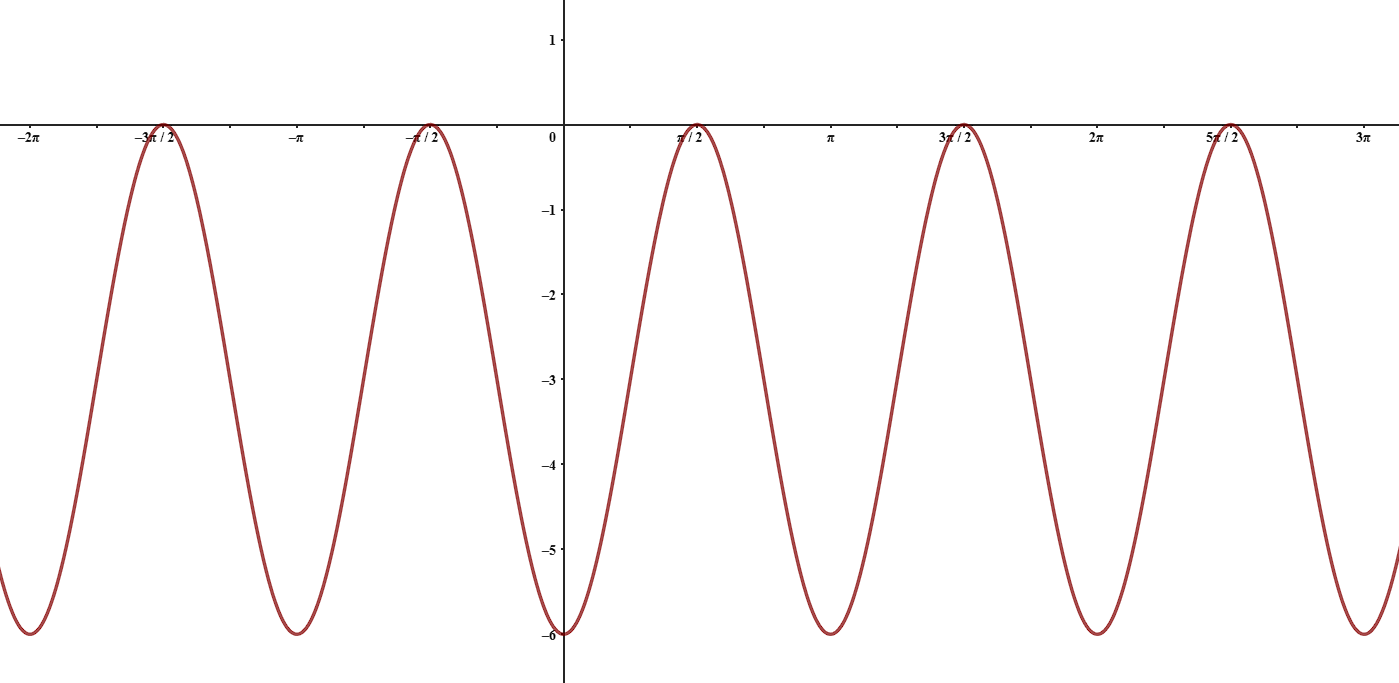
\includegraphics[scale=0.3]{Slike in skice/vaje_vaje_vaje_sinus.png}
    %             \end{figure}
    %         \end{exampleblock}

    %         \note{Avtorica nalog: Darja Turk}

    %     \end{frame}

    %     \begin{frame}
    %         \only<1->{\begin{exampleblock}{Naloga 5}
    %             Brez uporabe računala natančno izračunaj. Zapiši vmesne izračune.
    %             \begin{enumerate}[a]
    %                 \item $\displaystyle \sin\frac{23\pi}{6}$
    %                 \item $\displaystyle \cos\left(-1590^\circ\right)$
    %             \end{enumerate}
    %         \end{exampleblock}}

    %         \only<2->{\begin{exampleblock}{Naloga 6}
    %             Reši enačbi:
    %             \begin{enumerate}[a]
    %                 \item $\displaystyle \sin{2x}+\sqrt{2}\cos x=0$
    %                 \item $\displaystyle 2\cos^2{3x}-\cos{3x}-1=0$
    %             \end{enumerate}
    %         \end{exampleblock}}

    %         \note{Avtorica nalog: Darja Turk}

    %     \end{frame}


    % \subsection{Naklonski kot premice, kot med dvema premicama}
        
    %     \begin{frame}
    %         \frametitle{Naklonski kot premice, kot med dvema premicama}
    %     \end{frame}
% \chapter{Vektorji}
\chapter{Potence in koreni}




    \section{Koreni poljubnih stopenj}

        
            \subsection{Kvadratni koren}

                \textbf{Kvadratni koren} $\sqrt{a}$ realnega števila $a\geq 0$ je tisto nenegativno realno število $x$,
                katerega kvadrat je enak $a$.
                $$\sqrt{a}=x \Leftrightarrow a=x^2; \quad a,x\in\mathbb{R}^+ $$

                Število $a$ imenujemo \textbf{korenjenec}, simbol $\sqrt{~}$ pa \textbf{korenski znak}.
            

            \subsubsection*{Pravila za računanje s kvadratnimi koreni}
                    \begin{multicols}{2}
                        \begin{itemize}
                            \item $\left(\sqrt{a}\right)^2=a; ~a\geq 0$
                            \item $\sqrt{a^2}=\begin{cases}
                                a, & a\geq 0 \\
                                -a, & a<0
                            \end{cases}=\lvert a\rvert$
                            \item $\sqrt{a\cdot b}=\sqrt{a}\cdot\sqrt{b}; ~a,b\geq 0$
                            \item $\sqrt{\dfrac{a}{b}}=\dfrac{\sqrt{a}}{\sqrt{b}}; ~a\geq 0, b>0$
                        \end{itemize}
                    \end{multicols}
                    
            

        

        
            \subsection{Kubični koren}

                \textbf{Kubični koren} $\sqrt[3]{a}$ realnega števila $a$ je tisto realno število $x$,
                katerega kub je enak $a$.
                $$\sqrt[3]{a}=x \Leftrightarrow a=x^3; \quad a,x\in\mathbb{R}$$

                Število $a$ imenujemo \textbf{korenjenec}, simbol $\sqrt{~}$ \textbf{korenski znak}, število $3$ pa \textbf{korenski eksponent}.
            

            \subsubsection*{Pravila za računanje s kubičnimi koreni}
                \begin{multicols}{2}
                    \begin{itemize}
                        \item $\left(\sqrt[3]{a}\right)^3=a$
                        \item $\sqrt[3]{a^3}=a$
                        \item $\sqrt[3]{a\cdot b}=\sqrt[3]{a}\cdot\sqrt[3]{b}$
                        \item $\sqrt[3]{\dfrac{a}{b}}=\dfrac{\sqrt[3]{a}}{\sqrt[3]{b}}; ~b\neq 0$
                    \end{itemize}
                \end{multicols}
                
            

        


        
            \subsection{Koreni poljubnih stopenj}

                Za sodo naravno število $n$ je \textbf{$n$-ti koren} $\sqrt[n]{a}$ realnega števila $a\geq 0$ tisto nenegativno realno število $x$,
                za katerega velja $a=x^n$.
                $$\displaystyle \sqrt[n]{a}=x \Leftrightarrow a=x^n; \quad a,x\in\mathbb{R}^+ $$
                ~
                
                Za liho naravno število $n$ je \textbf{$n$-ti koren} $\sqrt[n]{a}$ realnega števila $a$ tisto realno število $x$,
                za katerega velja $a=x^n$.
                $$\displaystyle \sqrt[n]{a}=x \Leftrightarrow a=x^n; \quad a,x\in\mathbb{R} $$
                ~
                
                Število $a$ imenujemo \textbf{korenjenec}, simbol $\sqrt{~}$ \textbf{korenski znak}, število $n$ pa \textbf{korenski eksponent}.
            

        

         
                        
            \subsubsection*{Pravila za računanje s koreni poljubnih stopenj}
                \begin{multicols}{2}
                    \begin{itemize}
                        \item $\displaystyle \left(\sqrt[n]{a}\right)^n=a$ 
                        \item $\displaystyle \sqrt[n]{a^n}=\begin{cases}
                                \lvert a\rvert, & n=2k, k\in\mathbb{N} \\
                                a, & n=2k-1, k\in\mathbb{N}
                            \end{cases}$ ~
                        \item $\displaystyle \sqrt[n]{a^w}=\left(\sqrt[n]{a}\right)^w$ 
                        \item $\displaystyle \sqrt[n]{a^w}=\sqrt[nz]{a^{wz}}$ 
                        \item $\displaystyle \sqrt[n]{\sqrt[m]{a}}=\sqrt[nm]{a}$ 
                        \item $\displaystyle \sqrt[n]{a\cdot b}=\sqrt[n]{a}\cdot\sqrt[n]{b}$ 
                        \item $\displaystyle \sqrt[n]{\dfrac{a}{b}}=\dfrac{\sqrt[n]{a}}{\sqrt[n]{b}}; ~b\neq 0$ 
                        \item $\displaystyle \sqrt[n]{a^w}\cdot\sqrt[n]{a^z}=\sqrt[n]{a^{w+z}}$ 
                        \item $\displaystyle \dfrac{\sqrt[n]{a^w}}{\sqrt[n]{a^z}}=\sqrt[n]{a^{w-z}}; ~a\neq 0$
                    \end{itemize}

                \end{multicols}
                
                

                Pri tem za sode korenske stopnje $n$ privzamemo $a,b\in[0,\infty)$; za lihe stopnje $n$ pa $a,b\in\mathbb{R}$.
            

        
                ~\\~\\~

    %%% naloge

        
            \begin{naloga}
                Poenostavite izraz in ga delno korenite.
                \begin{multicols}{2}
                    \begin{itemize}
                        \item $\displaystyle \sqrt[3]{xy^2\sqrt{x^5y}}$ 
                        \item $\displaystyle \sqrt{a\sqrt{a^2\sqrt{a^3}}}$ 
                        \item $\displaystyle \sqrt[4]{a^3b^2\sqrt{ab^5}}$ 
                        \item $\displaystyle \sqrt[4]{ab^2\sqrt[3]{ab}}$ 
                        \item $\displaystyle \sqrt[3]{a\sqrt[4]{a\sqrt[5]{a}}}$ 
                        \item $\displaystyle \sqrt[5]{x^4y\sqrt[4]{x^5y^3}}$ 
                        \item $\displaystyle \sqrt[6]{a^2b^3\sqrt{a^8\sqrt[3]{b}}}$    
                        \item $\displaystyle \sqrt[3]{x\sqrt{y^3\sqrt[4]{x^3\sqrt[5]{y^6y^{-1}}}}}$                  
                    \end{itemize}
                \end{multicols}
            \end{naloga}
        


        
            \begin{naloga}
                Izračunajte.
                \begin{multicols}{2}
                    \begin{itemize}
                        \item $\displaystyle \sqrt[5]{\dfrac{1}{32}}$ 
                        \item $\displaystyle \sqrt[4]{\dfrac{16}{81}}$ 
                        \item $\displaystyle \sqrt[3]{-8}$ 
                        \item $\displaystyle \sqrt[4]{-625}$ 
                        \item $\displaystyle \sqrt[3]{0.125}$ 
                        \item $\displaystyle \sqrt[4]{0.0016}$ 
                    \end{itemize}
                \end{multicols}
            \end{naloga}
        
        
            \begin{naloga}
                Poenostavite.
                \begin{itemize}
                    \item $\displaystyle \sqrt[18]{x^{15}}$ 
                    \item $\displaystyle \sqrt[9]{a^6}$ 
                    \item $\displaystyle \sqrt[30]{y^{18}}$ 
                    \item $\displaystyle \sqrt[20]{b^{30}}$ 
                \end{itemize}
            \end{naloga}
        
        
            \begin{naloga}
                Racionalizirajte ulomke.
                \begin{multicols}{2}
                    \begin{itemize}
                        \item $\displaystyle \dfrac{1}{3-\sqrt{x}}$ 
                        \item $\displaystyle \dfrac{1}{2-4\sqrt[3]{a}}$ 
                        \item $\displaystyle \dfrac{2}{a-\sqrt[3]{b}}$ 
                        \item $\displaystyle \dfrac{x-1}{\sqrt[3]{x}-1}$ 
                        \item $\displaystyle \dfrac{8x}{2\sqrt[3]{x}+1}$ 
                        \item $\displaystyle \dfrac{1}{2-\sqrt[4]{3}}$ 
                        \item $\displaystyle \dfrac{1}{\sqrt[4]{2}-1}$ 
                        \item $\displaystyle \dfrac{\sqrt[4]{y}}{2-\sqrt[4]{y}}$ 
                        \item $\displaystyle \dfrac{3}{1+\sqrt[5]{2}}$ 
                    \end{itemize}
                \end{multicols}
            \end{naloga}
        
        
            \begin{naloga}
                Poenostavite in delno korenite izraz.
                \begin{multicols}{2}
                    \begin{itemize}
                        \item $\displaystyle \dfrac{\sqrt[4]{2}}{\sqrt{2\sqrt{8}}}$ 
                        \item $\displaystyle \dfrac{\sqrt[3]{9}}{\sqrt[5]{3}\sqrt{27}}$ 
                        \item $\displaystyle \dfrac{\sqrt{\sqrt{\sqrt{1}}}}{\sqrt[17]{1}}$ 
                        \item $\displaystyle \dfrac{\sqrt{\sqrt{a}}}{\sqrt[3]{a^2}}$ 
                        \item $\displaystyle \dfrac{\sqrt{a\sqrt[3]{a^{-1}}\cdot\sqrt[3]{a^2\sqrt[5]{a}}}}{\sqrt[5]{a\sqrt{a^{-5}}}}$ 
                        \item $\displaystyle \dfrac{\sqrt{x^3\sqrt[4]{x^3\sqrt{x}}}}{\sqrt[4]{x^{-3}\sqrt[4]{x}}}$ 
                        \item $\displaystyle \dfrac{\sqrt[7]{b^{13}\sqrt{b^{-2}}}}{\sqrt{\sqrt{b^{-1}}}}$ 
                        \item $\displaystyle \dfrac{\sqrt[3]{x^2\sqrt[4]{x^{-1}}}\cdot\sqrt[4]{x^3\sqrt{x}}}{\sqrt[4]{x\sqrt{x\sqrt[3]{x^{-1}}}}}$ 
                        \item $\displaystyle \dfrac{\sqrt{8ab^{-1}}}{\sqrt{0.5}\sqrt[3]{8ab^2}}$ 
                    \end{itemize}
                \end{multicols}
            \end{naloga}
        
        
            \begin{naloga}
                Izračunajte natančno vrednost korena.
                \begin{itemize}
                    \item $\displaystyle \sqrt{31-12\sqrt{3}}$ 
                    \item $\displaystyle \sqrt{18+8\sqrt{2}}$ 
                    \item $\displaystyle \sqrt{9-4\sqrt{5}}$ 
                    \item $\displaystyle \sqrt{17+2\sqrt{2}}$ 
                \end{itemize}
                
            \end{naloga}
        
        
            \begin{naloga}
                Poenostavite izraz in ga delno korenite.
                \begin{multicols}{2}
                    \begin{itemize}
                        \item $\displaystyle \dfrac{\sqrt[5]{xy^3\sqrt[4]{x^2y^3}}}{\sqrt[10]{\sqrt{x}}}$ 
                        \item $\displaystyle \dfrac{\sqrt[4]{ab^3\sqrt[3]{a^2b^3}}}{\sqrt{\sqrt[6]{a}}}$ 
                        \item $\displaystyle \left(\dfrac{1-z}{1-\sqrt[3]{z}}-\sqrt[3]{z}\right)\left(1-\sqrt[6]{z^4}\right)$ 
                        \item $\displaystyle \sqrt[3]{\sqrt{\sqrt{4096}}}+\sqrt{\sqrt{\sqrt{16}}}-\sqrt[5]{32}$ 
                        \item $\displaystyle \dfrac{\sqrt[6]{ab^3\sqrt{a^3b}}}{\sqrt[4]{b^{-3}\sqrt[3]{a}}}$ 
                    \end{itemize}
                \end{multicols}
            \end{naloga}
        



            \newpage
    \section{Potence z racionalnimi eksponenti}

        
            \subsection{Potence z racionalnimi eksponenti}

            Potenca z racionalnim eksponentom je definirana kot: 
                $$\displaystyle x^\frac{m}{n}=\sqrt[n]{x^m},$$
                kjer je $m\in\mathbb{Z}$, $n\in\mathbb{N}$ in $a\in[0,\infty)$.
            

            \subsubsection*{Pravila za računanje s potencami s celimi eksponenti}
                
                        \begin{itemize}
                            \item $\displaystyle x^p\cdot x^q=x^{p+q}$
                            \item $\displaystyle x^p\cdot y^p=(xy)^p$
                            \item $\displaystyle \left(x^p\right)^q=x^{pq}$
                        \end{itemize}
                        \begin{itemize}
                            \item $\displaystyle x^p:x^q=\dfrac{x^p}{x^q}=x^{p-q}; \quad x\neq 0$
                            \item $\displaystyle x^p:y^p=\dfrac{x^p}{y^p}=\left(\dfrac{x}{y}\right)^p; \quad y\neq 0$
                        \end{itemize}
                
                ~

                V pravilih upoštevamo primerni realni osnovi $x,y\in\mathbb{R}$ in racionalne eksponente $p,q\in\mathbb{Q}$.



    %%% naloge

            \begin{naloga}
                Izračunajte.
                \begin{itemize}
                    \item $\displaystyle 8^\frac{1}{3}-16^\frac{2}{4}$ 
                    \item $\displaystyle 27^\frac{2}{3}-125^\frac{1}{3}$ 
                    \item $\displaystyle \left(-8\right)^{-\frac{1}{3}}$ 
                    \item $\displaystyle 1000^\frac{2}{3}-343^\frac{2}{3}$ 
                \end{itemize}
            \end{naloga}

            
            \begin{naloga}
                Izračunajte.
                \begin{multicols}{2}
                    \begin{itemize}
                        \item $\displaystyle \sqrt{625^\frac{3}{4}-\left(\dfrac{1}{2}\right)^{-2}}+4^\frac{1}{3}\cdot 16^\frac{1}{3} $ 
                        \item $\displaystyle 4\cdot 0.16^{-\frac{1}{2}}-\sqrt[3]{5\cdot 8^\frac{1}{3}+2\cdot 81^\frac{3}{4}} $ 
                        \item $\displaystyle \left(2\cdot 9^\frac{3}{2}+5\cdot 16^\frac{1}{4}\right)^\frac{1}{3} $ 
                        \item $\displaystyle \left(\left(\dfrac{4}{9}\right)^{-\frac{1}{2}}\cdot 32^\frac{1}{5}+169^\frac{1}{2}\right)^\frac{1}{2} $ 
                        \item $\displaystyle 0.25^{-\frac{1}{2}}\cdot 0.001^{-\frac{1}{3}} -\sqrt[3]{10^2+0.2^{-2}} $ 
                        \item $\displaystyle \left(3\dfrac{3}{8}\right)^\frac{2}{3}\cdot\left(\dfrac{1}{4}\right)^{-\frac{1}{2}}\cdot\left(3-\sqrt{5}\right)\sqrt{7+3\sqrt{5}} $ 
                    \end{itemize}
                \end{multicols}
            \end{naloga}
        
        
            \begin{naloga}
                Izračunajte.
                \begin{multicols}{2}
                    \begin{itemize}
                        \item $\displaystyle 2.25^{-0.5}\cdot\sqrt{4^{1.5}+1} $ 
                        \item $\displaystyle 6.25^{-0.5}\cdot 2.25^{1.5}+\sqrt{16^{0.75}+1} $ 
                        \item $\displaystyle \left(3\dfrac{1}{16}\right)^{-0.5}\sqrt{0.125^{-\frac{2}{3}}+3}^4+0.002^{-\frac{2}{3}} $ 
                        \item $\displaystyle \sqrt{10}\left(5^{-0.5}-2\right)^{-1}-\sqrt{90} $ 
                        \item $\displaystyle \sqrt{27^\frac{2}{3}+0.25^{-2}}+\left(2-\sqrt{5}\right)\sqrt{9+4\sqrt{5}}-\dfrac{1+\sqrt{12}}{2+\sqrt{3}} $ 
                    \end{itemize}
                \end{multicols}
            \end{naloga}

        
            \begin{naloga}
                Izraz zapišite s potencami in ga poenostavite.
                \begin{multicols}{2}
                    \begin{itemize}
                        \item $\displaystyle \left(\dfrac{1-z}{1-\sqrt[3]{z}}-\sqrt[3]{z}\right)\left(1-\sqrt[6]{z^4}\right)$ 
                        \item $\displaystyle \dfrac{\sqrt[6]{ab^3\sqrt{a^3b}}}{\sqrt[4]{b^{-3}\sqrt[3]{a}}}$ 
                        \item $\displaystyle \left(y^\frac{2}{3}x^{-0.25}\right)^6 :\left(\sqrt{x^{-4}y^2}\cdot\sqrt{y\sqrt[3]{xy^{-3}}}\right)^3 $ 
                        \item $\displaystyle \dfrac{\sqrt[3]{x^{-4}\sqrt{x^2y^{-3}}}}{\sqrt[4]{x^{-3}y^2}}\cdot\left(x^{0.3}y^{0.2}\right)^5 $ 
                        \item $\displaystyle \dfrac{\sqrt[5]{x^{-2}\sqrt[3]{x^{-3}y^4}}}{y^{-\frac{1}{3}}x^\frac{1}{2}}\left(\sqrt[6]{\sqrt{y^{-3}}}\right)^4 $ 
                        \item $\displaystyle \dfrac{\sqrt[4]{x^{-2}y}}{\sqrt[6]{x^3\sqrt{y^{-7}}}}\sqrt[4]{x^2y^{-5}}^2 $ 
                    \end{itemize}
                \end{multicols}
            \end{naloga}
        





            \newpage

    \section{Iracionalne enačbe}

        
            \subsection{Iracionalne enačbe}

                \textbf{Iracionalna enačba} je enačba, v kateri neznanka nastopa po korenom poljubne stopnje.
            

            \subsubsection*{Reševanje iracionalne enačbe}
                Iracionalno enačbo rešujemo tako, da jo s pomočjo potenciranja prevedemo v enačbo, ki nima neznanke pod korenom.

                Tako dobimo enačbo, ki ni nujno ekvivalentna prvotni enačba, saj lahko s potenciranjem pridobimo kakšno rešitev, ki ne ustreza prvotni enačbo.

                Na koncu reševanja moramo vedno narediti \textbf{preizkus}, s katerim izločimo morebitne neustrezne rešitve.
            
        


    %%% naloge

        
            \begin{naloga}
                Rešite enačbo.
                \begin{itemize}
                    \item $\displaystyle \sqrt{x-1}-5=0$ 
                    \item $\displaystyle \sqrt{x+5}=2$ 
                    \item $\displaystyle \sqrt{3-x}-5=0$ 
                    \item $\displaystyle 1+\sqrt{x-5}=0$ 
                \end{itemize}
            \end{naloga}

        
            \begin{naloga}
                Rešite enačbo.
                \begin{multicols}{2}
                    \begin{itemize}
                        \item $\displaystyle \sqrt{2x-1}+2x=x$ 
                        \item $\displaystyle 2+\sqrt[3]{x-1}=0$ 
                        \item $\displaystyle \sqrt{x^2+2}-\sqrt{3x}=0$ 
                        \item $\displaystyle x-\sqrt{5x-11}=1$ 
                        \item $\displaystyle 2x+3=\sqrt{3x^2+5x-1}$ 
                        \item $\displaystyle \sqrt{-8x-4}=-2x$ 
                        \item $\displaystyle \sqrt{x^2-1}-2=0$ 
                        \item $\displaystyle \sqrt{x+3}=-9$ 
                    \end{itemize}
                \end{multicols}
            \end{naloga}

        
            \begin{naloga}
                Rešite enačbo.
                \begin{multicols}{2}
                    \begin{itemize}
                        \item $\displaystyle \sqrt{x}+\sqrt{x+1}=3$ 
                        \item $\displaystyle \sqrt{x-2}-2=\sqrt{x+2}$ 
                        \item $\displaystyle \sqrt{x+1}=\sqrt{2}-\sqrt{x-1}$ 
                        \item $\displaystyle \sqrt{x-6}+\sqrt{x+2}=2$ 
                        \item $\displaystyle \sqrt{x+5}-3=-\sqrt{x}$ 
                        \item $\displaystyle \sqrt{3x+1}-1=\sqrt{x+4}$ 
                        \item $\displaystyle \sqrt[3]{x+2-\sqrt{10+x}}=-2$ 
                        \item $\displaystyle \sqrt{5+x}-1=\sqrt{3x+4}$ 
                    \end{itemize}
                \end{multicols}
            \end{naloga}

        
            \begin{naloga}
                Rešite enačbo.
                \begin{multicols}{2}
                    \begin{itemize}
                        \item $\displaystyle \sqrt[3]{x^3+7x^2+x+26}-3=x-1$ 
                        \item $\displaystyle \sqrt{x-2}-\sqrt{2x-3}=2$ 
                        \item $\displaystyle \sqrt{x^2+3x}+x=2$ 
                        \item $\displaystyle \sqrt{x+7-\sqrt{2x-1}}=3$ 
                        \item $\displaystyle \sqrt[3]{5-x+\sqrt{2x+14}}-2=0$ 
                        \item $\displaystyle \sqrt{x-6}-\sqrt{x+2}-2=0$ 
                        \item $\displaystyle \sqrt{x+3+\sqrt{x+2}}=\sqrt{3}$ 
                        \item $\displaystyle \sqrt[5]{x^2+3x+34}=2$ 
                    \end{itemize}
                \end{multicols}
            \end{naloga}
        

% \chapter{Funkcija}
% \chapter{Potenčna funkcija}
% \chapter{Korenska funkcija}
% \section{Kvadratna funkcija}

\begin{frame}
    \sectionpage
\end{frame}

\begin{frame}
    \tableofcontents[currentsection, hideothersubsections]
\end{frame}

    \subsection{Kvadratna enačba}

        \begin{frame}
            \frametitle{Kvadratna enačba}
        \end{frame}

    \subsection{Kvadratna funkcija in parabola}

        \begin{frame}
            \frametitle{Kvadratna funkcija in parabola}
        \end{frame}

    \subsection{Presečišča parabol}

        \begin{frame}
            \frametitle{Presečišča parabol}
        \end{frame}

    \subsection{Kvadratna neenačba}

        \begin{frame}
            \frametitle{Kvadratna neenačba}
        \end{frame}

    \subsection{Modeliranje s kvadratno funkcijo in ekstremalni problemi}

        \begin{frame}
            \frametitle{Modeliranje s kvadratno funkcijo in ekstremalni problemi}
        \end{frame}

    \subsection{Množica kompleksnih števil}

        \begin{frame}
            \frametitle{Množica kompleksnih števil}
        \end{frame}

    \subsection{Računanje s kompleksnimi števili}

        \begin{frame}
            \frametitle{Računanje s kompleksnimi števili}
        \end{frame}

% \chapter{Kompleksna števila}
% \section{Eksponentna funkcija}

\begin{frame}
    \sectionpage
\end{frame}

\begin{frame}
    \tableofcontents[currentsection, hideothersubsections]
\end{frame}

    \subsection{Eksponentna enačba}

        \begin{frame}
            \frametitle{Eksponentna enačba}

            \textbf{Štirje tipi eksponentne enačbe:}
            \begin{enumerate}
                \item z enako osnovo: $$\mathbf{a^{f(x)}=a^{g(x)}} \Rightarrow \mathbf{f(x)=g(x)}$$
                \item z različno osnovo in enakimi eksponenti:  $$\mathbf{a^{f(x)}=b^{f(x)}}, a\neq b \Rightarrow \mathbf{f(x)=0}$$
                \item z različno osnovo in različnima eksponentoma: $$\mathbf{a^{f(x)}=c}; c\in\mathbb{R} \Rightarrow \textrm{reševanje z logaritmom}$$
                \item $$\mathbf{a^{f(x)}=g(x)} \Rightarrow \textrm{grafično reševanje}$$
            \end{enumerate}

        \end{frame}

    \subsection{Logaritem}

        \begin{frame}
            \frametitle{Logaritem}

            \textbf{Logaritem} z osnovo $a$ števila $x$ je tisti eksponent, pri katerem je potenca z osnovo $a$ enaka $x$: $$y=\log_ax \Leftrightarrow a^y=x.$$

            V zapisu $\log_ax$ imenujemo število $x$ \textbf{logaritmand}, število $a$ pa \textbf{osnova logaritma}. Le-ta je pozitivna in različna od $1$.

            Logaritem z osnovo $e$ imenujemo \textbf{naravni logaritem} in ga označimo z $\ln$: $\log_ex=\ln x$.
            Logaritem z osnovo $10$ imenujemo \textbf{desetiški logaritem} in ga označimo z $\log$: $\log_{10}x=\log x$.

        \end{frame}

        \begin{frame}
            \large\textbf{Lastnosti logaritmov}
            ~\\
            \normalsize

            \begin{alertblock}{}
                $$\log_a1=0$$
            \end{alertblock}

            \begin{alertblock}{}
                $$\log_aa=1$$
            \end{alertblock}

            \begin{alertblock}{}
                $$\log_aa^x=x, \textrm{\ kjer je\ } x\in\mathbb{R}$$
            \end{alertblock}

            \begin{alertblock}{}
                $$a^{\log_ax}=x, \textrm{\ kjer je\ } x>0$$
            \end{alertblock}
        \end{frame}

    \subsection{Pravila za računanje z logaritmi}

        \begin{frame}
            \frametitle{Pravila za računanje z logaritmi}
        
            \begin{alertblock}{}
                $$\log_axy = \log_ax + \log_ay$$
                $$\log_a\frac{x}{y} = \log_ax - \log_ay$$
            \end{alertblock}

            \begin{alertblock}{}
                $$\log_ax^n = n\log_ax$$
                $$\log_a\sqrt[n]{x} = \frac{1}{n}\log_ax$$
            \end{alertblock}

            \begin{alertblock}{Prehod k novi osnovi}
                $$\log_ax = \frac{\log_bx}{\log_ba}$$
            \end{alertblock}


        \end{frame}

    \subsection{Logaritemska enačba}

        \begin{frame}[t]
            \frametitle{Logaritemska enačba}

            Enačba je logaritemska, če v njej nastopa neznanka v osnovi ali v logaritmandu vsaj enega logaritma.\\
            ~\\
            Reševanje logaritemske enačbe:
            \begin{itemize}
                \item z uporabo definicije;
                \item s pravili za logaritmiranje;
                \item s prehodom k isti osnovi;
                \item z uvedbo nove neznanke;
                \item grafično reševanje.
            \end{itemize}


        \end{frame}

    \subsection{Eksponentna in logaritemska funkcija}

        \begin{frame}[t]
            \frametitle{Eksponentna in logaritemska funkcija}
            \large\textbf{Eksponentna funkcija}
            ~\\
            \normalsize

            \begin{columns}
                \column{0.6\textwidth}
                    \begin{alertblock}{}
                        \textbf{Eksponentna funkcija} je realna funkcija oblike:
                        $$\mathbf{f(x)=a^x}, \textrm{\ kjer je\ } a>0 \wedge a\neq 1. $$
                        Število $a$ imenujemo \textbf{osnova} eksponentne funkcije.
                    \end{alertblock}

                    ~\\
                    Kot poseben primer eksponentne funkcije velja \textbf{naravna eksponentna funkcija} $f(x)=e^x$. To je eksponentna funkcija, ki ima za osnovo Eulerjevo število $e=2,71828…$.
        
                \column{0.38\textwidth}
                    \begin{figure}
                        \begin{tikzpicture}
                            % \clip (0,0) rectangle (14.000000,10.000000);
                            {\footnotesize
                            
                            % Drawing 2D Cartesian system
                            \draw (3.000000,1.500000) node [anchor=north east] { $0$ };%
                            \draw [line width=0.016cm] (3.000000,1.425000) -- (3.000000,1.575000);%
                            \draw (3.500000,1.500000) node [anchor=north] { $1$ };%
                            \draw [line width=0.016cm] (3.500000,1.425000) -- (3.500000,1.575000);%
                            \draw (4.000000,1.500000) node [anchor=north] { $2$ };%
                            \draw [line width=0.016cm] (4.000000,1.425000) -- (4.000000,1.575000);%
                            \draw (4.500000,1.500000) node [anchor=north] { $3$ };%
                            \draw [line width=0.016cm] (4.500000,1.425000) -- (4.500000,1.575000);%
                            \draw (2.500000,1.500000) node [anchor=north] { $-1$ };%
                            \draw [line width=0.016cm] (2.500000,1.425000) -- (2.500000,1.575000);%
                            \draw (2.000000,1.500000) node [anchor=north] { $-2$ };%
                            \draw [line width=0.016cm] (2.000000,1.425000) -- (2.000000,1.575000);%
                            \draw (1.500000,1.500000) node [anchor=north] { $-3$ };%
                            \draw [line width=0.016cm] (1.500000,1.425000) -- (1.500000,1.575000);%
                            \draw (1.000000,1.500000) node [anchor=north] { $-4$ };%
                            \draw [line width=0.016cm] (1.000000,1.425000) -- (1.000000,1.575000);%
                            \draw (3.000000,2.000000) node [anchor=east] { $1$ };%
                            \draw [line width=0.016cm] (2.925000,2.000000) -- (3.075000,2.000000);%
                            \draw (3.000000,2.500000) node [anchor=east] { $2$ };%
                            \draw [line width=0.016cm] (2.925000,2.500000) -- (3.075000,2.500000);%
                            \draw (3.000000,3.000000) node [anchor=east] { $3$ };%
                            \draw [line width=0.016cm] (2.925000,3.000000) -- (3.075000,3.000000);%
                            \draw (3.000000,3.500000) node [anchor=east] { $4$ };%
                            \draw [line width=0.016cm] (2.925000,3.500000) -- (3.075000,3.500000);%
                            \draw (3.000000,4.000000) node [anchor=east] { $5$ };%
                            \draw [line width=0.016cm] (2.925000,4.000000) -- (3.075000,4.000000);%
                            \draw (3.000000,4.500000) node [anchor=east] { $6$ };%
                            \draw [line width=0.016cm] (2.925000,4.500000) -- (3.075000,4.500000);%
                            \draw (3.000000,1.000000) node [anchor=east] { $-1$ };%
                            \draw [line width=0.016cm] (2.925000,1.000000) -- (3.075000,1.000000);%
                            \draw (4.900000,1.500000) node [anchor=south] { $x$ };%
                            \draw (3.000000,4.900000) node [anchor=west] { $y$ };%
                            \draw [line width=0.016cm] (0.800000,1.500000) -- (4.900000,1.500000);%
                            \draw [line width=0.016cm] (4.602567,1.539158) -- (4.900000,1.500000);%
                            \draw [line width=0.016cm] (4.602567,1.539158) -- (4.800000,1.500000);%
                            \draw [line width=0.016cm] (4.602567,1.460842) -- (4.900000,1.500000);%
                            \draw [line width=0.016cm] (4.602567,1.460842) -- (4.800000,1.500000);%
                            \draw [line width=0.016cm] (3.000000,0.600000) -- (3.000000,4.900000);%
                            \draw [line width=0.016cm] (2.960842,4.602567) -- (3.000000,4.900000);%
                            \draw [line width=0.016cm] (2.960842,4.602567) -- (3.000000,4.800000);%
                            \draw [line width=0.016cm] (3.039158,4.602567) -- (3.000000,4.900000);%
                            \draw [line width=0.016cm] (3.039158,4.602567) -- (3.000000,4.800000);%
                            
                            % Changing color 255 0 0
                            \definecolor{r255g0b0}{rgb}{1.000000,0.000000,0.000000}%
                            \color{r255g0b0}% 
                            
                            % Drawing 2D parametric curve (x,exp(x))
                            \draw [line width=0.032cm] (0.850000,1.506784) -- (0.800000,1.506139);%
                            \draw [line width=0.032cm] (0.900000,1.507498) -- (0.850000,1.506784);%
                            \draw [line width=0.032cm] (0.950000,1.508286) -- (0.900000,1.507498);%
                            \draw [line width=0.032cm] (1.000000,1.509158) -- (0.950000,1.508286);%
                            \draw [line width=0.032cm] (1.050000,1.510121) -- (1.000000,1.509158);%
                            \draw [line width=0.032cm] (1.100000,1.511185) -- (1.050000,1.510121);%
                            \draw [line width=0.032cm] (1.150000,1.512362) -- (1.100000,1.511185);%
                            \draw [line width=0.032cm] (1.200000,1.513662) -- (1.150000,1.512362);%
                            \draw [line width=0.032cm] (1.250000,1.515099) -- (1.200000,1.513662);%
                            \draw [line width=0.032cm] (1.300000,1.516687) -- (1.250000,1.515099);%
                            \draw [line width=0.032cm] (1.350000,1.518442) -- (1.300000,1.516687);%
                            \draw [line width=0.032cm] (1.400000,1.520381) -- (1.350000,1.518442);%
                            \draw [line width=0.032cm] (1.450000,1.522525) -- (1.400000,1.520381);%
                            \draw [line width=0.032cm] (1.500000,1.524894) -- (1.450000,1.522525);%
                            \draw [line width=0.032cm] (1.550000,1.527512) -- (1.500000,1.524894);%
                            \draw [line width=0.032cm] (1.600000,1.530405) -- (1.550000,1.527512);%
                            \draw [line width=0.032cm] (1.650000,1.533603) -- (1.600000,1.530405);%
                            \draw [line width=0.032cm] (1.700000,1.537137) -- (1.650000,1.533603);%
                            \draw [line width=0.032cm] (1.750000,1.541042) -- (1.700000,1.537137);%
                            \draw [line width=0.032cm] (1.800000,1.545359) -- (1.750000,1.541042);%
                            \draw [line width=0.032cm] (1.850000,1.550129) -- (1.800000,1.545359);%
                            \draw [line width=0.032cm] (1.900000,1.555402) -- (1.850000,1.550129);%
                            \draw [line width=0.032cm] (1.950000,1.561228) -- (1.900000,1.555402);%
                            \draw [line width=0.032cm] (2.000000,1.567668) -- (1.950000,1.561228);%
                            \draw [line width=0.032cm] (2.050000,1.574784) -- (2.000000,1.567668);%
                            \draw [line width=0.032cm] (2.100000,1.582649) -- (2.050000,1.574784);%
                            \draw [line width=0.032cm] (2.150000,1.591342) -- (2.100000,1.582649);%
                            \draw [line width=0.032cm] (2.200000,1.600948) -- (2.150000,1.591342);%
                            \draw [line width=0.032cm] (2.250000,1.611565) -- (2.200000,1.600948);%
                            \draw [line width=0.032cm] (2.300000,1.623298) -- (2.250000,1.611565);%
                            \draw [line width=0.032cm] (2.350000,1.636266) -- (2.300000,1.623298);%
                            \draw [line width=0.032cm] (2.400000,1.650597) -- (2.350000,1.636266);%
                            \draw [line width=0.032cm] (2.450000,1.666436) -- (2.400000,1.650597);%
                            \draw [line width=0.032cm] (2.500000,1.683940) -- (2.450000,1.666436);%
                            \draw [line width=0.032cm] (2.550000,1.703285) -- (2.500000,1.683940);%
                            \draw [line width=0.032cm] (2.600000,1.724664) -- (2.550000,1.703285);%
                            \draw [line width=0.032cm] (2.650000,1.748293) -- (2.600000,1.724664);%
                            \draw [line width=0.032cm] (2.700000,1.774406) -- (2.650000,1.748293);%
                            \draw [line width=0.032cm] (2.750000,1.803265) -- (2.700000,1.774406);%
                            \draw [line width=0.032cm] (2.800000,1.835160) -- (2.750000,1.803265);%
                            \draw [line width=0.032cm] (2.850000,1.870409) -- (2.800000,1.835160);%
                            \draw [line width=0.032cm] (2.900000,1.909365) -- (2.850000,1.870409);%
                            \draw [line width=0.032cm] (2.950000,1.952419) -- (2.900000,1.909365);%
                            \draw [line width=0.032cm] (3.000000,2.000000) -- (2.950000,1.952419);%
                            \draw [line width=0.032cm] (3.050000,2.052585) -- (3.000000,2.000000);%
                            \draw [line width=0.032cm] (3.100000,2.110701) -- (3.050000,2.052585);%
                            \draw [line width=0.032cm] (3.150000,2.174929) -- (3.100000,2.110701);%
                            \draw [line width=0.032cm] (3.200000,2.245912) -- (3.150000,2.174929);%
                            \draw [line width=0.032cm] (3.250000,2.324361) -- (3.200000,2.245912);%
                            \draw [line width=0.032cm] (3.300000,2.411059) -- (3.250000,2.324361);%
                            \draw [line width=0.032cm] (3.350000,2.506876) -- (3.300000,2.411059);%
                            \draw [line width=0.032cm] (3.400000,2.612770) -- (3.350000,2.506876);%
                            \draw [line width=0.032cm] (3.450000,2.729802) -- (3.400000,2.612770);%
                            \draw [line width=0.032cm] (3.500000,2.859141) -- (3.450000,2.729802);%
                            \draw [line width=0.032cm] (3.550000,3.002083) -- (3.500000,2.859141);%
                            \draw [line width=0.032cm] (3.600000,3.160058) -- (3.550000,3.002083);%
                            \draw [line width=0.032cm] (3.650000,3.334648) -- (3.600000,3.160058);%
                            \draw [line width=0.032cm] (3.700000,3.527600) -- (3.650000,3.334648);%
                            \draw [line width=0.032cm] (3.750000,3.740845) -- (3.700000,3.527600);%
                            \draw [line width=0.032cm] (3.800000,3.976516) -- (3.750000,3.740845);%
                            \draw [line width=0.032cm] (3.850000,4.236974) -- (3.800000,3.976516);%
                            \draw [line width=0.032cm] (3.900000,4.524824) -- (3.850000,4.236974);%
                            \draw [line width=0.032cm] (3.950000,4.842947) -- (3.900000,4.524824);%
                            \draw [line width=0.032cm] (3.950000,4.842947) -- (3.958114,4.900000);%
                            \color{black}
                            }
                        \end{tikzpicture}                            
                    \end{figure}
            \end{columns}

        \end{frame}

        \begin{frame}[t]

            \begin{columns}
                \column{0.6\textwidth}
                \textbf{Lastnosti eksponentne funkcije:}
                \begin{itemize}
                    \item definicijsko območje predstavljajo vsa realna števila: $\mathcal{D}_f=\mathbb{R}$;
                    \item zaloga vrednosti je množica pozitivnih realnih števil: $\mathcal{Z}_f=(0,\infty)$;
                    \item za $a>1$ je naraščajoča, za $0<a<1$ je padajoča;
                    \item je injektivna;
                    \item vodoravna asimptota grafa funkcije je abscisna os: $y=0$;
                    \item graf funkcije poteka skozi točko $N(0,1)$.
                \end{itemize}

                \column{0.38\textwidth}
                \begin{figure}
                    \begin{tikzpicture}
                        % \clip (0,0) rectangle (14.000000,10.000000);
                        {\footnotesize
                        
                        % Drawing 2D Cartesian system
                        \draw (3.000000,1.500000) node [anchor=north east] { $0$ };%
                        \draw [line width=0.016cm] (3.000000,1.425000) -- (3.000000,1.575000);%
                        \draw (3.500000,1.500000) node [anchor=north] { $1$ };%
                        \draw [line width=0.016cm] (3.500000,1.425000) -- (3.500000,1.575000);%
                        \draw (4.000000,1.500000) node [anchor=north] { $2$ };%
                        \draw [line width=0.016cm] (4.000000,1.425000) -- (4.000000,1.575000);%
                        \draw (4.500000,1.500000) node [anchor=north] { $3$ };%
                        \draw [line width=0.016cm] (4.500000,1.425000) -- (4.500000,1.575000);%
                        \draw (2.500000,1.500000) node [anchor=north] { $-1$ };%
                        \draw [line width=0.016cm] (2.500000,1.425000) -- (2.500000,1.575000);%
                        \draw (2.000000,1.500000) node [anchor=north] { $-2$ };%
                        \draw [line width=0.016cm] (2.000000,1.425000) -- (2.000000,1.575000);%
                        \draw (1.500000,1.500000) node [anchor=north] { $-3$ };%
                        \draw [line width=0.016cm] (1.500000,1.425000) -- (1.500000,1.575000);%
                        \draw (1.000000,1.500000) node [anchor=north] { $-4$ };%
                        \draw [line width=0.016cm] (1.000000,1.425000) -- (1.000000,1.575000);%
                        \draw (3.000000,2.000000) node [anchor=east] { $1$ };%
                        \draw [line width=0.016cm] (2.925000,2.000000) -- (2.960000,2.000000);%
                        \draw [line width=0.016cm] (3.040000,2.000000) -- (3.075000,2.000000);%
                        \draw (3.000000,2.500000) node [anchor=east] { $2$ };%
                        \draw [line width=0.016cm] (2.925000,2.500000) -- (3.075000,2.500000);%
                        \draw (3.000000,3.000000) node [anchor=east] { $3$ };%
                        \draw [line width=0.016cm] (2.925000,3.000000) -- (3.075000,3.000000);%
                        \draw (3.000000,3.500000) node [anchor=east] { $4$ };%
                        \draw [line width=0.016cm] (2.925000,3.500000) -- (3.075000,3.500000);%
                        \draw (3.000000,4.000000) node [anchor=east] { $5$ };%
                        \draw [line width=0.016cm] (2.925000,4.000000) -- (3.075000,4.000000);%
                        \draw (3.000000,4.500000) node [anchor=east] { $6$ };%
                        \draw [line width=0.016cm] (2.925000,4.500000) -- (3.075000,4.500000);%
                        \draw (3.000000,1.000000) node [anchor=east] { $-1$ };%
                        \draw [line width=0.016cm] (2.925000,1.000000) -- (3.075000,1.000000);%
                        \draw (4.900000,1.500000) node [anchor=north] { $x$ };%
                        \draw (3.000000,4.900000) node [anchor=east] { $y$ };%
                        \draw [line width=0.016cm] (0.800000,1.500000) -- (4.900000,1.500000);%
                        \draw [line width=0.016cm] (4.602567,1.539158) -- (4.900000,1.500000);%
                        \draw [line width=0.016cm] (4.602567,1.539158) -- (4.800000,1.500000);%
                        \draw [line width=0.016cm] (4.602567,1.460842) -- (4.900000,1.500000);%
                        \draw [line width=0.016cm] (4.602567,1.460842) -- (4.800000,1.500000);%
                        \draw [line width=0.016cm] (3.000000,0.600000) -- (3.000000,1.960000);%
                        \draw [line width=0.016cm] (3.000000,2.040000) -- (3.000000,4.900000);%
                        \draw [line width=0.016cm] (2.960842,4.602567) -- (3.000000,4.900000);%
                        \draw [line width=0.016cm] (2.960842,4.602567) -- (3.000000,4.800000);%
                        \draw [line width=0.016cm] (3.039158,4.602567) -- (3.000000,4.900000);%
                        \draw [line width=0.016cm] (3.039158,4.602567) -- (3.000000,4.800000);%
                        
                        % Changing color 255 0 0
                        \definecolor{r255g0b0}{rgb}{1.000000,0.000000,0.000000}%
                        \color{r255g0b0}% 
                        
                        % Drawing 2D parametric curve (x,pow(2,x))
                        \draw [line width=0.016cm] (0.850000,1.525383) -- (0.800000,1.523683);%
                        \draw [line width=0.016cm] (0.900000,1.527205) -- (0.850000,1.525383);%
                        \draw [line width=0.016cm] (0.950000,1.529157) -- (0.900000,1.527205);%
                        \draw [line width=0.016cm] (1.000000,1.531250) -- (0.950000,1.529157);%
                        \draw [line width=0.016cm] (1.050000,1.533493) -- (1.000000,1.531250);%
                        \draw [line width=0.016cm] (1.100000,1.535897) -- (1.050000,1.533493);%
                        \draw [line width=0.016cm] (1.150000,1.538473) -- (1.100000,1.535897);%
                        \draw [line width=0.016cm] (1.200000,1.541235) -- (1.150000,1.538473);%
                        \draw [line width=0.016cm] (1.250000,1.544194) -- (1.200000,1.541235);%
                        \draw [line width=0.016cm] (1.300000,1.547366) -- (1.250000,1.544194);%
                        \draw [line width=0.016cm] (1.350000,1.550766) -- (1.300000,1.547366);%
                        \draw [line width=0.016cm] (1.400000,1.554409) -- (1.350000,1.550766);%
                        \draw [line width=0.016cm] (1.450000,1.558315) -- (1.400000,1.554409);%
                        \draw [line width=0.016cm] (1.500000,1.562500) -- (1.450000,1.558315);%
                        \draw [line width=0.016cm] (1.550000,1.566986) -- (1.500000,1.562500);%
                        \draw [line width=0.016cm] (1.600000,1.571794) -- (1.550000,1.566986);%
                        \draw [line width=0.016cm] (1.650000,1.576947) -- (1.600000,1.571794);%
                        \draw [line width=0.016cm] (1.700000,1.582469) -- (1.650000,1.576947);%
                        \draw [line width=0.016cm] (1.750000,1.588388) -- (1.700000,1.582469);%
                        \draw [line width=0.016cm] (1.800000,1.594732) -- (1.750000,1.588388);%
                        \draw [line width=0.016cm] (1.850000,1.601532) -- (1.800000,1.594732);%
                        \draw [line width=0.016cm] (1.900000,1.608819) -- (1.850000,1.601532);%
                        \draw [line width=0.016cm] (1.950000,1.616629) -- (1.900000,1.608819);%
                        \draw [line width=0.016cm] (2.000000,1.625000) -- (1.950000,1.616629);%
                        \draw [line width=0.016cm] (2.050000,1.633972) -- (2.000000,1.625000);%
                        \draw [line width=0.016cm] (2.100000,1.643587) -- (2.050000,1.633972);%
                        \draw [line width=0.016cm] (2.150000,1.653893) -- (2.100000,1.643587);%
                        \draw [line width=0.016cm] (2.200000,1.664938) -- (2.150000,1.653893);%
                        \draw [line width=0.016cm] (2.250000,1.676777) -- (2.200000,1.664938);%
                        \draw [line width=0.016cm] (2.300000,1.689465) -- (2.250000,1.676777);%
                        \draw [line width=0.016cm] (2.350000,1.703063) -- (2.300000,1.689465);%
                        \draw [line width=0.016cm] (2.400000,1.717638) -- (2.350000,1.703063);%
                        \draw [line width=0.016cm] (2.450000,1.733258) -- (2.400000,1.717638);%
                        \draw [line width=0.016cm] (2.500000,1.750000) -- (2.450000,1.733258);%
                        \draw [line width=0.016cm] (2.550000,1.767943) -- (2.500000,1.750000);%
                        \draw [line width=0.016cm] (2.600000,1.787175) -- (2.550000,1.767943);%
                        \draw [line width=0.016cm] (2.650000,1.807786) -- (2.600000,1.787175);%
                        \draw [line width=0.016cm] (2.700000,1.829877) -- (2.650000,1.807786);%
                        \draw [line width=0.016cm] (2.750000,1.853553) -- (2.700000,1.829877);%
                        \draw [line width=0.016cm] (2.800000,1.878929) -- (2.750000,1.853553);%
                        \draw [line width=0.016cm] (2.850000,1.906126) -- (2.800000,1.878929);%
                        \draw [line width=0.016cm] (2.900000,1.935275) -- (2.850000,1.906126);%
                        \draw [line width=0.016cm] (2.950000,1.966516) -- (2.900000,1.935275);%
                        \draw [line width=0.016cm] (2.966764,1.977743) -- (2.950000,1.966516);%
                        \draw [line width=0.016cm] (3.050000,2.035887) -- (3.032496,2.023324);%
                        \draw [line width=0.016cm] (3.100000,2.074349) -- (3.050000,2.035887);%
                        \draw [line width=0.016cm] (3.150000,2.115572) -- (3.100000,2.074349);%
                        \draw [line width=0.016cm] (3.200000,2.159754) -- (3.150000,2.115572);%
                        \draw [line width=0.016cm] (3.250000,2.207107) -- (3.200000,2.159754);%
                        \draw [line width=0.016cm] (3.300000,2.257858) -- (3.250000,2.207107);%
                        \draw [line width=0.016cm] (3.350000,2.312252) -- (3.300000,2.257858);%
                        \draw [line width=0.016cm] (3.400000,2.370551) -- (3.350000,2.312252);%
                        \draw [line width=0.016cm] (3.450000,2.433033) -- (3.400000,2.370551);%
                        \draw [line width=0.016cm] (3.500000,2.500000) -- (3.450000,2.433033);%
                        \draw [line width=0.016cm] (3.550000,2.571773) -- (3.500000,2.500000);%
                        \draw [line width=0.016cm] (3.600000,2.648698) -- (3.550000,2.571773);%
                        \draw [line width=0.016cm] (3.650000,2.731144) -- (3.600000,2.648698);%
                        \draw [line width=0.016cm] (3.700000,2.819508) -- (3.650000,2.731144);%
                        \draw [line width=0.016cm] (3.750000,2.914214) -- (3.700000,2.819508);%
                        \draw [line width=0.016cm] (3.800000,3.015717) -- (3.750000,2.914214);%
                        \draw [line width=0.016cm] (3.850000,3.124505) -- (3.800000,3.015717);%
                        \draw [line width=0.016cm] (3.900000,3.241101) -- (3.850000,3.124505);%
                        \draw [line width=0.016cm] (3.950000,3.366066) -- (3.900000,3.241101);%
                        \draw [line width=0.016cm] (4.000000,3.500000) -- (3.950000,3.366066);%
                        \draw [line width=0.016cm] (4.050000,3.643547) -- (4.000000,3.500000);%
                        \draw [line width=0.016cm] (4.100000,3.797397) -- (4.050000,3.643547);%
                        \draw [line width=0.016cm] (4.150000,3.962289) -- (4.100000,3.797397);%
                        \draw [line width=0.016cm] (4.200000,4.139016) -- (4.150000,3.962289);%
                        \draw [line width=0.016cm] (4.250000,4.328427) -- (4.200000,4.139016);%
                        \draw [line width=0.016cm] (4.300000,4.531433) -- (4.250000,4.328427);%
                        \draw [line width=0.016cm] (4.350000,4.749010) -- (4.300000,4.531433);%
                        \draw [line width=0.016cm] (4.350000,4.749010) -- (4.382375,4.900000);%
                        
                        % Marking point y=2^x
                        \draw (4.000000,3.000000) node  { $y=2^x$ };%
                        
                        % Changing color 0 0 255
                        \definecolor{r0g0b255}{rgb}{0.000000,0.000000,1.000000}%
                        \color{r0g0b255}% 
                        
                        % Drawing 2D parametric curve (x,pow(3,x))
                        \draw [line width=0.016cm] (0.850000,1.504440) -- (0.800000,1.503978);%
                        \draw [line width=0.016cm] (0.900000,1.504955) -- (0.850000,1.504440);%
                        \draw [line width=0.016cm] (0.950000,1.505531) -- (0.900000,1.504955);%
                        \draw [line width=0.016cm] (1.000000,1.506173) -- (0.950000,1.505531);%
                        \draw [line width=0.016cm] (1.050000,1.506890) -- (1.000000,1.506173);%
                        \draw [line width=0.016cm] (1.100000,1.507690) -- (1.050000,1.506890);%
                        \draw [line width=0.016cm] (1.150000,1.508583) -- (1.100000,1.507690);%
                        \draw [line width=0.016cm] (1.200000,1.509579) -- (1.150000,1.508583);%
                        \draw [line width=0.016cm] (1.250000,1.510692) -- (1.200000,1.509579);%
                        \draw [line width=0.016cm] (1.300000,1.511933) -- (1.250000,1.510692);%
                        \draw [line width=0.016cm] (1.350000,1.513319) -- (1.300000,1.511933);%
                        \draw [line width=0.016cm] (1.400000,1.514866) -- (1.350000,1.513319);%
                        \draw [line width=0.016cm] (1.450000,1.516592) -- (1.400000,1.514866);%
                        \draw [line width=0.016cm] (1.500000,1.518519) -- (1.450000,1.516592);%
                        \draw [line width=0.016cm] (1.550000,1.520669) -- (1.500000,1.518519);%
                        \draw [line width=0.016cm] (1.600000,1.523069) -- (1.550000,1.520669);%
                        \draw [line width=0.016cm] (1.650000,1.525748) -- (1.600000,1.523069);%
                        \draw [line width=0.016cm] (1.700000,1.528738) -- (1.650000,1.525748);%
                        \draw [line width=0.016cm] (1.750000,1.532075) -- (1.700000,1.528738);%
                        \draw [line width=0.016cm] (1.800000,1.535800) -- (1.750000,1.532075);%
                        \draw [line width=0.016cm] (1.850000,1.539957) -- (1.800000,1.535800);%
                        \draw [line width=0.016cm] (1.900000,1.544597) -- (1.850000,1.539957);%
                        \draw [line width=0.016cm] (1.950000,1.549775) -- (1.900000,1.544597);%
                        \draw [line width=0.016cm] (2.000000,1.555556) -- (1.950000,1.549775);%
                        \draw [line width=0.016cm] (2.050000,1.562007) -- (2.000000,1.555556);%
                        \draw [line width=0.016cm] (2.100000,1.569207) -- (2.050000,1.562007);%
                        \draw [line width=0.016cm] (2.150000,1.577244) -- (2.100000,1.569207);%
                        \draw [line width=0.016cm] (2.200000,1.586214) -- (2.150000,1.577244);%
                        \draw [line width=0.016cm] (2.250000,1.596225) -- (2.200000,1.586214);%
                        \draw [line width=0.016cm] (2.300000,1.607399) -- (2.250000,1.596225);%
                        \draw [line width=0.016cm] (2.350000,1.619871) -- (2.300000,1.607399);%
                        \draw [line width=0.016cm] (2.400000,1.633790) -- (2.350000,1.619871);%
                        \draw [line width=0.016cm] (2.450000,1.649326) -- (2.400000,1.633790);%
                        \draw [line width=0.016cm] (2.500000,1.666667) -- (2.450000,1.649326);%
                        \draw [line width=0.016cm] (2.550000,1.686021) -- (2.500000,1.666667);%
                        \draw [line width=0.016cm] (2.600000,1.707622) -- (2.550000,1.686021);%
                        \draw [line width=0.016cm] (2.650000,1.731732) -- (2.600000,1.707622);%
                        \draw [line width=0.016cm] (2.700000,1.758641) -- (2.650000,1.731732);%
                        \draw [line width=0.016cm] (2.750000,1.788675) -- (2.700000,1.758641);%
                        \draw [line width=0.016cm] (2.800000,1.822197) -- (2.750000,1.788675);%
                        \draw [line width=0.016cm] (2.850000,1.859612) -- (2.800000,1.822197);%
                        \draw [line width=0.016cm] (2.900000,1.901371) -- (2.850000,1.859612);%
                        \draw [line width=0.016cm] (2.950000,1.947979) -- (2.900000,1.901371);%
                        \draw [line width=0.016cm] (2.972281,1.971161) -- (2.950000,1.947979);%
                        \draw [line width=0.016cm] (3.050000,2.058062) -- (3.026102,2.030310);%
                        \draw [line width=0.016cm] (3.100000,2.122865) -- (3.050000,2.058062);%
                        \draw [line width=0.016cm] (3.150000,2.195195) -- (3.100000,2.122865);%
                        \draw [line width=0.016cm] (3.200000,2.275923) -- (3.150000,2.195195);%
                        \draw [line width=0.016cm] (3.250000,2.366025) -- (3.200000,2.275923);%
                        \draw [line width=0.016cm] (3.300000,2.466591) -- (3.250000,2.366025);%
                        \draw [line width=0.016cm] (3.350000,2.578835) -- (3.300000,2.466591);%
                        \draw [line width=0.016cm] (3.400000,2.704112) -- (3.350000,2.578835);%
                        \draw [line width=0.016cm] (3.450000,2.843938) -- (3.400000,2.704112);%
                        \draw [line width=0.016cm] (3.500000,3.000000) -- (3.450000,2.843938);%
                        \draw [line width=0.016cm] (3.550000,3.174185) -- (3.500000,3.000000);%
                        \draw [line width=0.016cm] (3.600000,3.368596) -- (3.550000,3.174185);%
                        \draw [line width=0.016cm] (3.650000,3.585584) -- (3.600000,3.368596);%
                        \draw [line width=0.016cm] (3.700000,3.827768) -- (3.650000,3.585584);%
                        \draw [line width=0.016cm] (3.750000,4.098076) -- (3.700000,3.827768);%
                        \draw [line width=0.016cm] (3.800000,4.399773) -- (3.750000,4.098076);%
                        \draw [line width=0.016cm] (3.850000,4.736504) -- (3.800000,4.399773);%
                        \draw [line width=0.016cm] (3.850000,4.736504) -- (3.871751,4.900000);%
                        
                        % Marking point y=3^x
                        \draw (3.500000,4.500000) node  { $y=3^x$ };%
                        
                        % Changing color 0 255 0
                        \definecolor{r0g255b0}{rgb}{0.000000,1.000000,0.000000}%
                        \color{r0g255b0}% 
                        
                        % Marking point N by circle
                        \draw [line width=0.016cm] (3.000000,2.000000) circle (0.040000);%
                        \draw (2.970000,2.030000) node [anchor=north west] { $N$ };%
                        
                        % Drawing segment A B
                        \draw [line width=0.032cm] (0.800000,1.500000) -- (0.950000,1.500000);%
                        \draw [line width=0.032cm] (1.025000,1.500000) -- (1.175000,1.500000);%
                        \draw [line width=0.032cm] (1.250000,1.500000) -- (1.400000,1.500000);%
                        \draw [line width=0.032cm] (1.475000,1.500000) -- (1.625000,1.500000);%
                        \draw [line width=0.032cm] (1.700000,1.500000) -- (1.850000,1.500000);%
                        \draw [line width=0.032cm] (1.925000,1.500000) -- (2.075000,1.500000);%
                        \draw [line width=0.032cm] (2.150000,1.500000) -- (2.300000,1.500000);%
                        \draw [line width=0.032cm] (2.375000,1.500000) -- (2.525000,1.500000);%
                        \draw [line width=0.032cm] (2.600000,1.500000) -- (2.750000,1.500000);%
                        \draw [line width=0.032cm] (2.825000,1.500000) -- (2.975000,1.500000);%
                        \draw [line width=0.032cm] (3.050000,1.500000) -- (3.200000,1.500000);%
                        \draw [line width=0.032cm] (3.275000,1.500000) -- (3.425000,1.500000);%
                        \draw [line width=0.032cm] (3.500000,1.500000) -- (3.650000,1.500000);%
                        \draw [line width=0.032cm] (3.725000,1.500000) -- (3.875000,1.500000);%
                        \draw [line width=0.032cm] (3.950000,1.500000) -- (4.100000,1.500000);%
                        \draw [line width=0.032cm] (4.175000,1.500000) -- (4.325000,1.500000);%
                        \draw [line width=0.032cm] (4.400000,1.500000) -- (4.550000,1.500000);%
                        \color{black}
                        }
                    \end{tikzpicture}                    
                
                    \begin{tikzpicture}
                        % \clip (0,0) rectangle (14.000000,10.000000);
                        {\footnotesize
                        
                        % Drawing 2D Cartesian system
                        \draw (3.000000,1.500000) node [anchor=north east] { $0$ };%
                        \draw [line width=0.016cm] (3.000000,1.425000) -- (3.000000,1.575000);%
                        \draw (3.500000,1.500000) node [anchor=north] { $1$ };%
                        \draw [line width=0.016cm] (3.500000,1.425000) -- (3.500000,1.575000);%
                        \draw (4.000000,1.500000) node [anchor=north] { $2$ };%
                        \draw [line width=0.016cm] (4.000000,1.425000) -- (4.000000,1.575000);%
                        \draw (4.500000,1.500000) node [anchor=north] { $3$ };%
                        \draw [line width=0.016cm] (4.500000,1.425000) -- (4.500000,1.575000);%
                        \draw (2.500000,1.500000) node [anchor=north] { $-1$ };%
                        \draw [line width=0.016cm] (2.500000,1.425000) -- (2.500000,1.575000);%
                        \draw (2.000000,1.500000) node [anchor=north] { $-2$ };%
                        \draw [line width=0.016cm] (2.000000,1.425000) -- (2.000000,1.575000);%
                        \draw (1.500000,1.500000) node [anchor=north] { $-3$ };%
                        \draw [line width=0.016cm] (1.500000,1.425000) -- (1.500000,1.575000);%
                        \draw (1.000000,1.500000) node [anchor=north] { $-4$ };%
                        \draw [line width=0.016cm] (1.000000,1.425000) -- (1.000000,1.575000);%
                        \draw (3.000000,2.000000) node [anchor=east] { $1$ };%
                        \draw [line width=0.016cm] (2.925000,2.000000) -- (2.960000,2.000000);%
                        \draw [line width=0.016cm] (3.040000,2.000000) -- (3.075000,2.000000);%
                        \draw (3.000000,2.500000) node [anchor=east] { $2$ };%
                        \draw [line width=0.016cm] (2.925000,2.500000) -- (3.075000,2.500000);%
                        \draw (3.000000,3.000000) node [anchor=east] { $3$ };%
                        \draw [line width=0.016cm] (2.925000,3.000000) -- (3.075000,3.000000);%
                        \draw (3.000000,3.500000) node [anchor=east] { $4$ };%
                        \draw [line width=0.016cm] (2.925000,3.500000) -- (3.075000,3.500000);%
                        \draw (3.000000,4.000000) node [anchor=east] { $5$ };%
                        \draw [line width=0.016cm] (2.925000,4.000000) -- (3.075000,4.000000);%
                        \draw (3.000000,4.500000) node [anchor=east] { $6$ };%
                        \draw [line width=0.016cm] (2.925000,4.500000) -- (3.075000,4.500000);%
                        \draw (3.000000,1.000000) node [anchor=east] { $-1$ };%
                        \draw [line width=0.016cm] (2.925000,1.000000) -- (3.075000,1.000000);%
                        \draw (4.900000,1.500000) node [anchor=north] { $x$ };%
                        \draw (3.000000,4.900000) node [anchor=east] { $y$ };%
                        \draw [line width=0.016cm] (0.800000,1.500000) -- (4.900000,1.500000);%
                        \draw [line width=0.016cm] (4.602567,1.539158) -- (4.900000,1.500000);%
                        \draw [line width=0.016cm] (4.602567,1.539158) -- (4.800000,1.500000);%
                        \draw [line width=0.016cm] (4.602567,1.460842) -- (4.900000,1.500000);%
                        \draw [line width=0.016cm] (4.602567,1.460842) -- (4.800000,1.500000);%
                        \draw [line width=0.016cm] (3.000000,0.600000) -- (3.000000,1.960000);%
                        \draw [line width=0.016cm] (3.000000,2.040000) -- (3.000000,4.900000);%
                        \draw [line width=0.016cm] (2.960842,4.602567) -- (3.000000,4.900000);%
                        \draw [line width=0.016cm] (2.960842,4.602567) -- (3.000000,4.800000);%
                        \draw [line width=0.016cm] (3.039158,4.602567) -- (3.000000,4.900000);%
                        \draw [line width=0.016cm] (3.039158,4.602567) -- (3.000000,4.800000);%
                        
                        % Changing color 255 0 0
                        \definecolor{r255g0b0}{rgb}{1.000000,0.000000,0.000000}%
                        \color{r255g0b0}% 
                        
                        % Drawing 2D parametric curve (x,pow(1/2,x))
                        \draw [line width=0.016cm] (1.650000,4.749010) -- (1.617625,4.900000);%
                        \draw [line width=0.016cm] (1.700000,4.531433) -- (1.650000,4.749010);%
                        \draw [line width=0.016cm] (1.750000,4.328427) -- (1.700000,4.531433);%
                        \draw [line width=0.016cm] (1.800000,4.139016) -- (1.750000,4.328427);%
                        \draw [line width=0.016cm] (1.850000,3.962289) -- (1.800000,4.139016);%
                        \draw [line width=0.016cm] (1.900000,3.797397) -- (1.850000,3.962289);%
                        \draw [line width=0.016cm] (1.950000,3.643547) -- (1.900000,3.797397);%
                        \draw [line width=0.016cm] (2.000000,3.500000) -- (1.950000,3.643547);%
                        \draw [line width=0.016cm] (2.050000,3.366066) -- (2.000000,3.500000);%
                        \draw [line width=0.016cm] (2.100000,3.241101) -- (2.050000,3.366066);%
                        \draw [line width=0.016cm] (2.150000,3.124505) -- (2.100000,3.241101);%
                        \draw [line width=0.016cm] (2.200000,3.015717) -- (2.150000,3.124505);%
                        \draw [line width=0.016cm] (2.250000,2.914214) -- (2.200000,3.015717);%
                        \draw [line width=0.016cm] (2.300000,2.819508) -- (2.250000,2.914214);%
                        \draw [line width=0.016cm] (2.350000,2.731144) -- (2.300000,2.819508);%
                        \draw [line width=0.016cm] (2.400000,2.648698) -- (2.350000,2.731144);%
                        \draw [line width=0.016cm] (2.450000,2.571773) -- (2.400000,2.648698);%
                        \draw [line width=0.016cm] (2.500000,2.500000) -- (2.450000,2.571773);%
                        \draw [line width=0.016cm] (2.550000,2.433033) -- (2.500000,2.500000);%
                        \draw [line width=0.016cm] (2.600000,2.370551) -- (2.550000,2.433033);%
                        \draw [line width=0.016cm] (2.650000,2.312252) -- (2.600000,2.370551);%
                        \draw [line width=0.016cm] (2.700000,2.257858) -- (2.650000,2.312252);%
                        \draw [line width=0.016cm] (2.750000,2.207107) -- (2.700000,2.257858);%
                        \draw [line width=0.016cm] (2.800000,2.159754) -- (2.750000,2.207107);%
                        \draw [line width=0.016cm] (2.850000,2.115572) -- (2.800000,2.159754);%
                        \draw [line width=0.016cm] (2.900000,2.074349) -- (2.850000,2.115572);%
                        \draw [line width=0.016cm] (2.950000,2.035887) -- (2.900000,2.074349);%
                        \draw [line width=0.016cm] (2.967504,2.023324) -- (2.950000,2.035887);%
                        \draw [line width=0.016cm] (3.050000,1.966516) -- (3.033236,1.977743);%
                        \draw [line width=0.016cm] (3.100000,1.935275) -- (3.050000,1.966516);%
                        \draw [line width=0.016cm] (3.150000,1.906126) -- (3.100000,1.935275);%
                        \draw [line width=0.016cm] (3.200000,1.878929) -- (3.150000,1.906126);%
                        \draw [line width=0.016cm] (3.250000,1.853553) -- (3.200000,1.878929);%
                        \draw [line width=0.016cm] (3.300000,1.829877) -- (3.250000,1.853553);%
                        \draw [line width=0.016cm] (3.350000,1.807786) -- (3.300000,1.829877);%
                        \draw [line width=0.016cm] (3.400000,1.787175) -- (3.350000,1.807786);%
                        \draw [line width=0.016cm] (3.450000,1.767943) -- (3.400000,1.787175);%
                        \draw [line width=0.016cm] (3.500000,1.750000) -- (3.450000,1.767943);%
                        \draw [line width=0.016cm] (3.550000,1.733258) -- (3.500000,1.750000);%
                        \draw [line width=0.016cm] (3.600000,1.717638) -- (3.550000,1.733258);%
                        \draw [line width=0.016cm] (3.650000,1.703063) -- (3.600000,1.717638);%
                        \draw [line width=0.016cm] (3.700000,1.689465) -- (3.650000,1.703063);%
                        \draw [line width=0.016cm] (3.750000,1.676777) -- (3.700000,1.689465);%
                        \draw [line width=0.016cm] (3.800000,1.664938) -- (3.750000,1.676777);%
                        \draw [line width=0.016cm] (3.850000,1.653893) -- (3.800000,1.664938);%
                        \draw [line width=0.016cm] (3.900000,1.643587) -- (3.850000,1.653893);%
                        \draw [line width=0.016cm] (3.950000,1.633972) -- (3.900000,1.643587);%
                        \draw [line width=0.016cm] (4.000000,1.625000) -- (3.950000,1.633972);%
                        \draw [line width=0.016cm] (4.050000,1.616629) -- (4.000000,1.625000);%
                        \draw [line width=0.016cm] (4.100000,1.608819) -- (4.050000,1.616629);%
                        \draw [line width=0.016cm] (4.150000,1.601532) -- (4.100000,1.608819);%
                        \draw [line width=0.016cm] (4.200000,1.594732) -- (4.150000,1.601532);%
                        \draw [line width=0.016cm] (4.250000,1.588388) -- (4.200000,1.594732);%
                        \draw [line width=0.016cm] (4.300000,1.582469) -- (4.250000,1.588388);%
                        \draw [line width=0.016cm] (4.350000,1.576947) -- (4.300000,1.582469);%
                        \draw [line width=0.016cm] (4.400000,1.571794) -- (4.350000,1.576947);%
                        \draw [line width=0.016cm] (4.450000,1.566986) -- (4.400000,1.571794);%
                        \draw [line width=0.016cm] (4.500000,1.562500) -- (4.450000,1.566986);%
                        \draw [line width=0.016cm] (4.550000,1.558315) -- (4.500000,1.562500);%
                        \draw [line width=0.016cm] (4.600000,1.554409) -- (4.550000,1.558315);%
                        \draw [line width=0.016cm] (4.650000,1.550766) -- (4.600000,1.554409);%
                        \draw [line width=0.016cm] (4.700000,1.547366) -- (4.650000,1.550766);%
                        \draw [line width=0.016cm] (4.750000,1.544194) -- (4.700000,1.547366);%
                        \draw [line width=0.016cm] (4.800000,1.541235) -- (4.750000,1.544194);%
                        \draw [line width=0.016cm] (4.850000,1.538473) -- (4.800000,1.541235);%
                        \draw [line width=0.016cm] (4.900000,1.535897) -- (4.850000,1.538473);%
                        
                        % Marking point y={\frac{1}{2}}^x
                        \draw (2.000000,3.000000) node  { $y={\frac{1}{2}}^x$ };%
                        
                        % Changing color 0 0 255
                        \definecolor{r0g0b255}{rgb}{0.000000,0.000000,1.000000}%
                        \color{r0g0b255}% 
                        
                        % Drawing 2D parametric curve (x,pow(1/3,x))
                        \draw [line width=0.016cm] (2.150000,4.736504) -- (2.128249,4.900000);%
                        \draw [line width=0.016cm] (2.200000,4.399773) -- (2.150000,4.736504);%
                        \draw [line width=0.016cm] (2.250000,4.098076) -- (2.200000,4.399773);%
                        \draw [line width=0.016cm] (2.300000,3.827768) -- (2.250000,4.098076);%
                        \draw [line width=0.016cm] (2.350000,3.585584) -- (2.300000,3.827768);%
                        \draw [line width=0.016cm] (2.400000,3.368596) -- (2.350000,3.585584);%
                        \draw [line width=0.016cm] (2.450000,3.174185) -- (2.400000,3.368596);%
                        \draw [line width=0.016cm] (2.500000,3.000000) -- (2.450000,3.174185);%
                        \draw [line width=0.016cm] (2.550000,2.843938) -- (2.500000,3.000000);%
                        \draw [line width=0.016cm] (2.600000,2.704112) -- (2.550000,2.843938);%
                        \draw [line width=0.016cm] (2.650000,2.578835) -- (2.600000,2.704112);%
                        \draw [line width=0.016cm] (2.700000,2.466591) -- (2.650000,2.578835);%
                        \draw [line width=0.016cm] (2.750000,2.366025) -- (2.700000,2.466591);%
                        \draw [line width=0.016cm] (2.800000,2.275923) -- (2.750000,2.366025);%
                        \draw [line width=0.016cm] (2.850000,2.195195) -- (2.800000,2.275923);%
                        \draw [line width=0.016cm] (2.900000,2.122865) -- (2.850000,2.195195);%
                        \draw [line width=0.016cm] (2.950000,2.058062) -- (2.900000,2.122865);%
                        \draw [line width=0.016cm] (2.973898,2.030310) -- (2.950000,2.058062);%
                        \draw [line width=0.016cm] (3.050000,1.947979) -- (3.027719,1.971161);%
                        \draw [line width=0.016cm] (3.100000,1.901371) -- (3.050000,1.947979);%
                        \draw [line width=0.016cm] (3.150000,1.859612) -- (3.100000,1.901371);%
                        \draw [line width=0.016cm] (3.200000,1.822197) -- (3.150000,1.859612);%
                        \draw [line width=0.016cm] (3.250000,1.788675) -- (3.200000,1.822197);%
                        \draw [line width=0.016cm] (3.300000,1.758641) -- (3.250000,1.788675);%
                        \draw [line width=0.016cm] (3.350000,1.731732) -- (3.300000,1.758641);%
                        \draw [line width=0.016cm] (3.400000,1.707622) -- (3.350000,1.731732);%
                        \draw [line width=0.016cm] (3.450000,1.686021) -- (3.400000,1.707622);%
                        \draw [line width=0.016cm] (3.500000,1.666667) -- (3.450000,1.686021);%
                        \draw [line width=0.016cm] (3.550000,1.649326) -- (3.500000,1.666667);%
                        \draw [line width=0.016cm] (3.600000,1.633790) -- (3.550000,1.649326);%
                        \draw [line width=0.016cm] (3.650000,1.619871) -- (3.600000,1.633790);%
                        \draw [line width=0.016cm] (3.700000,1.607399) -- (3.650000,1.619871);%
                        \draw [line width=0.016cm] (3.750000,1.596225) -- (3.700000,1.607399);%
                        \draw [line width=0.016cm] (3.800000,1.586214) -- (3.750000,1.596225);%
                        \draw [line width=0.016cm] (3.850000,1.577244) -- (3.800000,1.586214);%
                        \draw [line width=0.016cm] (3.900000,1.569207) -- (3.850000,1.577244);%
                        \draw [line width=0.016cm] (3.950000,1.562007) -- (3.900000,1.569207);%
                        \draw [line width=0.016cm] (4.000000,1.555556) -- (3.950000,1.562007);%
                        \draw [line width=0.016cm] (4.050000,1.549775) -- (4.000000,1.555556);%
                        \draw [line width=0.016cm] (4.100000,1.544597) -- (4.050000,1.549775);%
                        \draw [line width=0.016cm] (4.150000,1.539957) -- (4.100000,1.544597);%
                        \draw [line width=0.016cm] (4.200000,1.535800) -- (4.150000,1.539957);%
                        \draw [line width=0.016cm] (4.250000,1.532075) -- (4.200000,1.535800);%
                        \draw [line width=0.016cm] (4.300000,1.528738) -- (4.250000,1.532075);%
                        \draw [line width=0.016cm] (4.350000,1.525748) -- (4.300000,1.528738);%
                        \draw [line width=0.016cm] (4.400000,1.523069) -- (4.350000,1.525748);%
                        \draw [line width=0.016cm] (4.450000,1.520669) -- (4.400000,1.523069);%
                        \draw [line width=0.016cm] (4.500000,1.518519) -- (4.450000,1.520669);%
                        \draw [line width=0.016cm] (4.550000,1.516592) -- (4.500000,1.518519);%
                        \draw [line width=0.016cm] (4.600000,1.514866) -- (4.550000,1.516592);%
                        \draw [line width=0.016cm] (4.650000,1.513319) -- (4.600000,1.514866);%
                        \draw [line width=0.016cm] (4.700000,1.511933) -- (4.650000,1.513319);%
                        \draw [line width=0.016cm] (4.750000,1.510692) -- (4.700000,1.511933);%
                        \draw [line width=0.016cm] (4.800000,1.509579) -- (4.750000,1.510692);%
                        \draw [line width=0.016cm] (4.850000,1.508583) -- (4.800000,1.509579);%
                        \draw [line width=0.016cm] (4.900000,1.507690) -- (4.850000,1.508583);%
                        
                        % Marking point y={\frac{1}{3}}^x
                        \draw (2.500000,4.500000) node  { $y={\frac{1}{3}}^x$ };%
                        
                        % Changing color 0 255 0
                        \definecolor{r0g255b0}{rgb}{0.000000,1.000000,0.000000}%
                        \color{r0g255b0}% 
                        
                        % Marking point N by circle
                        \draw [line width=0.016cm] (3.000000,2.000000) circle (0.040000);%
                        \draw (2.970000,1.970000) node [anchor=south west] { $N$ };%
                        
                        % Drawing segment A B
                        \draw [line width=0.032cm] (0.800000,1.500000) -- (0.950000,1.500000);%
                        \draw [line width=0.032cm] (1.025000,1.500000) -- (1.175000,1.500000);%
                        \draw [line width=0.032cm] (1.250000,1.500000) -- (1.400000,1.500000);%
                        \draw [line width=0.032cm] (1.475000,1.500000) -- (1.625000,1.500000);%
                        \draw [line width=0.032cm] (1.700000,1.500000) -- (1.850000,1.500000);%
                        \draw [line width=0.032cm] (1.925000,1.500000) -- (2.075000,1.500000);%
                        \draw [line width=0.032cm] (2.150000,1.500000) -- (2.300000,1.500000);%
                        \draw [line width=0.032cm] (2.375000,1.500000) -- (2.525000,1.500000);%
                        \draw [line width=0.032cm] (2.600000,1.500000) -- (2.750000,1.500000);%
                        \draw [line width=0.032cm] (2.825000,1.500000) -- (2.975000,1.500000);%
                        \draw [line width=0.032cm] (3.050000,1.500000) -- (3.200000,1.500000);%
                        \draw [line width=0.032cm] (3.275000,1.500000) -- (3.425000,1.500000);%
                        \draw [line width=0.032cm] (3.500000,1.500000) -- (3.650000,1.500000);%
                        \draw [line width=0.032cm] (3.725000,1.500000) -- (3.875000,1.500000);%
                        \draw [line width=0.032cm] (3.950000,1.500000) -- (4.100000,1.500000);%
                        \draw [line width=0.032cm] (4.175000,1.500000) -- (4.325000,1.500000);%
                        \draw [line width=0.032cm] (4.400000,1.500000) -- (4.550000,1.500000);%
                        \color{black}
                        }
                    \end{tikzpicture}                    
                \end{figure}

            \end{columns}            
        
        \end{frame}

        \begin{frame}[t]

            Eksponentna funkcija
            \begin{align*}
                f:\ &\mathbb{R} \to (0,\infty)\\
                f:\  &x \mapsto a^x
            \end{align*}
            je bijektivna. 
            % Zato ji lahko določimo inverzno funkcijo.
            
            \begin{block}{Iskanje inverzne funkcije}
                Inverzno funkcijo $f^{-1}$ dane bijektivne funkcije $f$ poiščemo tako, da v zapisu dane funkcije zamenjamo odvisno in neodvisno spremenljivko ter izrazimo novo odvisno spremenljivko.
            \end{block}
            
            V zapisu $$y=a^x$$ zamenjamo spremenljivki $x$ in $y$ (dobimo $x=a^y$) ter izrazimo $y$: $$y=\log_ax.$$

            \note{
                TABLA: puščični diagram eksponentne funkcije, označba smeri inverzne funkcjie in izpeljava predpisa logaritemske funkcjie
                Kaj velja za grafe inverznih funkcij?
                TABLA: konstrukcija grafa logaritemske funkcije kot inverzne funkcije (preslikava preko simetrale lihih kvadrantov)
                }
        \end{frame}

        \begin{frame}[t]
            \begin{exampleblock}{Naloga}
                Zapiši inverzne funkcije funkcij:
                \begin{itemize}
                    \item $f(x)=3^x$
                    \item $g(x)=e^x$
                    \item $h(x)=2^{x+1}-3$
                \end{itemize}
            \end{exampleblock}
        \end{frame}

% \section{Logaritemska funkcija}

\begin{frame}
    \sectionpage
\end{frame}

\begin{frame}
    \tableofcontents[currentsection, hideothersubsections]
\end{frame}


   \begin{frame}[t]
            \frametitle{Logaritemska funkcija}

            \begin{columns}
                \column{0.65\textwidth}
                    \begin{alertblock}{}
                        Funkcijo \begin{align*}
                            f:\ &(0,\infty) \to \mathbb{R} \\
                            f:\ &x \mapsto \log_ax \quad a>0 \wedge a\neq 1
                        \end{align*}
                        imenujemo \textbf{logaritemska funkcija}. \\
                        Število $a$ imenujemo \textbf{osnova} logaritemske funkcije.
                    \end{alertblock}

                    \begin{block}{}
                        Glede na velikost osnove $a$ razdelimo družino logaritemskih funkcij na dve poddružini:
                        \begin{itemize}
                            \item logaritemske funckije z osnovo $a\in(1,\infty)$ in
                            \item logaritemske funkcije z osnovo $a\in(0,1)$.
                        \end{itemize}
                    \end{block}

                \column{0.33\textwidth}
                    \begin{figure}
                        \begin{tikzpicture}
                            % \clip (0,0) rectangle (14.000000,10.000000);
                            {\footnotesize
                            
                            % Drawing 2D Cartesian system
                            \draw (1.500000,3.000000) node [anchor=north east] { $0$ };%
                            \draw [line width=0.016cm] (1.500000,2.925000) -- (1.500000,3.075000);%
                            \draw (2.000000,3.000000) node [anchor=north] { $1$ };%
                            \draw [line width=0.016cm] (2.000000,2.925000) -- (2.000000,3.075000);%
                            \draw (2.500000,3.000000) node [anchor=north] { $2$ };%
                            \draw [line width=0.016cm] (2.500000,2.925000) -- (2.500000,3.075000);%
                            \draw (3.000000,3.000000) node [anchor=north] { $3$ };%
                            \draw [line width=0.016cm] (3.000000,2.925000) -- (3.000000,3.075000);%
                            \draw (3.500000,3.000000) node [anchor=north] { $4$ };%
                            \draw [line width=0.016cm] (3.500000,2.925000) -- (3.500000,3.075000);%
                            \draw (4.000000,3.000000) node [anchor=north] { $5$ };%
                            \draw [line width=0.016cm] (4.000000,2.925000) -- (4.000000,3.075000);%
                            \draw (4.500000,3.000000) node [anchor=north] { $6$ };%
                            \draw [line width=0.016cm] (4.500000,2.925000) -- (4.500000,3.075000);%
                            \draw (1.000000,3.000000) node [anchor=north] { $-1$ };%
                            \draw [line width=0.016cm] (1.000000,2.925000) -- (1.000000,3.075000);%
                            \draw (1.500000,3.500000) node [anchor=east] { $1$ };%
                            \draw [line width=0.016cm] (1.425000,3.500000) -- (1.575000,3.500000);%
                            \draw (1.500000,4.000000) node [anchor=east] { $2$ };%
                            \draw [line width=0.016cm] (1.425000,4.000000) -- (1.575000,4.000000);%
                            \draw (1.500000,4.500000) node [anchor=east] { $3$ };%
                            \draw [line width=0.016cm] (1.425000,4.500000) -- (1.575000,4.500000);%
                            \draw (1.500000,2.500000) node [anchor=east] { $-1$ };%
                            \draw [line width=0.016cm] (1.425000,2.500000) -- (1.575000,2.500000);%
                            \draw (1.500000,2.000000) node [anchor=east] { $-2$ };%
                            \draw [line width=0.016cm] (1.425000,2.000000) -- (1.575000,2.000000);%
                            \draw (1.500000,1.500000) node [anchor=east] { $-3$ };%
                            \draw [line width=0.016cm] (1.425000,1.500000) -- (1.575000,1.500000);%
                            \draw (1.500000,1.000000) node [anchor=east] { $-4$ };%
                            \draw [line width=0.016cm] (1.425000,1.000000) -- (1.575000,1.000000);%
                            \draw (4.900000,3.000000) node [anchor=north] { $x$ };%
                            \draw (1.500000,4.900000) node [anchor=east] { $y$ };%
                            \draw [line width=0.016cm] (0.800000,3.000000) -- (4.900000,3.000000);%
                            \draw [line width=0.016cm] (4.602567,3.039158) -- (4.900000,3.000000);%
                            \draw [line width=0.016cm] (4.602567,3.039158) -- (4.800000,3.000000);%
                            \draw [line width=0.016cm] (4.602567,2.960842) -- (4.900000,3.000000);%
                            \draw [line width=0.016cm] (4.602567,2.960842) -- (4.800000,3.000000);%
                            \draw [line width=0.016cm] (1.500000,0.600000) -- (1.500000,4.900000);%
                            \draw [line width=0.016cm] (1.460842,4.602567) -- (1.500000,4.900000);%
                            \draw [line width=0.016cm] (1.460842,4.602567) -- (1.500000,4.800000);%
                            \draw [line width=0.016cm] (1.539158,4.602567) -- (1.500000,4.900000);%
                            \draw [line width=0.016cm] (1.539158,4.602567) -- (1.500000,4.800000);%
                            
                            % Changing color 255 0 0
                            \definecolor{r255g0b0}{rgb}{1.000000,0.000000,0.000000}%
                            \color{r255g0b0}% 
                            
                            % Drawing 2D parametric curve (x,log(x))
                            \draw [line width=0.032cm] (1.510000,1.043988) -- (1.505000,0.697415);%
                            \draw [line width=0.032cm] (1.515000,1.246721) -- (1.510000,1.043988);%
                            \draw [line width=0.032cm] (1.520000,1.390562) -- (1.515000,1.246721);%
                            \draw [line width=0.032cm] (1.525000,1.502134) -- (1.520000,1.390562);%
                            \draw [line width=0.032cm] (1.530000,1.593295) -- (1.525000,1.502134);%
                            \draw [line width=0.032cm] (1.535000,1.670370) -- (1.530000,1.593295);%
                            \draw [line width=0.032cm] (1.540000,1.737136) -- (1.535000,1.670370);%
                            \draw [line width=0.032cm] (1.545000,1.796027) -- (1.540000,1.737136);%
                            \draw [line width=0.032cm] (1.550000,1.848707) -- (1.545000,1.796027);%
                            \draw [line width=0.032cm] (1.555000,1.896363) -- (1.550000,1.848707);%
                            \draw [line width=0.032cm] (1.560000,1.939868) -- (1.555000,1.896363);%
                            \draw [line width=0.032cm] (1.565000,1.979890) -- (1.560000,1.939868);%
                            \draw [line width=0.032cm] (1.570000,2.016944) -- (1.565000,1.979890);%
                            \draw [line width=0.032cm] (1.575000,2.051440) -- (1.570000,2.016944);%
                            \draw [line width=0.032cm] (1.580000,2.083709) -- (1.575000,2.051440);%
                            \draw [line width=0.032cm] (1.585000,2.114022) -- (1.580000,2.083709);%
                            \draw [line width=0.032cm] (1.590000,2.142601) -- (1.585000,2.114022);%
                            \draw [line width=0.032cm] (1.595000,2.169634) -- (1.590000,2.142601);%
                            \draw [line width=0.032cm] (1.600000,2.195281) -- (1.595000,2.169634);%
                            \draw [line width=0.032cm] (1.605000,2.219676) -- (1.600000,2.195281);%
                            \draw [line width=0.032cm] (1.610000,2.242936) -- (1.605000,2.219676);%
                            \draw [line width=0.032cm] (1.615000,2.265162) -- (1.610000,2.242936);%
                            \draw [line width=0.032cm] (1.620000,2.286442) -- (1.615000,2.265162);%
                            \draw [line width=0.032cm] (1.625000,2.306853) -- (1.620000,2.286442);%
                            \draw [line width=0.032cm] (1.630000,2.326463) -- (1.625000,2.306853);%
                            \draw [line width=0.032cm] (1.635000,2.345333) -- (1.630000,2.326463);%
                            \draw [line width=0.032cm] (1.640000,2.363517) -- (1.635000,2.345333);%
                            \draw [line width=0.032cm] (1.645000,2.381063) -- (1.640000,2.363517);%
                            \draw [line width=0.032cm] (1.650000,2.398014) -- (1.645000,2.381063);%
                            \draw [line width=0.032cm] (1.655000,2.414409) -- (1.650000,2.398014);%
                            \draw [line width=0.032cm] (1.660000,2.430283) -- (1.655000,2.414409);%
                            \draw [line width=0.032cm] (1.665000,2.445669) -- (1.660000,2.430283);%
                            \draw [line width=0.032cm] (1.670000,2.460595) -- (1.665000,2.445669);%
                            \draw [line width=0.032cm] (1.675000,2.475089) -- (1.670000,2.460595);%
                            \draw [line width=0.032cm] (1.680000,2.489174) -- (1.675000,2.475089);%
                            \draw [line width=0.032cm] (1.685000,2.502874) -- (1.680000,2.489174);%
                            \draw [line width=0.032cm] (1.690000,2.516208) -- (1.685000,2.502874);%
                            \draw [line width=0.032cm] (1.695000,2.529196) -- (1.690000,2.516208);%
                            \draw [line width=0.032cm] (1.700000,2.541855) -- (1.695000,2.529196);%
                            \draw [line width=0.032cm] (1.705000,2.554201) -- (1.700000,2.541855);%
                            \draw [line width=0.032cm] (1.710000,2.566250) -- (1.705000,2.554201);%
                            \draw [line width=0.032cm] (1.715000,2.578015) -- (1.710000,2.566250);%
                            \draw [line width=0.032cm] (1.720000,2.589510) -- (1.715000,2.578015);%
                            \draw [line width=0.032cm] (1.725000,2.600746) -- (1.720000,2.589510);%
                            \draw [line width=0.032cm] (1.730000,2.611736) -- (1.725000,2.600746);%
                            \draw [line width=0.032cm] (1.735000,2.622489) -- (1.730000,2.611736);%
                            \draw [line width=0.032cm] (1.740000,2.633015) -- (1.735000,2.622489);%
                            \draw [line width=0.032cm] (1.745000,2.643325) -- (1.740000,2.633015);%
                            \draw [line width=0.032cm] (1.750000,2.653426) -- (1.745000,2.643325);%
                            \draw [line width=0.032cm] (1.755000,2.663328) -- (1.750000,2.653426);%
                            \draw [line width=0.032cm] (1.760000,2.673037) -- (1.755000,2.663328);%
                            \draw [line width=0.032cm] (1.765000,2.682561) -- (1.760000,2.673037);%
                            \draw [line width=0.032cm] (1.770000,2.691907) -- (1.765000,2.682561);%
                            \draw [line width=0.032cm] (1.775000,2.701081) -- (1.770000,2.691907);%
                            \draw [line width=0.032cm] (1.780000,2.710091) -- (1.775000,2.701081);%
                            \draw [line width=0.032cm] (1.785000,2.718941) -- (1.780000,2.710091);%
                            \draw [line width=0.032cm] (1.790000,2.727636) -- (1.785000,2.718941);%
                            \draw [line width=0.032cm] (1.795000,2.736184) -- (1.790000,2.727636);%
                            \draw [line width=0.032cm] (1.800000,2.744587) -- (1.795000,2.736184);%
                            \draw [line width=0.032cm] (1.805000,2.752852) -- (1.800000,2.744587);%
                            \draw [line width=0.032cm] (1.810000,2.760982) -- (1.805000,2.752852);%
                            \draw [line width=0.032cm] (1.815000,2.768982) -- (1.810000,2.760982);%
                            \draw [line width=0.032cm] (1.820000,2.776856) -- (1.815000,2.768982);%
                            \draw [line width=0.032cm] (1.825000,2.784609) -- (1.820000,2.776856);%
                            \draw [line width=0.032cm] (1.830000,2.792242) -- (1.825000,2.784609);%
                            \draw [line width=0.032cm] (1.835000,2.799761) -- (1.830000,2.792242);%
                            \draw [line width=0.032cm] (1.840000,2.807169) -- (1.835000,2.799761);%
                            \draw [line width=0.032cm] (1.845000,2.814468) -- (1.840000,2.807169);%
                            \draw [line width=0.032cm] (1.850000,2.821663) -- (1.845000,2.814468);%
                            \draw [line width=0.032cm] (1.855000,2.828755) -- (1.850000,2.821663);%
                            \draw [line width=0.032cm] (1.860000,2.835748) -- (1.855000,2.828755);%
                            \draw [line width=0.032cm] (1.865000,2.842645) -- (1.860000,2.835748);%
                            \draw [line width=0.032cm] (1.870000,2.849447) -- (1.865000,2.842645);%
                            \draw [line width=0.032cm] (1.875000,2.856159) -- (1.870000,2.849447);%
                            \draw [line width=0.032cm] (1.880000,2.862782) -- (1.875000,2.856159);%
                            \draw [line width=0.032cm] (1.885000,2.869318) -- (1.880000,2.862782);%
                            \draw [line width=0.032cm] (1.890000,2.875769) -- (1.885000,2.869318);%
                            \draw [line width=0.032cm] (1.895000,2.882139) -- (1.890000,2.875769);%
                            \draw [line width=0.032cm] (1.900000,2.888428) -- (1.895000,2.882139);%
                            \draw [line width=0.032cm] (1.905000,2.894639) -- (1.900000,2.888428);%
                            \draw [line width=0.032cm] (1.910000,2.900775) -- (1.905000,2.894639);%
                            \draw [line width=0.032cm] (1.915000,2.906835) -- (1.910000,2.900775);%
                            \draw [line width=0.032cm] (1.920000,2.912823) -- (1.915000,2.906835);%
                            \draw [line width=0.032cm] (1.925000,2.918741) -- (1.920000,2.912823);%
                            \draw [line width=0.032cm] (1.930000,2.924589) -- (1.925000,2.918741);%
                            \draw [line width=0.032cm] (1.935000,2.930369) -- (1.930000,2.924589);%
                            \draw [line width=0.032cm] (1.940000,2.936083) -- (1.935000,2.930369);%
                            \draw [line width=0.032cm] (1.945000,2.941733) -- (1.940000,2.936083);%
                            \draw [line width=0.032cm] (1.950000,2.947320) -- (1.945000,2.941733);%
                            \draw [line width=0.032cm] (1.955000,2.952845) -- (1.950000,2.947320);%
                            \draw [line width=0.032cm] (1.960000,2.958309) -- (1.955000,2.952845);%
                            \draw [line width=0.032cm] (1.965000,2.963715) -- (1.960000,2.958309);%
                            \draw [line width=0.032cm] (1.970000,2.969062) -- (1.965000,2.963715);%
                            \draw [line width=0.032cm] (1.975000,2.974353) -- (1.970000,2.969062);%
                            \draw [line width=0.032cm] (1.980000,2.979589) -- (1.975000,2.974353);%
                            \draw [line width=0.032cm] (1.985000,2.984770) -- (1.980000,2.979589);%
                            \draw [line width=0.032cm] (1.990000,2.989899) -- (1.985000,2.984770);%
                            \draw [line width=0.032cm] (1.995000,2.994975) -- (1.990000,2.989899);%
                            \draw [line width=0.032cm] (2.000000,3.000000) -- (1.995000,2.994975);%
                            \draw [line width=0.032cm] (2.005000,3.004975) -- (2.000000,3.000000);%
                            \draw [line width=0.032cm] (2.010000,3.009901) -- (2.005000,3.004975);%
                            \draw [line width=0.032cm] (2.015000,3.014779) -- (2.010000,3.009901);%
                            \draw [line width=0.032cm] (2.020000,3.019610) -- (2.015000,3.014779);%
                            \draw [line width=0.032cm] (2.025000,3.024395) -- (2.020000,3.019610);%
                            \draw [line width=0.032cm] (2.030000,3.029134) -- (2.025000,3.024395);%
                            \draw [line width=0.032cm] (2.035000,3.033829) -- (2.030000,3.029134);%
                            \draw [line width=0.032cm] (2.040000,3.038481) -- (2.035000,3.033829);%
                            \draw [line width=0.032cm] (2.045000,3.043089) -- (2.040000,3.038481);%
                            \draw [line width=0.032cm] (2.050000,3.047655) -- (2.045000,3.043089);%
                            \draw [line width=0.032cm] (2.055000,3.052180) -- (2.050000,3.047655);%
                            \draw [line width=0.032cm] (2.060000,3.056664) -- (2.055000,3.052180);%
                            \draw [line width=0.032cm] (2.065000,3.061109) -- (2.060000,3.056664);%
                            \draw [line width=0.032cm] (2.070000,3.065514) -- (2.065000,3.061109);%
                            \draw [line width=0.032cm] (2.075000,3.069881) -- (2.070000,3.065514);%
                            \draw [line width=0.032cm] (2.080000,3.074210) -- (2.075000,3.069881);%
                            \draw [line width=0.032cm] (2.085000,3.078502) -- (2.080000,3.074210);%
                            \draw [line width=0.032cm] (2.090000,3.082757) -- (2.085000,3.078502);%
                            \draw [line width=0.032cm] (2.095000,3.086977) -- (2.090000,3.082757);%
                            \draw [line width=0.032cm] (2.100000,3.091161) -- (2.095000,3.086977);%
                            \draw [line width=0.032cm] (2.105000,3.095310) -- (2.100000,3.091161);%
                            \draw [line width=0.032cm] (2.110000,3.099425) -- (2.105000,3.095310);%
                            \draw [line width=0.032cm] (2.115000,3.103507) -- (2.110000,3.099425);%
                            \draw [line width=0.032cm] (2.120000,3.107556) -- (2.115000,3.103507);%
                            \draw [line width=0.032cm] (2.125000,3.111572) -- (2.120000,3.107556);%
                            \draw [line width=0.032cm] (2.130000,3.115556) -- (2.125000,3.111572);%
                            \draw [line width=0.032cm] (2.135000,3.119508) -- (2.130000,3.115556);%
                            \draw [line width=0.032cm] (2.140000,3.123430) -- (2.135000,3.119508);%
                            \draw [line width=0.032cm] (2.145000,3.127321) -- (2.140000,3.123430);%
                            \draw [line width=0.032cm] (2.150000,3.131182) -- (2.145000,3.127321);%
                            \draw [line width=0.032cm] (2.155000,3.135014) -- (2.150000,3.131182);%
                            \draw [line width=0.032cm] (2.160000,3.138816) -- (2.155000,3.135014);%
                            \draw [line width=0.032cm] (2.165000,3.142589) -- (2.160000,3.138816);%
                            \draw [line width=0.032cm] (2.170000,3.146335) -- (2.165000,3.142589);%
                            \draw [line width=0.032cm] (2.175000,3.150052) -- (2.170000,3.146335);%
                            \draw [line width=0.032cm] (2.180000,3.153742) -- (2.175000,3.150052);%
                            \draw [line width=0.032cm] (2.185000,3.157405) -- (2.180000,3.153742);%
                            \draw [line width=0.032cm] (2.190000,3.161042) -- (2.185000,3.157405);%
                            \draw [line width=0.032cm] (2.195000,3.164652) -- (2.190000,3.161042);%
                            \draw [line width=0.032cm] (2.200000,3.168236) -- (2.195000,3.164652);%
                            \draw [line width=0.032cm] (2.205000,3.171795) -- (2.200000,3.168236);%
                            \draw [line width=0.032cm] (2.210000,3.175328) -- (2.205000,3.171795);%
                            \draw [line width=0.032cm] (2.215000,3.178837) -- (2.210000,3.175328);%
                            \draw [line width=0.032cm] (2.220000,3.182322) -- (2.215000,3.178837);%
                            \draw [line width=0.032cm] (2.225000,3.185782) -- (2.220000,3.182322);%
                            \draw [line width=0.032cm] (2.230000,3.189218) -- (2.225000,3.185782);%
                            \draw [line width=0.032cm] (2.235000,3.192631) -- (2.230000,3.189218);%
                            \draw [line width=0.032cm] (2.240000,3.196021) -- (2.235000,3.192631);%
                            \draw [line width=0.032cm] (2.245000,3.199388) -- (2.240000,3.196021);%
                            \draw [line width=0.032cm] (2.250000,3.202733) -- (2.245000,3.199388);%
                            \draw [line width=0.032cm] (2.255000,3.206055) -- (2.250000,3.202733);%
                            \draw [line width=0.032cm] (2.260000,3.209355) -- (2.255000,3.206055);%
                            \draw [line width=0.032cm] (2.265000,3.212634) -- (2.260000,3.209355);%
                            \draw [line width=0.032cm] (2.270000,3.215891) -- (2.265000,3.212634);%
                            \draw [line width=0.032cm] (2.275000,3.219127) -- (2.270000,3.215891);%
                            \draw [line width=0.032cm] (2.280000,3.222343) -- (2.275000,3.219127);%
                            \draw [line width=0.032cm] (2.285000,3.225538) -- (2.280000,3.222343);%
                            \draw [line width=0.032cm] (2.290000,3.228712) -- (2.285000,3.225538);%
                            \draw [line width=0.032cm] (2.295000,3.231867) -- (2.290000,3.228712);%
                            \draw [line width=0.032cm] (2.300000,3.235002) -- (2.295000,3.231867);%
                            \draw [line width=0.032cm] (2.305000,3.238117) -- (2.300000,3.235002);%
                            \draw [line width=0.032cm] (2.310000,3.241213) -- (2.305000,3.238117);%
                            \draw [line width=0.032cm] (2.315000,3.244290) -- (2.310000,3.241213);%
                            \draw [line width=0.032cm] (2.320000,3.247348) -- (2.315000,3.244290);%
                            \draw [line width=0.032cm] (2.325000,3.250388) -- (2.320000,3.247348);%
                            \draw [line width=0.032cm] (2.330000,3.253409) -- (2.325000,3.250388);%
                            \draw [line width=0.032cm] (2.335000,3.256412) -- (2.330000,3.253409);%
                            \draw [line width=0.032cm] (2.340000,3.259397) -- (2.335000,3.256412);%
                            \draw [line width=0.032cm] (2.345000,3.262364) -- (2.340000,3.259397);%
                            \draw [line width=0.032cm] (2.350000,3.265314) -- (2.345000,3.262364);%
                            \draw [line width=0.032cm] (2.355000,3.268247) -- (2.350000,3.265314);%
                            \draw [line width=0.032cm] (2.360000,3.271162) -- (2.355000,3.268247);%
                            \draw [line width=0.032cm] (2.365000,3.274061) -- (2.360000,3.271162);%
                            \draw [line width=0.032cm] (2.370000,3.276943) -- (2.365000,3.274061);%
                            \draw [line width=0.032cm] (2.375000,3.279808) -- (2.370000,3.276943);%
                            \draw [line width=0.032cm] (2.380000,3.282657) -- (2.375000,3.279808);%
                            \draw [line width=0.032cm] (2.385000,3.285490) -- (2.380000,3.282657);%
                            \draw [line width=0.032cm] (2.390000,3.288307) -- (2.385000,3.285490);%
                            \draw [line width=0.032cm] (2.395000,3.291108) -- (2.390000,3.288307);%
                            \draw [line width=0.032cm] (2.400000,3.293893) -- (2.395000,3.291108);%
                            \draw [line width=0.032cm] (2.405000,3.296663) -- (2.400000,3.293893);%
                            \draw [line width=0.032cm] (2.410000,3.299418) -- (2.405000,3.296663);%
                            \draw [line width=0.032cm] (2.415000,3.302158) -- (2.410000,3.299418);%
                            \draw [line width=0.032cm] (2.420000,3.304883) -- (2.415000,3.302158);%
                            \draw [line width=0.032cm] (2.425000,3.307593) -- (2.420000,3.304883);%
                            \draw [line width=0.032cm] (2.430000,3.310288) -- (2.425000,3.307593);%
                            \draw [line width=0.032cm] (2.435000,3.312969) -- (2.430000,3.310288);%
                            \draw [line width=0.032cm] (2.440000,3.315636) -- (2.435000,3.312969);%
                            \draw [line width=0.032cm] (2.445000,3.318288) -- (2.440000,3.315636);%
                            \draw [line width=0.032cm] (2.450000,3.320927) -- (2.445000,3.318288);%
                            \draw [line width=0.032cm] (2.455000,3.323552) -- (2.450000,3.320927);%
                            \draw [line width=0.032cm] (2.460000,3.326163) -- (2.455000,3.323552);%
                            \draw [line width=0.032cm] (2.465000,3.328760) -- (2.460000,3.326163);%
                            \draw [line width=0.032cm] (2.470000,3.331344) -- (2.465000,3.328760);%
                            \draw [line width=0.032cm] (2.475000,3.333915) -- (2.470000,3.331344);%
                            \draw [line width=0.032cm] (2.480000,3.336472) -- (2.475000,3.333915);%
                            \draw [line width=0.032cm] (2.485000,3.339017) -- (2.480000,3.336472);%
                            \draw [line width=0.032cm] (2.490000,3.341548) -- (2.485000,3.339017);%
                            \draw [line width=0.032cm] (2.495000,3.344067) -- (2.490000,3.341548);%
                            \draw [line width=0.032cm] (2.500000,3.346574) -- (2.495000,3.344067);%
                            \draw [line width=0.032cm] (2.505000,3.349067) -- (2.500000,3.346574);%
                            \draw [line width=0.032cm] (2.510000,3.351549) -- (2.505000,3.349067);%
                            \draw [line width=0.032cm] (2.515000,3.354018) -- (2.510000,3.351549);%
                            \draw [line width=0.032cm] (2.520000,3.356475) -- (2.515000,3.354018);%
                            \draw [line width=0.032cm] (2.525000,3.358920) -- (2.520000,3.356475);%
                            \draw [line width=0.032cm] (2.530000,3.361353) -- (2.525000,3.358920);%
                            \draw [line width=0.032cm] (2.535000,3.363774) -- (2.530000,3.361353);%
                            \draw [line width=0.032cm] (2.540000,3.366184) -- (2.535000,3.363774);%
                            \draw [line width=0.032cm] (2.545000,3.368582) -- (2.540000,3.366184);%
                            \draw [line width=0.032cm] (2.550000,3.370969) -- (2.545000,3.368582);%
                            \draw [line width=0.032cm] (2.555000,3.373344) -- (2.550000,3.370969);%
                            \draw [line width=0.032cm] (2.560000,3.375708) -- (2.555000,3.373344);%
                            \draw [line width=0.032cm] (2.565000,3.378061) -- (2.560000,3.375708);%
                            \draw [line width=0.032cm] (2.570000,3.380403) -- (2.565000,3.378061);%
                            \draw [line width=0.032cm] (2.575000,3.382734) -- (2.570000,3.380403);%
                            \draw [line width=0.032cm] (2.580000,3.385054) -- (2.575000,3.382734);%
                            \draw [line width=0.032cm] (2.585000,3.387364) -- (2.580000,3.385054);%
                            \draw [line width=0.032cm] (2.590000,3.389662) -- (2.585000,3.387364);%
                            \draw [line width=0.032cm] (2.595000,3.391951) -- (2.590000,3.389662);%
                            \draw [line width=0.032cm] (2.600000,3.394229) -- (2.595000,3.391951);%
                            \draw [line width=0.032cm] (2.605000,3.396496) -- (2.600000,3.394229);%
                            \draw [line width=0.032cm] (2.610000,3.398754) -- (2.605000,3.396496);%
                            \draw [line width=0.032cm] (2.615000,3.401001) -- (2.610000,3.398754);%
                            \draw [line width=0.032cm] (2.620000,3.403238) -- (2.615000,3.401001);%
                            \draw [line width=0.032cm] (2.625000,3.405465) -- (2.620000,3.403238);%
                            \draw [line width=0.032cm] (2.630000,3.407682) -- (2.625000,3.405465);%
                            \draw [line width=0.032cm] (2.635000,3.409890) -- (2.630000,3.407682);%
                            \draw [line width=0.032cm] (2.640000,3.412088) -- (2.635000,3.409890);%
                            \draw [line width=0.032cm] (2.645000,3.414276) -- (2.640000,3.412088);%
                            \draw [line width=0.032cm] (2.650000,3.416455) -- (2.645000,3.414276);%
                            \draw [line width=0.032cm] (2.655000,3.418624) -- (2.650000,3.416455);%
                            \draw [line width=0.032cm] (2.660000,3.420784) -- (2.655000,3.418624);%
                            \draw [line width=0.032cm] (2.665000,3.422934) -- (2.660000,3.420784);%
                            \draw [line width=0.032cm] (2.670000,3.425075) -- (2.665000,3.422934);%
                            \draw [line width=0.032cm] (2.675000,3.427208) -- (2.670000,3.425075);%
                            \draw [line width=0.032cm] (2.680000,3.429331) -- (2.675000,3.427208);%
                            \draw [line width=0.032cm] (2.685000,3.431445) -- (2.680000,3.429331);%
                            \draw [line width=0.032cm] (2.690000,3.433550) -- (2.685000,3.431445);%
                            \draw [line width=0.032cm] (2.695000,3.435647) -- (2.690000,3.433550);%
                            \draw [line width=0.032cm] (2.700000,3.437734) -- (2.695000,3.435647);%
                            \draw [line width=0.032cm] (2.705000,3.439813) -- (2.700000,3.437734);%
                            \draw [line width=0.032cm] (2.710000,3.441884) -- (2.705000,3.439813);%
                            \draw [line width=0.032cm] (2.715000,3.443946) -- (2.710000,3.441884);%
                            \draw [line width=0.032cm] (2.720000,3.445999) -- (2.715000,3.443946);%
                            \draw [line width=0.032cm] (2.725000,3.448044) -- (2.720000,3.445999);%
                            \draw [line width=0.032cm] (2.730000,3.450081) -- (2.725000,3.448044);%
                            \draw [line width=0.032cm] (2.735000,3.452109) -- (2.730000,3.450081);%
                            \draw [line width=0.032cm] (2.740000,3.454129) -- (2.735000,3.452109);%
                            \draw [line width=0.032cm] (2.745000,3.456141) -- (2.740000,3.454129);%
                            \draw [line width=0.032cm] (2.750000,3.458145) -- (2.745000,3.456141);%
                            \draw [line width=0.032cm] (2.755000,3.460141) -- (2.750000,3.458145);%
                            \draw [line width=0.032cm] (2.760000,3.462129) -- (2.755000,3.460141);%
                            \draw [line width=0.032cm] (2.765000,3.464110) -- (2.760000,3.462129);%
                            \draw [line width=0.032cm] (2.770000,3.466082) -- (2.765000,3.464110);%
                            \draw [line width=0.032cm] (2.775000,3.468047) -- (2.770000,3.466082);%
                            \draw [line width=0.032cm] (2.780000,3.470004) -- (2.775000,3.468047);%
                            \draw [line width=0.032cm] (2.785000,3.471953) -- (2.780000,3.470004);%
                            \draw [line width=0.032cm] (2.790000,3.473895) -- (2.785000,3.471953);%
                            \draw [line width=0.032cm] (2.795000,3.475829) -- (2.790000,3.473895);%
                            \draw [line width=0.032cm] (2.800000,3.477756) -- (2.795000,3.475829);%
                            \draw [line width=0.032cm] (2.805000,3.479675) -- (2.800000,3.477756);%
                            \draw [line width=0.032cm] (2.810000,3.481587) -- (2.805000,3.479675);%
                            \draw [line width=0.032cm] (2.815000,3.483492) -- (2.810000,3.481587);%
                            \draw [line width=0.032cm] (2.820000,3.485389) -- (2.815000,3.483492);%
                            \draw [line width=0.032cm] (2.825000,3.487280) -- (2.820000,3.485389);%
                            \draw [line width=0.032cm] (2.830000,3.489163) -- (2.825000,3.487280);%
                            \draw [line width=0.032cm] (2.835000,3.491039) -- (2.830000,3.489163);%
                            \draw [line width=0.032cm] (2.840000,3.492908) -- (2.835000,3.491039);%
                            \draw [line width=0.032cm] (2.845000,3.494771) -- (2.840000,3.492908);%
                            \draw [line width=0.032cm] (2.850000,3.496626) -- (2.845000,3.494771);%
                            \draw [line width=0.032cm] (2.855000,3.498474) -- (2.850000,3.496626);%
                            \draw [line width=0.032cm] (2.860000,3.500316) -- (2.855000,3.498474);%
                            \draw [line width=0.032cm] (2.865000,3.502151) -- (2.860000,3.500316);%
                            \draw [line width=0.032cm] (2.870000,3.503979) -- (2.865000,3.502151);%
                            \draw [line width=0.032cm] (2.875000,3.505800) -- (2.870000,3.503979);%
                            \draw [line width=0.032cm] (2.880000,3.507615) -- (2.875000,3.505800);%
                            \draw [line width=0.032cm] (2.885000,3.509424) -- (2.880000,3.507615);%
                            \draw [line width=0.032cm] (2.890000,3.511225) -- (2.885000,3.509424);%
                            \draw [line width=0.032cm] (2.895000,3.513021) -- (2.890000,3.511225);%
                            \draw [line width=0.032cm] (2.900000,3.514810) -- (2.895000,3.513021);%
                            \draw [line width=0.032cm] (2.905000,3.516592) -- (2.900000,3.514810);%
                            \draw [line width=0.032cm] (2.910000,3.518368) -- (2.905000,3.516592);%
                            \draw [line width=0.032cm] (2.915000,3.520138) -- (2.910000,3.518368);%
                            \draw [line width=0.032cm] (2.920000,3.521902) -- (2.915000,3.520138);%
                            \draw [line width=0.032cm] (2.925000,3.523659) -- (2.920000,3.521902);%
                            \draw [line width=0.032cm] (2.930000,3.525411) -- (2.925000,3.523659);%
                            \draw [line width=0.032cm] (2.935000,3.527156) -- (2.930000,3.525411);%
                            \draw [line width=0.032cm] (2.940000,3.528895) -- (2.935000,3.527156);%
                            \draw [line width=0.032cm] (2.945000,3.530628) -- (2.940000,3.528895);%
                            \draw [line width=0.032cm] (2.950000,3.532355) -- (2.945000,3.530628);%
                            \draw [line width=0.032cm] (2.955000,3.534077) -- (2.950000,3.532355);%
                            \draw [line width=0.032cm] (2.960000,3.535792) -- (2.955000,3.534077);%
                            \draw [line width=0.032cm] (2.965000,3.537501) -- (2.960000,3.535792);%
                            \draw [line width=0.032cm] (2.970000,3.539205) -- (2.965000,3.537501);%
                            \draw [line width=0.032cm] (2.975000,3.540903) -- (2.970000,3.539205);%
                            \draw [line width=0.032cm] (2.980000,3.542595) -- (2.975000,3.540903);%
                            \draw [line width=0.032cm] (2.985000,3.544281) -- (2.980000,3.542595);%
                            \draw [line width=0.032cm] (2.990000,3.545962) -- (2.985000,3.544281);%
                            \draw [line width=0.032cm] (2.995000,3.547637) -- (2.990000,3.545962);%
                            \draw [line width=0.032cm] (3.000000,3.549306) -- (2.995000,3.547637);%
                            \draw [line width=0.032cm] (3.005000,3.550970) -- (3.000000,3.549306);%
                            \draw [line width=0.032cm] (3.010000,3.552628) -- (3.005000,3.550970);%
                            \draw [line width=0.032cm] (3.015000,3.554281) -- (3.010000,3.552628);%
                            \draw [line width=0.032cm] (3.020000,3.555929) -- (3.015000,3.554281);%
                            \draw [line width=0.032cm] (3.025000,3.557571) -- (3.020000,3.555929);%
                            \draw [line width=0.032cm] (3.030000,3.559207) -- (3.025000,3.557571);%
                            \draw [line width=0.032cm] (3.035000,3.560839) -- (3.030000,3.559207);%
                            \draw [line width=0.032cm] (3.040000,3.562465) -- (3.035000,3.560839);%
                            \draw [line width=0.032cm] (3.045000,3.564086) -- (3.040000,3.562465);%
                            \draw [line width=0.032cm] (3.050000,3.565701) -- (3.045000,3.564086);%
                            \draw [line width=0.032cm] (3.055000,3.567311) -- (3.050000,3.565701);%
                            \draw [line width=0.032cm] (3.060000,3.568917) -- (3.055000,3.567311);%
                            \draw [line width=0.032cm] (3.065000,3.570517) -- (3.060000,3.568917);%
                            \draw [line width=0.032cm] (3.070000,3.572111) -- (3.065000,3.570517);%
                            \draw [line width=0.032cm] (3.075000,3.573701) -- (3.070000,3.572111);%
                            \draw [line width=0.032cm] (3.080000,3.575286) -- (3.075000,3.573701);%
                            \draw [line width=0.032cm] (3.085000,3.576866) -- (3.080000,3.575286);%
                            \draw [line width=0.032cm] (3.090000,3.578441) -- (3.085000,3.576866);%
                            \draw [line width=0.032cm] (3.095000,3.580010) -- (3.090000,3.578441);%
                            \draw [line width=0.032cm] (3.100000,3.581575) -- (3.095000,3.580010);%
                            \draw [line width=0.032cm] (3.105000,3.583135) -- (3.100000,3.581575);%
                            \draw [line width=0.032cm] (3.110000,3.584691) -- (3.105000,3.583135);%
                            \draw [line width=0.032cm] (3.115000,3.586241) -- (3.110000,3.584691);%
                            \draw [line width=0.032cm] (3.120000,3.587787) -- (3.115000,3.586241);%
                            \draw [line width=0.032cm] (3.125000,3.589327) -- (3.120000,3.587787);%
                            \draw [line width=0.032cm] (3.130000,3.590864) -- (3.125000,3.589327);%
                            \draw [line width=0.032cm] (3.135000,3.592395) -- (3.130000,3.590864);%
                            \draw [line width=0.032cm] (3.140000,3.593922) -- (3.135000,3.592395);%
                            \draw [line width=0.032cm] (3.145000,3.595444) -- (3.140000,3.593922);%
                            \draw [line width=0.032cm] (3.150000,3.596961) -- (3.145000,3.595444);%
                            \draw [line width=0.032cm] (3.155000,3.598474) -- (3.150000,3.596961);%
                            \draw [line width=0.032cm] (3.160000,3.599982) -- (3.155000,3.598474);%
                            \draw [line width=0.032cm] (3.165000,3.601486) -- (3.160000,3.599982);%
                            \draw [line width=0.032cm] (3.170000,3.602985) -- (3.165000,3.601486);%
                            \draw [line width=0.032cm] (3.175000,3.604480) -- (3.170000,3.602985);%
                            \draw [line width=0.032cm] (3.180000,3.605970) -- (3.175000,3.604480);%
                            \draw [line width=0.032cm] (3.185000,3.607456) -- (3.180000,3.605970);%
                            \draw [line width=0.032cm] (3.190000,3.608938) -- (3.185000,3.607456);%
                            \draw [line width=0.032cm] (3.195000,3.610415) -- (3.190000,3.608938);%
                            \draw [line width=0.032cm] (3.200000,3.611888) -- (3.195000,3.610415);%
                            \draw [line width=0.032cm] (3.205000,3.613356) -- (3.200000,3.611888);%
                            \draw [line width=0.032cm] (3.210000,3.614820) -- (3.205000,3.613356);%
                            \draw [line width=0.032cm] (3.215000,3.616280) -- (3.210000,3.614820);%
                            \draw [line width=0.032cm] (3.220000,3.617736) -- (3.215000,3.616280);%
                            \draw [line width=0.032cm] (3.225000,3.619187) -- (3.220000,3.617736);%
                            \draw [line width=0.032cm] (3.230000,3.620634) -- (3.225000,3.619187);%
                            \draw [line width=0.032cm] (3.235000,3.622077) -- (3.230000,3.620634);%
                            \draw [line width=0.032cm] (3.240000,3.623516) -- (3.235000,3.622077);%
                            \draw [line width=0.032cm] (3.245000,3.624951) -- (3.240000,3.623516);%
                            \draw [line width=0.032cm] (3.250000,3.626381) -- (3.245000,3.624951);%
                            \draw [line width=0.032cm] (3.255000,3.627808) -- (3.250000,3.626381);%
                            \draw [line width=0.032cm] (3.260000,3.629230) -- (3.255000,3.627808);%
                            \draw [line width=0.032cm] (3.265000,3.630649) -- (3.260000,3.629230);%
                            \draw [line width=0.032cm] (3.270000,3.632063) -- (3.265000,3.630649);%
                            \draw [line width=0.032cm] (3.275000,3.633474) -- (3.270000,3.632063);%
                            \draw [line width=0.032cm] (3.280000,3.634880) -- (3.275000,3.633474);%
                            \draw [line width=0.032cm] (3.285000,3.636283) -- (3.280000,3.634880);%
                            \draw [line width=0.032cm] (3.290000,3.637681) -- (3.285000,3.636283);%
                            \draw [line width=0.032cm] (3.295000,3.639076) -- (3.290000,3.637681);%
                            \draw [line width=0.032cm] (3.300000,3.640467) -- (3.295000,3.639076);%
                            \draw [line width=0.032cm] (3.305000,3.641854) -- (3.300000,3.640467);%
                            \draw [line width=0.032cm] (3.310000,3.643237) -- (3.305000,3.641854);%
                            \draw [line width=0.032cm] (3.315000,3.644616) -- (3.310000,3.643237);%
                            \draw [line width=0.032cm] (3.320000,3.645992) -- (3.315000,3.644616);%
                            \draw [line width=0.032cm] (3.325000,3.647364) -- (3.320000,3.645992);%
                            \draw [line width=0.032cm] (3.330000,3.648732) -- (3.325000,3.647364);%
                            \draw [line width=0.032cm] (3.335000,3.650096) -- (3.330000,3.648732);%
                            \draw [line width=0.032cm] (3.340000,3.651456) -- (3.335000,3.650096);%
                            \draw [line width=0.032cm] (3.345000,3.652813) -- (3.340000,3.651456);%
                            \draw [line width=0.032cm] (3.350000,3.654166) -- (3.345000,3.652813);%
                            \draw [line width=0.032cm] (3.355000,3.655516) -- (3.350000,3.654166);%
                            \draw [line width=0.032cm] (3.360000,3.656862) -- (3.355000,3.655516);%
                            \draw [line width=0.032cm] (3.365000,3.658204) -- (3.360000,3.656862);%
                            \draw [line width=0.032cm] (3.370000,3.659543) -- (3.365000,3.658204);%
                            \draw [line width=0.032cm] (3.375000,3.660878) -- (3.370000,3.659543);%
                            \draw [line width=0.032cm] (3.380000,3.662209) -- (3.375000,3.660878);%
                            \draw [line width=0.032cm] (3.385000,3.663538) -- (3.380000,3.662209);%
                            \draw [line width=0.032cm] (3.390000,3.664862) -- (3.385000,3.663538);%
                            \draw [line width=0.032cm] (3.395000,3.666183) -- (3.390000,3.664862);%
                            \draw [line width=0.032cm] (3.400000,3.667501) -- (3.395000,3.666183);%
                            \draw [line width=0.032cm] (3.405000,3.668815) -- (3.400000,3.667501);%
                            \draw [line width=0.032cm] (3.410000,3.670125) -- (3.405000,3.668815);%
                            \draw [line width=0.032cm] (3.415000,3.671432) -- (3.410000,3.670125);%
                            \draw [line width=0.032cm] (3.420000,3.672736) -- (3.415000,3.671432);%
                            \draw [line width=0.032cm] (3.425000,3.674037) -- (3.420000,3.672736);%
                            \draw [line width=0.032cm] (3.430000,3.675334) -- (3.425000,3.674037);%
                            \draw [line width=0.032cm] (3.435000,3.676627) -- (3.430000,3.675334);%
                            \draw [line width=0.032cm] (3.440000,3.677918) -- (3.435000,3.676627);%
                            \draw [line width=0.032cm] (3.445000,3.679205) -- (3.440000,3.677918);%
                            \draw [line width=0.032cm] (3.450000,3.680488) -- (3.445000,3.679205);%
                            \draw [line width=0.032cm] (3.455000,3.681769) -- (3.450000,3.680488);%
                            \draw [line width=0.032cm] (3.460000,3.683046) -- (3.455000,3.681769);%
                            \draw [line width=0.032cm] (3.465000,3.684320) -- (3.460000,3.683046);%
                            \draw [line width=0.032cm] (3.470000,3.685590) -- (3.465000,3.684320);%
                            \draw [line width=0.032cm] (3.475000,3.686858) -- (3.470000,3.685590);%
                            \draw [line width=0.032cm] (3.480000,3.688122) -- (3.475000,3.686858);%
                            \draw [line width=0.032cm] (3.485000,3.689383) -- (3.480000,3.688122);%
                            \draw [line width=0.032cm] (3.490000,3.690641) -- (3.485000,3.689383);%
                            \draw [line width=0.032cm] (3.495000,3.691896) -- (3.490000,3.690641);%
                            \draw [line width=0.032cm] (3.500000,3.693147) -- (3.495000,3.691896);%
                            \draw [line width=0.032cm] (3.505000,3.694396) -- (3.500000,3.693147);%
                            \draw [line width=0.032cm] (3.510000,3.695641) -- (3.505000,3.694396);%
                            \draw [line width=0.032cm] (3.515000,3.696883) -- (3.510000,3.695641);%
                            \draw [line width=0.032cm] (3.520000,3.698122) -- (3.515000,3.696883);%
                            \draw [line width=0.032cm] (3.525000,3.699358) -- (3.520000,3.698122);%
                            \draw [line width=0.032cm] (3.530000,3.700591) -- (3.525000,3.699358);%
                            \draw [line width=0.032cm] (3.535000,3.701821) -- (3.530000,3.700591);%
                            \draw [line width=0.032cm] (3.540000,3.703048) -- (3.535000,3.701821);%
                            \draw [line width=0.032cm] (3.545000,3.704272) -- (3.540000,3.703048);%
                            \draw [line width=0.032cm] (3.550000,3.705493) -- (3.545000,3.704272);%
                            \draw [line width=0.032cm] (3.555000,3.706712) -- (3.550000,3.705493);%
                            \draw [line width=0.032cm] (3.560000,3.707927) -- (3.555000,3.706712);%
                            \draw [line width=0.032cm] (3.565000,3.709139) -- (3.560000,3.707927);%
                            \draw [line width=0.032cm] (3.570000,3.710348) -- (3.565000,3.709139);%
                            \draw [line width=0.032cm] (3.575000,3.711554) -- (3.570000,3.710348);%
                            \draw [line width=0.032cm] (3.580000,3.712758) -- (3.575000,3.711554);%
                            \draw [line width=0.032cm] (3.585000,3.713958) -- (3.580000,3.712758);%
                            \draw [line width=0.032cm] (3.590000,3.715156) -- (3.585000,3.713958);%
                            \draw [line width=0.032cm] (3.595000,3.716350) -- (3.590000,3.715156);%
                            \draw [line width=0.032cm] (3.600000,3.717542) -- (3.595000,3.716350);%
                            \draw [line width=0.032cm] (3.605000,3.718731) -- (3.600000,3.717542);%
                            \draw [line width=0.032cm] (3.610000,3.719918) -- (3.605000,3.718731);%
                            \draw [line width=0.032cm] (3.615000,3.721101) -- (3.610000,3.719918);%
                            \draw [line width=0.032cm] (3.620000,3.722282) -- (3.615000,3.721101);%
                            \draw [line width=0.032cm] (3.625000,3.723459) -- (3.620000,3.722282);%
                            \draw [line width=0.032cm] (3.630000,3.724635) -- (3.625000,3.723459);%
                            \draw [line width=0.032cm] (3.635000,3.725807) -- (3.630000,3.724635);%
                            \draw [line width=0.032cm] (3.640000,3.726977) -- (3.635000,3.725807);%
                            \draw [line width=0.032cm] (3.645000,3.728143) -- (3.640000,3.726977);%
                            \draw [line width=0.032cm] (3.650000,3.729308) -- (3.645000,3.728143);%
                            \draw [line width=0.032cm] (3.655000,3.730469) -- (3.650000,3.729308);%
                            \draw [line width=0.032cm] (3.660000,3.731628) -- (3.655000,3.730469);%
                            \draw [line width=0.032cm] (3.665000,3.732784) -- (3.660000,3.731628);%
                            \draw [line width=0.032cm] (3.670000,3.733937) -- (3.665000,3.732784);%
                            \draw [line width=0.032cm] (3.675000,3.735088) -- (3.670000,3.733937);%
                            \draw [line width=0.032cm] (3.680000,3.736236) -- (3.675000,3.735088);%
                            \draw [line width=0.032cm] (3.685000,3.737382) -- (3.680000,3.736236);%
                            \draw [line width=0.032cm] (3.690000,3.738524) -- (3.685000,3.737382);%
                            \draw [line width=0.032cm] (3.695000,3.739665) -- (3.690000,3.738524);%
                            \draw [line width=0.032cm] (3.700000,3.740802) -- (3.695000,3.739665);%
                            \draw [line width=0.032cm] (3.705000,3.741937) -- (3.700000,3.740802);%
                            \draw [line width=0.032cm] (3.710000,3.743070) -- (3.705000,3.741937);%
                            \draw [line width=0.032cm] (3.715000,3.744200) -- (3.710000,3.743070);%
                            \draw [line width=0.032cm] (3.720000,3.745327) -- (3.715000,3.744200);%
                            \draw [line width=0.032cm] (3.725000,3.746452) -- (3.720000,3.745327);%
                            \draw [line width=0.032cm] (3.730000,3.747574) -- (3.725000,3.746452);%
                            \draw [line width=0.032cm] (3.735000,3.748694) -- (3.730000,3.747574);%
                            \draw [line width=0.032cm] (3.740000,3.749812) -- (3.735000,3.748694);%
                            \draw [line width=0.032cm] (3.745000,3.750926) -- (3.740000,3.749812);%
                            \draw [line width=0.032cm] (3.750000,3.752039) -- (3.745000,3.750926);%
                            \draw [line width=0.032cm] (3.755000,3.753149) -- (3.750000,3.752039);%
                            \draw [line width=0.032cm] (3.760000,3.754256) -- (3.755000,3.753149);%
                            \draw [line width=0.032cm] (3.765000,3.755361) -- (3.760000,3.754256);%
                            \draw [line width=0.032cm] (3.770000,3.756464) -- (3.765000,3.755361);%
                            \draw [line width=0.032cm] (3.775000,3.757564) -- (3.770000,3.756464);%
                            \draw [line width=0.032cm] (3.780000,3.758661) -- (3.775000,3.757564);%
                            \draw [line width=0.032cm] (3.785000,3.759757) -- (3.780000,3.758661);%
                            \draw [line width=0.032cm] (3.790000,3.760849) -- (3.785000,3.759757);%
                            \draw [line width=0.032cm] (3.795000,3.761940) -- (3.790000,3.760849);%
                            \draw [line width=0.032cm] (3.800000,3.763028) -- (3.795000,3.761940);%
                            \draw [line width=0.032cm] (3.805000,3.764114) -- (3.800000,3.763028);%
                            \draw [line width=0.032cm] (3.810000,3.765197) -- (3.805000,3.764114);%
                            \draw [line width=0.032cm] (3.815000,3.766278) -- (3.810000,3.765197);%
                            \draw [line width=0.032cm] (3.820000,3.767357) -- (3.815000,3.766278);%
                            \draw [line width=0.032cm] (3.825000,3.768434) -- (3.820000,3.767357);%
                            \draw [line width=0.032cm] (3.830000,3.769508) -- (3.825000,3.768434);%
                            \draw [line width=0.032cm] (3.835000,3.770580) -- (3.830000,3.769508);%
                            \draw [line width=0.032cm] (3.840000,3.771649) -- (3.835000,3.770580);%
                            \draw [line width=0.032cm] (3.845000,3.772716) -- (3.840000,3.771649);%
                            \draw [line width=0.032cm] (3.850000,3.773781) -- (3.845000,3.772716);%
                            \draw [line width=0.032cm] (3.855000,3.774844) -- (3.850000,3.773781);%
                            \draw [line width=0.032cm] (3.860000,3.775904) -- (3.855000,3.774844);%
                            \draw [line width=0.032cm] (3.865000,3.776963) -- (3.860000,3.775904);%
                            \draw [line width=0.032cm] (3.870000,3.778019) -- (3.865000,3.776963);%
                            \draw [line width=0.032cm] (3.875000,3.779072) -- (3.870000,3.778019);%
                            \draw [line width=0.032cm] (3.880000,3.780124) -- (3.875000,3.779072);%
                            \draw [line width=0.032cm] (3.885000,3.781173) -- (3.880000,3.780124);%
                            \draw [line width=0.032cm] (3.890000,3.782220) -- (3.885000,3.781173);%
                            \draw [line width=0.032cm] (3.895000,3.783265) -- (3.890000,3.782220);%
                            \draw [line width=0.032cm] (3.900000,3.784308) -- (3.895000,3.783265);%
                            \draw [line width=0.032cm] (3.905000,3.785349) -- (3.900000,3.784308);%
                            \draw [line width=0.032cm] (3.910000,3.786387) -- (3.905000,3.785349);%
                            \draw [line width=0.032cm] (3.915000,3.787423) -- (3.910000,3.786387);%
                            \draw [line width=0.032cm] (3.920000,3.788457) -- (3.915000,3.787423);%
                            \draw [line width=0.032cm] (3.925000,3.789489) -- (3.920000,3.788457);%
                            \draw [line width=0.032cm] (3.930000,3.790519) -- (3.925000,3.789489);%
                            \draw [line width=0.032cm] (3.935000,3.791547) -- (3.930000,3.790519);%
                            \draw [line width=0.032cm] (3.940000,3.792573) -- (3.935000,3.791547);%
                            \draw [line width=0.032cm] (3.945000,3.793596) -- (3.940000,3.792573);%
                            \draw [line width=0.032cm] (3.950000,3.794618) -- (3.945000,3.793596);%
                            \draw [line width=0.032cm] (3.955000,3.795637) -- (3.950000,3.794618);%
                            \draw [line width=0.032cm] (3.960000,3.796654) -- (3.955000,3.795637);%
                            \draw [line width=0.032cm] (3.965000,3.797669) -- (3.960000,3.796654);%
                            \draw [line width=0.032cm] (3.970000,3.798683) -- (3.965000,3.797669);%
                            \draw [line width=0.032cm] (3.975000,3.799694) -- (3.970000,3.798683);%
                            \draw [line width=0.032cm] (3.980000,3.800703) -- (3.975000,3.799694);%
                            \draw [line width=0.032cm] (3.985000,3.801710) -- (3.980000,3.800703);%
                            \draw [line width=0.032cm] (3.990000,3.802715) -- (3.985000,3.801710);%
                            \draw [line width=0.032cm] (3.995000,3.803718) -- (3.990000,3.802715);%
                            \draw [line width=0.032cm] (4.000000,3.804719) -- (3.995000,3.803718);%
                            \draw [line width=0.032cm] (4.005000,3.805718) -- (4.000000,3.804719);%
                            \draw [line width=0.032cm] (4.010000,3.806715) -- (4.005000,3.805718);%
                            \draw [line width=0.032cm] (4.015000,3.807710) -- (4.010000,3.806715);%
                            \draw [line width=0.032cm] (4.020000,3.808703) -- (4.015000,3.807710);%
                            \draw [line width=0.032cm] (4.025000,3.809694) -- (4.020000,3.808703);%
                            \draw [line width=0.032cm] (4.030000,3.810683) -- (4.025000,3.809694);%
                            \draw [line width=0.032cm] (4.035000,3.811670) -- (4.030000,3.810683);%
                            \draw [line width=0.032cm] (4.040000,3.812656) -- (4.035000,3.811670);%
                            \draw [line width=0.032cm] (4.045000,3.813639) -- (4.040000,3.812656);%
                            \draw [line width=0.032cm] (4.050000,3.814620) -- (4.045000,3.813639);%
                            \draw [line width=0.032cm] (4.055000,3.815600) -- (4.050000,3.814620);%
                            \draw [line width=0.032cm] (4.060000,3.816577) -- (4.055000,3.815600);%
                            \draw [line width=0.032cm] (4.065000,3.817553) -- (4.060000,3.816577);%
                            \draw [line width=0.032cm] (4.070000,3.818527) -- (4.065000,3.817553);%
                            \draw [line width=0.032cm] (4.075000,3.819498) -- (4.070000,3.818527);%
                            \draw [line width=0.032cm] (4.080000,3.820468) -- (4.075000,3.819498);%
                            \draw [line width=0.032cm] (4.085000,3.821436) -- (4.080000,3.820468);%
                            \draw [line width=0.032cm] (4.090000,3.822403) -- (4.085000,3.821436);%
                            \draw [line width=0.032cm] (4.095000,3.823367) -- (4.090000,3.822403);%
                            \draw [line width=0.032cm] (4.100000,3.824329) -- (4.095000,3.823367);%
                            \draw [line width=0.032cm] (4.105000,3.825290) -- (4.100000,3.824329);%
                            \draw [line width=0.032cm] (4.110000,3.826249) -- (4.105000,3.825290);%
                            \draw [line width=0.032cm] (4.115000,3.827206) -- (4.110000,3.826249);%
                            \draw [line width=0.032cm] (4.120000,3.828161) -- (4.115000,3.827206);%
                            \draw [line width=0.032cm] (4.125000,3.829114) -- (4.120000,3.828161);%
                            \draw [line width=0.032cm] (4.130000,3.830066) -- (4.125000,3.829114);%
                            \draw [line width=0.032cm] (4.135000,3.831015) -- (4.130000,3.830066);%
                            \draw [line width=0.032cm] (4.140000,3.831963) -- (4.135000,3.831015);%
                            \draw [line width=0.032cm] (4.145000,3.832909) -- (4.140000,3.831963);%
                            \draw [line width=0.032cm] (4.150000,3.833853) -- (4.145000,3.832909);%
                            \draw [line width=0.032cm] (4.155000,3.834796) -- (4.150000,3.833853);%
                            \draw [line width=0.032cm] (4.160000,3.835737) -- (4.155000,3.834796);%
                            \draw [line width=0.032cm] (4.165000,3.836676) -- (4.160000,3.835737);%
                            \draw [line width=0.032cm] (4.170000,3.837613) -- (4.165000,3.836676);%
                            \draw [line width=0.032cm] (4.175000,3.838548) -- (4.170000,3.837613);%
                            \draw [line width=0.032cm] (4.180000,3.839482) -- (4.175000,3.838548);%
                            \draw [line width=0.032cm] (4.185000,3.840414) -- (4.180000,3.839482);%
                            \draw [line width=0.032cm] (4.190000,3.841344) -- (4.185000,3.840414);%
                            \draw [line width=0.032cm] (4.195000,3.842273) -- (4.190000,3.841344);%
                            \draw [line width=0.032cm] (4.200000,3.843199) -- (4.195000,3.842273);%
                            \draw [line width=0.032cm] (4.205000,3.844125) -- (4.200000,3.843199);%
                            \draw [line width=0.032cm] (4.210000,3.845048) -- (4.205000,3.844125);%
                            \draw [line width=0.032cm] (4.215000,3.845970) -- (4.210000,3.845048);%
                            \draw [line width=0.032cm] (4.220000,3.846890) -- (4.215000,3.845970);%
                            \draw [line width=0.032cm] (4.225000,3.847808) -- (4.220000,3.846890);%
                            \draw [line width=0.032cm] (4.230000,3.848724) -- (4.225000,3.847808);%
                            \draw [line width=0.032cm] (4.235000,3.849639) -- (4.230000,3.848724);%
                            \draw [line width=0.032cm] (4.240000,3.850553) -- (4.235000,3.849639);%
                            \draw [line width=0.032cm] (4.245000,3.851464) -- (4.240000,3.850553);%
                            \draw [line width=0.032cm] (4.250000,3.852374) -- (4.245000,3.851464);%
                            \draw [line width=0.032cm] (4.255000,3.853282) -- (4.250000,3.852374);%
                            \draw [line width=0.032cm] (4.260000,3.854189) -- (4.255000,3.853282);%
                            \draw [line width=0.032cm] (4.265000,3.855094) -- (4.260000,3.854189);%
                            \draw [line width=0.032cm] (4.270000,3.855997) -- (4.265000,3.855094);%
                            \draw [line width=0.032cm] (4.275000,3.856899) -- (4.270000,3.855997);%
                            \draw [line width=0.032cm] (4.280000,3.857799) -- (4.275000,3.856899);%
                            \draw [line width=0.032cm] (4.285000,3.858698) -- (4.280000,3.857799);%
                            \draw [line width=0.032cm] (4.290000,3.859594) -- (4.285000,3.858698);%
                            \draw [line width=0.032cm] (4.295000,3.860490) -- (4.290000,3.859594);%
                            \draw [line width=0.032cm] (4.300000,3.861383) -- (4.295000,3.860490);%
                            \draw [line width=0.032cm] (4.305000,3.862275) -- (4.300000,3.861383);%
                            \draw [line width=0.032cm] (4.310000,3.863166) -- (4.305000,3.862275);%
                            \draw [line width=0.032cm] (4.315000,3.864055) -- (4.310000,3.863166);%
                            \draw [line width=0.032cm] (4.320000,3.864942) -- (4.315000,3.864055);%
                            \draw [line width=0.032cm] (4.325000,3.865828) -- (4.320000,3.864942);%
                            \draw [line width=0.032cm] (4.330000,3.866712) -- (4.325000,3.865828);%
                            \draw [line width=0.032cm] (4.335000,3.867595) -- (4.330000,3.866712);%
                            \draw [line width=0.032cm] (4.340000,3.868476) -- (4.335000,3.867595);%
                            \draw [line width=0.032cm] (4.345000,3.869355) -- (4.340000,3.868476);%
                            \draw [line width=0.032cm] (4.350000,3.870233) -- (4.345000,3.869355);%
                            \draw [line width=0.032cm] (4.355000,3.871110) -- (4.350000,3.870233);%
                            \draw [line width=0.032cm] (4.360000,3.871984) -- (4.355000,3.871110);%
                            \draw [line width=0.032cm] (4.365000,3.872858) -- (4.360000,3.871984);%
                            \draw [line width=0.032cm] (4.370000,3.873730) -- (4.365000,3.872858);%
                            \draw [line width=0.032cm] (4.375000,3.874600) -- (4.370000,3.873730);%
                            \draw [line width=0.032cm] (4.380000,3.875469) -- (4.375000,3.874600);%
                            \draw [line width=0.032cm] (4.385000,3.876336) -- (4.380000,3.875469);%
                            \draw [line width=0.032cm] (4.390000,3.877202) -- (4.385000,3.876336);%
                            \draw [line width=0.032cm] (4.395000,3.878066) -- (4.390000,3.877202);%
                            \draw [line width=0.032cm] (4.400000,3.878929) -- (4.395000,3.878066);%
                            \draw [line width=0.032cm] (4.405000,3.879790) -- (4.400000,3.878929);%
                            \draw [line width=0.032cm] (4.410000,3.880650) -- (4.405000,3.879790);%
                            \draw [line width=0.032cm] (4.415000,3.881509) -- (4.410000,3.880650);%
                            \draw [line width=0.032cm] (4.420000,3.882365) -- (4.415000,3.881509);%
                            \draw [line width=0.032cm] (4.425000,3.883221) -- (4.420000,3.882365);%
                            \draw [line width=0.032cm] (4.430000,3.884075) -- (4.425000,3.883221);%
                            \draw [line width=0.032cm] (4.435000,3.884927) -- (4.430000,3.884075);%
                            \draw [line width=0.032cm] (4.440000,3.885778) -- (4.435000,3.884927);%
                            \draw [line width=0.032cm] (4.445000,3.886628) -- (4.440000,3.885778);%
                            \draw [line width=0.032cm] (4.450000,3.887476) -- (4.445000,3.886628);%
                            \draw [line width=0.032cm] (4.455000,3.888323) -- (4.450000,3.887476);%
                            \draw [line width=0.032cm] (4.460000,3.889168) -- (4.455000,3.888323);%
                            \draw [line width=0.032cm] (4.465000,3.890012) -- (4.460000,3.889168);%
                            \draw [line width=0.032cm] (4.470000,3.890855) -- (4.465000,3.890012);%
                            \draw [line width=0.032cm] (4.475000,3.891696) -- (4.470000,3.890855);%
                            \draw [line width=0.032cm] (4.480000,3.892535) -- (4.475000,3.891696);%
                            \draw [line width=0.032cm] (4.485000,3.893373) -- (4.480000,3.892535);%
                            \draw [line width=0.032cm] (4.490000,3.894210) -- (4.485000,3.893373);%
                            \draw [line width=0.032cm] (4.495000,3.895046) -- (4.490000,3.894210);%
                            \draw [line width=0.032cm] (4.500000,3.895880) -- (4.495000,3.895046);%
                            \draw [line width=0.032cm] (4.505000,3.896712) -- (4.500000,3.895880);%
                            \draw [line width=0.032cm] (4.510000,3.897544) -- (4.505000,3.896712);%
                            \draw [line width=0.032cm] (4.515000,3.898374) -- (4.510000,3.897544);%
                            \draw [line width=0.032cm] (4.520000,3.899202) -- (4.515000,3.898374);%
                            \draw [line width=0.032cm] (4.525000,3.900029) -- (4.520000,3.899202);%
                            \draw [line width=0.032cm] (4.530000,3.900855) -- (4.525000,3.900029);%
                            \draw [line width=0.032cm] (4.535000,3.901679) -- (4.530000,3.900855);%
                            \draw [line width=0.032cm] (4.540000,3.902502) -- (4.535000,3.901679);%
                            \draw [line width=0.032cm] (4.545000,3.903324) -- (4.540000,3.902502);%
                            \draw [line width=0.032cm] (4.550000,3.904144) -- (4.545000,3.903324);%
                            \draw [line width=0.032cm] (4.555000,3.904963) -- (4.550000,3.904144);%
                            \draw [line width=0.032cm] (4.560000,3.905781) -- (4.555000,3.904963);%
                            \draw [line width=0.032cm] (4.565000,3.906597) -- (4.560000,3.905781);%
                            \draw [line width=0.032cm] (4.570000,3.907412) -- (4.565000,3.906597);%
                            \draw [line width=0.032cm] (4.575000,3.908226) -- (4.570000,3.907412);%
                            \draw [line width=0.032cm] (4.580000,3.909038) -- (4.575000,3.908226);%
                            \draw [line width=0.032cm] (4.585000,3.909849) -- (4.580000,3.909038);%
                            \draw [line width=0.032cm] (4.590000,3.910659) -- (4.585000,3.909849);%
                            \draw [line width=0.032cm] (4.595000,3.911468) -- (4.590000,3.910659);%
                            \draw [line width=0.032cm] (4.600000,3.912275) -- (4.595000,3.911468);%
                            \draw [line width=0.032cm] (4.605000,3.913080) -- (4.600000,3.912275);%
                            \draw [line width=0.032cm] (4.610000,3.913885) -- (4.605000,3.913080);%
                            \draw [line width=0.032cm] (4.615000,3.914688) -- (4.610000,3.913885);%
                            \draw [line width=0.032cm] (4.620000,3.915490) -- (4.615000,3.914688);%
                            \draw [line width=0.032cm] (4.625000,3.916291) -- (4.620000,3.915490);%
                            \draw [line width=0.032cm] (4.630000,3.917090) -- (4.625000,3.916291);%
                            \draw [line width=0.032cm] (4.635000,3.917888) -- (4.630000,3.917090);%
                            \draw [line width=0.032cm] (4.640000,3.918685) -- (4.635000,3.917888);%
                            \draw [line width=0.032cm] (4.645000,3.919481) -- (4.640000,3.918685);%
                            \draw [line width=0.032cm] (4.650000,3.920275) -- (4.645000,3.919481);%
                            \draw [line width=0.032cm] (4.655000,3.921068) -- (4.650000,3.920275);%
                            \draw [line width=0.032cm] (4.660000,3.921860) -- (4.655000,3.921068);%
                            \draw [line width=0.032cm] (4.665000,3.922650) -- (4.660000,3.921860);%
                            \draw [line width=0.032cm] (4.670000,3.923439) -- (4.665000,3.922650);%
                            \draw [line width=0.032cm] (4.675000,3.924227) -- (4.670000,3.923439);%
                            \draw [line width=0.032cm] (4.680000,3.925014) -- (4.675000,3.924227);%
                            \draw [line width=0.032cm] (4.685000,3.925800) -- (4.680000,3.925014);%
                            \draw [line width=0.032cm] (4.690000,3.926584) -- (4.685000,3.925800);%
                            \draw [line width=0.032cm] (4.695000,3.927367) -- (4.690000,3.926584);%
                            \draw [line width=0.032cm] (4.700000,3.928149) -- (4.695000,3.927367);%
                            \draw [line width=0.032cm] (4.705000,3.928930) -- (4.700000,3.928149);%
                            \draw [line width=0.032cm] (4.710000,3.929709) -- (4.705000,3.928930);%
                            \draw [line width=0.032cm] (4.715000,3.930487) -- (4.710000,3.929709);%
                            \draw [line width=0.032cm] (4.720000,3.931264) -- (4.715000,3.930487);%
                            \draw [line width=0.032cm] (4.725000,3.932040) -- (4.720000,3.931264);%
                            \draw [line width=0.032cm] (4.730000,3.932815) -- (4.725000,3.932040);%
                            \draw [line width=0.032cm] (4.735000,3.933588) -- (4.730000,3.932815);%
                            \draw [line width=0.032cm] (4.740000,3.934360) -- (4.735000,3.933588);%
                            \draw [line width=0.032cm] (4.745000,3.935131) -- (4.740000,3.934360);%
                            \draw [line width=0.032cm] (4.750000,3.935901) -- (4.745000,3.935131);%
                            \draw [line width=0.032cm] (4.755000,3.936670) -- (4.750000,3.935901);%
                            \draw [line width=0.032cm] (4.760000,3.937437) -- (4.755000,3.936670);%
                            \draw [line width=0.032cm] (4.765000,3.938203) -- (4.760000,3.937437);%
                            \draw [line width=0.032cm] (4.770000,3.938969) -- (4.765000,3.938203);%
                            \draw [line width=0.032cm] (4.775000,3.939733) -- (4.770000,3.938969);%
                            \draw [line width=0.032cm] (4.780000,3.940495) -- (4.775000,3.939733);%
                            \draw [line width=0.032cm] (4.785000,3.941257) -- (4.780000,3.940495);%
                            \draw [line width=0.032cm] (4.790000,3.942017) -- (4.785000,3.941257);%
                            \draw [line width=0.032cm] (4.795000,3.942777) -- (4.790000,3.942017);%
                            \draw [line width=0.032cm] (4.800000,3.943535) -- (4.795000,3.942777);%
                            \draw [line width=0.032cm] (4.805000,3.944292) -- (4.800000,3.943535);%
                            \draw [line width=0.032cm] (4.810000,3.945048) -- (4.805000,3.944292);%
                            \draw [line width=0.032cm] (4.815000,3.945802) -- (4.810000,3.945048);%
                            \draw [line width=0.032cm] (4.820000,3.946556) -- (4.815000,3.945802);%
                            \draw [line width=0.032cm] (4.825000,3.947308) -- (4.820000,3.946556);%
                            \draw [line width=0.032cm] (4.830000,3.948060) -- (4.825000,3.947308);%
                            \draw [line width=0.032cm] (4.835000,3.948810) -- (4.830000,3.948060);%
                            \draw [line width=0.032cm] (4.840000,3.949559) -- (4.835000,3.948810);%
                            \draw [line width=0.032cm] (4.845000,3.950307) -- (4.840000,3.949559);%
                            \draw [line width=0.032cm] (4.850000,3.951054) -- (4.845000,3.950307);%
                            \draw [line width=0.032cm] (4.855000,3.951799) -- (4.850000,3.951054);%
                            \draw [line width=0.032cm] (4.860000,3.952544) -- (4.855000,3.951799);%
                            \draw [line width=0.032cm] (4.865000,3.953288) -- (4.860000,3.952544);%
                            \draw [line width=0.032cm] (4.870000,3.954030) -- (4.865000,3.953288);%
                            \draw [line width=0.032cm] (4.875000,3.954771) -- (4.870000,3.954030);%
                            \draw [line width=0.032cm] (4.880000,3.955511) -- (4.875000,3.954771);%
                            \draw [line width=0.032cm] (4.885000,3.956251) -- (4.880000,3.955511);%
                            \draw [line width=0.032cm] (4.890000,3.956989) -- (4.885000,3.956251);%
                            \draw [line width=0.032cm] (4.895000,3.957725) -- (4.890000,3.956989);%
                            \draw [line width=0.032cm] (4.900000,3.958461) -- (4.895000,3.957725);%
                            \color{black}
                            }
                        \end{tikzpicture}                            
                    \end{figure}

            \end{columns}


        \end{frame}

        \begin{frame}[t]
            \large\textbf{Družina funkcij $f(x)=\log_ax$, $a\in(1,\infty)$}
            ~\\
            \normalsize


        \end{frame}

        \begin{frame}[t]
            \large\textbf{Družina funkcij $f(x)=\log_ax$, $a\in(0,1)$}
            ~\\
            \normalsize
            
        \end{frame}

        \begin{frame}[t]
            \large\textbf{Lastnosti logaritemskih funkcij $f(x)=\log_ax$}
            ~\\
            \normalsize

            \begin{itemize}
                \item definicijsko območje predstavljajo vsa pozitivna realna števila: $\mathcal{D}_f=(0,\infty)=\mathbb{R}^+$;
                \item zaloga vrednosti je množica vseh realnih števil: $\mathcal{Z}_f=\mathbb{R}$;
                \item ničla funkcije je pri $x=1$;
                \item navpična asimptota funkcije je ordinatna os/premica $x=0$;
                \item funkcije so (navzdol in navzgor) neomejene;
                \item so injektivne in surjektivne; torej bijektivne;
                \item za $a\in(1,\infty)$ je funkcija naraščajoča, za $a\in(0,1)$ je funkcija padajoča;
                \item za $a\in(1,\infty)$ ima funkcija konkavno obliko, za $a\in(0,1)$ ima funkcija konveksno obliko.
            \end{itemize}

        \end{frame}


    \subsection{Modeliranje z eksponentno in logaritemsko funkcijo}

        \begin{frame}
            \frametitle{Modeliranje z eksponentno in logaritemsko funkcijo}
        \end{frame}

    \subsection{Sprememba osnove logaritma}

        \begin{frame}
            \frametitle{Sprememba osnove logaritma}
        \end{frame}

    \subsection{Eksponentna in logaritemska neenačba}

        \begin{frame}
            \frametitle{Eksponentna in logaritemska neenačba}
        \end{frame}




\end{document}